% !TEX TS-program = lualatex 
%version 11/1/2019
\documentclass[12pt,a4paper]{karticle}
\usepackage{fontspec}
\setmainfont{Nom Na Tong}


\usepackage{graphicx} 
\usepackage{pdfpages} 
\usepackage[left=2cm,right=2cm,top=1.5cm,bottom=2.5cm,paperwidth=17cm,paperheight=24cm]{geometry} 
\usepackage{wallpaper} 
\usepackage{xcolor} 
\usepackage{enumitem}
\usepackage{hyperref}
 \def\today{%
    Ng\`ay \number\day\space
    th\'ang \number\month\space
    n\u am \number\year}

\begin{document}
\newcommand\crule[3][black]{\textcolor{#1}{\rule{#2}{#3}}}

\graphicspath{{pdf/}{newpdf/Large/}}
\newcommand{\quocngu}{\setmainfont[Scale=1]{Times New Roman}}
\newcommand{\nguquoc}{\setmainfont[Scale=.9]{Times New Roman}}
\newcommand{\chuthich}[1]{\footnote{#1}}
\newcommand{\kt}{\end{document}}
\newcommand{\tk}{\end{enumerate}\end{document}}

\thispagestyle{empty} 

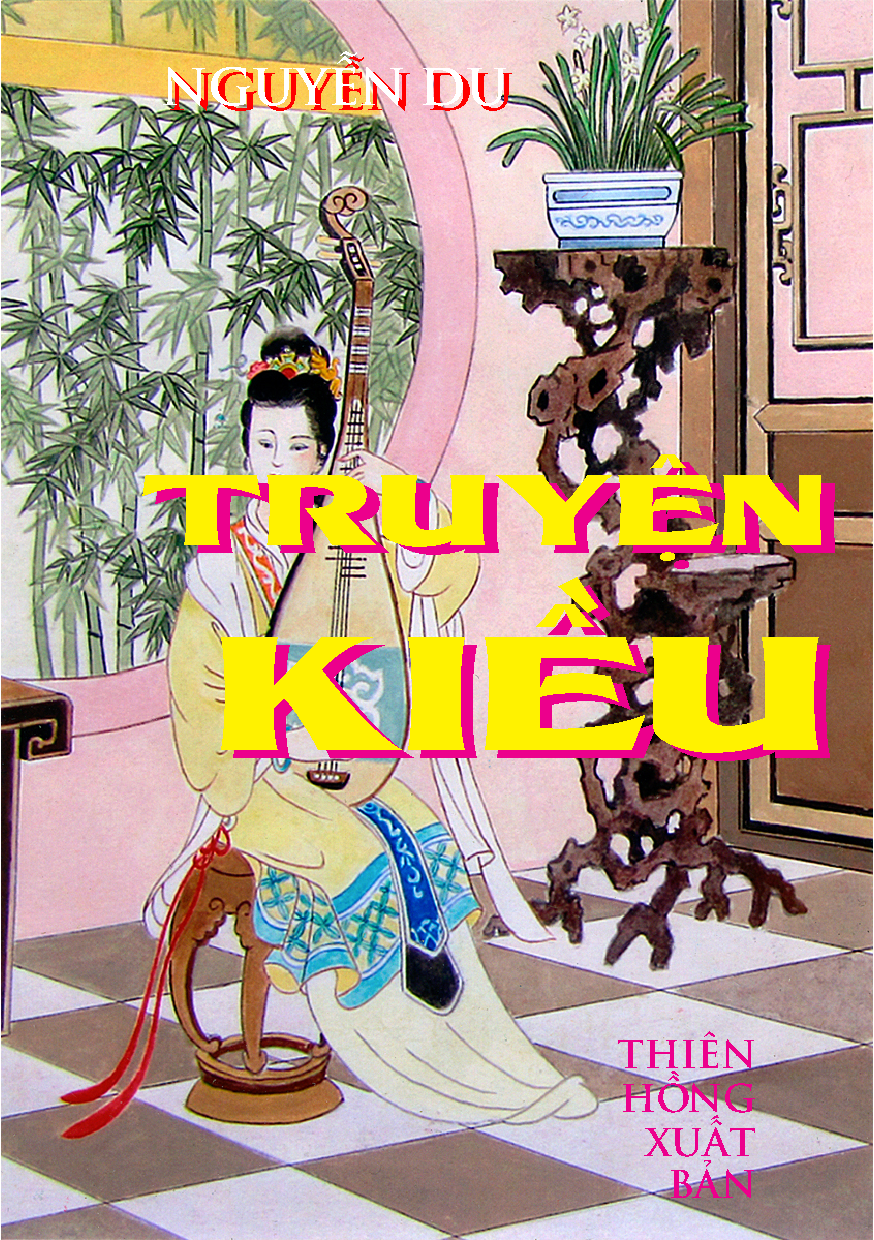
\includepdf[pages=-]{biasongkieu16feb20.pdf}

\newpage\ \vspace*{15.5cm}
\thispagestyle{empty}
\hrule 
\begin{flushright}
{\setmainfont{Times New Roman} Bìa 1: Tranh minh họa truyện Kiều của họa sĩ Anh Quân }
\end{flushright}


\newpage \ \vfill 

{\nguquoc  Đây  là bản  đánh máy lại  {\quocngu Truyện Kiều} bản in năm 1902 do cụ Phó bảng Kiều Oánh Mậu thực hiện với trang bìa tên là: {\quocngu Đoạn Trường Tân Thanh}.

\begin{enumerate}
\item Font chữ Nôm và chữ quốc ngữ {\nguquoc (cùng một bộ font)} của quyển sách này là\ {\nguquoc Nom Na Tong} của Hội Bảo tồn và Phát triển Di sản chữ Nôm, các font chữ quốc ngữ còn lại là\ {\nguquoc Times New Roman}.
\item Tysetting by {\setmainfont{Times New Roman}\selectfont \LaTeX\ - Nguyễn Thái Sơn}
\end{enumerate}}

\begin{flushright}
{\nguquoc Thành phố Hồ Chí Minh \today}
\end{flushright}


\thispagestyle{empty} \newpage \thispagestyle{empty} 

\ThisCenterWallPaper{1}{bia1.jpg}

\vspace*{1.25cm}

{\quocngu \hspace*{.25cm} vọng \hspace*{1cm}  thu\hspace*{1cm} trung\hspace*{1cm} dần\hspace*{1cm} nhâm\hspace*{.8cm} Thái\hspace*{1cm} Thành }

(đọc ngược)\vspace*{.6cm}

\begin{center}
 {\quocngu Đoạn}
 \end{center} 
 
 \vspace*{2.5cm}

\begin{center}
 {\quocngu Trường}
 \end{center} 
 
  \vspace*{3.25cm}

\begin{center}
 {\quocngu Tân}
 \end{center} 
    \vspace*{2.75cm}

\begin{center}
 {\quocngu Thanh}
 \end{center} 

\newpage \thispagestyle{empty}

\def\Ả{妸\kern.125em } 
\def\ả{婀\kern.125em } 

\def\ác{惡\kern.125em } 
\def\Ác{鵶\kern.125em } 

\def\ai{埃\kern.125em } 
\def\ái{愛\kern.125em } 
\def\ầm{喑\kern.125em } 
\def\am{庵\kern.125em } 
\def\ấm{廕\kern.125em } 
\def\ám{暗\kern.125em } 
\def\Ấm{蔭\kern.125em } 

\def\âm{陰\kern.125em } 
\def\Âm{音\kern.125em } 

\def\ấn{印\kern.125em } 
\def\ăn{咹\kern.125em } 

\def\an{鞍\kern.125em } 
\def\An{安\kern.125em } 

\def\ân{恩\kern.125em } 
\def\án{案\kern.125em } 
\def\Ân{殷\kern.125em } 
\def\ẩn{隱\kern.125em } 
\def\áng{盎\kern.125em } 

\def\anh{纓\kern.125em } 
\def\ANH{英\kern.125em } 
\def\Anh{鸚\kern.125em } 
\def\ANh{鸚\kern.125em } 

\def\ào{𠯻\kern.125em } 
\def\ao{呦\kern.125em } 
\def\áo{襖\kern.125em } 
\def\áp{押\kern.125em } 

\def\ấp{挹\kern.125em } 
\def\Ấp{邑\kern.125em } 

\def\ắt{乙\kern.125em } 
\def\âu{歐\kern.125em } 
\def\ấy{意\kern.125em } 
\def\áy{曖\kern.125em } 
\def\ba{𠀧\kern.125em } 
\def\bá{伯\kern.125em } 
\def\bã{把\kern.125em } 
\def\bả{把\kern.125em } 
\def\Ba{波\kern.125em } 

\def\bà{𱙘\kern.125em }   %\def\bà{\char 202328\kern.125em }
\def\Bà{婆\kern.125em } 

\def\bắc{北\kern.125em } 
\def\bác{博\kern.125em } 
\def\bậc{堛\kern.125em } 
\def\BẠc{泊\kern.125em } 
\def\bấc{苝\kern.125em } 
\def\bạc{萡\kern.125em } 
\def\Bạc{薄\kern.125em } 
\def\BẠC{鉑\kern.125em } 
\def\bách{柏\kern.125em } 
\def\bạch{白\kern.125em } 
\def\Bai{𠾦\kern.125em } 
\def\BÀi{婆\kern.125em } 
\def\bái{拜\kern.125em } 

\def\bài{排\kern.125em } 
\def\Bài{牌\kern.125em } 

\def\bai{𢴾\kern.125em } 
\def\bạn{伴\kern.125em } 
\def\bán{半\kern.125em } 
\def\bắn{𢏑\kern.125em } 
\def\bằn{弼\kern.125em } 

\def\bản{本\kern.125em } 
\def\Bản{板\kern.125em } 

\def\ban{班\kern.125em } 
\def\Ban{頒\kern.125em } 

\def\bàn{盘\kern.125em } 
\def\Bàn{盤\kern.125em } 

\def\bận{絆\kern.125em } 

\def\BĂng{冰\kern.125em } 
\def\Bằng{平\kern.125em } 

\def\bàng{徬\kern.125em } 
\def\Bàng{㥬\kern.125em } 

\def\bằng{朋\kern.125em } 
\def\bảng{榜\kern.125em } 

\def\băng{氷\kern.125em } 
\def\Băng{𨀰\kern.125em } 

\def\bâng{氷\kern.125em } 

\def\BẰng{鵬\kern.125em } 
\def\bành{彭\kern.125em } 
\def\bảnh{秉\kern.125em } 
\def\bánh{𨋣\kern.125em } 
\def\bao{包\kern.125em } 
\def\báo{報\kern.125em } 

\def\bào{胞\kern.125em } 
\def\Bào{袍\kern.125em } 
\def\BÀo{鉋\kern.125em } 


\def\bảo{保\kern.125em } 
\def\BẢo{宝\kern.125em } 
\def\Bảo{𠶓\kern.125em } 


\def\bất{不\kern.125em } 
\def\bát{八\kern.125em } 
\def\bặt{弼\kern.125em } 
\def\bắt{扒\kern.125em } 
\def\báu{宝\kern.125em } 
\def\bầu{瓢\kern.125em } 
\def\bâu{袍\kern.125em } 
\def\bầy{𠍣\kern.125em } 

\def\bay{𢒎\kern.125em } 
\def\Bay{𠎩\kern.125em } 

\def\Bây{𠾦\kern.125em } 
\def\bây{悲\kern.125em } 
\def\BÂy{碑\kern.125em } 


\def\Bấy{悲\kern.125em } 
\def\bày{排\kern.125em } 


\def\bấy{闭\kern.125em } 
\def\bảy{𬙞\kern.125em } 
\def\bẽ{𢜢\kern.125em } 
\def\bẻ{𢯏\kern.125em } 
\def\bể{𣷭\kern.125em } 
\def\bè{𤿤\kern.125em } 
\def\bến{𣷷\kern.125em } 
\def\bén{𤊰\kern.125em } 
\def\bên{边\kern.125em } 
\def\bèo{䕯\kern.125em } 

\def\bề{皮\kern.125em } 
\def\Bề{鼙\kern.125em } 

\def\bỉ{彼\kern.125em } 
\def\bi{悲\kern.125em } 
\def\bì{皮\kern.125em } 
\def\bia{碑\kern.125em } 
\def\bích{碧\kern.125em } 
\def\biếc{碧\kern.125em } 

\def\biến{变\kern.125em } 
\def\Biến{變\kern.125em }  

\def\biện{辨\kern.125em } 
\def\biên{边\kern.125em } 

\def\biếng{怲\kern.125em } 
\def\biết{別\kern.125em } 
\def\biệt{別\kern.125em } 
\def\bìm{𦹴\kern.125em } 
\def\binh{兵\kern.125em } 

\def\BÌNh{屏\kern.125em } 
\def\BÌnh{平\kern.125em } 
\def\bình{瓶\kern.125em } 
\def\Bình{𤭸\kern.125em } 
\def\BÌNH{萍\kern.125em } 


\def\bít{捌\kern.125em } 
\def\Bó{咘\kern.125em } 
\def\BÓ{咘\kern.125em } 
\def\bõ{哺\kern.125em } 
\def\Bõ{𡀨\kern.125em } 
\def\bờ{坡\kern.125em } 
\def\bơ{巴\kern.125em } 
\def\bố{布\kern.125em } 
\def\bó{抪\kern.125em } 
\def\bộ{步\kern.125em } 
\def\Bồ{菩\kern.125em } 
\def\bồ{蒲\kern.125em } 
\def\bỏ{補\kern.125em } 
\def\bò{𨆶\kern.125em } 
\def\Bộ{部\kern.125em } 
\def\bốc{卜\kern.125em } 
\def\bộc{濮\kern.125em } 
\def\bọc{纀\kern.125em } 
\def\bọc{纀\kern.125em } 
\def\bội{佩\kern.125em } 
\def\Bội{佩\kern.125em } 
\def\bội{倍\kern.125em } 
\def\bồi{培\kern.125em } 
\def\BỒi{徘\kern.125em } 
\def\bời{排\kern.125em } 
\def\bởi{𤳄\kern.125em } 
\def\Bởi{𪽝\kern.125em } 
\def\bối{貝\kern.125em } 
\def\bói{𧴤\kern.125em } 
\def\bói{𧴤\kern.125em } 
\def\Bồi{賠\kern.125em } 
\def\bợm{姂\kern.125em } 
\def\bốn{𦊚\kern.125em } 
\def\bỗng{俸\kern.125em } 
\def\bổng{俸\kern.125em } 
\def\bòng{𢸚\kern.125em } 
\def\Bồng{𢸚\kern.125em } 
\def\Bòng{𣠑\kern.125em } 
\def\bông{芃\kern.125em } 
\def\bồng{蓬\kern.125em } 
\def\bóng{𩃳\kern.125em } 
\def\bột{孛\kern.125em } 
%\def\bột{孛\kern.125em } 
\def\bớt{扒\kern.125em } 
\def\bọt{浡\kern.125em } 
\def\Bọt{渤\kern.125em } 
\def\bù{蒲\kern.125em } 
\def\búa{斧\kern.125em } 
\def\Búa{鈽\kern.125em } 
\def\bữa{𩛷\kern.125em } 
\def\bực{堛\kern.125em } 
\def\bức{幅\kern.125em } 
\def\BỤi{𡏧\kern.125em } 
\def\bụi{𣻃\kern.125em } 
\def\Bụi{蓓\kern.125em } 
\def\bùi{𫬍\kern.125em } 
\def\bùn{𡎛\kern.125em } 
\def\bưng{𢬄\kern.125em } 
\def\bừng{𤇊\kern.125em } 
\def\bụng{䏾\kern.125em } 
\def\Buộc{𢯜\kern.125em } 
\def\buộc{𫃚񣡎\kern.125em } 
\def\BUỘc{𥾾\kern.125em } 
\def\BUộc{𦄾\kern.125em } 
\def\bước{𨀈\kern.125em } 
\def\buổi{𣇜\kern.125em } 
\def\buồm{帆\kern.125em } 
\def\bướm{𧊉\kern.125em } 
\def\buôn{奔\kern.125em } 
\def\buồn{𢞂\kern.125em } 
\def\Buông{𡍙\kern.125em } 
\def\buồng{𢩣\kern.125em } 
\def\buông{𢭾\kern.125em } 
\def\bút{筆\kern.125em } 
\def\cả{奇\kern.125em } 
\def\Ca{𰙔\kern.125em } 
\def\ca{歌\kern.125em } 
\def\cà{袈\kern.125em } 
\def\cá{𩵜\kern.125em } 
\def\Các{各\kern.125em } 
\def\các{閣\kern.125em } 
\def\CÁch{格\kern.125em } 
\def\cách{隔\kern.125em } 
\def\Cách{革\kern.125em } 
\def\cái{丐\kern.125em } 
\def\Cái{蓋\kern.125em } 
\def\cài{掑\kern.125em } 
\def\cãi{改\kern.125em } 
\def\Cải{改\kern.125em } 
\def\cải{𦰦\kern.125em } 
\def\căm{㤌\kern.125em } 
\def\cám{感\kern.125em } 
\def\cảm{感\kern.125em } 
\def\cầm{扲\kern.125em } 
\def\Cầm{琴\kern.125em } 
\def\CẦm{岌\kern.125em } 
\def\cam{甘\kern.125em } 
\def\cẩm{錦\kern.125em } 
\def\càn{乾\kern.125em } 
\def\cần{勤\kern.125em } 
\def\cắn{哏\kern.125em } 
\def\Cạn{𠲟\kern.125em } 
\def\Cân{巾\kern.125em } 
\def\can{干\kern.125em } 
\def\cân{斤\kern.125em } 
\def\căn{根\kern.125em } 
\def\cạn{𣴓\kern.125em } 
\def\Can{肝\kern.125em } 
\def\Cần{芹\kern.125em } 
\def\càng{強\kern.125em } 
\def\cảnh{景\kern.125em } 
\def\canh{更\kern.125em } 
\def\Cánh{更\kern.125em } 
\def\cành{梗\kern.125em } 
\def\cánh{𦑃\kern.125em } 
\def\cáo{告\kern.125em } 
\def\cao{皋\kern.125em } 
\def\cảo{稿\kern.125em } 
\def\Cao{高\kern.125em } 
\def\cắp{𠎨\kern.125em } 
\def\Cập{及\kern.125em } 
\def\cập{岌\kern.125em } 
\def\cặp{𥝥\kern.125em } 
\def\cắt{割\kern.125em } 
\def\cất{拮\kern.125em } 
\def\cát{洁\kern.125em } 
\def\Cát{㵧\kern.125em } 
\def\CÁt{葛\kern.125em } 
\def\câu{勾\kern.125em } 
\def\cấu{垢\kern.125em } 
\def\cầu{捄\kern.125em } 
\def\Cầu{求\kern.125em } 
\def\CẦu{橋\kern.125em } 
\def\CẦU{毬\kern.125em } 
\def\cẦu{梂\kern.125em } 
\def\cậu{舅\kern.125em } 
\def\Cấu{逅\kern.125em } 
\def\Câu{駒\kern.125em } 
\def\cay{𠹽\kern.125em } 
\def\cậy{𢚁\kern.125em } 
\def\cây{𣘃\kern.125em } 
\def\chạ{乍\kern.125em } 
\def\cha{吒\kern.125em } 
\def\chã{𣾻\kern.125em } 
\def\chác{卓\kern.125em } 
\def\Chắc{𠺵\kern.125em } 
\def\CHắc{聀\kern.125em } 
\def\chắc{質\kern.125em } 
\def\chái{厔\kern.125em } 
\def\chải{扯\kern.125em } 
\def\chài{𦄴\kern.125em } 
\def\chăm{𢟙\kern.125em } 
\def\Chạm{𪮻\kern.125em } 
\def\chạm{湛\kern.125em } 
\def\chàm{藍\kern.125em } 
\def\chấm{譖\kern.125em } 
\def\chan{滇\kern.125em } 
\def\chăn{𧜖\kern.125em } 
\def\chân{蹎\kern.125em } 
\def\chán{󰇏\kern.125em } 
\def\Chán{󱋓\kern.125em } 
\def\chăng{庄\kern.125em } 
\def\Chẳng{庄\kern.125em } 
\def\chàng{払\kern.125em } 
\def\chẳng{拯\kern.125em } 
\def\chạnh{𢤜\kern.125em } 
\def\CHạnh{擲\kern.125em } 
\def\chanh{爭\kern.125em } 
\def\Chạnh{鄭\kern.125em } 
\def\chào{嘲\kern.125em } 
\def\chấp{執\kern.125em } 
\def\chập{執\kern.125em } 
\def\chắp{执\kern.125em } 
\def\Chắp{插\kern.125em } 
\def\chặt{秩\kern.125em } 
\def\chật{秩\kern.125em } 
\def\chất{質\kern.125em } 
\def\Chặt{質\kern.125em } 
\def\chầu{𠎫\kern.125em } 
\def\chau{咮\kern.125em } 
\def\CHau{𠺾\kern.125em } 
\def\chậu{𡊱\kern.125em } 
\def\cháu{𡥙\kern.125em } 
\def\Châu{州\kern.125em } 
\def\CHâu{朱\kern.125em } 
\def\châu{珠\kern.125em } 
\def\Chau{𤶎\kern.125em } 
\def\chày{𣖖\kern.125em } 
\def\chảy{沚\kern.125em } 
\def\cháy{𤈜\kern.125em } 
\def\Chạy{𧼋\kern.125em } 
\def\chạy{𬦳\kern.125em } 
\def\chầy{迡\kern.125em } 
\def\chay{齋\kern.125em } 
\def\chế{制\kern.125em } 
\def\chê{吱\kern.125em } 
\def\Chề{𠽮\kern.125em } 
\def\chẻ{扯\kern.125em } 
\def\chè{茶\kern.125em } 
\def\chề{迡\kern.125em } 
\def\che{𩂏\kern.125em } 
\def\chếch{隻\kern.125em } 
\def\chém{㓠\kern.125em } 
\def\chén{𡃹\kern.125em } 
\def\Chen{扦\kern.125em } 
\def\chen{𢫔\kern.125em } 
\def\CHEn{擅\kern.125em } 
\def\CHen{𦍫\kern.125em } 
\def\CHEN{羶\kern.125em } 
\def\chênh{征\kern.125em } 
\def\Chênh{隻\kern.125em } 
\def\chèo{棹\kern.125em } 
\def\chéo{𧝨\kern.125em } 
\def\chép{劄\kern.125em } 
\def\chết{𣨰\kern.125em } 
\def\chi{之\kern.125em } 
\def\chỉ{只\kern.125em } 
\def\chị{姉\kern.125em } 
\def\chí{志\kern.125em } 
\def\CHỉ{指\kern.125em } 
\def\Chỉ{旨\kern.125em } 
\def\CHỈ{𥿗\kern.125em } 
\def\chì{鈘\kern.125em } 
\def\Chia{𢺹\kern.125em } 
\def\chia{𢺺\kern.125em } 
\def\CHIA{𢺺\kern.125em } 
\def\CHia{󰯞\kern.125em } 
\def\chiếc{隻\kern.125em } 
\def\chiêm{占\kern.125em } 
\def\chiếm{占\kern.125em } 
\def\chiến{戰\kern.125em } 
\def\chiềng{𠴔\kern.125em } 
\def\chiếng{𦭒\kern.125em } 
\def\chiêng{鉦\kern.125em } 
\def\Chiêng{鼙\kern.125em } 
\def\chiết{淅\kern.125em } 
\def\Chiêu{招\kern.125em } 
\def\chiêu{昭\kern.125em } 
\def\chiều{朝\kern.125em } 
\def\chiếu{照\kern.125em } 
\def\Chiếu{詔\kern.125em } 
\def\chìm{沉\kern.125em } 
\def\chim{𪀄\kern.125em } 
\def\chín{𠃩\kern.125em } 
\def\chỉn{㐱\kern.125em } 
\def\Chỉn{診\kern.125em } 
\def\chinh{征\kern.125em } 
\def\chỉnh{整\kern.125em } 
\def\chính{正\kern.125em } 
\def\chịu{𠹾\kern.125em } 
\def\chớ{𠤆\kern.125em } 
\def\chợ{𢄂\kern.125em } 
\def\cho{朱\kern.125em } 
\def\chơ{猪\kern.125em } 
\def\chờ{除\kern.125em } 
\def\chở{𩅻\kern.125em } 
\def\choáng{𤶏\kern.125em } 
\def\chọc{𢹅\kern.125em } 
\def\chốc{祝\kern.125em } 
\def\chồi{𣑳\kern.125em } 
\def\chơi{𨔈\kern.125em } 
\def\chốn{准\kern.125em } 
\def\chôn{墫\kern.125em } 
\def\chờn{廛\kern.125em } 
\def\chọn{𢮪\kern.125em } 
\def\Chọn{撰\kern.125em } 
\def\chồn{𤶐\kern.125em } 
\def\Chồng{𥔧\kern.125em } 
\def\CHỒNG{\char 989145\kern.125em } %󰣆\ }
\def\chồng{𫯳\kern.125em } 
\def\chong{炵\kern.125em } 
\def\Chong{𤍑\kern.125em } 
\def\chông{蔠\kern.125em } 
\def\chót{啐\kern.125em } 
\def\chợt{秩\kern.125em } 
\def\chủ{主\kern.125em } 
\def\chu{周\kern.125em } 
\def\Chữ{𡨸\kern.125em } 
\def\chữ{𫳘\kern.125em } 
\def\chú{註\kern.125em } 
\def\chư{諸\kern.125em } 
\def\chúa{主\kern.125em } 
\def\Chua{咮\kern.125em } 
\def\chùa{廚\kern.125em } 
\def\chưa{渚\kern.125em } 
\def\chửa{渚\kern.125em } 
\def\Chưa{猪\kern.125em } 
\def\chứa{躇\kern.125em } 
\def\chua{䣷\kern.125em } 
\def\chừa{除\kern.125em } 
\def\chực{直\kern.125em } 
\def\chục{𨔿\kern.125em } 
\def\chụm{笘\kern.125em } 
\def\chừng{澄\kern.125em } 
\def\chung{終\kern.125em } 
\def\chứng{証\kern.125em } 
\def\chùng{重\kern.125em } 
\def\Chung{鍾\kern.125em } 
\def\chước{斫\kern.125em } 
\def\Chuốc{祝\kern.125em } 
\def\chuộc{贖\kern.125em } 
\def\chuốc{酌\kern.125em } 
\def\chườn{𠴔\kern.125em } 
\def\chuồn{𧋃\kern.125em } 
\def\Chường{呈\kern.125em } 
\def\chường{悜\kern.125em } 
\def\chuông{鍾\kern.125em } 
\def\chương{章\kern.125em } 
\def\chuốt{捽\kern.125em } 
\def\Chuốt{淬\kern.125em } 
\def\Chút{少\kern.125em } 
\def\chút{𡭧\kern.125em } 
\def\chuyện{傳\kern.125em } 
\def\chuyên{專\kern.125em } 
\def\chuyển{轉\kern.125em } 
\def\Có{世\kern.125em } 
\def\có{固\kern.125em } 
\def\cơ{奇\kern.125em } 
\def\Cơ{機\kern.125em } 
\def\cƠ{基\kern.125em } 
\def\CƠ{机\kern.125em } 
\def\cô{姑\kern.125em } 
\def\Co{孤\kern.125em } 
\def\Cô{孤\kern.125em } 
\def\co{𢮩\kern.125em } 
\def\cớ{據\kern.125em } 
\def\cố{故\kern.125em } 
\def\cờ{旗\kern.125em } 
\def\Cờ{棊\kern.125em } 
\def\cỜ{棋\kern.125em } 
\def\CỜ{期\kern.125em }
\def \cờ棋{棋\kern.125em }
\def\cỏ{𦹵\kern.125em } 
\def\Cố{顧\kern.125em } 
\def\cò{𪂲\kern.125em } 
\def\cổ{古\kern.125em } 
\def\Cổ{鼓\kern.125em } 
\def\cố故{故\kern.125em } 
\def\cõi{𡎝\kern.125em } 
\def\cổi{𢶒\kern.125em } 
\def\Cởi{𢶒\kern.125em } 
\def\cởi{𢶷\kern.125em } 
\def\cội{檜\kern.125em } 
\def\coi{𥋳\kern.125em } 
\def\Cỗi{檜\kern.125em } 
\def\cỗi{𦓊\kern.125em } 
\def\còi{𧥇\kern.125em } 
\def\cơm{𩚵\kern.125em } 
\def\cồn{𡑱\kern.125em } 
\def\con{𡥵\kern.125em } 
\def\cơn{干\kern.125em } 
\def\Con{昆\kern.125em } 
\def\côn{棍\kern.125em } 
\def\còn{羣\kern.125em } 
\def\Còn{群\kern.125em } 
\def\cong{𢏢\kern.125em } 
\def\công{公\kern.125em } 
\def\Công{功\kern.125em } 
\def\CÔng{工\kern.125em } 
\def\CÔNg{攻\kern.125em } 
\def\cổng{槓\kern.125em } 
\def\cốt{傦\kern.125em } 
\def\cợt{𠹳\kern.125em } 
\def\Cốt{骨\kern.125em } 
\def\cù{劬\kern.125em } 
\def\cũ{𡳵\kern.125em } 
\def\cứ{據\kern.125em } 
\def\cữ{昛\kern.125em } 
\def\Cù{樛\kern.125em } 
\def\của{𧵑\kern.125em } 
\def\cưa{鋸\kern.125em } 

\def\Cửa{𬮌\kern.125em } 
\def\cửa{󰘂\kern.125em } 
\def\cửa{\char"F0567\kern.125em } 


\def\cực{極\kern.125em } 
\def\cúc{菊\kern.125em } 
\def\cúi{儈\kern.125em } 
\def\cũi{櫃\kern.125em } 
\def\Cúi{𩠴\kern.125em } 
\def\Cung{供\kern.125em } 
\def\cúng{供\kern.125em } 
\def\Cũng{共\kern.125em } 
\def\cứng{𠠊\kern.125em } 
\def\cung{宮\kern.125em } 
\def\CUng{工\kern.125em } 
\def\Cùng{共\kern.125em } 
\def\CÙng{拱\kern.125em } 
\def\CÙNG{穷\kern.125em } 
\def\cùng{窮\kern.125em } 
\def\cũng{拱\kern.125em } 
\def\cuộc{局\kern.125em } 
\def\cước{腳\kern.125em } 
\def\cười{唭\kern.125em } 
\def\cuối{𡳜\kern.125em } 
\def\cưỡi{騎\kern.125em } 
\def\cuốn{捲\kern.125em } 
\def\Cuốn{綣\kern.125em } 
\def\cường{強\kern.125em } 
\def\cương{綱\kern.125em } 
\def\cướp{刧\kern.125em } 
\def\cửu{九\kern.125em } 
\def\cứu{救\kern.125em } 
\def\cưu{鳩\kern.125em } 
\def\dã{也\kern.125em } 
\def\đã{㐌\kern.125em } 
\def\đà{它\kern.125em } 
\def\Đà{佗\kern.125em } 
\def\đÀ{拖\kern.125em } 
\def\ĐÀ{陀\kern.125em } 
\def\dạ{𠰺\kern.125em } 
\def\Dạ{胣\kern.125em } 
\def\DẠ{夜\kern.125em } 
\def\dẠ{㖡\kern.125em } 
\def\đa{多\kern.125em } 
\def\đá{𥒥\kern.125em } 
\def\Đá{𥒥\kern.125em } 
\def\da{䏧\kern.125em } 
\def\dà{茄\kern.125em } 
\def\ĐÁ{跢\kern.125em } 
\def\dặc{弋\kern.125em } 
\def\đắc{得\kern.125em } 
\def\đặc{特\kern.125em } 
\def\đãi{代\kern.125em } 
\def\Đại{代\kern.125em } 
\def\dai{佳\kern.125em } 
\def\đại{大\kern.125em } 
\def\Đài{它\kern.125em } 
\def\đai{帶\kern.125em } 
\def\đãi{待\kern.125em } 
\def\dãi{𤋵\kern.125em } 
\def\dại{𤵺\kern.125em } 
\def\DẢI{繲\kern.125em } 
\def\đài{臺\kern.125em } 
\def\DẢi{𧞊\kern.125em } 
\def\dải{解\kern.125em } 
\def\Dải{觧\kern.125em } 
\def\dài{𨱽\kern.125em } 
\def\dạm{啖\kern.125em } 
\def\Dạm{𡃞\kern.125em } 
\def\đâm{抌\kern.125em } 
\def\đạm{淡\kern.125em } 
\def\dâm{淫\kern.125em } 
\def\dầm{淫\kern.125em } 
\def\đăm{㴷\kern.125em } 
\def\đắm{㴷\kern.125em } 
\def\đằm{潭\kern.125em } 
\def\đầm{潭\kern.125em } 
\def\dám{监\kern.125em } 
\def\Dám{監\kern.125em } 
\def\dàm{緘\kern.125em } 
\def\dấm{𨡉\kern.125em } 
\def\dặm{𨤮\kern.125em } 
\def\Dặm{𨤵\kern.125em } 
\def\dặn{吲\kern.125em } 
\def\đan{單\kern.125em } 
\def\đắn{坦\kern.125em } 
\def\Đàn{𡊨\kern.125em } 
\def\ĐÀn{壇\kern.125em } 
\def\đàn{弹\kern.125em } 
\def\ĐÀN{彈\kern.125em } 
\def\dần{寅\kern.125em } 
\def\dẫn{引\kern.125em } 
\def\dạn{惮\kern.125em } 
\def\đặn{惮\kern.125em } 
\def\dan{𢬥\kern.125em } 
\def\Dần{𢴍\kern.125em } 
\def\Dan{攔\kern.125em } 
\def\dàn{攔\kern.125em } 
\def\dân{民\kern.125em } 
\def\dấn{𤄱\kern.125em } 
\def\đấng{𠎬\kern.125em } 
\def\dặng{𠱆\kern.125em } 
\def\Dàng{𠲞\kern.125em } 
\def\Đắng{𡃻\kern.125em } 
\def\Đàng{堂\kern.125em } 
\def\đàng{塘\kern.125em } 
\def\dắng{孕\kern.125em } 
\def\Dằng{弋\kern.125em } 
\def\ĐẮng{𢚸\kern.125em } 
\def\dàng{𢬥\kern.125em } 
\def\dang{揚\kern.125em } 
\def\dáng{樣\kern.125em } 
\def\dạng{樣\kern.125em } 
\def\dằng{浪\kern.125em } 
\def\đang{當\kern.125em } 
\def\đáng{當\kern.125em } 
\def\dâng{𤼸\kern.125em } 
\def\đẳng{等\kern.125em } 
\def\đãng{蕩\kern.125em } 
\def\đắng{䔲\kern.125em }  
\def\ĐẰng{藤\kern.125em } 
\def\dắng{賸\kern.125em } 
\def\đằng{鄧\kern.125em } 
\def\đẵng{鄧\kern.125em } 
\def\Đằng{騰\kern.125em } 
\def\đành{仃\kern.125em } 
\def\dành{伶\kern.125em } 
\def\danh{名\kern.125em } 
\def\Dành{𠯼\kern.125em } 
\def\DÀnh{𠴔\kern.125em } 
\def\Đành{忊\kern.125em } 
\def\đánh{打\kern.125em } 
\def\đảo{倒\kern.125em } 
\def\dao{刀\kern.125em } 
\def\đao{刀\kern.125em } 
\def\Đảo{島\kern.125em } 
\def\đào{桃\kern.125em } 
\def\Đào{濤\kern.125em } 
\def\dào{𤁓\kern.125em } 
\def\Dao{瑤\kern.125em } 
\def\dạo{𨄹\kern.125em } 
\def\đạo{道\kern.125em } 
\def\DAo{遙\kern.125em } 
\def\đắp{塔\kern.125em } 
\def\dập{拉\kern.125em } 
\def\đập{拉\kern.125em } 
\def\đáp{答\kern.125em } 
\def\Dập{習\kern.125em } 
\def\đạp{踏\kern.125em } 
\def\đặt{噠\kern.125em } 
\def\đắt{𠿲\kern.125em } 
\def\đất{坦\kern.125em } 
\def\dắt{𢴑\kern.125em } 
\def\DẮt{㩫\kern.125em } 
\def\Dắt{𦄵\kern.125em } 
\def\Dặt{迭\kern.125em } 
\def\dặt{逸\kern.125em } 
\def\Đặt{達\kern.125em } 
\def\Dâu{兜\kern.125em } 
\def\đâu{兜\kern.125em } 
\def\Dầu{𠱋\kern.125em } 
\def\Dấu{唒\kern.125em } 
\def\Dẫu{唒\kern.125em } 
\def\DÂu{妯\kern.125em } 
\def\đầu{投\kern.125em } 
\def\đậu{杜\kern.125em } 
\def\dâu{橷\kern.125em } 
\def\dàu{油\kern.125em } 
\def\dầu{油\kern.125em } 
\def\đau{𤴬\kern.125em } 
\def\dấu{𨁪\kern.125em } 
\def\dẫu{酉\kern.125em } 
\def\Đầu{頭\kern.125em } 
\def\đây{低\kern.125em } 
\def\dày{𠫅\kern.125em } 
\def\dầy{𠫅\kern.125em } 
\def\Dày{𠫆\kern.125em } 
\def\Dầy{𠫆\kern.125em } 
\def\dạy{𠰺\kern.125em } 
\def\dãy{圯\kern.125em } 
\def\đấy{帝\kern.125em } 
\def\đáy{底\kern.125em } 
\def\đẫy{悌\kern.125em } 
\def\đẩy{𢩽\kern.125em } 
\def\dẫy{汜\kern.125em } 
\def\Đày{𣹓\kern.125em } 
\def\đầy{𣹓\kern.125em } 
\def\dây{𦀊\kern.125em } 
\def\DÀy{苔\kern.125em } 
\def\đày{苔\kern.125em } 
\def\ĐẦy{苔\kern.125em } 
\def\Đầy{𧀟\kern.125em } 
\def\dấy{𧻭\kern.125em } 
\def\dậy{𠰺\kern.125em } 
\def\Dậy{𧻭\kern.125em } 
\def\Dè{𠽮\kern.125em } 
\def\đế{帝\kern.125em } 
\def\để{底\kern.125em } 
\def\Để{抵\kern.125em } 
\def\dè{提\kern.125em } 
\def\đè{提\kern.125em } 
\def\đề{提\kern.125em } 
\def\dễ{易\kern.125em } 
\def\Dề{𣾸\kern.125em } 
\def\dề{題\kern.125em } 
\def\đà拖{拖\kern.125em } 
\def\Đề{題\kern.125em } 
\def\đêm{𣈘\kern.125em } 
\def\Đêm{𣎀\kern.125em } 
\def\đem{󰝂\kern.125em } 


\def\Đến{典\kern.125em } 
\def\đền{𡊰\kern.125em } 
\def\đến{旦\kern.125em } 
\def\đèn{畑\kern.125em } 
\def\đen{顛\kern.125em } 
\def\đênh{汀\kern.125em } 
\def\đeo{㧅\kern.125em } 
\def\đèo{㧅\kern.125em } 
\def\ĐẸP{惵\kern.125em } 
\def\dẹp{揲\kern.125em } 
\def\đẹp{𬙾\kern.125em } 
\def\đẹp{𬙾\kern.125em } 
\def\dệt{𦄅\kern.125em } 
\def\đều{調\kern.125em } 
\def\đi{𠫾\kern.125em } 
\def\dĩ{𡵆\kern.125em } 
\def\Di{移\kern.125em } 
\def\di{遺\kern.125em } 
\def\địa{地\kern.125em } 
\def\đìa{𣾸\kern.125em } 
\def\đĩa{𥒃\kern.125em } 
\def\dịch{役\kern.125em } 
\def\đích{的\kern.125em } 
\def\điếc{𦖡\kern.125em } 
\def\điếm{店\kern.125em } 
\def\điểm{點\kern.125em } 
\def\diễn{演\kern.125em } 
\def\điền{田\kern.125em } 
\def\diện{面\kern.125em } 
\def\diệp{葉\kern.125em } 
\def\điệp{蝶\kern.125em } 
\def\diệu{妙\kern.125em } 
\def\ĐIều{桃\kern.125em } 
\def\Điều{條\kern.125em } 
\def\Điệu{窕\kern.125em } 
\def\điều{調\kern.125em } 
\def\điệu{調\kern.125em } 
\def\điêu{貂\kern.125em } 
\def\đinh{丁\kern.125em } 
\def\Đinh{釘\kern.125em } 
\def\đình{亭\kern.125em } 
\def\định{定\kern.125em } 
\def\Đình{庭\kern.125em } 
\def\ĐÌnh{廷\kern.125em } 
\def\ĐÌNh{霆\kern.125em } 
\def\đỉnh{頂\kern.125em } 
\def\Đỉnh{鼎\kern.125em } 
\def\dịp{堞\kern.125em } 
\def\Dìu{妙\kern.125em } 
\def\dịu{妙\kern.125em } 
\def\díu{𢬢\kern.125em } 
\def\dìu{迢\kern.125em } 
\def\DÌu{迢\kern.125em } 
\def\dỗ{𠴗\kern.125em } 
\def\dò{𠻀\kern.125em } 
\def\đồ{圖\kern.125em } 
\def\Đồ{塗\kern.125em } 
\def\đó{妬\kern.125em } 
\def\đố{妬\kern.125em } 
\def\độ{度\kern.125em } 
\def\đỡ{拖\kern.125em } 
\def\đo{𢵋\kern.125em } 
\def\dở{𢷣\kern.125em } 
\def\đỗ{杜\kern.125em } 
\def\dơ{𬉣\kern.125em } 
\def\đổ{睹\kern.125em }  
\def\đò{艔\kern.125em } 
\def\Đổ{覩\kern.125em } 
\def\đỏ{𧺃\kern.125em } 
\def\đô{都\kern.125em } 
\def\Dở{󰇾\kern.125em } 
\def\đoạ{墮\kern.125em } 
\def\Đóa{朵\kern.125em } 
\def\đoá{朶\kern.125em } 
\def\đóa{朶\kern.125em } 
\def\đoái{兑\kern.125em } 
\def\đoài{兑\kern.125em } 
\def\đoàn{團\kern.125em } 
\def\đoán{断\kern.125em } 
\def\Đoạn{断\kern.125em } 
\def\đoạn{斷\kern.125em } 
\def\ĐOạn{段\kern.125em } 
\def\đoan{端\kern.125em } 
\def\doanh{楹\kern.125em } 
\def\Doanh{营\kern.125em } 
\def\dọc{唷\kern.125em } 

%\def\Dọc{圤 \kern-.7em\raisebox{-.325ex}{\crule[white]{.4em}{2.2ex}}\kern-.7em 育} 
\def\Dọc{育\kern.125em }


\def\độc{毒\kern.125em } 
\def\đốc{督\kern.125em } 

\def\đời{𠁀\kern.125em } 
\def\đòi{𠾕\kern.125em } 
\def\dối{嚉\kern.125em } 
\def\doi{堆\kern.125em } 
\def\đôi{堆\kern.125em } 
\def\đỗi{𡑖\kern.125em } 
\def\đợi{待\kern.125em } 
\def\Dối{𢬭\kern.125em } 
\def\đổi{𢬭\kern.125em } 
\def\dồi{𣼭\kern.125em } 
\def\dời{移\kern.125em } 
\def\đội{隊\kern.125em } 
\def\đồi{頽\kern.125em } 
\def\dòm{𥉰\kern.125em } 
\def\đơn{丹\kern.125em } 
\def\Đơn{单\kern.125em } 
\def\đồn{吨\kern.125em } 
\def\Đón{噋\kern.125em } 
\def\Đồn{屯\kern.125em } 
\def\dồn{扽\kern.125em } 
\def\đòn{扽\kern.125em } 
\def\dọn{𢮪\kern.125em } 
\def\DỌn{撰\kern.125em } 
\def\Dọn{𢶿\kern.125em } 
\def\dòn{𣆱\kern.125em } 
\def\Đòn{杶\kern.125em } 
\def\don{𤈊\kern.125em } 
\def\đớn{疸\kern.125em } 
\def\đón{迍\kern.125em } 
\def\đồng{僮\kern.125em } 
\def\đong{冬\kern.125em } 
\def\Đông{冬\kern.125em } 
\def\động{動\kern.125em } 
\def\Đồng{同\kern.125em } 
\def\đóng{埬\kern.125em } 
\def\đống{埬\kern.125em } 
\def\Dong{容\kern.125em } 
\def\dông{容\kern.125em } 
\def\Đóng{㨂\kern.125em } 
\def\Đong{𣁲\kern.125em } 
\def\đông{東\kern.125em } 
\def\đông{東\kern.125em } 
\def\ĐỒNg{桐\kern.125em } 
\def\dòng{𣳔\kern.125em } 
\def\Động{洞\kern.125em } 
\def\dong{炵\kern.125em } 
\def\ĐỒNG{童\kern.125em } 
\def\đổng{董\kern.125em } 
\def\Đong{𨒟\kern.125em } 
\def\ĐỒng{銅\kern.125em } 
\def\dột{𢝀\kern.125em } 
\def\đốt{炪\kern.125em } 
\def\ĐỐt{焠\kern.125em } 
\def\Đốt{𦵛\kern.125em } 
\def\dữ{𭁈\kern.125em } 
\def\dù{油\kern.125em } 
\def\Du{游\kern.125em } 
\def\Đủ{睹\kern.125em } 
\def\du{遊\kern.125em } 
\def\dự{預\kern.125em } 
\def\dư{餘\kern.125em } 
\def\đủ{\char 205067\kern.125em }  
\def\đứa{𠀲\kern.125em } 
\def\đua{𢵋\kern.125em } 
\def\dưa{荼\kern.125em } 
\def\đưa{迻\kern.125em } 
\def\đức{德\kern.125em } 
\def\đục{濁\kern.125em } 
\def\Đúc{𤒘\kern.125em } 
\def\đúc{𨯹\kern.125em } 
\def\duềnh{溋\kern.125em } 
\def\dùi{椎\kern.125em } 
\def\đùm{𦅰\kern.125em } 
\def\Dừng{仃\kern.125em } 
\def\dưng{仍\kern.125em } 
\def\dũng{勇\kern.125em } 
\def\đùng{同\kern.125em } 
\def\dựng{孕\kern.125em } 
\def\Dung{容\kern.125em } 
\def\Dựng{𢫡\kern.125em } 
\def\DỪng{棱\kern.125em } 
\def\đừng{𣫲\kern.125em } 
\def\dùng{用\kern.125em } 
\def\dừng{𥩯\kern.125em } 
\def\đứng{𥪸\kern.125em } 
\def\dung{蓉\kern.125em } 
\def\DỪNg{𨀊\kern.125em } 
\def\Được{得\kern.125em } 
\def\đuốc{𤒘\kern.125em } 
\def\được{特\kern.125em } 
\def\đuôi{𡳪\kern.125em } 
\def\dưới{𤲂\kern.125em } 
\def\đuổi{𨆏\kern.125em } 
\def\Đuổi{𨆷\kern.125em } 
\def\Đượm{淡\kern.125em } 
\def\đượm{㷋\kern.125em }  
\def\ĐƯờng{唐\kern.125em } 
\def\Đường{堂\kern.125em } 
\def\đường{塘\kern.125em } 
\def\dương{楊\kern.125em } 
\def\đương{當\kern.125em } 
\def\Dương{陽\kern.125em } 
\def\dưỡng{養\kern.125em } 
\def\dường{󰟯\kern.125em } 
\def\Dường𠍵{𠍵\kern.125em } 
\def\DỨt{𠞹\kern.125em } 
\def\Đứt{𠞹\kern.125em } 
\def\Dứt{悉\kern.125em } 
\def\dứt{𢴑\kern.125em } 
\def\đứt{䋎\kern.125em } 
\def\duyên{緣\kern.125em } 
\def\e{𠲖\kern.125em } 
\def\Ê{𠲖\kern.125em } 
\def\E{𠵱\kern.125em } 
\def\ê{醯\kern.125em } 
\def\em{㛪\kern.125em } 
\def\êm{淹\kern.125em } 
\def\én{燕\kern.125em } 
\def\ÉP{𠶟\kern.125em } 
\def\ép{壓\kern.125em } 
\def\Ép{押\kern.125em } 
\def\gã{𡥚\kern.125em } 
\def\gà{𪃴\kern.125em } 
\def\Gà{𬷤\kern.125em } 
\def\GÁC{挌\kern.125em } 
\def\Gác{搁\kern.125em } 
\def\GÁc{閣\kern.125em } 
\def\gác{阁\kern.125em } 
\def\gÁc{𣴜\kern.125em } 
\def\gái{𡛔\kern.125em } 
\def\gai{荄\kern.125em } 
\def\gấm{錦\kern.125em } 
\def\gắn{哏\kern.125em } 
\def\gạn{𠲟\kern.125em } 
\def\GẠn{𠴞\kern.125em } 
\def\Gạn{𢭬\kern.125em } 
\def\gàn{㨴\kern.125em } 
\def\gán{擀\kern.125em } 
\def\gan{肝\kern.125em } 
\def\gần{𧵆\kern.125em } 
\def\gang{𡬼\kern.125em } 
\def\gàng{強\kern.125em } 
\def\gánh{挭\kern.125em } 
\def\gấp{𠍭\kern.125em } 
\def\gập{岌\kern.125em } 
\def\gặp{﨤\kern.125em } 
\def\gạt{拔\kern.125em } 
\def\gật{𩠓\kern.125em } 
\def\gáy{嘅\kern.125em } 
\def\gãy{技\kern.125em } 
\def\gảy{𢭮\kern.125em } 
\def\gày{𤷍\kern.125em } 
\def\gầy{𤷍\kern.125em } 
\def\gây{𨢟\kern.125em } 
\def\ghê{𠺳\kern.125em } 
\def\Ghê{𡃊\kern.125em } 
\def\Ghé{㨳\kern.125em } 
\def\ghế{槣\kern.125em } 
\def\ghẻ{𤴪\kern.125em } 
\def\ghé{𥊘\kern.125em } 
\def\ghen{慳\kern.125em } 
\def\ghềnh{𡌿\kern.125em } 
\def\GHềnh{𡹡\kern.125em } 
\def\Ghềnh{涼\kern.125em } 
\def\ghét{恄\kern.125em } 
\def\ghé㨳{㨳\kern.125em } 
\def\ghé𥊘{𥊘\kern.125em } 
\def\ghi{𥱬\kern.125em } 
\def\Gì{之\kern.125em } 
\def\gì{咦\kern.125em } 
\def\giã{也\kern.125em } 
\def\GIà{伽\kern.125em } 
\def\giả{假\kern.125em } 
\def\giá{價\kern.125em } 
\def\Giã{吔\kern.125em } 
\def\GIã{啫\kern.125em } 
\def\Gia{嘉\kern.125em } 
\def\gia{家\kern.125em } 
\def\GIa{加\kern.125em } 
\def\Giá{架\kern.125em } 
\def\Già{枷\kern.125em } 
\def\già{𦓅\kern.125em } 
\def\GIá{這\kern.125em } 
\def\GIÁ{𬰊\kern.125em } 
\def\giấc{聀\kern.125em } 
\def\Giác{𮗓񠖁\kern.125em } 
\def\giác{覺\kern.125em } 
\def\giặc{賊\kern.125em } 
\def\giai{佳\kern.125em } 
\def\giãi{𤉒\kern.125em } 
\def\Giãi{𤋵\kern.125em } 
\def\Giải{觧\kern.125em } 
\def\giải{邂\kern.125em } 
\def\Giai{階\kern.125em } 
\def\giầm{𢴏\kern.125em } 
\def\giam{監\kern.125em } 
\def\giám{監\kern.125em } 
\def\giàm{緘\kern.125em } 
\def\giậm{𦂼\kern.125em } 
\def\giấm{𨡉\kern.125em } 
\def\gian{奸\kern.125em } 
\def\giận{恨\kern.125em } 
\def\Gian{艱\kern.125em } 
\def\GIan{間\kern.125em } 
\def\GIAn{间\kern.125em } 
\def\Giang{扛\kern.125em } 
\def\giằng{扛\kern.125em } 
\def\giàng{𢬥\kern.125em } 
\def\giăng{𢬥\kern.125em } 
\def\giang{江\kern.125em } 
\def\giao{交\kern.125em } 
\def\giáo{槊\kern.125em } 
\def\Giao{膠\kern.125em } 
\def\giáp{夾\kern.125em } 
\def\Giáp{崔\kern.125em } 
\def\giấp{𤎒\kern.125em } 
\def\GIáp{甲\kern.125em } 
\def\GIÁP{𰎟\kern.125em }
\def\giắt{㩫\kern.125em } 
\def\giạt{𣼸\kern.125em } 
\def\giật{秩\kern.125em } 
\def\Giật{迭\kern.125em } 
\def\GIật{逸\kern.125em } 
\def\giàu{𢀭\kern.125em } 
\def\giậu{𥵙\kern.125em } 
\def\giấu{𨁪\kern.125em } 
\def\giấy{絏\kern.125em } 
\def\giây{𦀊\kern.125em } 
\def\giày{𨃐\kern.125em } 
\def\Giày{𩌂\kern.125em } 
\def\giầy{𩌂\kern.125em } 
\def\giề{𠽮\kern.125em } 

\def\giẽ{𪂰\kern.125em }    %xem update
\def\Giẽ{󰚔\kern.125em } 


\def\Giềng{𫣂\kern.125em } 
\def\giếng{汫\kern.125em } 
\def\giềng{盈\kern.125em } 
\def\gieo{招\kern.125em } 
\def\Gieo{撩\kern.125em } 
\def\giết{󰊾\kern.125em } 
\def\gìn{𢷹\kern.125em } 
\def\giở{𠶁\kern.125em } 
\def\giơ{拁\kern.125em } 
\def\GIở{𢷣\kern.125em } 
\def\giờ{𣇞\kern.125em } 
\def\Giờ{除\kern.125em } 
\def\Gió{𫗄\kern.125em } 
\def\gió{𫗄\kern.125em } 
\def\Giở{󰇾\kern.125em } 
\def\Giới{戒\kern.125em } 
\def\giội{澮\kern.125em } 
\def\giới{𤈪\kern.125em } 
\def\giọi{燴\kern.125em } 
\def\Giợn{喕\kern.125em } 
\def\giợn{愐\kern.125em } 
\def\giọng{咚\kern.125em } 
\def\Giọng{𠰩\kern.125em } 
\def\GIọng{喠\kern.125em } 
\def\gióng{𢶢\kern.125em } 
\def\Giống{種\kern.125em } 
\def\giống{𥠭\kern.125em } 
\def\giong{𨀐\kern.125em } 
\def\giông{𬲄\kern.125em } 
\def\giọt{湥\kern.125em } 
 \def\giữ{𡨹\kern.125em } 
\def\Giữ{󰇾\kern.125em } 
\def\GIữ{與\kern.125em } 
\def\GIỮ{𡨺\kern.125em } 
\def\Giữa{𡧲\kern.125em } 
\def\giữa{𡨌\kern.125em } 
\def\giục{𠽖\kern.125em } 
\def\Giục{逐\kern.125em } 
\def\giường{床\kern.125em } 
\def\Giường{𦀚\kern.125em } 
\def\giúp{𠢞\kern.125em } 
\def\Giúp{𠢟\kern.125em } 
\def\GIúp{執\kern.125em } 
\def\gò{塸\kern.125em } 
\def\gõ{𢫈\kern.125em } 
\def\Gõ{𢮭\kern.125em } 
\def\gỡ{󰣞\kern.125em } 
\def\Gỡ{攑\kern.125em } 
\def\gỠ{𨔉\kern.125em } 
\def\GỠ{󰇾\kern.125em } 
\def\gốc{㭲\kern.125em } 
\def\Góc{𫈅\kern.125em } 
\def\góc{𧣳\kern.125em } 
\def\gởi{𠳚\kern.125em } 
\def\gọi{噲\kern.125em } 
\def\gợi{𢭮\kern.125em } 
\def\gói{襘\kern.125em } 
\def\gối{襘\kern.125em } 
\def\Gối{𨆝\kern.125em } 
\def\gồm{𠁟\kern.125em } 
\def\gớm{𡃍\kern.125em } 
\def\góp{󱊫\kern.125em } 
\def\gột{滑\kern.125em } 
\def\gót{𨃴\kern.125em } 
\def\Gửi{𠳚\kern.125em } 
\def\gửi{𢭮\kern.125em } 
\def\gùng{𠴛\kern.125em } 
\def\gươm{鎌\kern.125em } 
\def\gượng{強\kern.125em } 
\def\gương{𦎛\kern.125em } 
\def\hạ{下\kern.125em } 
\def\hà{河\kern.125em } 
\def\há{𧯶\kern.125em } 
\def\Hạ{賀\kern.125em } 
\def\Hà{霞\kern.125em } 
\def\hạc{鶴\kern.125em } 
\def\hai{𠄩\kern.125em } 
\def\hại{害\kern.125em } 
\def\hải{海\kern.125em } 
\def\Hài{諧\kern.125em } 
\def\hài{鞋\kern.125em } 
\def\hãi{駭\kern.125em } 
\def\HÀi{骸\kern.125em } 
\def\hái{󰇼\kern.125em } 
\def\hăm{歆\kern.125em } 
\def\hàm{𦛜\kern.125em } 
\def\Hàm{頷\kern.125em } 
\def\han{𠻃\kern.125em } 
\def\hàn{寒\kern.125em } 
\def\hán{漢\kern.125em } 
\def\hẳn{罕\kern.125em } 
\def\Hằng{姮\kern.125em } 
\def\hằng{恒\kern.125em } 
\def\hàng{杭\kern.125em } 
\def\hăng{興\kern.125em } 
\def\Hàng{行\kern.125em } 
\def\HÀng{降\kern.125em } 
\def\hạnh{倖\kern.125em } 
\def\Hạnh{幸\kern.125em } 
\def\HẠnh{杏\kern.125em } 
\def\hành{行\kern.125em } 
\def\hào{濠\kern.125em } 
\def\hao{耗\kern.125em } 
\def\Hào{豪\kern.125em } 
\def\hào濠{濠\kern.125em } 
\def\hào豪{豪\kern.125em } 
\def\Hắt{乙\kern.125em } 
\def\hắt{𫤾\kern.125em } 
\def\hạt{曷\kern.125em } 
\def\hầu{侯\kern.125em } 
\def\hậu{候\kern.125em } 
\def\Hậu{厚\kern.125em } 
\def\HẬu{后\kern.125em } 
\def\hay{𫨩\kern.125em } 
\def\hãy{唉\kern.125em } 
\def\Hay{能\kern.125em } 
\def\hề{兮\kern.125em } 
\def\hè{𡏛\kern.125em } 
\def\Hè{夏\kern.125em } 
\def\hèn{𠍦\kern.125em } 
\def\Hèn{𠍦\kern.125em } 
\def\Hẹn{𭉑\kern.125em } 
\def\hẹn{限\kern.125em } 
\def\héo{𤉗\kern.125em } 
\def\Héo{痚\kern.125em } 
\def\hẹp{狹\kern.125em } 
\def\hết{歇\kern.125em } 
\def\hiếm{險\kern.125em } 
\def\hiểm{險\kern.125em } 
\def\hiến{憲\kern.125em } 
\def\Hiến{献\kern.125em } 
\def\hiện{現\kern.125em } 
\def\hiên{軒\kern.125em } 
\def\hiển{顕\kern.125em } 
\def\Hiển{顯\kern.125em } 
\def\hiếu{好\kern.125em } 
\def\Hiếu{孝\kern.125em } 
\def\hiệu{號\kern.125em } 
\def\hình{刑\kern.125em } 
\def\Hình{形\kern.125em } 
\def\hiu{休\kern.125em } 
\def\hờ{哬\kern.125em } 
\def\hò{㗅\kern.125em } 
\def\hở{𠼯\kern.125em } 
\def\họ{户\kern.125em } 
\def\Hộ{𫉚񣅧\kern.125em } 
\def\hổ{虎\kern.125em } 
\def\hơ{虚\kern.125em } 
\def\hộ{護\kern.125em } 
\def\hoá{化\kern.125em } 
\def\hóa{化\kern.125em } 
\def\hoà{和\kern.125em } 
\def\hoạ{和\kern.125em } 
\def\hoả{火\kern.125em } 
\def\hỏa{火\kern.125em } 
\def\HOẠ{𪽗\kern.125em } 
\def\HỌA{𪽗\kern.125em } 
\def\Hoạ{畵\kern.125em } 
\def\HOạ{禍\kern.125em } 
\def\hoa{花\kern.125em } 
\def\Hoa{華\kern.125em } 
\def\hoặc{或\kern.125em } 
\def\hoài{怀\kern.125em } 
\def\HOài{𢙇\kern.125em } 
\def\Hoài{懷\kern.125em } 
\def\hoạn{宦\kern.125em } 
\def\HOàn{桓\kern.125em } 
\def\hoan{歡\kern.125em } 
\def\HOÀn{環\kern.125em } 
\def\HOÀN{还\kern.125em } 
\def\hoàn{還\kern.125em } 
\def\Hoàn{鬟\kern.125em } 
\def\hoàng{徨\kern.125em } 
\def\hoảng{恍\kern.125em } 
\def\Hoàng{惶\kern.125em } 
\def\hoang{荒\kern.125em } 
\def\HOàng{隍\kern.125em } 
\def\HOÀng{黃\kern.125em } 
\def\hoành{横\kern.125em } 
\def\học{𭓇\kern.125em } 
\def\Học{學\kern.125em } 
\def\hòe{槐\kern.125em } 
\def\hỡi{咳\kern.125em } 
\def\Hỡi{唉\kern.125em } 
\def\hơi{唏\kern.125em } 
\def\hỏi{𠳨\kern.125em } 
\def\hồi{回\kern.125em } 
\def\Hồi{徊\kern.125em } 
\def\hội{會\kern.125em } 
\def\Hỏi{查\kern.125em } 
\def\hoi{灰\kern.125em } 
\def\hôi{灰\kern.125em } 
\def\hòi{𤞑\kern.125em } 
\def\hôm{𣋚\kern.125em } 
\def\hòn{丸\kern.125em } 
\def\hôn{婚\kern.125em } 
\def\hờn{𢤞\kern.125em } 
\def\Hờn{𪬡\kern.125em }
\def\Hôn{昏\kern.125em } 
\def\hơn{欣\kern.125em } 
\def\hồn{魂\kern.125em } 
\def\hòng{𠸣\kern.125em } 
\def\Hồng{洪\kern.125em } 
\def\hồng{紅\kern.125em } 
\def\HỒng{鴻\kern.125em } 
\def\hộp{匣\kern.125em } 
\def\hợp{合\kern.125em } 
\def\họp{合\kern.125em } 
\def\hớt{𠖯\kern.125em } 
\def\hót{唿\kern.125em } 
\def\hốt{惚\kern.125em } 
\def\hồ{胡\kern.125em } 
\def\Hồ{湖\kern.125em } 
\def\hồ糊{糊\kern.125em } 
\def\hỒ{糊\kern.125em } 
\def\HỒ{蝴\kern.125em } 
\def\hồồ{狐\kern.125em } 
\def\hư{虚\kern.125em } 
\def\huấn{訓\kern.125em } 
\def\hức{䱛\kern.125em } 
\def\huề{携\kern.125em } 
\def\huệ{蕙\kern.125em } 
\def\hùm{𤞻\kern.125em } 
\def\hung{凶\kern.125em } 
\def\hững{𠾿\kern.125em } 
\def\hứng{𢷲\kern.125em } 
\def\hùng{雄\kern.125em } 
\def\Hùng{䧺\kern.125em } 
\def\hưởng{享\kern.125em } 
\def\huống{況\kern.125em } 
\def\Hương{鄕\kern.125em } 
\def\hương{香\kern.125em } 
\def\hữu{有\kern.125em } 
\def\huyễn{幻\kern.125em } 
\def\huyên{暄\kern.125em } 
\def\huyền{玄\kern.125em } 
\def\Huyền{絃\kern.125em } 
\def\huyện{縣\kern.125em } 
\def\Huyên{萱\kern.125em } 
\def\huynh{兄\kern.125em } 
\def\ích{益\kern.125em } 
\def\im{淹\kern.125em } 
\def\in{印\kern.125em } 
\def\ít{𠃣\kern.125em } 
\def\kệ{偈\kern.125em } 
\def\kẻ{几\kern.125em } 
\def\kẽ{技\kern.125em } 
\def\kè{掑\kern.125em } 
\def\kề{掑\kern.125em } 
\def\kê{稽\kern.125em } 
\def\Kê{筓\kern.125em } 
\def\kế{計\kern.125em } 
\def\kể{計\kern.125em } 
\def\kém{劍\kern.125em } 
\def\kén{挸\kern.125em } 
\def\kéo{捁\kern.125em } 
\def\Kéo{撟\kern.125em } 
\def\kẻo{矯\kern.125em } 
\def\KÉo{𦀽\kern.125em } 
\def\keo{膠\kern.125em } 
\def\kép{急\kern.125em } 
\def\kết{結\kern.125em } 
\def\kêu{呌\kern.125em } 
\def\khắc{刻\kern.125em } 
\def\khác{恪\kern.125em } 
\def\khách{客\kern.125em } 
\def\khai{𫔭\kern.125em } 
\def\khâm{欽\kern.125em } 
\def\Khâm{衾\kern.125em } 
\def\khăn{巾\kern.125em } 
\def\khân{巾\kern.125em } 
\def\khấn{𭝫\kern.125em } 
\def\khẩn{懇\kern.125em } 
\def\khan{看\kern.125em } 
\def\khang{康\kern.125em } 
\def\khăng{康\kern.125em } 
\def\Khăng{慷\kern.125em } 
\def\Khang{糠\kern.125em } 
\def\khanh{卿\kern.125em } 
\def\khánh{磬\kern.125em } 
\def\khao{滈\kern.125em } 
\def\Khao{犒\kern.125em } 
\def\khảo{考\kern.125em } 
\def\khắp{插\kern.125em } 
\def\Khắp{泣\kern.125em } 
\def\khấp{泣\kern.125em } 
\def\khất{乞\kern.125em } 
\def\khắt{刻\kern.125em } 
\def\khát{渴\kern.125em } 
\def\khẩu{口\kern.125em } 
\def\khấu{叩\kern.125em } 
\def\khe{溪\kern.125em } 
\def\khê{溪\kern.125em } 
\def\khen{𠸦\kern.125em } 
\def\khểnh{警\kern.125em } 
\def\Khéo{矯\kern.125em } 
\def\khéo{窖\kern.125em } 
\def\khép{怯\kern.125em } 
\def\khêu{挑\kern.125em } 
\def\khi{欺\kern.125em } 
\def\khí{氣\kern.125em } 
\def\khiên{愆\kern.125em } 
\def\khiến{遣\kern.125em } 
\def\khiếp{怯\kern.125em } 
\def\khinh{輕\kern.125em } 
\def\khỉnh{頃\kern.125em } 

\def\khít{𢝛\kern.125em } 
\def\Khít{潔\kern.125em } 


\def\khó{庫\kern.125em } 
\def\khổ{苦\kern.125em } 
\def\khoa{科\kern.125em } 
\def\khóa{錁\kern.125em } 
\def\Khoá{鎖\kern.125em } 
\def\Khóa{鎖\kern.125em } 
\def\khoan{寬\kern.125em } 
\def\khoảng{曠\kern.125em } 
\def\khóc{哭\kern.125em } 
\def\khốc{哭\kern.125em } 
\def\Khốc{酷\kern.125em } 
\def\khóe{睽\kern.125em } 
\def\khỏe{跬\kern.125em } 
\def\khối{塊\kern.125em } 
\def\khỏi{塊\kern.125em } 
\def\khơi{摡\kern.125em } 
\def\Khơi{𣾺\kern.125em } 
\def\khói{𤌋\kern.125em } 
\def\Khói{𤐡\kern.125em } 
\def\khôi{魁\kern.125em } 
\def\khôn{坤\kern.125em } 
\def\không{空\kern.125em } 
\def\khư{墟\kern.125em } 
\def\khứa{𠼯\kern.125em } 
\def\khua{摳\kern.125em } 
\def\khuâng{傾\kern.125em } 
\def\khuất{屈\kern.125em } 
\def\khuây{𢚹\kern.125em } 
\def\khúc{曲\kern.125em } 
\def\khuê{閨\kern.125em } 
\def\Khuê{闺\kern.125em } 
\def\khủng{孔\kern.125em } 
\def\khung{穹\kern.125em } 
\def\khuôn{囷\kern.125em } 
\def\khuya{𣅘\kern.125em } 
\def\Khuya{𣅙\kern.125em } 
\def\Khuyên{勸\kern.125em } 
\def\khuyên{𡅳\kern.125em } 
\def\khuyển{犬\kern.125em } 
\def\khuyết{鈌\kern.125em } 
\def\khuynh{傾\kern.125em } 
\def\kỉ{己\kern.125em } 
\def\kia{箕\kern.125em } 
\def\kìa{箕\kern.125em } 
\def\kiếm{劍\kern.125em } 
\def\kiện{健\kern.125em } 
\def\kiên{堅\kern.125em } 
\def\kiến{建\kern.125em } 
\def\Kiến{蜆\kern.125em } 
\def\kiếp{刧\kern.125em } 
\def\Kiếp{刼\kern.125em } 
\def\KIều{喬\kern.125em } 
\def\Kiều{嬌\kern.125em } 
\def\KIỀu{橋\kern.125em } 
\def\kiều{翹\kern.125em } 
\def\kiệu{轎\kern.125em } 
\def\kim{金\kern.125em } 
\def\kín{謹\kern.125em } 
\def\kinh{京\kern.125em } 
\def\kính{敬\kern.125em } 
\def\Kinh{經\kern.125em } 
\def\KInh{荆\kern.125em } 
\def\KINh{驚\kern.125em } 
\def\kình{鯨\kern.125em } 
\def\kịp{及\kern.125em } 
\def\kíp{急\kern.125em } 
\def\ký{寄\kern.125em } 
\def\kỷ{己\kern.125em } 
\def\kỹ{技\kern.125em } 
\def\kỳ{奇\kern.125em } 
\def\kì{其\kern.125em } 
\def\KÌ{岐\kern.125em } 
\def\Kì{期\kern.125em } 
\def\Kỳ{旗\kern.125em } 
\def\KỲ{期\kern.125em } 
\def\Ký{記\kern.125em } 
\def\KYF{岐\kern.125em } 
\def\kỳ岐{岐\kern.125em } 

\def\lả{呂\kern.125em } 

\def\Lả{𣳮\kern.125em } 
\def\lã{𣳮񠋾\kern.125em } 

\def\LA{𪡔\kern.125em } 
\def\la{𦲿\kern.125em } 
\def\La{𬫤\kern.125em } 
\def\lA{\char"F0405}


\def\LÀ{𬗢\kern.125em } 
\def\Là{羅\kern.125em } 

\def\lá{𦲿\kern.125em } 
\def\lạ{𨓐\kern.125em } 

%\def\là{󰑼\kern.125em } 
\def\là{\char 204469\kern.125em } %罗\kern.125em } 
\def\Lạc{洛\kern.125em } 
\def\LẠc{渃\kern.125em } 
\def\lạc{落\kern.125em } 
\def\lạch{瀝\kern.125em } 
\def\lai{來\kern.125em } 
\def\Lại{來\kern.125em } 
\def\lái{俚\kern.125em } 
\def\lại{吏\kern.125em } 
\def\Lai{淶\kern.125em } 
\def\LAi{萊\kern.125em } 
\def\LẠi{類\kern.125em } 
\def\lăm{𠄻\kern.125em } 
\def\lầm{啉\kern.125em } 
\def\lấm{壈\kern.125em } 
\def\lắm{𡗋\kern.125em } 
\def\LẦm{惏\kern.125em } 
\def\lãm{攬\kern.125em } 
\def\Lầm{淋\kern.125em } 
\def\làm{爫\kern.125em } 
\def\lâm{臨\kern.125em } 
\def\lam{藍\kern.125em } 
\def\lần{吝\kern.125em } 
\def\lẫn{吝\kern.125em } 
\def\lẩn{吝\kern.125em } 
\def\lận{吝\kern.125em } 
\def\lân{憐\kern.125em } 
\def\Lan{攔\kern.125em } 
\def\Làn{欄\kern.125em } 
\def\làn{瀾\kern.125em } 
\def\Lân{燐\kern.125em } 
\def\lan{蘭\kern.125em } 
\def\Lần{𨁮\kern.125em } 
\def\lăn{遴\kern.125em } 
\def\LÂn{鄰\kern.125em } 
\def\láng{𠌇\kern.125em } 
\def\lạng{兩\kern.125em } 
\def\làng{廊\kern.125em } 
\def\Lành{𫅜\kern.125em }
\def\lãng{朗\kern.125em } 
\def\Lặng{朗\kern.125em } 
\def\lâng{淩\kern.125em } 
\def\Láng{𣼽\kern.125em } 
\def\lặng{𣼽\kern.125em } 
\def\lắng{𦗏\kern.125em } 
\def\lảng{𨃹\kern.125em } 
\def\lang{郎\kern.125em } 
\def\lăng{陵\kern.125em } 
\def\lạnh{冷\kern.125em } 
\def\lánh{另\kern.125em } 
\def\lanh{灵\kern.125em } 
\def\Lanh{玲\kern.125em } 
\def\lành{𫅜\kern.125em } 
\def\lãnh{領\kern.125em } 
\def\Lào{𠈭\kern.125em } 
\def\lao{劳\kern.125em } 
\def\LAo{勞\kern.125em } 
\def\láo{咾\kern.125em } 
\def\LAO{哰\kern.125em } 
\def\Lao{嘮\kern.125em } 
\def\LÀo{牢\kern.125em } 
\def\lão{老\kern.125em } 
\def\lào{󰍈\kern.125em } 
\def\lấp{垃\kern.125em } 
\def\Lấp{拉\kern.125em } 
\def\lập{𤇥\kern.125em } 
\def\Lập{立\kern.125em } 
\def\làsvg{󰑼\kern.125em } 
\def\lạt{𤁕\kern.125em } 
\def\Lâu{楼\kern.125em } 
\def\lầu{楼\kern.125em } 
\def\LÂu{樓\kern.125em } 
\def\Lầu{樓\kern.125em } 
\def\làu{漏\kern.125em } 
\def\lâu{𥹰\kern.125em } 
\def\lau{𦰤\kern.125em } 
\def\lây{唻\kern.125em } 
\def\lay{𢯦\kern.125em } 
\def\lầy{洡\kern.125em } 
\def\lấy{𥙩\kern.125em } 
\def\lạy{𥛉\kern.125em } 
\def\lề{例\kern.125em } 
\def\lể{𠲥\kern.125em } 
\def\lệ{唳\kern.125em } 
\def\Lệ{戾\kern.125em } 
\def\lê{梨\kern.125em } 
\def\LỆ{淚\kern.125em } 
\def\lẽ{理\kern.125em } 
\def\lễ{礼\kern.125em } 
\def\LẼ{𨤧\kern.125em } 
\def\Lẽ{𨤰\kern.125em } 
\def\lẻn{𨇍\kern.125em } 

\def\lên{𨖲\kern.125em } %\char 165298\kern.125em } %𨖲\kern.125em } 

\def\lệnh{令\kern.125em } 
\def\lênh{冷\kern.125em } 
\def\Lênh{泠\kern.125em } 
\def\lèo{橑\kern.125em } 
\def\Lèo{繚\kern.125em } 
\def\lìa{離\kern.125em } 
\def\liếc{𥆁\kern.125em } 
\def\Liếc{𥉬\kern.125em } 
\def\liệm{殮\kern.125em } 
\def\liễn{輦\kern.125em } 
\def\liền{連\kern.125em } 
\def\liếng{另\kern.125em } 
\def\liệng{翎\kern.125em } 
\def\liều{料\kern.125em } 
\def\liệu{料\kern.125em } 

\def\liêu{遼\kern.125em } 

\def\liễu{柳\kern.125em } 
\def\liễuhoàn{了 鬟\kern.125em } 
\def\liễu了{了\kern.125em } 


\def\linh{灵\kern.125em } 
\def\lĩnh{領\kern.125em } 

\def\lỡ{呂\kern.125em } 
\def\Lỡ{女\kern.125em } 
\def\LỠ{𢙲\kern.125em } 


\def\lơ{嚧\kern.125em } 
\def\lo{𢗼\kern.125em } 
\def\lò{爐\kern.125em } 
\def\lờ{矑\kern.125em } 
\def\lở{𥓅\kern.125em } 
\def\lọ{路\kern.125em } 
\def\lộ{路\kern.125em } 
\def\loà{𤍶\kern.125em } 
\def\lòa{𤍶\kern.125em } 
\def\loài{類\kern.125em } 
\def\loại{類\kern.125em } 
\def\loạn{乱\kern.125em } 
\def\loan{鵉\kern.125em } 
\def\Loan{鸾\kern.125em } 
\def\lóc{𡉽\kern.125em } 
\def\lọc{𤀓\kern.125em } 
\def\lộc{祿\kern.125em } 
\def\lòe{𤍶\kern.125em } 
\def\Lơi{來\kern.125em } 
\def\lời{利\kern.125em } 
\def\LỜi{唎\kern.125em } 
\def\Lời{𠳒\kern.125em } 
\def\loi{𡀂\kern.125em } 
\def\lối{𫮇\kern.125em } 
\def\lối{𡓃\kern.125em } 
\def\Lối{𡓃\kern.125em } 
\def\lơi{淶\kern.125em } 
\def\lội{𣷮\kern.125em } 
\def\lỗi{磊\kern.125em } 
\def\lôi{雷\kern.125em } 
\def\lớn{𢀲\kern.125em } 
\def\lọn{論\kern.125em } 
\def\lộn{論\kern.125em } 
\def\LỒng{弄\kern.125em } 
\def\lỏng{弄\kern.125em } 
\def\lộng{弄\kern.125em } 
\def\lòng{𢚸\kern.125em } 
\def\lông{𣯡\kern.125em } 
\def\long{竜\kern.125em } 
\def\lồng{篭\kern.125em } 
\def\Lồng{籠\kern.125em } 
\def\Long{󰍡\kern.125em } 
\def\lớp{笠\kern.125em } 
\def\lợp{笠\kern.125em } 
\def\lót{律\kern.125em } 
\def\lọt{律\kern.125em } 
\def\lột{律\kern.125em } 
\def\Lót𢯰{𢯰\kern.125em } 
\def\Lọt𢯰{𢯰\kern.125em } 
\def\lũ{𠎪\kern.125em } 
\def\lự{慮\kern.125em } 
\def\lư{蘆\kern.125em } 
\def\lứa{侶\kern.125em } 
\def\lữa{呂\kern.125em } 
\def\lựa{攄\kern.125em } 
\def\lửa{焒\kern.125em } 
\def\lưa{盧\kern.125em } 
\def\lừa{𩢬\kern.125em } 
\def\Lừa{驢\kern.125em } 
\def\luân{淪\kern.125em } 
\def\Luân{綸\kern.125em } 
\def\luận{論\kern.125em } 
\def\luật{律\kern.125em } 
\def\lúc{𣅶\kern.125em } 
\def\lục{綠\kern.125em } 
\def\Lục{錄\kern.125em } 
\def\LỤc{陆\kern.125em } 
\def\lui{𨆢\kern.125em } 
\def\Lưng{𠦻\kern.125em } 
\def\Lùng{𣼰\kern.125em } 
\def\LƯng{𦝄\kern.125em } 
\def\lưng{𦡟\kern.125em } 
\def\lùng{𨓡\kern.125em } 
\def\lúng{𨻫\kern.125em } 
\def\lược{略\kern.125em } 
\def\Lược{畧\kern.125em } 
\def\lưỡi{𥚇\kern.125em } 
\def\lưới{䋥\kern.125em } 
\def\luồn{倫\kern.125em } 
\def\LUồn{𢳳\kern.125em } 
\def\lươn{𧐖\kern.125em } 
\def\Luồn{論\kern.125em } 
\def\lương{涼\kern.125em } 
\def\Lương{良\kern.125em } 
\def\lường{量\kern.125em } 
\def\lượng{量\kern.125em } 
\def\luống{𨻫\kern.125em } 
\def\lướt{冽\kern.125em } 
\def\lượt{𦀎\kern.125em } 
\def\lựu{榴\kern.125em } 
\def\lưu{流\kern.125em } 
\def\luỹ{壘\kern.125em } 
\def\lũy{壘\kern.125em } 
\def\luỵ{累\kern.125em } 
\def\lụy{累\kern.125em } 
\def\Luỹ{藟\kern.125em } 
\def\luyến{恋\kern.125em } 
\def\lý{李\kern.125em } 
\def\Lý{里\kern.125em } 
\def\ly{離\kern.125em } 
\def\mả{𡏢\kern.125em } 
\def\má{𦟐\kern.125em } 
\def\mã{馬\kern.125em } 
\def\ma{魔\kern.125em } 
\def\mà{麻\kern.125em } 
\def\mắc{𢹇\kern.125em } 
\def\mác{漠\kern.125em } 
\def\Mắc{𫄓\kern.125em } 
\def\Mặc{𧞾\kern.125em } 
\def\MẶC{墨\kern.125em } 
\def\mặc{默\kern.125em } 
\def\mách{𠼽\kern.125em } 
\def\Mách{𫫗\kern.125em } 
\def\Mạch{脉\kern.125em } 
\def\mạch{脈\kern.125em } 
\def\mái{𠃅\kern.125em } 
\def\MAi{𠶣\kern.125em } 
\def\Mai{𣈕\kern.125em } 
\def\mai{梅\kern.125em } 
\def\mài{𥓄\kern.125em } 
\def\Mài{𪿥\kern.125em } 
\def\mãi{買\kern.125em } 
\def\Mâm{𥃚\kern.125em } 
\def\mâm{󰣱\kern.125em } 
\def\màn{幔\kern.125em } 
\def\mắn{慢\kern.125em } 
\def\mẩn{𢠨\kern.125em } 
\def\mận{槾\kern.125em } 
\def\mần{緡\kern.125em } 
\def\man{蛮\kern.125em } 
\def\mặn{𪉽\kern.125em } 
\def\mắng{𠻵\kern.125em } 
\def\mảng{𠻵\kern.125em } 
\def\mang{忙\kern.125em } 
\def\màng{忙\kern.125em } 
\def\MANg{𫼳\kern.125em } 
\def\Mang{芒\kern.125em } 
\def\MAng{茫\kern.125em } 
\def\Mảng{莽\kern.125em } 
\def\mành{𢅆\kern.125em } 
\def\mảnh{𤗖\kern.125em } 
\def\manh{萌\kern.125em } 
\def\Mành{萌\kern.125em } 
\def\mào{芼\kern.125em } 
\def\mạo{貌\kern.125em } 
\def\mập{𥄫\kern.125em } 
\def\mất{𠅎\kern.125em } 
\def\mát{沫\kern.125em } 
\def\mắt{眜\kern.125em } 
\def\Mắt{𬑉\kern.125em } 
\def\mặt{𩈘\kern.125em } 
\def\mau{㕰\kern.125em } 
\def\mẫu{母\kern.125em } 
\def\Mau{毛\kern.125em } 
\def\màu{牟\kern.125em } 
\def\mầu{牟\kern.125em } 
\def\Mẫu{牡\kern.125em } 
\def\Máu{𥁚\kern.125em } 
\def\máu{𧖱\kern.125em } 
\def\mảy{𡮔\kern.125em } 
\def\MÀy{𡮠\kern.125em } 
\def\mầy{𡮠\kern.125em } 
\def\MÀY{𫵇\kern.125em } 
\def\Mảy{𡮳\kern.125em } 
\def\MAy{𢆧\kern.125em } 
\def\may{枚\kern.125em } 
\def\Mày{𪵟\kern.125em } 
\def\mày{眉\kern.125em } 
\def\May{𦁼\kern.125em } 
\def\mây{𩄲\kern.125em } 
\def\mấy{𱥯\kern.125em } 
\def\mé{𠃅\kern.125em } 
\def\mẹ{媄\kern.125em } 
\def\mê{迷\kern.125em } 
\def\mềm{𣟮\kern.125em } 
\def\men{𧅬\kern.125em } 
\def\mệnh{命\kern.125em } 
\def\mênh{溟\kern.125em } 
\def\mẹo{卯\kern.125em } 
\def\mèo{猫\kern.125em } 
\def\mỉa{𠸍\kern.125em } 
\def\miền{沔\kern.125em } 
\def\miệng{𠰘\kern.125em } 
\def\miếng{𠰳\kern.125em } 
\def\Miệng{𠱄\kern.125em } 
\def\miệt{𤻻\kern.125em } 
\def\miếu{廟\kern.125em } 
\def\min{㒙\kern.125em } 
\def\MInh{冥\kern.125em } 
\def\mình{命\kern.125em } 
\def\minh{明\kern.125em } 
\def\Minh{盟\kern.125em } 
\def\mít{櫗\kern.125em } 
\def\mịt{𩆪\kern.125em } 
\def\mồ{墓\kern.125em } 
\def\mộ{墓\kern.125em } 
\def\Mộ{慕\kern.125em } 
\def\mơ{𢠩\kern.125em } 
\def\mờ{𢠩\kern.125em } 
\def\mò{𤂨\kern.125em } 
\def\mo{𥀳\kern.125em } 
\def\Mơ{𥊚\kern.125em } 
\def\Mờ{𥊚\kern.125em } 
\def\Mồ{蒲\kern.125em } 
\def\mở{𨷑\kern.125em } 
\def\mọc{木\kern.125em } 
\def\mộc{木\kern.125em } 
\def\mòi{𠳨\kern.125em } 
\def\mời{𠶆\kern.125em } 
\def\môi{𠶣\kern.125em } 
\def\mọi{每\kern.125em } 
\def\Mồi{瑁\kern.125em } 
\def\mỏi{痗\kern.125em } 
\def\mối{䋦\kern.125em } 
\def\mới{買\kern.125em } 
\def\mồi{𩝇\kern.125em } 
\def\Mòn{𤷱\kern.125em } 
\def\mơn{緡\kern.125em } 
\def\mởn{蔓\kern.125em } 
\def\Mơn{蛮\kern.125em } 
\def\môn{門\kern.125em } 
\def\Môn{门\kern.125em } 
\def\mọn{闷\kern.125em } 
\def\mòn{󰍹\kern.125em } 
\def\món{󰼲\kern.125em } 
\def\mòng{夢\kern.125em } 
\def\mộng{夢\kern.125em } 
\def\mong{懞\kern.125em } 
\def\mông{濛\kern.125em } 
\def\mỏng{𤘁\kern.125em } 
\def\Mỏng{𤘂\kern.125em } 
\def\Mong{蒙\kern.125em } 
\def\mòng{蒙\kern.125em } 
\def\mốt{󰜋\kern.125em } 
\def\một{𱥺\kern.125em  }
\def\mụ{𠋦\kern.125em } 
\def\Mụ{媒\kern.125em } 
\def\mủ{𧗅\kern.125em } 
\def\mù{𩂟\kern.125em } 
\def\Mù{霧\kern.125em } 
\def\mùa{務\kern.125em } 
\def\Mua{模\kern.125em } 
\def\mưa{湄\kern.125em } 
\def\mua{謨\kern.125em } 
\def\mực{墨\kern.125em } 
\def\mùi{味\kern.125em } 
\def\mui{𠿃\kern.125em } 
\def\Mui{𦩚\kern.125em } 
\def\mừng{𢜠\kern.125em } 
\def\mươi{𨑮\kern.125em } 
\def\mười{𨑮\kern.125em } 
\def\muối{𪉥\kern.125em } 
\def\muốn{悶\kern.125em } 
\def\Muốn{悶\kern.125em } 
\def\muộn{悶\kern.125em } 
\def\mướn{𢩤\kern.125em } 
\def\mượn{摱\kern.125em } 
\def\Muôn{閍\kern.125em } 
\def\muôn{𬮙\kern.125em } 
\def\mương{茫\kern.125em } 
\def\mướp{𦲾\kern.125em } 
\def\mướt{沫\kern.125em } 
\def\mưu{謀\kern.125em } 

\def\nã{拿\kern.125em } 
\def\Ná{挪\kern.125em } 
\def\na{那\kern.125em } 
\def\ná{那\kern.125em } 
\def\nách{腋\kern.125em } 
\def\nài{奈\kern.125em } 
\def\Năm{𠄼\kern.125em } 
\def\nam{南\kern.125em } 
\def\nấm{埝\kern.125em } 
\def\năm{𢆥\kern.125em } 
\def\NĂM{𫷜\kern.125em } 
\def\nắm{𢷀\kern.125em } 
\def\nằm{𦣰\kern.125em } 
\def\Nằm{𬛩\kern.125em } 
\def\năn{𢟒\kern.125em } 
\def\nấn{拫\kern.125em } 
\def\nần{㨢\kern.125em } 
\def\Nằn{鑔\kern.125em } 
\def\nàn{難\kern.125em } 
\def\nạn{難\kern.125em } 
\def\Nàn{󱋔\kern.125em } 
\def\NÀN{𪹰\kern.125em } 
\def\nằn{󱋔\kern.125em } 
\def\nang{囊\kern.125em } 
\def\nàng{娘\kern.125em } 
\def\nâng{𢪲\kern.125em } 
\def\nắng{𣌝\kern.125em } 
\def\nặng{𥗾\kern.125em } 
\def\Nặng{𥗾\kern.125em } 
\def\năng{能\kern.125em } 
\def\nao{㝹\kern.125em } 
\def\não{惱\kern.125em } 

\def\Nào{芾\kern.125em } 
\def\nào{󰅹\kern.125em }   % để đây bị biến  dạng
\def\nào{\char"F0150\kern.125em } 


\def\nạp{納\kern.125em } 
\def\nập{納\kern.125em } 
\def\nát{𡐘\kern.125em } 
\def\Nát{涅\kern.125em } 
\def\náu{搙\kern.125em } 
\def\nâu{𣘽\kern.125em } 
\def\nấy{乃\kern.125em } 
\def\Nay{𠉞\kern.125em } 
\def\NAY{𫢩\kern.125em } 
\def\Này{𫢩\kern.125em } 
\def\này{尼\kern.125em } 
\def\nảy{扔\kern.125em } 
%\def\nay{󰅒\kern.125em } 
\def\nay{𫢩\kern.125em } 
\def\nể{𢘝\kern.125em } 
\def\nề{泥\kern.125em } 
\def\nếm{唸\kern.125em } 
\def\Nêm{𢬧\kern.125em } 
\def\ném{捻\kern.125em } 
\def\nêm{揇\kern.125em } 
\def\nền{𡋂\kern.125em } 
\def\nên{𢧚\kern.125em } 
\def\nen{𢬧\kern.125em } 
\def\nén{𤓢\kern.125em } 
\def\nến{𤓢\kern.125em } 
\def\nện{󰉈\kern.125em } 
\def\nẻo{𡑩\kern.125em } 
\def\nếp{摄\kern.125em } 
\def\nép{納\kern.125em } 
\def\Nết{𢝘\kern.125em } 
\def\nét{涅\kern.125em } 
\def\nết{涅\kern.125em } 
\def\Nét{𤵖\kern.125em } 
\def\nga{娥\kern.125em } 
\def\ngã{我\kern.125em } 
\def\ngả{我\kern.125em } 
\def\ngà{牙\kern.125em } 
\def\Ngác{咢\kern.125em } 
\def\ngác{𥈭\kern.125em } 
\def\ngạc{鰐\kern.125em } 
\def\ngạch{額\kern.125em } 
\def\Ngài{𠏥\kern.125em } 
\def\ngại{𪿒\kern.125em } 
\def\Ngại{礙\kern.125em } 
\def\NGài{蛾\kern.125em } 
\def\ngài{𧍋\kern.125em } 
\def\ngâm{吟\kern.125em } 
\def\ngầm{吟\kern.125em } 
\def\ngậm{吟\kern.125em } 
\def\Ngậm{唅\kern.125em } 
\def\ngẫm{𡄎\kern.125em } 
\def\ngẩm{𡄎\kern.125em } 
\def\ngắm{𥋴\kern.125em } 
\def\ngàn{𠦳\kern.125em } 
\def\ngán{喭\kern.125em } 
\def\ngăn{垠\kern.125em } 
\def\ngần{垠\kern.125em } 
\def\Ngàn{岸\kern.125em } 
\def\NGần{痕\kern.125em } 
\def\ngẩn{菫\kern.125em } 
\def\Ngẩn{謹\kern.125em } 
\def\ngân{銀\kern.125em } 
\def\Ngần{銀\kern.125em } 
\def\ngang{昂\kern.125em } 
\def\ngành{梗\kern.125em } 
\def\ngao{嗷\kern.125em } 
\def\ngào{嗷\kern.125em } 
\def\ngập{及\kern.125em } 
\def\Ngập{𠲺\kern.125em } 
\def\ngắt{𠖯\kern.125em } 
\def\ngát{咯\kern.125em } 
\def\ngất{𡴯\kern.125em } 
\def\ngặt{歹\kern.125em } 
\def\Ngắt{汔\kern.125em } 
\def\Ngất{𤴥\kern.125em } 
\def\NGất{𩁶\kern.125em } 
\def\ngẫu{偶\kern.125em } 
\def\ngày{𣈗\kern.125em } 
\def\Ngày{𣈜\kern.125em } 
\def\ngay{𣦍\kern.125em } 
\def\Ngay{𬆄\kern.125em } 
\def\ngây{𬏝\kern.125em } 
\def\nghe{𦖑\kern.125em } 
\def\nghề{藝\kern.125em } 
\def\nghẹn{喭\kern.125em } 
\def\nghênh{迎\kern.125em } 
\def\NGHI{⺅\hspace*{-1em} \nghì} 
\def\Nghĩ{𠉝\kern.125em } 
\def\Nghỉ{𠉝\kern.125em } 
\def\Nghi{儀\kern.125em } 
\def\NGhi{𪟽\kern.125em } 
\def\NGHi{宜\kern.125em } 
\def\nghĩ{𢪀\kern.125em } 
\def\nghỉ{𢪀\kern.125em } 
\def\nghi{疑\kern.125em } 
\def\nghì{󰒂\kern.125em } 
\def\nghía{𥊘\kern.125em } 

\def\nghĩa{義\kern.125em } 
\def\NGHĨA{義\kern.125em } 
\def\Nghĩa{󰒂\kern.125em } 
\def\Nghĩa{\char"F040B\kern.125em} 

\def\nghiêm{嚴\kern.125em } 
\def\nghiến{哯\kern.125em } 
\def\nghiên{研\kern.125em } 
\def\nghiêng{迎\kern.125em } 
\def\nghiệp{業\kern.125em } 
\def\nghiệt{孽\kern.125em } 
\def\nghìn{𠦳\kern.125em } 
\def\NGờ{𪟽\kern.125em } 
\def\ngỏ{吘\kern.125em } 
\def\ngô{吳\kern.125em } 
\def\ngỡ{𡂂\kern.125em } 
\def\ngõ{𡉦\kern.125em } 
\def\Ngô{梧\kern.125em } 
\def\Ngờ{疑\kern.125em } 
\def\ngó{𦬶\kern.125em } 
\def\ngộ{遇\kern.125em } 
\def\ngơ{魚\kern.125em } 
\def\ngờ{𩵿\kern.125em } 
\def\NGỜ{󰣤\kern.125em } 
\def\ngoa{吪\kern.125em } 
\def\Ngoa{訛\kern.125em } 
\def\ngoái{外\kern.125em } 
\def\ngoài{外\kern.125em } 
\def\ngoại{外\kern.125em } 
\def\ngoan{頑\kern.125em } 
\def\ngoảnh{𥋓\kern.125em } 
\def\ngọc{玉\kern.125em } 
\def\Ngợi{𡃛\kern.125em } 
\def\ngợi{𬢱\kern.125em } 
\def\Ngồi{𡎦\kern.125em } 
\def\ngồi{𡓮\kern.125em } 
\def\ngôi{𡾵\kern.125em } 
\def\ngòi{𣰏\kern.125em } 
\def\ngói{瓦\kern.125em } 
\def\ngon{唁\kern.125em } 
\def\ngón{𢯥\kern.125em } 
\def\Ngổn{滾\kern.125em } 
\def\Ngón{𦰟\kern.125em } 
\def\ngọn{𦰟\kern.125em } 
\def\ngổn{袞\kern.125em } 
\def\Ngọn{袞\kern.125em } 
\def\ngọt{𠮾\kern.125em } 
\def\ngũ{五\kern.125em } 
\def\ngụ{寓\kern.125em } 
\def\ngư{漁\kern.125em } 
\def\Ngư{魚\kern.125em } 
\def\ngừ{魚\kern.125em } 
\def\ngửa{仰\kern.125em } 
\def\ngứa{𤻭\kern.125em } 
\def\ngựa{馭\kern.125em } 
\def\ngục{獄\kern.125em } 
\def\ngửi{哎\kern.125em } 
\def\ngùi{𠿯\kern.125em } 
\def\ngủi{𥐋\kern.125em } 
\def\ngưng{凝\kern.125em } 
\def\ngừng{凝\kern.125em } 
\def\ngùng{顒\kern.125em } 
\def\Ngừng{󰁇\kern.125em } 
\def\NGừng{󰋈\kern.125em } 
\def\ngước{𥈴\kern.125em } 
\def\ngược{虐\kern.125em } 
\def\Người{𠊚\kern.125em } 
\def\người{𠊛\kern.125em } 
\def\nguôi{𢢯\kern.125em } 
\def\Ngươi{𤽗\kern.125em } 
\def\ngươi{󰎡\kern.125em } 
\def\nguồn{源\kern.125em } 
\def\ngút{屹\kern.125em } 
\def\nguy{危\kern.125em } 
\def\nguyên{元\kern.125em } 
\def\Nguyên{原\kern.125em } 
\def\NGuyên{源\kern.125em } 
\def\nguyền{願\kern.125em } 
\def\nguyện{願\kern.125em } 
\def\nguyệt{月\kern.125em } 
\def\nhả{𠾒\kern.125em } 
\def\nhà{茄\kern.125em } 
\def\nha{衙\kern.125em } 
\def\nhã{雅\kern.125em } 
\def\NHạc{嶽\kern.125em } 
\def\nhắc{𢩮\kern.125em } 
\def\Nhạc{楽\kern.125em } 
\def\nhạc{樂\kern.125em } 
\def\nhác{落\kern.125em } 
\def\nhậm{任\kern.125em } 
\def\nham{岩\kern.125em } 
\def\nhầm{𢗖\kern.125em } 
\def\nhắm{𥃱\kern.125em } 
\def\Nhắm{𥄮\kern.125em } 
\def\nhằm{𥄮\kern.125em } 
\def\nhân{人\kern.125em } 
\def\Nhân{仁\kern.125em } 
\def\nhắn{𠴍\kern.125em } 
\def\NHân{因\kern.125em } 
\def\nhẵn{忍\kern.125em } 
\def\nhẫn{忍\kern.125em } 
\def\nhăn{𤶑\kern.125em } 
\def\nhàn{閒\kern.125em } 
\def\nhạn{雁\kern.125em } 
\def\nhan{顔\kern.125em } 
\def\Nhàn{𫔮\kern.125em } 
\def\nhàng{羕\kern.125em } 
\def\nhắp{𥃱\kern.125em } 
\def\nhất{一\kern.125em } 
\def\nhặt{抇\kern.125em } 
\def\Nhặt{日\kern.125em } 
\def\nhật{日\kern.125em } 
\def\nhạt{𤁕\kern.125em } 
\def\nhau{𠑬\kern.125em } 
\def\nhẩy{𧿆\kern.125em } 
\def\nhà茄{茄\kern.125em } 
\def\nhé{𠰚\kern.125em } 
\def\nhe{㖇\kern.125em } 
\def\nhẹ{弭\kern.125em } 
\def\nhẽ{𨤰\kern.125em } 
\def\nhen{𡮫\kern.125em } 
\def\nhện{蝒\kern.125em } 
\def\nhi{兒\kern.125em } 
\def\nhĩ{尔\kern.125em } 
\def\nhị{蕋\kern.125em } 
\def\nhiệm{冉\kern.125em } 
\def\nhiên{然\kern.125em } 
\def\nhiều{𡗉\kern.125em } 
\def\nhiêu{饒\kern.125em } 
\def\Nhiều{饒\kern.125em } 
\def\nhịn{忍\kern.125em } 
\def\nhìn{𥆾\kern.125em } 
\def\nhịp{堞\kern.125em } 
\def\Nhịp{揲\kern.125em } 
\def\nhíu{疚\kern.125em } 
\def\nho{儒\kern.125em } 
\def\nhỏ{𡮈\kern.125em } 
\def\nhớ{𢖵\kern.125em } 
\def\Nhớ{𢘾\kern.125em } 
\def\nhờ{𢘾\kern.125em } 
\def\nhỡ{汝\kern.125em } 
\def\nhơ{洳\kern.125em } 
\def\Nhơ{\raisebox{-.15ex}{\includegraphics[scale=.6,clip=true,trim=.2em 0 .2em 0]{nhow2.pdf}} } 
\def\Nhỏ{㳶\kern.125em } 
\def\nhớn{𢀲\kern.125em } 
\def\nhờn{憪\kern.125em } 
\def\nhơn{然\kern.125em } 
\def\nhỡn{眼\kern.125em } 
\def\nhợt{辣\kern.125em } 
\def\nhỏ㳶{㳶\kern.125em } 
\def\nhủ{啂\kern.125em } 
\def\như{如\kern.125em } 
\def\nhục{肉\kern.125em } 
\def\Nhục{辱\kern.125em } 
\def\nhụi{隊\kern.125em } 
\def\nhưng{仍\kern.125em } 
\def\những{仍\kern.125em } 
\def\nhung{戎\kern.125em } 
\def\nhúng{𢴞\kern.125em } 
\def\nhuốc{𢟹\kern.125em } 
\def\nhuốm{染\kern.125em } 
\def\nhuộm{染\kern.125em } 
\def\nhường{讓\kern.125em } 
\def\nhuỵ{蕊\kern.125em } 
\def\nhụy{蕊\kern.125em } 
\def\nhuyễn{軟\kern.125em } 
\def\nì{呢\kern.125em } 
\def\nỉ{𠰚\kern.125em } 
\def\ni{尼\kern.125em } 
\def\Nỉ{𢘝\kern.125em } 
\def\niềm{念\kern.125em } 
\def\niên{年\kern.125em } 
\def\ninh{寧\kern.125em } 
\def\nó{伮\kern.125em } 
\def\Nở{𠴑\kern.125em } 
\def\Nỡ{女\kern.125em } 
\def\nợ{女\kern.125em } 
\def\nô{奴\kern.125em } 
\def\nỡ{𡝖\kern.125em } 
\def\Nợ{𡢻\kern.125em } 
\def\nọ{怒\kern.125em } 
\def\nở{𦬑\kern.125em } 
\def\no{𩛂\kern.125em } 
\def\nóc{𡳽\kern.125em } 
\def\Nóc{蓐\kern.125em } 
\def\nọc{蝳\kern.125em } 
\def\nòi{㐻\kern.125em } 
\def\nội{内\kern.125em } 
\def\nói{呐\kern.125em } 
\def\nồi{㘨\kern.125em } 
\def\nơi{坭\kern.125em } 
\def\Nơi{尼\kern.125em } 
\def\nổi{浽\kern.125em } 
\def\nối{綏\kern.125em } 
\def\Nối{緻\kern.125em } 
\def\NỐi{𨁡\kern.125em } 
\def\nỗi{餒\kern.125em } 
\def\Non{嫩\kern.125em } 
\def\non{𡽫\kern.125em } 
\def\nồng{濃\kern.125em } 
\def\Nồng{燶\kern.125em } 
\def\nông{農\kern.125em } 
\def\nộp{納\kern.125em } 
\def\nữ{女\kern.125em } 
\def\nụ{𦵚\kern.125em } 
\def\nữa{女\kern.125em } 
\def\nửa{姅\kern.125em } 
\def\nức{𠽋\kern.125em } 
\def\nực{𠽋\kern.125em } 
\def\núi{𡶀\kern.125em } 
\def\nung{燶\kern.125em } 
\def\nùng{燶\kern.125em } 
\def\nước{渃\kern.125em } 
\def\nuôi{餒\kern.125em } 
\def\nương{娘\kern.125em } 
\def\Nương{𢭗\kern.125em } 
\def\nuốt{㖔\kern.125em } 
\def\Nuốt{𠺶\kern.125em } 
\def\ơ{於\kern.125em } 
\def\ở{於\kern.125em } 
\def\ô{污\kern.125em } 
\def\ố{癋\kern.125em } 
\def\oai{威\kern.125em } 
\def\Oan{冤\kern.125em } 
\def\oan{寃\kern.125em } 
\def\oán{怨\kern.125em } 
\def\oanh{莺\kern.125em } 
\def\Oanh{萦\kern.125em } 
\def\óc{腛\kern.125em } 
\def\ôi{喂\kern.125em } 
\def\ôm{揞\kern.125em } 
\def\ơn{恩\kern.125em } 
\def\ổn{穩\kern.125em } 
\def\ông{翁\kern.125em } 
\def\Ong{𧊉\kern.125em } 
\def\ong{螉\kern.125em } 
\def\pha{坡\kern.125em } 
\def\phá{破\kern.125em } 
\def\phác{樸\kern.125em } 
\def\phách{魄\kern.125em } 
\def\phải{沛\kern.125em } 
\def\phai{派\kern.125em } 
\def\phàm{凡\kern.125em } 
\def\phẩm{品\kern.125em } 
\def\phạm{犯\kern.125em } 
\def\phần{份\kern.125em } 
\def\phân{分\kern.125em } 
\def\PHần{分\kern.125em } 
\def\phận{分\kern.125em } 
\def\Phần{枌\kern.125em } 
\def\phấn{粉\kern.125em } 
\def\phàng{傍\kern.125em } 
\def\phàng{傍\kern.125em } 
\def\phẳng{滂\kern.125em } 
\def\phao{拋\kern.125em } 
\def\phao{拋\kern.125em } 
\def\pháp{法\kern.125em } 
\def\pháp{法\kern.125em } 
\def\PHẬT{𫢋\kern.125em } 
\def\phật{𫢋\kern.125em } 
\def\Phật{佛\kern.125em } 
\def\phát{發\kern.125em } 
\def\phau{𤽵\kern.125em } 
\def\phê{批\kern.125em } 
\def\phen{番\kern.125em } 
\def\phèn{礬\kern.125em } 
\def\phên{藩\kern.125em } 
\def\phép{法\kern.125em } 
\def\phỉ{匪\kern.125em } 
\def\phi{披\kern.125em } 
\def\Phỉ{菲\kern.125em } 
\def\Phi{非\kern.125em } 
\def\PHi{飛\kern.125em } 
\def\phiền{煩\kern.125em } 
\def\phiên{番\kern.125em } 
\def\phiếu{漂\kern.125em } 
\def\Phiếu{票\kern.125em } 
\def\phím{泛\kern.125em } 
\def\phỉnh{𠶏\kern.125em } 
\def\phó{付\kern.125em } 
\def\phố{浦\kern.125em } 
\def\phổ{譜\kern.125em } 
\def\Phó{赴\kern.125em } 
\def\pho{鋪\kern.125em } 
\def\phơi{披\kern.125em } 
\def\Phơi{派\kern.125em } 
\def\phới{派\kern.125em } 
\def\phôi{配\kern.125em } 
\def\phơn{拂\kern.125em } 
\def\phồn{繁\kern.125em } 
\def\PHOng{丰\kern.125em } 
\def\phỏng{倣\kern.125em } 
\def\Phong{封\kern.125em } 
\def\PHONg{封\kern.125em } 
\def\phòng{房\kern.125em } 
\def\phong{豐\kern.125em } 
\def\PHONG{鋒\kern.125em } 
\def\Phòng{防\kern.125em } 
\def\PHong{風\kern.125em } 
\def\phongg{楓\kern.125em } 
\def\phonggg{葑\kern.125em } 
\def\phong風{風\kern.125em } 
\def\phớt{拂\kern.125em } 
\def\phù{俘\kern.125em } 
\def\phu{夫\kern.125em } 
\def\phụ{婦\kern.125em } 
\def\PHụ{婦\kern.125em } 
\def\PHỤ{婦\kern.125em } 
\def\Phu{孚\kern.125em } 
\def\phú{富\kern.125em } 

\def\phủ{府\kern.125em } 
\def\Phủ{府\kern.125em } 
\def\phủ{父\kern.125em } 
\def\PHủ{撫\kern.125em } 

\def\Phù{扶\kern.125em } 
\def\phũ{𢰺\kern.125em } 




\def\phụ{父\kern.125em } 
\def\PHù{符\kern.125em } 
\def\PHỦ{腑\kern.125em } 
\def\PHÙ{芙\kern.125em } 
\def\Phụ{負\kern.125em } 
\def\phục{伏\kern.125em } 
\def\Phục{復\kern.125em } 
\def\PHục{服\kern.125em } 
\def\phúc{福\kern.125em } 
\def\Phúc{腹\kern.125em } 
\def\phun{噴\kern.125em } 
\def\phụng{奉\kern.125em } 
\def\phùng{逢\kern.125em } 
\def\phướn{旛\kern.125em } 
\def\phường{坊\kern.125em } 
\def\phương{方\kern.125em } 
\def\phượng{鳳\kern.125em } 
\def\phút{丿\kern.125em } 
\def\quả{寡\kern.125em } 
\def\qua{戈\kern.125em } 
\def\Quả{果\kern.125em } 
\def\Qua{耒\kern.125em } 
\def\quá{過\kern.125em } 
\def\quại{𠶔\kern.125em } 
\def\quái{怪\kern.125em } 
\def\quải{掛\kern.125em } 
\def\Quan{冠\kern.125em } 
\def\QUân{君\kern.125em } 
\def\quằn{𠹴\kern.125em } 
\def\quan{官\kern.125em } 
\def\quẩn{窘\kern.125em } 
\def\quân{筠\kern.125em } 
\def\quản{管\kern.125em } 
\def\quần{裙\kern.125em } 
\def\QUan{觀\kern.125em } 
\def\Quân{軍\kern.125em } 
\def\QUÂn{鈞\kern.125em } 
\def\QUAn{關\kern.125em } 
\def\quán{館\kern.125em } 
\def\QUAN{𬮦\kern.125em } 
\def\QUàng{⺅\kern-.69em 光\kern.125em } 
\def\quang{光\kern.125em } 
\def\quàng{光\kern.125em } 
\def\Quàng{咣\kern.125em } 
\def\quảng{廣\kern.125em } 
\def\Quang{桄\kern.125em } 
\def\quáng{𤈛\kern.125em } 
\def\quanh{𨒺\kern.125em } 
\def\quạnh{𡕷\kern.125em } 
\def\quát{𠸓\kern.125em } 
\def\quất{橘\kern.125em } 
\def\quạt{𦑗\kern.125em } 
\def\quấy{𢭴\kern.125em } 
\def\quẩy{掛\kern.125em } 
\def\quảy{掛\kern.125em } 
\def\quây{𢮿\kern.125em } 
\def\quê{圭\kern.125em } 
\def\quẽ{𡎝\kern.125em } 
\def\quế{桂\kern.125em } 
\def\quen{悁\kern.125em } 
\def\quên{𫺴\kern.125em } 
\def\quẹn{𤷄\kern.125em } 
\def\quét{𢭯\kern.125em } 
\def\quỉ{鬼\kern.125em } 
\def\quít{𢵮\kern.125em } 
\def\quốc{國\kern.125em } 
\def\quy{歸\kern.125em } 
\def\Quy{皈\kern.125em } 
\def\Quỳ{葵\kern.125em } 
\def\QUy{規\kern.125em } 
\def\quý{貴\kern.125em } 
\def\quỳ{跪\kern.125em } 
\def\quỷ{鬼\kern.125em } 
\def\quyên{娟\kern.125em } 
\def\quyền{拳\kern.125em } 
\def\Quyên{捐\kern.125em } 
\def\Quyền{權\kern.125em } 
\def\quyến{眷\kern.125em } 
\def\QUyên{鵑\kern.125em } 
\def\quyết{決\kern.125em } 
\def\Quyết{訣\kern.125em } 
\def\Quỳnh{琼\kern.125em } 
\def\quỳnh{瓊\kern.125em } 
\def\quý貴{貴\kern.125em } 
\def\rã{也\kern.125em } 
\def\ra{𫥨\kern.125em } 
\def\Ra{𦋦\kern.125em } 
\def\rà{𦓅\kern.125em } 
\def\rắc{𫽘\kern.125em } 
\def\rạch{攊\kern.125em } 
\def\rằm{𠄻\kern.125em } 
\def\rầm{嗂\kern.125em } 
\def\RẦm{𠽍\kern.125em } 
\def\RẦM{泣\kern.125em } 
\def\râm{淫\kern.125em } 
\def\rậm{葚\kern.125em } 
\def\Rầm{霪\kern.125em } 
\def\rân{噒\kern.125em } 
\def\ran{攔\kern.125em } 
\def\rắn{𧋻\kern.125em } 
\def\rạng{𠓁\kern.125em } 
\def\Rằng{哴\kern.125em } 
\def\Ràng{𢬥\kern.125em } 
\def\RÀng{𢭩\kern.125em } 
\def\rằng{浪\kern.125em } 
\def\ràng{𤉜\kern.125em } 
\def\RẠNg{𤎔\kern.125em } 
\def\RẠng{𤏬\kern.125em } 
\def\Rạng{羨\kern.125em } 
\def\răng{𪘵\kern.125em } 
\def\rành{伶\kern.125em } 
\def\ranh{名\kern.125em } 
\def\Ranh{𩳊\kern.125em } 
\def\rao{咬\kern.125em } 
\def\rào{樔\kern.125em } 
\def\ráo{燥\kern.125em } 
\def\Rào{𩆋\kern.125em } 
\def\rắp{㕸\kern.125em } 
\def\rập{㕸\kern.125em } 
\def\Rắp{拉\kern.125em } 
\def\Rập{泣\kern.125em } 
\def\rát{戛\kern.125em } 
\def\rất{窒\kern.125em } 
\def\rặt{逸\kern.125em } 
\def\râu{𩭶\kern.125em } 
\def\rẩy{𢱓\kern.125em } 
\def\rày{𣈙\kern.125em } 
\def\rẽ{𢩽\kern.125em } 
\def\Rẽ{𥘶\kern.125em } 
\def\rẻ{𥜤\kern.125em } 
\def\rễ{䓪\kern.125em } 
\def\RẼ{䓪\kern.125em } 
\def\rèm{𢆁\kern.125em } 
\def\Rèm{簾\kern.125em } 
\def\rền{廛\kern.125em } 
\def\rén{練\kern.125em } 
\def\Rêu{𦼔\kern.125em } 
\def\rêu{𧄈\kern.125em } 
\def\rĩ{𠯇\kern.125em } 
\def\rỉ{𠯇\kern.125em } 
\def\rì{荑\kern.125em } 
\def\riêng{𥢅\kern.125em } 
\def\Riêng{𥢆\kern.125em } 
\def\rình{𠴔\kern.125em } 
\def\rìu{斤\kern.125em } 
\def\Rìu{鐐\kern.125em } 
\def\rỡ{𢙲\kern.125em } 
\def\Rỡ{焒\kern.125em } 
\def\rõ{𤑟\kern.125em } 
\def\rỗ{𤻼\kern.125em } 
\def\Ròi{𢬗\kern.125em } 
\def\roi{檑\kern.125em } 
\def\Rơi{洡\kern.125em } 
\def\rơi{淶\kern.125em } 
\def\rời{淶\kern.125em } 
\def\Rời{移\kern.125em } 
\def\rối{𦇒\kern.125em } 
\def\ròi{耒\kern.125em } 
\def\rồi{耒\kern.125em } 
\def\Rối{󰑚\kern.125em } 
\def\rộn{𡀷\kern.125em } 
\def\RỐn{𦜞\kern.125em } 
\def\Rốn{𦠆\kern.125em } 
\def\rón{䠣\kern.125em } 
\def\rốn{󰟱\kern.125em } 
\def\ròng{𠖿\kern.125em } 
\def\rộng{𢌌\kern.125em } 
\def\rồng{𧏵\kern.125em } 
\def\rợp{𩄓\kern.125em } 
\def\rốt{𡦧\kern.125em } 
\def\rót{淬\kern.125em } 
\def\Ru{油\kern.125em } 
\def\ru{游\kern.125em } 
\def\Rủ{𠱋\kern.125em } 
\def\RỦ{𡀿\kern.125em } 
\def\rủ{𢷀\kern.125em } 
\def\rũ{𢷀\kern.125em } 
\def\Rũ{癒\kern.125em } 
\def\rửa{𣳮\kern.125em } 
\def\rúc{㗜\kern.125em } 
\def\RỦI{㗜\kern.125em } 
\def\RỦi{𡂳\kern.125em } 
\def\rủi{磊\kern.125em } 
\def\Rủi{󰏀\kern.125em } 

\def\run{󰠖\ }   %xem update


\def\Run{󰠖\kern.125em }
\def\rung{𢫝\kern.125em } 
\def\Rung{搈\kern.125em } 
\def\rừng{棱\kern.125em } 
\def\rụng{用\kern.125em } 
\def\rúng{𥙓\kern.125em } 
\def\Rước{卓\kern.125em } 
\def\rước{逴\kern.125em } 
\def\rước卓{卓\kern.125em } 
\def\rước逴{逴\kern.125em } 
\def\ruồi{𧋆\kern.125em } 
\def\ruổi{󰖁\kern.125em } 
\def\rường{梁\kern.125em } 
\def\Rường{樑\kern.125em } 
\def\ruột{𦛌\kern.125em } 
\def\rượu{𨢇\kern.125em } 
\def\rút{捽\kern.125em } 
\def\rụt{揬\kern.125em } 
\def\sa{沙\kern.125em } 
\def\Sa{紗\kern.125em } 
\def\sá{舍\kern.125em } 
\def\SA{裟\kern.125em } 
\def\Sá{詫\kern.125em } 
\def\Sắc{嗇\kern.125em } 
\def\SẮc{敕\kern.125em } 
\def\sắc{色\kern.125em } 
\def\sách{冊\kern.125em } 
\def\Sách{册\kern.125em } 
\def\sạch{瀝\kern.125em } 
\def\sai{差\kern.125em } 
\def\sâm{參\kern.125em } 
\def\sắm{攕\kern.125em } 
\def\sấm{𩆐\kern.125em } 
\def\sàm{󰕔\kern.125em } 
\def\Sân{嗔\kern.125em } 
\def\sân{𡑝\kern.125em } 
\def\san{察\kern.125em } 
\def\San{山\kern.125em } 
\def\sấn{櫬\kern.125em } 
\def\sẵn{産\kern.125em } 
\def\sắn{𦼛\kern.125em } 
\def\Sấn{趂\kern.125em } 
\def\sáng{創\kern.125em } 
\def\Sang{𢀨\kern.125em } 
\def\sàng{床\kern.125em } 
\def\SÁng{朗\kern.125em } 
\def\Sáng{𤏬\kern.125em } 
\def\sang{𨖅\kern.125em } 
\def\sánh{𠁔\kern.125em } 
\def\sảnh{廳\kern.125em } 
\def\sanh{生\kern.125em } 
\def\sành{𥑥\kern.125em } 
\def\Sánh{聘\kern.125em } 
\def\sào{巢\kern.125em } 
\def\sảo{巧\kern.125em } 
\def\SAo{𣋀\kern.125em } 
\def\Sao{𬁖\kern.125em } 
\def\sao{牢\kern.125em } 
\def\SAO{牢\kern.125em } 
\def\sập{㕸\kern.125em } 
\def\sắp{拉\kern.125em } 
\def\sáp{蠟\kern.125em } 
\def\sát{察\kern.125em } 
\def\Sát{殺\kern.125em } 
\def\sắt{瑟\kern.125em } 
\def\Sắt{鉄\kern.125em } 
\def\sau{𡢐\kern.125em } 
\def\sầu{愁\kern.125em } 
\def\sâu{溇\kern.125em } 
\def\Sâu{漊\kern.125em } 
\def\sáu{𦒹\kern.125em } 
\def\sẩy{侈\kern.125em } 
\def\say{醝\kern.125em } 
\def\sẽ{仕\kern.125em } 
\def\Sẻ{仕\kern.125em } 
\def\sè{𠱊\kern.125em } 
\def\Sẽ{𠱊\kern.125em } 
\def\sẻ{𢫟\kern.125em } 
\def\Sè{茌\kern.125em } 
\def\se{車\kern.125em } 
\def\sen{蓮\kern.125em } 
\def\sét{𩄰\kern.125em } 
\def\sì{仕\kern.125em } 
\def\sĩ{士\kern.125em } 
\def\sỉ{恥\kern.125em } 
\def\si{𬏝\kern.125em } 
\def\Si{痴\kern.125em } 
\def\SI{知\kern.125em } 
\def\Sỉ{耻\kern.125em } 
\def\sinh{生\kern.125em } 
\def\sính{聘\kern.125em } 
\def\sơ{初\kern.125em } 
\def\sỗ{𠴗\kern.125em } 
\def\sợ{𢜝\kern.125em } 
\def\sỡ{所\kern.125em } 
\def\sở{所\kern.125em } 
\def\so{搊\kern.125em } 
\def\So{攄\kern.125em } 
\def\số{数\kern.125em } 
\def\sổ{數\kern.125em } 
\def\Sở{楚\kern.125em } 
\def\sờ{𣻄\kern.125em } 
\def\sóc{朔\kern.125em } 
\def\Sôi{炊\kern.125em } 
\def\sôi{𤉚\kern.125em } 
\def\soi{𤐝\kern.125em } 
\def\sói{𤢿\kern.125em } 
\def\sớm{𣋽\kern.125em } 
\def\sờm{󰕔\kern.125em } 
\def\sơn{山\kern.125em } 
\def\son{𣘈\kern.125em } 
\def\sởn{𤺲\kern.125em } 
\def\song{双\kern.125em } 
\def\sòng{𠼾\kern.125em } 
\def\sồng{𣙩\kern.125em } 
\def\sóng{㳥\kern.125em } 
\def\sông{滝\kern.125em } 
\def\sống{𤯨\kern.125em } 
\def\Sống{𤯩\kern.125em } 
\def\SONG{窓\kern.125em } 
\def\Song{窗\kern.125em } 
\def\SONg{窗\kern.125em } 
\def\SOng{窻\kern.125em } 
\def\sốt{焠\kern.125em } 
\def\sự{事\kern.125em } 
\def\sứ{使\kern.125em } 
\def\sử{史\kern.125em } 
\def\sư{師\kern.125em } 
\def\Sư{獅\kern.125em } 
\def\sửa{𢯢\kern.125em } 
\def\sực{𠶗\kern.125em } 
\def\sức{飭\kern.125em } 
\def\sùi{𠱤\kern.125em } 
\def\Sùi{洡\kern.125em } 
\def\sum{森\kern.125em } 
\def\sùng{𠼾\kern.125em } 
\def\sựng{𨄷\kern.125em } 
\def\súng{銃\kern.125em } 

\def\suối{𤂬\kern.125em } 

\def\sượng{𠶤\kern.125em } 
\def\sương{霜\kern.125em } 
\def\suốt{𠁸\kern.125em } 
\def\Suốt{捽\kern.125em } 
\def\sụp{𨀎\kern.125em } 
\def\sụt{𠸂\kern.125em } 
\def\sút{率\kern.125em } 
\def\sụt𠸂{𠸂\kern.125em } 
\def\sụt湥{湥\kern.125em } 
\def\suy{推\kern.125em } 
\def\suyền{遄\kern.125em } 
\def\ta{些\kern.125em } 
\def\tá{佐\kern.125em } 
\def\tả{左\kern.125em } 
\def\tà{斜\kern.125em } 
\def\tã{瀉\kern.125em } 
\def\tạ{謝\kern.125em } 
\def\Tà{邪\kern.125em } 
\def\tác{作\kern.125em } 
\def\tấc{𡬷\kern.125em } 
\def\tạc{酢\kern.125em } 
\def\Tạc{鑿\kern.125em } 
\def\tái{再\kern.125em } 
\def\tại{在\kern.125em } 
\def\Tái{塞\kern.125em } 
\def\tài{才\kern.125em } 
\def\tai{灾\kern.125em } 
\def\Tai{𦖻\kern.125em } 
\def\Tài{財\kern.125em } 
\def\tải{載\kern.125em } 
\def\tam{三\kern.125em } 
\def\Tẩm{唚\kern.125em } 
\def\Tầm{尋\kern.125em } 
\def\tâm{心\kern.125em } 
\def\tạm{暫\kern.125em } 
\def\tăm{沁\kern.125em } 
\def\tẩm{浸\kern.125em } 
\def\tầm{潯\kern.125em } 
\def\tấm{𬌓\kern.125em } 
\def\tám{糝\kern.125em } 
\def\tằm{蚕\kern.125em } 
\def\tẩm唚{唚\kern.125em } 
\def\tan{散\kern.125em } 
\def\tán{散\kern.125em } 
\def\tân{新\kern.125em } 
\def\tấn{晉\kern.125em } 
\def\tàn{殘\kern.125em } 
\def\Tân{津\kern.125em } 
\def\Tần{瀕\kern.125em } 
\def\Tận{盡\kern.125em } 
\def\tần{秦\kern.125em } 
\def\tận{羡\kern.125em } 
\def\tang{喪\kern.125em } 
\def\táng{喪\kern.125em } 
\def\tâng{新\kern.125em } 
\def\Tâng{曾\kern.125em } 
\def\Táng{葬\kern.125em } 
\def\tàng{藏\kern.125em } 
\def\Tang{䘮\kern.125em } 
\def\TAng{賍\kern.125em } 
\def\tạnh{凈\kern.125em } 
\def\tành{情\kern.125em } 
\def\Tành{晴\kern.125em } 
\def\tanh{腥\kern.125em } 
\def\tao{𠋺\kern.125em } 
\def\tảo{掃\kern.125em } 
\def\Tao{糟\kern.125em } 
\def\tạo{造\kern.125em } 
\def\TAo{騷\kern.125em } 
\def\táp{匝\kern.125em } 
\def\Tấp{㕸\kern.125em } 
\def\tấp{習\kern.125em } 
\def\Tập{襲\kern.125em } 
\def\tập{集\kern.125em } 
\def\tất{漆\kern.125em } 
\def\tắt{熄\kern.125em } 
\def\Tắt{𤎕\kern.125em } 
\def\tâu{奏\kern.125em } 
\def\tàu{艚\kern.125em } 
\def\tay{𢬣\kern.125em } 
\def\tẩy{洗\kern.125em } 
\def\tây{西\kern.125em } 
\def\tày{齊\kern.125em } 
\def\tể{宰\kern.125em } 
\def\tệ{弊\kern.125em } 
\def\Tế{濟\kern.125em } 
\def\tê{𤺳\kern.125em } 
\def\tẻ{粃\kern.125em }  
\def\tế{細\kern.125em } 
\def\tề{齊\kern.125em } 
\def\tên{𠸜\kern.125em } 
\def\Tên{𥏌\kern.125em } 
\def\thả{且\kern.125em } 
\def\tha{他\kern.125em } 
\def\thà{他\kern.125em } 
\def\Thác{托\kern.125em } 
\def\thác{𣨰\kern.125em } 
\def\THác{𣴜\kern.125em } 
\def\THÁc{託\kern.125em } 
\def\thai{台\kern.125em } 
\def\thải{汰\kern.125em } 
\def\thái{采\kern.125em } 
\def\thăm{𠶀\kern.125em } 
\def\Thâm{審\kern.125em } 
\def\thấm{審\kern.125em } 
\def\THẦM{忱\kern.125em } 
\def\thảm{慘\kern.125em } 
\def\thâm{深\kern.125em } 
\def\Thấm{滲\kern.125em } 
\def\thẳm{瀋\kern.125em } 
\def\tham{貪\kern.125em } 
\def\thắm{𧺀\kern.125em } 
\def\thầm{忱\kern.125em } 
\def\than{嘆\kern.125em } 
\def\THần{晨\kern.125em } 
\def\Than{炭\kern.125em } 
\def\Thân{申\kern.125em } 
\def\thẫn{矧\kern.125em } 
\def\thẩn{矧\kern.125em } 
\def\thần{神\kern.125em } 
\def\Thần{臣\kern.125em } 
\def\THân{親\kern.125em } 
\def\thân{身\kern.125em } 
\def\thẳng{倘\kern.125em } 
\def\thằng{𠊟\kern.125em } 
\def\thắng{勝\kern.125em } 
\def\thăng{升\kern.125em } 
\def\tháng{𣎃\kern.125em } 
\def\thang{清\kern.125em } 
\def\Thang{湯\kern.125em } 
\def\Thẳng{𥊢\kern.125em } 
\def\Thằng{绳\kern.125em } 
\def\thánh{𡃑\kern.125em } 
\def\thành{城\kern.125em } 
\def\thanh{声\kern.125em } 
\def\THành{成\kern.125em } 
\def\Thanh{清\kern.125em } 
\def\Thánh{聖\kern.125em } 
\def\Thành{誠\kern.125em } 
\def\thảnh{請\kern.125em } 
\def\THanh{青\kern.125em } 
\def\tháo{操\kern.125em } 
\def\thao{縚\kern.125em } 
\def\thảo{草\kern.125em } 
\def\Thao{韜\kern.125em } 
\def\Thấp{湿\kern.125em } 
\def\thấp{濕\kern.125em } 
\def\thắp{𤏧\kern.125em } 
\def\THẤp{𤏧\kern.125em } 
\def\THấp{𥰊\kern.125em } 
\def\thất{七\kern.125em } 
\def\Thất{失\kern.125em } 
\def\THất{室\kern.125em } 
\def\thật{寔\kern.125em } 
\def\Thật{舌\kern.125em } 
\def\thâu{輸\kern.125em } 
\def\thấu{透\kern.125em } 
\def\thau{鍮\kern.125em } 
\def\thay{𠊝\kern.125em } 
\def\Thay{台\kern.125em } 
\def\THay{𠳙\kern.125em } 
\def\thây{尸\kern.125em } 
\def\thầy{柴\kern.125em } 
\def\thấy{𧡊\kern.125em } 
\def\thế{世\kern.125em } 
\def\thể{体\kern.125em } 
\def\THế{勢\kern.125em } 
\def\thẻ{𠱈\kern.125em } 
\def\thê{妻\kern.125em } 
\def\Thể{彩\kern.125em } 
\def\THE{𦂛\kern.125em } 
\def\thề{誓\kern.125em } 
\def\thệ{誓\kern.125em } 
\def\Thế{󰡫\kern.125em } 
\def\thèm{噡\kern.125em } 
\def\thềm{㙴\kern.125em } 
\def\thêm{添\kern.125em } 
\def\thẹn{𢢆\kern.125em } 
\def\then{杄\kern.125em } 
\def\thênh{清\kern.125em } 
\def\thểnữ{彩 女\kern.125em } 
\def\theo{蹺\kern.125em } 
\def\thét{𠯦\kern.125em } 
\def\thêu{絩\kern.125em } 
\def\Thêu{繞\kern.125em } 
\def\thị{侍\kern.125em } 
\def\Thị{恃\kern.125em } 
\def\THị{是\kern.125em } 
\def\thì{時\kern.125em } 
\def\thi{詩\kern.125em } 
\def\thía{𤀏\kern.125em } 
\def\thích{戚\kern.125em } 
\def\thiêm{帖\kern.125em } 
\def\thiên{偏\kern.125em } 
\def\THiên{千\kern.125em } 
\def\thiện{善\kern.125em } 
\def\THIên{天\kern.125em } 
\def\Thiền{婵\kern.125em } 
\def\thiển{淺\kern.125em } 
\def\thiền{禅\kern.125em } 
\def\Thiên{篇\kern.125em } 
\def\THIÊn{阡\kern.125em } 
\def\thiêng{𤍌\kern.125em } 
\def\thiếp{妾\kern.125em } 
\def\Thiếp{帖\kern.125em } 
\def\thiết{切\kern.125em } \ 
\def\thiệt{舌\kern.125em } 
\def\Thiết{設\kern.125em } 
\def\thiếu{少\kern.125em } 
\def\thiểu{少\kern.125em } 
\def\thiều{韶\kern.125em } 
\def\thinh{清\kern.125em } 
\def\thịnh{盛\kern.125em } 
\def\thỉnh{請\kern.125em } 
\def\thịt{䏦\kern.125em } 
\def\Thịt{𦧘\kern.125em } 
\def\thiu{燒\kern.125em } 
\def\thợ{𠏲\kern.125em } 
\def\thỏ{兔\kern.125em } 
\def\thở{咀\kern.125em } 
\def\thờ{𠽔\kern.125em } 
\def\thổ{土\kern.125em } 
\def\thọ{壽\kern.125em } 
\def\thoả{妥\kern.125em } 
\def\thỏa{妥\kern.125em } 
\def\thoa{捘\kern.125em } 
\def\Thoa{釵\kern.125em } 
\def\thoăn{脱\kern.125em } 
\def\thoang{倘\kern.125em } 
\def\thoáng{倘\kern.125em } 
\def\thoảng{倘\kern.125em } 
\def\Thoắt{𡁾\kern.125em } 
\def\thoạt{𡁾\kern.125em } 
\def\thoát{脱\kern.125em } 
\def\thoắt{脱\kern.125em } 
\def\Thoạt{脱\kern.125em } 
\def\thôi{催\kern.125em } 
\def\Thôi{崔\kern.125em } 
\def\THôi{𡀰\kern.125em } 
\def\thổi{𠺙\kern.125em } 
\def\thòi{𠻓\kern.125em } 
\def\THoi{𡀰\kern.125em } 
\def\THOi{捘\kern.125em } 
\def\thời{時\kern.125em } 
\def\thoi{梭\kern.125em } 
\def\thói{腿\kern.125em } 
\def\Thoi{𨮑\kern.125em } 
\def\Thói{𩘬\kern.125em } 
\def\thơm{𦹳\kern.125em } 
\def\thơn{𡃿\kern.125em } 
\def\Thông{樋\kern.125em } 
\def\thông{聰\kern.125em } 
\def\THông{通\kern.125em } 
\def\Thót{𭊕\kern.125em } 
\def\thớt{𡃿\kern.125em } 
\def\Thớt{撻\kern.125em } 
\def\thót{説\kern.125em } 
\def\Thờ{蜍\kern.125em } 
\def\thơ{詩\kern.125em } 
\def\Thơ{踈\kern.125em } 
\def\THơ{他\kern.125em } 
\def\THƠ{疎\kern.125em } 
\def\tHơ{𠽔\kern.125em } 
\def\Thụ{受\kern.125em } 
\def\Thư{姐\kern.125em } 
\def\Thú{娶\kern.125em } 
\def\THÚ{戍\kern.125em } 
\def\Thủ{手\kern.125em } 
\def\Thu{收\kern.125em } 
\def\thư{書\kern.125em } 
\def\thụ{樹\kern.125em } 

\def\thử{此\kern.125em } 
\def\thu{秋\kern.125em } 
\def\thù{讎\kern.125em } 
\def\thú{趣\kern.125em } 
\def\THƯ{踈\kern.125em } 
\def\THu{輸\kern.125em } 
\def\Thù{酬\kern.125em } 
\def\THư{雎\kern.125em } 
\def\THú{首\kern.125em } 
\def\thủ{首\kern.125em } 
\def\thừa{乘\kern.125em } 
\def\Thua{偷\kern.125em } 
\def\thưa{𠽔\kern.125em } 
\def\thửa{所\kern.125em } 
\def\Thừa{承\kern.125em } 
\def\Thưa{疎\kern.125em } 
\def\THưa{䜹\kern.125em } 
\def\THƯa{踈\kern.125em } 
\def\thua{輸\kern.125em } 
\def\thuần{蓴\kern.125em } 
\def\thuận{順\kern.125em } 
\def\Thúc{叔\kern.125em } 
\def\thực{寔\kern.125em } 
\def\thức{式\kern.125em } 
\def\Thức{恜\kern.125em } 
\def\thúc{束\kern.125em } 
\def\thục{淑\kern.125em } 
\def\Thục{蜀\kern.125em } 
\def\Thực{食\kern.125em } 
\def\thuê{𠾔\kern.125em } 
\def\thui{退\kern.125em } 
\def\thủi{退\kern.125em } 
\def\thùng{㗰\kern.125em } 
\def\THùng{𠽅\kern.125em } 
\def\Thùng{從\kern.125em } 
\def\THÙng{𢠅\kern.125em } 
\def\thủng{統\kern.125em } 
\def\thuở{課\kern.125em } 
\def\thước{𡱩\kern.125em } 
\def\Thuộc{属\kern.125em } 
\def\thuộc{屬\kern.125em } 
\def\thuốc{茦\kern.125em } 
\def\Thương{傷\kern.125em } 
\def\thương{商\kern.125em } 
\def\thường{常\kern.125em } 
\def\thưởng{賞\kern.125em } 
\def\thướt{切\kern.125em } 
\def\Thuỷ{始\kern.125em } 
\def\Thuỷ{始\kern.125em } 
\def\thuỷ{水\kern.125em } 
\def\thủy{水\kern.125em } 
\def\thuý{翠\kern.125em } 
\def\Thuyền{婵\kern.125em } 
\def\thuyền{船\kern.125em } 
\def\thuyết{説\kern.125em } 
\def\thuỳ{陲\kern.125em } 
\def\thứ{次\kern.125em } 
\def\Thứ{切\kern.125em } 
\def\tì{婢\kern.125em } 
\def\tía{紫\kern.125em } 
\def\tích{昔\kern.125em } 
\def\Tích{跡\kern.125em } 
\def\TÍch{錫\kern.125em } 
\def\tiệc{席\kern.125em } 
\def\tiếc{惜\kern.125em } 
\def\tiệm{鞭\kern.125em } 
\def\tiên{仙\kern.125em } 
\def\tiện{便\kern.125em } 
\def\Tiên{先\kern.125em } 
\def\Tiền{前\kern.125em } 
\def\TIÊn{箋\kern.125em } 
\def\tiễn{箭\kern.125em } 
\def\Tiện{賤\kern.125em } 
\def\tiền{錢\kern.125em } 
\def\TIên{鞭\kern.125em } 
\def\Tiễn{餞\kern.125em } 
\def\tiếng{㗂 \kern.125em } 
\def\tiếp{接\kern.125em } 
\def\tiết{洩\kern.125em } 
\def\Tiết{節\kern.125em } 
\def\tiễu{剿\kern.125em } 
\def\tiêu{宵\kern.125em } 
\def\tiểu{小\kern.125em } 
\def\Tiêu{消\kern.125em } 
\def\TIÊu{蕭\kern.125em } 
\def\TIêu{逍\kern.125em } 
\def\tìm{尋\kern.125em } 
\def\Tin{󰛩\kern.125em } 
\def\tin{信\kern.125em } 
\def\tín{信\kern.125em } 
\def\Tính{併\kern.125em } 
\def\TÍNh{姓\kern.125em } 
\def\tính{并\kern.125em } 
\def\TÍnh{性\kern.125em } 
\def\tình{情\kern.125em } 
\def\Tinh{旌\kern.125em } 
\def\TInh{星\kern.125em } 
\def\tịnh{淨\kern.125em } 
\def\tinh{精\kern.125em } 
\def\tỉnh{醒\kern.125em } 
\def\tĩnh{靖\kern.125em } 
\def\Tịnh{靖\kern.125em } 
\def\tớ{伵\kern.125em } 
\def\Tố{嫊\kern.125em } 
\def\Tơ{思\kern.125em } 
\def\Tỏ{𤍄\kern.125em } 
\def\tỏ{𤍊\kern.125em } 
\def\TỎ{𤏣\kern.125em } 
\def\tổ{祖\kern.125em } 
\def\Tờ{祠\kern.125em } 
\def\tố{素\kern.125em } 
\def\tơ{絲\kern.125em } 
\def\TƠ{𦀊\kern.125em } 
\def\to{蘇\kern.125em } 
\def\tô{蘇\kern.125em } 
\def\tờ{詞\kern.125em } 
\def\TỐ{𬲃\kern.125em } 
\def\toà{座\kern.125em } 
\def\tòa{座\kern.125em } 
\def\toàn{全\kern.125em } 
\def\toan{算\kern.125em } 
\def\toán{算\kern.125em } 
\def\tốc{速\kern.125em } 
\def\tóc{𩯀\kern.125em } 
\def\tối{最\kern.125em } 
\def\tơi{哉\kern.125em } \ 
\def\tõi{嘬\kern.125em } 
\def\tòi{摧\kern.125em } 
\def\tồi{摧\kern.125em } 
\def\tôi{碎\kern.125em } 
\def\Tơi{𥯒\kern.125em } 
\def\tới{細\kern.125em } 
\def\tội{罪\kern.125em } 
\def\tóm{縿\kern.125em } 
\def\tôn{孫\kern.125em } 
\def\tống{宋\kern.125em } 
\def\tông{宗\kern.125em } 
\def\tòng{從\kern.125em } 
\def\tổng{總\kern.125em } 
\def\tót{卒\kern.125em } 
\def\tốt{卒\kern.125em } 
\def\Tót{捽\kern.125em } 
\def\tra{查\kern.125em } 
\def\trả{者\kern.125em } 
\def\trà{茶\kern.125em } 
\def\trạc{擢\kern.125em } 
\def\trác{桌\kern.125em } 
\def\Trạc{濯\kern.125em } 
\def\trắc{陟\kern.125em } 
\def\trạch{澤\kern.125em } 
\def\trách{責\kern.125em } 
\def\trái{債\kern.125em } 
\def\trải{𣦰\kern.125em } 
\def\Trai{𤳆\kern.125em } 
\def\trai{𤳇\kern.125em } 
\def\TRai{齋\kern.125em } 
\def\trầm{沉\kern.125em } 
\def\trăm{𤾓\kern.125em } 
\def\trâm{簪\kern.125em } 
\def\trần{塵\kern.125em } 
\def\tràn{澜\kern.125em } 
\def\trân{珍\kern.125em } 
\def\trặn{陣\kern.125em } 
\def\trận{陣\kern.125em } 
\def\trằn{陳\kern.125em } 
\def\Trần{陳\kern.125em } 
\def\TRÀNg{场\kern.125em } 
\def\tràng{場\kern.125em } 
\def\trạng{狀\kern.125em } 
\def\trắng{𤽸\kern.125em } 
\def\Trang{粧\kern.125em } 
\def\trăng{𦝄\kern.125em } 
\def\TRàng{腸\kern.125em } 
\def\trang{莊\kern.125em } 
\def\TRang{裝\kern.125em } 
\def\TRÀng{𧛇\kern.125em } 
\def\Tràng{長\kern.125em } 
\def\tranh{𢂰\kern.125em } 
\def\Tranh{爭\kern.125em } 
\def\TRanh{筝\kern.125em } 
\def\trao{𢭂\kern.125em } 
\def\tráp{篋\kern.125em } 
\def\trát{淖\kern.125em } 
\def\trâu{񢩘\kern.125em } 
\def\trẽ{𢶾\kern.125em } 
\def\trẻ{𥘷\kern.125em } 
\def\trễ{雉\kern.125em } 
\def\trên{𨕭\kern.125em } 
\def\Trên{𨖲\kern.125em } 
\def\treo{撩\kern.125em } 
\def\trêu{嘹\kern.125em } 
\def\Trêu{撩\kern.125em } 
\def\trì{持\kern.125em } 
\def\trí{智\kern.125em } 
\def\Tri{淄\kern.125em } 
\def\TRI{淄\kern.125em } 
\def\tri{知\kern.125em } 
\def\Trí{致\kern.125em } 
\def\triện{篆\kern.125em } 
\def\triền{纏\kern.125em } 
\def\triệu{兆\kern.125em } 
\def\triều{朝\kern.125em } 
\def\Triều{潮\kern.125em } 
\def\trình{呈\kern.125em } 
\def\Trình{程\kern.125em } 
\def\trinh{貞\kern.125em } 
\def\trinh貞{貞\kern.125em } 
\def\trò{𠻀\kern.125em } 
\def\tro{烣\kern.125em } 
\def\trơ{猪\kern.125em } 
\def\trở{𧿨\kern.125em } 
\def\Trở{阻\kern.125em } 
\def\trọc{濁\kern.125em } 
\def\trời{𡗶\kern.125em } 
\def\trôi{㵢\kern.125em } 
\def\trộm{𠑈\kern.125em } 
\def\Trộm{濫\kern.125em } 
\def\tròn{𡃋\kern.125em } 
\def\TRòn{𡈺\kern.125em } 
\def\trọn{撰\kern.125em } 
\def\Trọn{論\kern.125em } 
\def\Tròn{𧷺\kern.125em } 
\def\trốn{遁\kern.125em } 
\def\trông{𬂙\kern.125em } 
\def\Trong{𤄯\kern.125em } 
\def\Trống{𤿰\kern.125em } 
\def\trọng{重\kern.125em } 
\def\trống{𪔠\kern.125em } 
\def\trong{𥪞\kern.125em } 
\def\Trong{𤄯\kern.125em } 
\def\trọn撰{撰\kern.125em } 
\def\TRót{㐌\kern.125em } 
\def\trót{卒\kern.125em } 
\def\Trót{啐\kern.125em } 
\def\trú{住\kern.125em } 
\def\trụ{住\kern.125em } 
\def\Trú{駐\kern.125em } 
\def\trưa{𬁑񣞱\kern.125em } 
\def\truân{屯\kern.125em } 
\def\trực{直\kern.125em } 
\def\trúc{竹\kern.125em } 
\def\trùm{𠆳\kern.125em } 
\def\trung{中\kern.125em } 
\def\trủng{冢\kern.125em } 
\def\Trung{忠\kern.125em } 
\def\TRung{衷\kern.125em } 
\def\trùng{重\kern.125em } 
\def\trước{𠓀\kern.125em } 
\def\trượng{丈\kern.125em } 
\def\trường{場\kern.125em } 
\def\trướng{帳\kern.125em } 
\def\trương{張\kern.125em } 
\def\trưởng{張\kern.125em } 
\def\Trường{腸\kern.125em } 
\def\Trưởng{腸\kern.125em } 
\def\TRường{長\kern.125em } 
\def\trút{拙\kern.125em } 
\def\truy{追\kern.125em } 
\def\truyền{傳\kern.125em } 

\def\tu{修\kern.125em } 
\def\Tu{脩\kern.125em } 

\def\tù{囚\kern.125em } 
\def\tử{子\kern.125em } 
\def\tự{字\kern.125em } 

\def\tứ{四\kern.125em } 
\def\Tứ{思\kern.125em } 
\def\tỨ{駟\kern.125em } 
\def\TỨ{賜\kern.125em } 


\def\TỰ{敘\kern.125em } 
\def\TỬ{梓\kern.125em } 
\def\Tử{死\kern.125em } 
\def\tú{秀\kern.125em } 
\def\Tú{繡\kern.125em } 

\def\tư{思\kern.125em } 
\def\Tư{私\kern.125em } 
\def\tƯ{資\kern.125em } 
\def\TƯ{司\kern.125em } 
\def\TW{斯\kern.125em }




\def\từ{自\kern.125em } 
\def\Từ{辞\kern.125em } 
\def\tỪ{祠\kern.125em } 
\def\TỪ{詞\kern.125em }  
\def\twf{慈\ }





\def\Tự{自\kern.125em } 
\def\Tù{酋\kern.125em } 
\def\Tựa{似\kern.125em } 
\def\tựa{𢭸\kern.125em } 
\def\tuần{旬\kern.125em } 
\def\tuất{恤\kern.125em } 
\def\Tuất{戌\kern.125em } 
\def\túc{夙\kern.125em } 
\def\Tức{即\kern.125em } 
\def\tức{息\kern.125em } 
\def\tuệ{慧\kern.125em } 
\def\tủi{𢣃\kern.125em } 
\def\túi{襊\kern.125em } 
\def\từng{曾\kern.125em } 
\def\tùng{松\kern.125em } 
\def\tưng{熷\kern.125em } 
\def\tung{縱\kern.125em } 
\def\túng{縱\kern.125em } 
\def\tụng{訟\kern.125em } 
\def\tước{雀\kern.125em } 
\def\tưới{𢱓\kern.125em } 
\def\tuổi{歲\kern.125em } 
\def\tươi{鮮\kern.125em } 
\def\tuôn{𣻆\kern.125em } 
\def\tuồng{傱\kern.125em } 
\def\tượng{像\kern.125em } 
\def\tường{墻\kern.125em } 
\def\tướng{將\kern.125em } 
\def\Tuồng{從\kern.125em } 
\def\tưởng{想\kern.125em } 
\def\tuông{𢣆\kern.125em } 
\def\Tương{湘\kern.125em } 
\def\TƯơng{漿\kern.125em } 
\def\tương{相\kern.125em } 
\def\Tướng{相\kern.125em } 
\def\Tường{詳\kern.125em } 
\def\tuốt{捽\kern.125em } 
\def\tuỳ{隨\kern.125em } 
\def\tùy{隨\kern.125em } 
\def\tuy{雖\kern.125em } 
\def\Tùy{雖\kern.125em } 
\def\Tuyền{全\kern.125em } 
\def\tuyền{泉\kern.125em } 
\def\tuyệt{絶\kern.125em } 
\def\tuyết{雪\kern.125em } 
\def\ù{㗀\kern.125em } 
\def\ủ{塢\kern.125em } 
\def\u{幽\kern.125em } 
\def\ưa{𢛨\kern.125em } 
\def\Ưa{於\kern.125em } 
\def\ứa{淤\kern.125em } 
\def\ứng{應\kern.125em } 
\def\ưng{鷹\kern.125em } 
\def\ước{約\kern.125em } 
\def\ướm{懨\kern.125em } 
\def\uốn{捥\kern.125em } 
\def\ướt{㵣\kern.125em } 
\def\uy{威\kern.125em } 
\def\uyên{鴛\kern.125em } 
\def\Uyên{鵉\kern.125em } 
\def\vả{𡲤\kern.125em } 
\def\vã{𡳎\kern.125em } 
\def\Vả{抯\kern.125em } 
\def\và{𢽼\kern.125em } 
\def\vạ{禍\kern.125em } 
\def\vặc{域\kern.125em } 
\def\vác{搏\kern.125em } 
\def\vách{壁\kern.125em } 
\def\vạch{拍\kern.125em } 
\def\vài{𠄽\kern.125em } 
\def\vãi{娓\kern.125em } 
\def\vai{𦠘\kern.125em } 
\def\Vân{云\kern.125em } 
\def\vẫn{刎\kern.125em } 
\def\Vấn{問\kern.125em } 
\def\van{𠹚\kern.125em } 
\def\văn{文\kern.125em } 
\def\ván{板\kern.125em } 
\def\vẩn{沕\kern.125em } 
\def\vắn{𥐆\kern.125em } 
\def\vàn{萬\kern.125em } 
\def\vạn{萬\kern.125em } 
\def\vặn{紊\kern.125em } 
\def\vần{運\kern.125em } 
\def\vận{運\kern.125em } 
\def\vấn{问\kern.125em } 
\def\vân{雲\kern.125em } 
\def\Vần{韻\kern.125em } 
\def\Vận{韻\kern.125em } 
\def\Vàng{傍\kern.125em } 
\def\vang{㘇\kern.125em } 
\def\vằng{域\kern.125em } 
\def\vầng{彙\kern.125em } 
\def\văng{挷\kern.125em } 
\def\Vầng{暈\kern.125em } 
\def\vắng{永\kern.125em } 
\def\váng{𤷮\kern.125em } 
\def\vàng{鐄\kern.125em } 
\def\vâng{󰂅\kern.125em } 
\def\vành{鑅\kern.125em } 
\def\vào{𠓨\kern.125em } 
\def\Vật{勿\kern.125em } 
\def\Vắt{𢪱\kern.125em } 
\def\vắt{沕\kern.125em } 
\def\vật{物\kern.125em } 
\def\vầy{丕\kern.125em } 
\def\vậy{丕\kern.125em } 
\def\Vầy{喡\kern.125em } 
\def\Vay{噅\kern.125em } 
\def\vây{𡆫\kern.125em } 
\def\Vây{圍\kern.125em } 
\def\VẦy{圍\kern.125em } 
\def\vẫy{捤\kern.125em } 
\def\Vẫy{浘\kern.125em } 
\def\vay{為\kern.125em } 
\def\VAy{𧹋\kern.125em } 
\def\vẽ{𤳰\kern.125em } 
\def\Vẽ{𦘧\kern.125em } 
\def\ve{蟡\kern.125em } 
\def\về{𧗱\kern.125em } 
\def\vệ{𧗱\kern.125em } 
\def\Vệ{衛\kern.125em } 
\def\vẻ{𨤔\kern.125em } 
\def\vén{援\kern.125em } 
\def\Vẹn{援\kern.125em } 
\def\vẹn{院\kern.125em } 
\def\vẻo{𣷴\kern.125em } 
\def\veo{𤅜\kern.125em } 
\def\vét{𢪏\kern.125em } 



\def\vị{位\kern.125em } 
\def\vỉ{𠳿\kern.125em } 
\def\ví{啻\kern.125em } 

\def\vi{𡆫\kern.125em } 
\def\Vi{圍\kern.125em } 
\def\VI{微\kern.125em } 
\def\vI{葦\kern.125em } 

\def\Vì{為\kern.125em } 
\def\Vị{為\kern.125em } 
\def\vì{爲\kern.125em } 
\def\vía{𡳺\kern.125em } 
\def\Việc{役\kern.125em } 
\def\việc{𭛣\kern.125em } 
\def\viên{員\kern.125em } 
\def\Viên{圓\kern.125em } 
\def\VIên{轅\kern.125em } 
\def\viễn{遠\kern.125em } 
\def\viện{院\kern.125em } 
\def\viếng{𠶇\kern.125em } 
\def\viết{曰\kern.125em } 
\def\việt{越\kern.125em } 
\def\vin{援\kern.125em } 
\def\vinh{榮\kern.125em } 
\def\vĩnh{永\kern.125em } 
\def\vịnh{詠\kern.125em } 
\def\vít{𥿀\kern.125em } 

\def\vờ{噅\kern.125em } 
\def\vợ{𡞕\kern.125em } 
\def\vò{宇\kern.125em } 
\def\Võ{宇\kern.125em } 
\def\vỗ{𢯞\kern.125em } 
\def\vơ{撝\kern.125em } 
\def\Vỗ{撫\kern.125em } 
\def\võ{武\kern.125em } 
\def\vô{無\kern.125em } 
\def\vôi{𪿙\kern.125em }
\def\Vơ{爲\kern.125em } 
\def\vỏ{𤿭\kern.125em } 
\def\vỡ{𥒮\kern.125em } 
\def\VỠ{𥓅\kern.125em } 
\def\Vỡ{𥖓\kern.125em } 
\def\Vò{紆\kern.125em } 
\def\vó{𥿠\kern.125em } 
\def\Vó{𨀒\kern.125em } 
\def\vóc{𦄾\kern.125em } 
\def\vội{倍\kern.125em } 
\def\Với{𢭲\kern.125em } 
\def\vời{撝\kern.125em } 
\def\vợi{渭\kern.125em } 
\def\vơi{潙\kern.125em } 
\def\với{貝\kern.125em } 
\def\vốn{本\kern.125em } 
\def\vọng{望\kern.125em } 
\def\vòng{𥿺\kern.125em } 
\def\Vòng{𨦩\kern.125em } 
\def\vỡỡ{破\kern.125em } 
\def\vớt{𢵼\kern.125em } 
\def\vu{于\kern.125em } 
\def\vũ{武\kern.125em } 
\def\Vu{誣\kern.125em } 
\def\vừa{皮\kern.125em } 
\def\vực{域\kern.125em } 
\def\vùi{𡏧\kern.125em } 
\def\vui{𢝙\kern.125em } 
\def\Vùi{𢮏\kern.125em } 
\def\VÙi{𣼯\kern.125em } 
\def\vủi{𧸒\kern.125em } 
\def\vững{凭\kern.125em } 
\def\Vững{𠠊\kern.125em } 
\def\vụng{唪\kern.125em } 
\def\Vùng{塳\kern.125em } 
\def\vùng{𡓄\kern.125em } 
\def\vựng{彙\kern.125em } 
\def\Vụng{𢜗\kern.125em } 
\def\vừng{暈\kern.125em } 
\def\vũng{淎\kern.125em } 
\def\vườn{園\kern.125em } 
\def\vượn{猿\kern.125em } 
\def\vuông{𣃱\kern.125em } 
\def\vương{王\kern.125em } 
\def\vướng{𥿁\kern.125em } 
\def\vượt{𢵼\kern.125em } 
\def\Vượt{𣾼\kern.125em } 
\def\vuốt{𤔯\kern.125em } 
\def\vượt𣾼{𣾼\kern.125em } 
\def\Xa{沙\kern.125em } 
\def\xá{舍\kern.125em } 
\def\xa{賒\kern.125em } 
\def\XA{車\kern.125em } 
\def\xác{𠳗\kern.125em } 
\def\Xác{壳\kern.125em } 
\def\xăm{侵\kern.125em } 
\def\xẩm{󰣮\kern.125em } 
\def\xanh{撐\kern.125em } 
\def\xao{嗃\kern.125em } 
\def\xảo{巧\kern.125em } 
\def\Xao{敲\kern.125em } 
\def\xấp{執\kern.125em } 
\def\xấu{醜\kern.125em } 
\def\xảy{侈\kern.125em } 
\def\xây{磋\kern.125em } 
\def\xẻ{仕\kern.125em } 
\def\xế{熾\kern.125em } 
\def\xe{車\kern.125em } 
\def\xem{䀡\kern.125em } 
\def\xét{𪹾\kern.125em } 
\def\xỉ{齒\kern.125em } 
\def\xích{𦀗\kern.125em } 
\def\Xích{赤\kern.125em } 
\def\xiêm{袩\kern.125em } 
\def\Xiêm{襜\kern.125em } 
\def\xiên{𠉟\kern.125em } 
\def\Xiên{扦\kern.125em } 
\def\xiết{挈\kern.125em } 
\def\Xiết{掣\kern.125em } 
\def\xiêu{漂\kern.125em } 
\def\xin{吀\kern.125em } 
\def\xơ{疏\kern.125em } 
\def\xoang{腔\kern.125em } 
\def\xoay{𡏦\kern.125em } 
\def\Xoay{搓\kern.125em } 
\def\xốc{捉\kern.125em } 
\def\xôi{吹\kern.125em } 
\def\Xôi{𥺏\kern.125em } 
\def\xổi{󰂤\kern.125em } 
\def\xôn{𠮿\kern.125em } 
\def\xong{双\kern.125em } 
\def\xông{衝\kern.125em } 
\def\xót{㤕\kern.125em } 
\def\Xót{悴\kern.125em } 
\def\xử{處\kern.125em } 
\def\Xưa{初\kern.125em } 
\def\xưa{𠸗\kern.125em } 
\def\xua{摳\kern.125em } 
\def\xuân{春\kern.125em } 
\def\Xuân{椿\kern.125em } 
\def\xuất{出\kern.125em } 
\def\xui{吹\kern.125em } 
\def\xúm{森\kern.125em } 
\def\xứng{称\kern.125em } 
\def\xưng{稱\kern.125em } 
\def\Xứng{稱\kern.125em } 
\def\xuôi{吹\kern.125em } 
\def\Xuôi{𣵶\kern.125em } 
\def\xướng{唱\kern.125em } 
\def\xuống{𬕹\kern.125em } 
\def\xương{𩩫\kern.125em } 
\def\xuý{吹\kern.125em } 
\def\xuyến{釧\kern.125em } 
\def\ỷ{倚\kern.125em } 
\def\ý{意\kern.125em } 
\def\y{衣\kern.125em } 
\def\yếm{厭\kern.125em } 
\def\yên{安\kern.125em } 
\def\yến{宴\kern.125em } 
\def\Yên{㯊\kern.125em } 
\def\Yến{燕\kern.125em } 
\def\YÊn{鞍\kern.125em } 
\def\yêu{夭\kern.125em } 
\def\yểu{窈\kern.125em } 
\def\Yêu{腰\kern.125em } 
\def\YÊu{要\kern.125em } 
\def\yếu{要\kern.125em } 

%update

\def\giẽ{\char"F05E7\kern.125em }
\def\run{\char"F074A\kern.125em }
\def\dải{\char"F0810\kern.125em }  %󰣥
\def\đem{\char"F068B\kern.125em } 
\def\đâm{\char"F068B\kern.125em }
\def\nào{\char"F0150\kern.125em } 
\def\Nghĩa{\char"F040B\kern.125em} 
\def\cửa{\char"F0567\kern.125em } 


\def\ácnhân{惡\kern.125em 人\kern.125em }
\def\ácvàng{鵶\kern.125em 鐄\kern.125em }
\def\aiai{埃\kern.125em 埃\kern.125em }
\def\áiân{愛\kern.125em   恩\kern.125em }
\def\ailại{埃\kern.125em 吏\kern.125em }
\def\ainấy{埃\kern.125em 乃\kern.125em }
\def\aingờ{埃\kern.125em 𪟽\kern.125em }
\def\ầmầm{喑\kern.125em 喑\kern.125em }
\def\âmcông{陰\kern.125em 功\kern.125em }
\def\âmhao{音\kern.125em 耗\kern.125em }
\def\ámhiệu{暗\kern.125em 號\kern.125em }
\def\âmkhí{陰\kern.125em 氣\kern.125em }
\def\ấmlạnh{廕\kern.125em 冷\kern.125em }
\def\ấmno{廕\kern.125em 𩛂\kern.125em }
\def\âmthầm{陰\kern.125em 忱\kern.125em }
\def\ầmthùng{喑\kern.125em 񠥛㗰\kern.125em }
\def\ânái{恩\kern.125em 愛\kern.125em }
\def\âncần{殷\kern.125em 勤\kern.125em }
\def\ănchơi{咹\kern.125em 𨔈\kern.125em }
\def\ănđứt{咹\kern.125em 䋎\kern.125em }
\def\anhhào{英\kern.125em 豪\kern.125em }
\def\anhhoa{英\kern.125em 花\kern.125em }
\def\anhhùng{英\kern.125em 雄\kern.125em }
\def\Anhhùng{英\kern.125em 䧺\kern.125em }
\def\anhyến{鸚\kern.125em 燕\kern.125em }
\def\ănlàm{咹\kern.125em 爫\kern.125em }
\def\ănlời{咹\kern.125em 𠳒\kern.125em }
\def\ănmặc{咹\kern.125em 𧞾\kern.125em }
\def\ănnăn{咹\kern.125em 𢟒\kern.125em }
\def\ânnghĩa{恩\kern.125em 󰒂\kern.125em }
\def\ănở{咹\kern.125em 於\kern.125em }
\def\ânoán{恩\kern.125em 怨\kern.125em }
\def\anthân{安\kern.125em 身\kern.125em }
\def\ântình{恩\kern.125em 情\kern.125em }
\def\àoào{𠯻\kern.125em 𠯻\kern.125em }
\def\áokhăn{襖\kern.125em 巾\kern.125em }
\def\áoquần{襖\kern.125em 裙\kern.125em }
\def\Áoxiêm{襖\kern.125em 袩\kern.125em }
\def\áoxiêm{襖\kern.125em 襜\kern.125em }
\def\ápđiệu{押\kern.125em 調\kern.125em }
\def\âuyếm{歐\kern.125em 厭\kern.125em }
\def\babảy{𠀧\kern.125em 𬙞\kern.125em }
\def\bạcác{萡\kern.125em 惡\kern.125em }
\def\báchchiến{百\kern.125em 戰\kern.125em }
\def\bắckinh{北\kern.125em 京\kern.125em }
\def\bạcmệnh{萡\kern.125em 命\kern.125em }
\def\Bạcmệnh{薄\kern.125em 命\kern.125em }
\def\bạctình{薄\kern.125em 情\kern.125em }
\def\bậctrung{堛\kern.125em 中\kern.125em }
\def\bađào{波\kern.125em濤\kern.125em } 
\def\bađông{𠀧\kern.125em 冬\kern.125em }
\def\bàgià{󰜏\kern.125em 𦓅\kern.125em }
\def\bàibây{排\kern.125em 𠾦\kern.125em }
\def\báitạ{拜\kern.125em 謝\kern.125em }
\def\bàivị{牌\kern.125em 位\kern.125em }
\def\bảlả{把\kern.125em 呂\kern.125em }
\def\bamươi{𠀧\kern.125em 𨑮\kern.125em }
\def\bànbạc{盘\kern.125em 萡\kern.125em }
\def\bằnbặt{弼\kern.125em 弼\kern.125em }
\def\bạnbầy{伴\kern.125em 𠍣\kern.125em }
\def\bánbuôn{半\kern.125em 奔\kern.125em }
\def\bànghoàng{徬\kern.125em 徨\kern.125em }
\def\bângkhuâng{冰\kern.125em 傾\kern.125em }
\def\bằnglòng{平\kern.125em 𢚸\kern.125em }
\def\băngnhân{冰\kern.125em 人\kern.125em }
\def\bảnhbao{秉\kern.125em 包\kern.125em }
\def\Bànhoàn{盘\kern.125em 桓\kern.125em } 
\def\banhoan{盤\kern.125em 桓\kern.125em }
\def\bànhoàn{盤\kern.125em 桓\kern.125em }
\def\bánhxe{𨋣\kern.125em 車\kern.125em }
\def\banngày{班\kern.125em 𣈗\kern.125em }
\def\bànra{盘\kern.125em 𫥨\kern.125em }
\def\bảnsư{本\kern.125em 師\kern.125em }
\def\báoân{报\kern.125em 恩\kern.125em }
\def\báođáp{报\kern.125em 答\kern.125em }
\def\báođền{报\kern.125em 𡊰\kern.125em }
\def\baodong{包\kern.125em 容\kern.125em }
\def\baodung{包\kern.125em 容\kern.125em }
\def\baogiờ{包\kern.125em 𣇞\kern.125em }
\def\baola{包\kern.125em 󰑼\kern.125em }
\def\bảolãnh{保\kern.125em 領\kern.125em }
\def\baolâu{包\kern.125em 𥹰\kern.125em }
\def\baonhiêu{包\kern.125em 饒\kern.125em }
\def\báophục{报\kern.125em 復\kern.125em }
\def\baoquản{包\kern.125em 管\kern.125em }
\def\báothù{报\kern.125em 讎\kern.125em }
\def\Báothù{报\kern.125em 讐\kern.125em }
\def\baoxa{包\kern.125em 賒\kern.125em }
\def\baquân{𠀧\kern.125em 軍\kern.125em }
\def\basinh{𠀧\kern.125em 生\kern.125em }
\def\bấtbằng{不\kern.125em 平\kern.125em }
\def\bấtbình{不\kern.125em 平\kern.125em }
\def\bấtđộng{不\kern.125em 動\kern.125em }
\def\bắtép{扒\kern.125em 押\kern.125em }
\def\bấtkì{不\kern.125em 期\kern.125em }
\def\bấtkỳ{不\kern.125em 期\kern.125em }\
\def\bátngát{八\kern.125em 咯\kern.125em }
\def\bấtnghĩa{不\kern.125em 義\kern.125em }
\def\bấtnhân{不\kern.125em 仁\kern.125em }
\def\bắttay{扒\kern.125em 𢬣\kern.125em }
\def\báttiên{八\kern.125em 仙\kern.125em }
\def\bấttình{不\kern.125em 情\kern.125em }
\def\bávương{伯\kern.125em 王\kern.125em }
\def\baybổng{𢒎\kern.125em 俸\kern.125em }
\def\bấychầy{閉\kern.125em 迡\kern.125em }
\def\bâygiờ{悲\kern.125em 𣇞\kern.125em }
\def\Bâygiờ{碑\kern.125em 𣇞\kern.125em }
\def\bấygiờ{閉\kern.125em 𣇞\kern.125em }
\def\bấylâu{悲\kern.125em 𥹰\kern.125em }
\def\Bấylâu{闭\kern.125em 𥹰\kern.125em }
\def\bấynay{閉\kern.125em 𫢩\kern.125em }
\def\bấynhiêu{闭\kern.125em 饒\kern.125em }
\def\bàyvai{排\kern.125em 𦠘\kern.125em }
\def\bẻbai{𢯏\kern.125em 𢴾\kern.125em }
\def\bebang{𢜢\kern.125em 㥬\kern.125em }
\def\bẽbàng{𢜢\kern.125em 㥬\kern.125em }
\def\bểdâu{𣷭\kern.125em橷\kern.125em }
\def\bềngoài{皮\kern.125em 外\kern.125em }
\def\bèobọt{䕯\kern.125em 浡\kern.125em }
\def\Bèobọt{䕯\kern.125em 渤\kern.125em }
\def\bèomây{䕯\kern.125em 𩄲\kern.125em }
\def\biamiệng{碑\kern.125em 𠱄\kern.125em }
\def\biệnbạch{辨\kern.125em 白\kern.125em }
\def\biênđình{边\kern.125em 庭\kern.125em }
\def\biênthuỳ{边\kern.125em 陲\kern.125em }
\def\biênthùy{边\kern.125em 陲\kern.125em }
\def\biếtbao{別\kern.125em 包\kern.125em }
\def\biếtđâu{別\kern.125em 兜\kern.125em }
\def\biếtđiều{別\kern.125em 條\kern.125em }
\def\biệtly{別\kern.125em 離\kern.125em }
\def\biếtmấy{別\kern.125em 󰋇\kern.125em }
\def\biếtnghĩ{別\kern.125em 𢪀\kern.125em }
\def\biếttay{別\kern.125em 𢬣\kern.125em }
\def\biếtthân{別\kern.125em 身\kern.125em }
\def\bigiờ{碑\kern.125em 𣇞\kern.125em }
\def\bihoan{悲\kern.125em 歡\kern.125em }
\def\bìnhbồng{萍\kern.125em 蓬\kern.125em }
\def\binhcách{兵\kern.125em 革\kern.125em }
\def\binhđao{兵\kern.125em 刀\kern.125em }
\def\bìnhkhang{平\kern.125em 康\kern.125em }
\def\bìnhminh{平\kern.125em 明\kern.125em }
\def\bìnhnguyên{平\kern.125em 原\kern.125em }
\def\bìnhthành{平\kern.125em 成\kern.125em }
\def\binhuy{兵\kern.125em 威\kern.125em }
\def\bìtiên{皮\kern.125em 鞭\kern.125em }
\def\bốcrời{卜\kern.125em 淶\kern.125em }
\def\bồđề{菩\kern.125em 提\kern.125em }
\def\bộhành{步\kern.125em 行\kern.125em }
\def\bờibời{排\kern.125em 排\kern.125em }
\def\bờibời{排\kern.125em 排\kern.125em }
\def\bồihồi{徘\kern.125em 徊\kern.125em }
\def\bộiphần{倍\kern.125em 分\kern.125em }
\def\bốkinh{布\kern.125em 荆\kern.125em }
\def\bồliễu{蒲\kern.125em 柳\kern.125em }
\def\bợmgià{姂\kern.125em 𦓅\kern.125em }
\def\bốnbể{𦊚\kern.125em 𣷭\kern.125em }
\def\bỗngđâu{俸\kern.125em 兜\kern.125em }
\def\bóngđèn{𩃳\kern.125em 畑\kern.125em }
\def\bỗngdưng{俸\kern.125em 仍\kern.125em }
\def\bỗngkhông{俸\kern.125em 空\kern.125em }
\def\bốnphương{𦊚\kern.125em 方\kern.125em }
\def\bỏquá{補\kern.125em 過\kern.125em }
\def\bótay{抪\kern.125em 𢬣\kern.125em }
\def\bọtbèo{浡\kern.125em 䕯\kern.125em }
\def\bóthân{抪\kern.125em 身\kern.125em }
\def\bơthờ{巴\kern.125em 蜍\kern.125em }
\def\bơvơ{巴\kern.125em 為\kern.125em } 
\def\Bơvơ{巴\kern.125em 爲\kern.125em } 
\def\Búarìu{斧\kern.125em 斤\kern.125em }
\def\búarìu{鈽\kern.125em 鐐\kern.125em }
\def\bựcmình{堛\kern.125em 命\kern.125em }
\def\bụihồng{𡏧\kern.125em 紅\kern.125em }
\def\Bụihồng{𣻃\kern.125em 紅\kern.125em }
\def\bụitrần{𡏧\kern.125em 塵\kern.125em }
\def\bưngbít{𢬄\kern.125em 捌\kern.125em }
\def\bướcđường{𨀈\kern.125em 塘\kern.125em }
\def\bướmong{𧊉\kern.125em 螉\kern.125em }
\def\buồnbã{𢞂\kern.125em 把\kern.125em }
\def\buônbán{奔\kern.125em 半\kern.125em }
\def\buồngkhuê{𢩣\kern.125em 閨\kern.125em }
\def\buồngthe{𢩣\kern.125em 𦂛\kern.125em }
\def\buồngthêu{𢩣\kern.125em 絩\kern.125em }
\def\buônngười{奔\kern.125em 𠊛\kern.125em }
\def\buồntênh{𢞂\kern.125em 惺\kern.125em }
\def\buồntênh{𢞂\kern.125em 腥\kern.125em }
\def\Buồntênh{𢞂\kern.125em 腥\kern.125em }
\def\bútgiá{筆\kern.125em 架\kern.125em }
\def\bútnghiên{筆\kern.125em 研\kern.125em }
\def\bútpháp{筆\kern.125em 法\kern.125em }
\def\cầmcập{岌\kern.125em 岌\kern.125em }
\def\camchịu{甘\kern.125em 𠹾\kern.125em }
\def\cầmcờ{琴\kern.125em 棋\kern.125em }
\def\cầmlòng{扲\kern.125em 𢚸\kern.125em }
\def\camlòng{甘\kern.125em 𢚸\kern.125em }
\def\cầmsắt{琴\kern.125em 瑟\kern.125em }
\def\camtâm{甘\kern.125em 心\kern.125em }
\def\cạnchén{𣴓\kern.125em 𡃹\kern.125em }
\def\cânđai{巾\kern.125em 帶\kern.125em }
\def\cangâm{歌\kern.125em 吟\kern.125em }
\def\canhcánh{更\kern.125em 更\kern.125em }
\def\canhchầy{更\kern.125em 迡\kern.125em }
\def\canhi{󰞻\kern.125em 兒\kern.125em }
\def\canhkhuya{更\kern.125em 𣅘\kern.125em }
\def\canhthiếp{更\kern.125em 帖\kern.125em }
\def\cạnlời{𣴓\kern.125em 𠳒\kern.125em }
\def\canqua{干\kern.125em 戈\kern.125em }
\def\cắnrăng{哏\kern.125em 𪘵\kern.125em }
\def\cantràng{肝\kern.125em 腸\kern.125em }
\def\cantrường{肝\kern.125em 腸\kern.125em }
\def\cánước{𩵜\kern.125em 渃\kern.125em }
\def\cănvặn{根\kern.125em 紊\kern.125em }
\def\caobằng{高\kern.125em 朋\kern.125em }
\def\caodày{高\kern.125em 𠫅\kern.125em }
\def\caođình{皋\kern.125em亭} 
\def\caolớn{高\kern.125em 𢀲\kern.125em }
\def\cảotáng{稿\kern.125em 喪\kern.125em }
\def\caotay{高\kern.125em 𢬣\kern.125em }
\def\caothâm{高\kern.125em 深\kern.125em }
\def\caothấp{高\kern.125em 濕\kern.125em }
\def\cậpkê{及\kern.125em 筓\kern.125em }
\def\càsa{袈\kern.125em 裟\kern.125em }
\def\càsa{袈\kern.125em 裟\kern.125em }
\def\cátđằng{葛\kern.125em 藤\kern.125em }
\def\cátluỹ{㵧\kern.125em 藟\kern.125em }
\def\cátvàng{洁\kern.125em 鐄\kern.125em }
\def\cầuhoà{求\kern.125em 和\kern.125em }
\def\cầuthân{求\kern.125em 親\kern.125em }
\def\câuthơ{勾\kern.125em 𠽔\kern.125em }
\def\cayđắng{𠹽\kern.125em 𢚸\kern.125em }
\def\chảichuốt{扯\kern.125em 淬\kern.125em } 
\def\chămchút{𢟙\kern.125em 𡭧\kern.125em }
\def\chamẹ{吒\kern.125em 媄\kern.125em }
\def\chạmmặt{𪮻\kern.125em 𩈘\kern.125em }
\def\chanchan{滇\kern.125em 滇\kern.125em }
\def\Chánchường{󰇏\kern.125em 𠴔\kern.125em }
\def\chánchường{󰇏\kern.125em 悜\kern.125em } 
\def\chẳnglà{拯\kern.125em 󰑼\kern.125em }
\def\chăngối{𧜖\kern.125em 襘\kern.125em }
\def\chẳngqua{拯\kern.125em 戈\kern.125em }
\def\changtha{庄\kern.125em 他\kern.125em } 
\def\chạnhniềm{𢤜\kern.125em 念\kern.125em }
\def\Chạnhniềm{擲\kern.125em 念\kern.125em }
\def\chânmây{蹎\kern.125em 𩄲\kern.125em }
\def\chântrời{蹎\kern.125em 𡗶\kern.125em }
\def\chàomời{嘲\kern.125em 𠶆\kern.125em }
\def\chắpcánh{执\kern.125em 𦑃\kern.125em }
\def\chậpchờn{執\kern.125em 廛\kern.125em }
\def\chấpkinh{執\kern.125em 經\kern.125em }
\def\chắpnhặt{执\kern.125em 抇\kern.125em }
\def\chấpuy{執\kern.125em 威\kern.125em }
\def\châungọc{珠\kern.125em 玉\kern.125em }
\def\châuthai{州\kern.125em 台\kern.125em }
\def\chêbai{吱\kern.125em 𠾦\kern.125em }
\def\chếkhoa{制\kern.125em 科\kern.125em }
\def\chémcha{㓠\kern.125em 吒\kern.125em }
\def\chênhchếch{隻\kern.125em 隻\kern.125em }
\def\chênhchênh{征\kern.125em 征\kern.125em }
\def\chénquỳnh{𡃹\kern.125em 瓊\kern.125em }
\def\chéokhăn{𧝨\kern.125em 巾\kern.125em }
\def\chiaphôi{𢺹\kern.125em 配\kern.125em }
\def\chiatay{𢺹\kern.125em 𢬣\kern.125em }
\def\chichút{之\kern.125em 𡭧\kern.125em }
\def\chiếcbách{隻\kern.125em 柏\kern.125em }
\def\chiếcbóng{隻\kern.125em 𩃳\kern.125em }
\def\chịem{姉\kern.125em 㛪\kern.125em }
\def\chiêmbao{占\kern.125em 包\kern.125em }
\def\chiếntrường{戰\kern.125em 場\kern.125em }
\def\chiếtgiang{淅\kern.125em 江\kern.125em }
\def\chiêuan{招\kern.125em 安\kern.125em }
\def\chiếudanh{照\kern.125em 名\kern.125em }
\def\chiêuphủ{招\kern.125em 撫\kern.125em }
\def\chiêutập{招\kern.125em 集\kern.125em }
\def\chìmnổi{沉\kern.125em 浽\kern.125em }
\def\chimxanh{𪀄\kern.125em 撑\kern.125em }
\def\chinhan{征\kern.125em 鞍\kern.125em }
\def\chínhdanh{正\kern.125em 名\kern.125em }
\def\chỉnhnghi{整\kern.125em 儀\kern.125em }
\def\chịulời{𠹾\kern.125em 𠳒\kern.125em }
\def\choángváng{𤶏\kern.125em 𤷮\kern.125em }
\def\chởche{𩅻\kern.125em 𩂏\kern.125em }
\def\chốcmòng{祝\kern.125em 蒙\kern.125em }
\def\chọctrời{𢹅\kern.125em 𡗶\kern.125em }
\def\chờđợi{除\kern.125em 待\kern.125em }
\def\chohay{朱\kern.125em 𫨩\kern.125em }
\def\chơibời{𨔈\kern.125em 排\kern.125em }
\def\chơivơi{𨔈\kern.125em 潙\kern.125em }
\def\chominh{朱\kern.125em 明\kern.125em }
\def\chônchân{墫\kern.125em 蹎\kern.125em }
\def\chồngcon{𫯳\kern.125em 𡥵\kern.125em }
\def\chônggai{蔠\kern.125em 荄\kern.125em }
\def\choqua{朱\kern.125em 戈\kern.125em }
\def\chorồi{朱\kern.125em 耒\kern.125em }
\def\chơvơ{猪\kern.125em 爲\kern.125em }
\def\choxong{朱\kern.125em 双\kern.125em }
\def\chuaxót{咮\kern.125em 悴\kern.125em }
\def\chủkhách{主\kern.125em 客\kern.125em }
\def\chungchạ{終\kern.125em 乍\kern.125em }
\def\chunglưng{終\kern.125em 𦡟\kern.125em }
\def\chứngminh{証\kern.125em 明\kern.125em }
\def\chungquanh{終\kern.125em 𨒺\kern.125em }
\def\chungthân{終\kern.125em 身\kern.125em }
\def\chungtình{鍾\kern.125em 情\kern.125em }
\def\chữtòng{𡨸\kern.125em 從\kern.125em }
\def\chútphận{𡭧\kern.125em 分\kern.125em }
\def\chủtrương{主\kern.125em 張\kern.125em }
\def\chưtướng{諸\kern.125em 將\kern.125em }
\def\chutuyền{周\kern.125em 全\kern.125em }
\def\chuyệntrò{傳\kern.125em 𠻀\kern.125em }
\def\chuyểnvần{轉\kern.125em 運\kern.125em }
\def\cỏcây{𦹵\kern.125em 𣘃\kern.125em }
\def\cóđiều{固\kern.125em 條\kern.125em }
\def\cơđồ{基\kern.125em 圖\kern.125em }
\def\cơduyên{機\kern.125em 緣\kern.125em }
\def\cơhội{机\kern.125em 會\kern.125em }
\def\Cơhội{機\kern.125em 會\kern.125em }
\def\cốhương{故\kern.125em 鄕\kern.125em }
\def\cóích{固\kern.125em 益\kern.125em }
\def\cõiđời{𡎝\kern.125em 𠁀\kern.125em }
\def\cộinguồn{檜\kern.125em 源\kern.125em }
\def\coisóc{𥋳\kern.125em 朔\kern.125em }
\def\cõitrần{𡎝\kern.125em 塵\kern.125em }
\def\còkè{𪂲\kern.125em 掑\kern.125em } 
\def\cókhi{固\kern.125em 欺\kern.125em }
\def\conbuôn{𡥵\kern.125em 奔\kern.125em }
\def\concái{𡥵\kern.125em 蓋\kern.125em }
\def\cơncớ{干\kern.125em 據\kern.125em }
\def\concon{𡥵\kern.125em 𡥵\kern.125em }
\def\conđen{𡥵\kern.125em 顛\kern.125em }
\def\conem{昆\kern.125em 㛪\kern.125em }
\def\côngchiếu{公\kern.125em 照\kern.125em }
\def\côngdanh{功\kern.125em 名\kern.125em }
\def\côngđức{功\kern.125em 德\kern.125em }
\def\cônghầu{公\kern.125em 侯\kern.125em }
\def\côngnha{公\kern.125em 衙\kern.125em }
\def\côngphu{工\kern.125em 夫\kern.125em }
\def\côngtrình{功\kern.125em 程\kern.125em }
\def\côngtư{公\kern.125em 私\kern.125em }
\def\cốnhân{故\kern.125em 人\kern.125em }
\def\cónhẽ{固\kern.125em 𨤰\kern.125em }
\def\conngười{𡥵\kern.125em 𠊛\kern.125em }
\def\cònnguyên{群\kern.125em 原\kern.125em }
\def\connước{𡥵\kern.125em 渃\kern.125em }
\def\cônquang{棍\kern.125em 桄\kern.125em }
\def\cônquyền{棍\kern.125em 拳\kern.125em }
\def\contạo{𡥵\kern.125em 造\kern.125em }
\def\contrẻ{𡥵\kern.125em 𥘷\kern.125em }
\def\côquả{孤\kern.125em 寡\kern.125em }
\def\cốquốc{故\kern.125em 國\kern.125em }
\def\cớsao{據\kern.125em 牢\kern.125em }
\def\cổsơ{古\kern.125em 初\kern.125em }
\def\cốtcách{骨\kern.125em 格\kern.125em }
\def\cổthi{古\kern.125em 詩\kern.125em }
\def\cốtnhục{骨\kern.125em 肉\kern.125em }
\def\cổxuý{鼓\kern.125em 吹\kern.125em }
\def\cửabể{󰘂\kern.125em 𣷭\kern.125em }
\def\cửacông{󰘂\kern.125em 公\kern.125em }
\def\cửagià{󰘂\kern.125em 伽\kern.125em }
\def\cửahàng{󰘂\kern.125em 行\kern.125em }
\def\cửakhông{󰘂\kern.125em 空\kern.125em }
\def\cửaphòng{󰘂\kern.125em 房\kern.125em } 
\def\cửathiền{𬮌\kern.125em 禅\kern.125em }
\def\cửatrời{󰘂\kern.125em 𡗶\kern.125em }
\def\cũcàng{𡳵\kern.125em 強\kern.125em }
\def\cùlao{劬\kern.125em 劳\kern.125em }
\def\cùmộc{樛\kern.125em 木\kern.125em }
\def\cùngđường{󰠃\kern.125em 塘\kern.125em }
\def\cũngnên{拱\kern.125em 𢧚\kern.125em }
\def\cungnga{宮\kern.125em 娥\kern.125em }
\def\cungthương{宮\kern.125em 商\kern.125em }
\def\cungtrăng{宮\kern.125em 𦝄\kern.125em }
\def\cườicợt{唭\kern.125em 𠹳\kern.125em }
\def\cườicười{唭\kern.125em 唭\kern.125em }
\def\cườinụ{唭\kern.125em 𦵚\kern.125em }
\def\cửunguyên{九\kern.125em 原\kern.125em }
\def\cửutuyền{九\kern.125em 泉\kern.125em }
\def\dachì{䏧\kern.125em 鈘\kern.125em }
\def\đắchiếu{得\kern.125em 孝\kern.125em }
\def\đắctrung{得\kern.125em 忠\kern.125em }
\def\dạđài{夜\kern.125em 臺\kern.125em }
\def\đãđành{㐌\kern.125em 仃\kern.125em }
\def\đãđànhphận{㐌\kern.125em 忊分\kern.125em }
\def\đàđao{拖\kern.125em 刀\kern.125em }
\def\đađoan{多\kern.125em 端\kern.125em }
\def\đãiđằng{代\kern.125em 騰\kern.125em }
\def\Đãiđằng{待\kern.125em 騰\kern.125em }
\def\dãidầu{𤋵\kern.125em 油\kern.125em }
\def\đàigương{臺\kern.125em 𦎛\kern.125em }
\def\đạiquan{大\kern.125em 冠\kern.125em }
\def\đàisen{臺\kern.125em 蓮\kern.125em }
\def\daitrang{臺\kern.125em 粧\kern.125em }
\def\đàitrang{臺\kern.125em 粧\kern.125em }
\def\đạivương{大\kern.125em 王\kern.125em }
\def\đamang{多\kern.125em 忙\kern.125em }
\def\đămđăm{㴷\kern.125em 㴷\kern.125em }
\def\đầmđầm{潭\kern.125em 潭\kern.125em }
\def\dầmdề{淫\kern.125em 𣾸\kern.125em }
\def\đầmđìa{潭\kern.125em 𣾸\kern.125em }
\def\dặmngàn{𨤵\kern.125em 𠦳\kern.125em }
\def\damồi{䏧\kern.125em 瑁\kern.125em }
\def\đằmthắm{潭\kern.125em 𧺀\kern.125em }
\def\dặmtrường{𨤵\kern.125em 長\kern.125em }
\def\đànbà{弹\kern.125em \char 202328\kern.125em } 
\def\dầndà{寅\kern.125em 茄\kern.125em }
\def\dầndần{寅\kern.125em 寅\kern.125em }
\def\dầndần{寅\kern.125em 寅\kern.125em }
\def\dạndày{惮\kern.125em 𠫅\kern.125em }
\def\dandíu{𢬥\kern.125em 𢬢\kern.125em }
\def\dặndò{吲\kern.125em 𠻀\kern.125em }
\def\đắnđo{坦\kern.125em 𢵋\kern.125em }
\def\đắngcay{䔲\kern.125em 𠹽\kern.125em }
\def\dằngdặc{弋\kern.125em 弋\kern.125em }
\def\đằngđẵng{鄧\kern.125em 鄧\kern.125em }
\def\đánggiá{當\kern.125em 價\kern.125em }
\def\đằngla{藤\kern.125em 𦲿\kern.125em }
\def\Đằngla{藤\kern.125em 󰑼\kern.125em }
\def\đánhđổ{打\kern.125em 覩\kern.125em }
\def\đánhđường{打\kern.125em 塘\kern.125em }
\def\đánhghen{打\kern.125em 慳\kern.125em }
\def\danhgiá{名\kern.125em 價\kern.125em }
\def\đánhliều{打\kern.125em 料\kern.125em }
\def\đànhlòng{仃\kern.125em 𢚸\kern.125em }
\def\đánhlừa{打\kern.125em 𩢬\kern.125em }
\def\danhphận{名\kern.125em 分\kern.125em }
\def\đànhrằng{仃\kern.125em 浪\kern.125em }
\def\danhtiết{名\kern.125em 節\kern.125em }
\def\dấnmình{𤄱\kern.125em 命\kern.125em }
\def\Đàntràng{𡊨\kern.125em 場\kern.125em }
\def\đàntràng{壇\kern.125em 場\kern.125em }
\def\đànviệt{𣐙\kern.125em 越\kern.125em }
\def\đạocô{道\kern.125em 姑\kern.125em }
\def\đàonguyên{桃\kern.125em 源\kern.125em }
\def\đàonguyên{桃\kern.125em 源\kern.125em } 
\def\đắpđiếm{塔\kern.125em 店\kern.125em }
\def\dậpdìu{習\kern.125em 妙\kern.125em }
\def\dậpdìu{習\kern.125em 妙\kern.125em } 
\def\đạpđổ{踏\kern.125em 睹\kern.125em }
\def\đắpđổi{塔\kern.125em 𢬭\kern.125em }
\def\đạpthanh{踏\kern.125em 青\kern.125em }
\def\đặtđể{達\kern.125em 底\kern.125em }
\def\dặtdìu{逸\kern.125em 迢\kern.125em }
\def\đấtnước{坦\kern.125em 渃\kern.125em }
\def\datrời{䏧\kern.125em𡗶\kern.125em }
\def\dắttay{𦄵\kern.125em 𢬣\kern.125em } 
\def\dâubể{橷\kern.125em 𣷭\kern.125em }
\def\dâucon{妯\kern.125em 𡥵\kern.125em }
\def\đâuđâu{兜\kern.125em 兜\kern.125em }
\def\dàudàu{油\kern.125em 油\kern.125em }
\def\dầudầu{油\kern.125em 油\kern.125em }
\def\dàudàu{油\kern.125em 油\kern.125em } 
\def\đâuđây{兜\kern.125em 低\kern.125em }
\def\dầuđèn{油\kern.125em 畑\kern.125em }
\def\đauđớn{𤴬\kern.125em 疸\kern.125em }
\def\đầuđuôi{頭\kern.125em 𡳪\kern.125em }
\def\dầuhương{油\kern.125em 香\kern.125em }
\def\đaulòng{𤴬\kern.125em 𢚸\kern.125em }
\def\đầulòng{頭\kern.125em 𢚸\kern.125em }
\def\dẫusao{酉\kern.125em 牢\kern.125em }
\def\đầuxanh{頭\kern.125em 撑\kern.125em }
\def\đẫyđà{悌\kern.125em 它\kern.125em }
\def\đầyđặn{𣹓\kern.125em 惮\kern.125em }
\def\dâydẫn{𦀊\kern.125em 引\kern.125em }
\def\dậydàng{𠰺\kern.125em 𠲞\kern.125em }
\def\dậyđất{𠰺\kern.125em 坦\kern.125em }
\def\Dậyđất{𧻭\kern.125em 坦\kern.125em }
\def\đầyđoạ{𣹓\kern.125em 墮\kern.125em }
\def\đầyđọa{𣹓\kern.125em 墮\kern.125em } 
\def\daydoa{苔\kern.125em 墮\kern.125em }
\def\đàyđoạ{苔\kern.125em 墮\kern.125em }
\def\đầynăm{𣹓\kern.125em 𠄼\kern.125em }
\def\đầytháng{𣹓\kern.125em 𣎃\kern.125em }
\def\dâyvăn{𦀊\kern.125em 文\kern.125em }
\def\dâyxích{𦀊\kern.125em 𦀗\kern.125em }
\def\đềbài{題\kern.125em 排\kern.125em }
\def\dèchừng{提\kern.125em 澄\kern.125em }
\def\đèchừng{提\kern.125em 澄\kern.125em }
\def\dễdàng{易\kern.125em 𢬥\kern.125em }
\def\đềhuề{提\kern.125em 携\kern.125em }
\def\đêmđêm{𣈘\kern.125em 𣈘\kern.125em }
\def\đêmnay{𣎀\kern.125em 󰅒\kern.125em }
\def\đêmngày{𣈘\kern.125em 𣈜\kern.125em }
\def\Đêmngày{𣎀\kern.125em 𣈗\kern.125em }
\def\đêmtrường{𣈘\kern.125em 長\kern.125em }
\def\đenbạc{顛\kern.125em 萡\kern.125em }
\def\đềnbồi{𡊰\kern.125em 培\kern.125em }
\def\Đềnbồi{𡊰\kern.125em 賠\kern.125em }
\def\đềnbù{𡊰\kern.125em 蒲\kern.125em }
\def\đếnhương{旦\kern.125em 香\kern.125em }
\def\đếnnơi{旦\kern.125em 坭\kern.125em }
\def\đếnnỗi{旦\kern.125em 餒\kern.125em }
\def\đensì{顛\kern.125em 仕\kern.125em }
\def\đèobòng{㧅\kern.125em 𢸚\kern.125em }
\def\Đèobòng{㧅\kern.125em 蓬 \kern.125em } 
\def\đeođẳng{㧅\kern.125em 等\kern.125em }
\def\đeođuổi{㧅\kern.125em 𨆷\kern.125em }
\def\Đeođuổi{㧅\kern.125em 󰕴\kern.125em }
\def\đẹpduyên{惵\kern.125em 緣\kern.125em }
\def\địangục{地\kern.125em 獄\kern.125em }
\def\điểmdanh{點\kern.125em 名\kern.125em }
\def\điểmtrang{點\kern.125em 粧\kern.125em }
\def\dihài{遺\kern.125em 骸\kern.125em }
\def\dihình{遺\kern.125em 形\kern.125em }
\def\đỉnhchung{鼎\kern.125em 鍾\kern.125em }
\def\địnhgiá{定\kern.125em 價\kern.125em }
\def\đinhninh{丁\kern.125em 寧\kern.125em }
\def\ditrú{移\kern.125em 住\kern.125em }
\def\dịudàng{妙\kern.125em 𢬥\kern.125em }
\def\dìudặt{迢\kern.125em 迭\kern.125em }
\def\díuquỳ{𢬢\kern.125em 跪\kern.125em }
\def\đoạđày{墮\kern.125em 苔\kern.125em }
\def\đoanchính{端\kern.125em 正\kern.125em }
\def\đoantrang{端\kern.125em 莊\kern.125em }
\def\đoạntrường{断\kern.125em 腸\kern.125em }
\def\Đoạntrường{斷\kern.125em 腸\kern.125em } 
\def\đoànviên{團\kern.125em 圓\kern.125em }
\def\độcđịa{毒\kern.125em 地\kern.125em }
\def\dọcngang{育\kern.125em 昂\kern.125em }
\def\đođắn{𢵋\kern.125em 担\kern.125em }
\def\dơdáng{𬉣\kern.125em 樣\kern.125em }
\def\dởdang{󰇾\kern.125em 揚\kern.125em }
\def\dỗdành{𠴗\kern.125em 𠯼\kern.125em } 
\def\đợichờ{待\kern.125em 除\kern.125em }
\def\đôichút{堆\kern.125em 𡭧\kern.125em }
\def\dồidắng{𣼭\kern.125em 𠱆\kern.125em }
\def\Dồidắng{𣼭\kern.125em孕\kern.125em }
\def\dồidào{𣼭\kern.125em 𤁓\kern.125em }
\def\đòiđoạn{𠾕\kern.125em 段\kern.125em }
\def\đổidời{𢬭\kern.125em 移\kern.125em }
\def\đôihồi{堆\kern.125em 回\kern.125em }
\def\đôilứa{堆\kern.125em 侶\kern.125em }
\def\độiơn{隊\kern.125em 恩\kern.125em }
\def\đổithay{𢬭\kern.125em 𠊝\kern.125em }
\def\đổithay{𢬭\kern.125em 𠊝\kern.125em }
\def\Dòla{𠻀\kern.125em 𪡔\kern.125em }
\def\DòLa{𠻀\kern.125em 罗\kern.125em }
\def\dòla{𠻀\kern.125em 󰑼\kern.125em }
\def\đồnđại{吨\kern.125em 代\kern.125em }
\def\dọndẹp{撰\kern.125em 揲\kern.125em }
\def\đồngcân{銅\kern.125em 斤\kern.125em }
\def\dòngchâu{𣳔\kern.125em 珠\kern.125em }
\def\đồngcốt{僮\kern.125em 傦\kern.125em }
\def\đóngcửa{㨂\kern.125em 󰘂\kern.125em }
\def\dôngdài{容\kern.125em 𨱽\kern.125em }
\def\độngđào{洞\kern.125em 桃\kern.125em }
\def\đongđưa{𨒟\kern.125em 迻\kern.125em }
\def\dònghọ{𣳔\kern.125em 户\kern.125em }
\def\độnglòng{動\kern.125em 𢚸\kern.125em }
\def\đồngmôn{同\kern.125em 門\kern.125em }
\def\đổngnhung{董\kern.125em 戎\kern.125em }
\def\độngphòng{洞\kern.125em 房\kern.125em }
\def\đồngphục{銅\kern.125em 伏\kern.125em }
\def\đồngtâm{同\kern.125em 心\kern.125em }
\def\đồngthanh{同\kern.125em 声\kern.125em }
\def\đồngtiền{銅\kern.125em 錢\kern.125em }
\def\đồngtước{銅\kern.125em 雀\kern.125em }
\def\đồngvọng{同\kern.125em 望\kern.125em }
\def\đơnsai{单\kern.125em 差\kern.125em }
\def\đỗquyên{杜\kern.125em 鵑\kern.125em }
\def\độsinh{度\kern.125em 生\kern.125em }
\def\đồtếnhuyễn{圖\kern.125em 細 軟\kern.125em }
\def\dởtỉnhdởsay{󰇾\kern.125em 醒 󰇾 醝\kern.125em }
\def\duhọc{游\kern.125em 𭓇\kern.125em }
\def\dùimài{椎\kern.125em 𥕄\kern.125em }
\def\đùmbọc{𦅰\kern.125em 纀\kern.125em }
\def\dùngdằng{用\kern.125em 浪\kern.125em }
\def\dùngdắng{用\kern.125em 賸\kern.125em }
\def\đùngđùng{同\kern.125em 同\kern.125em }
\def\dungquang{容\kern.125em 光\kern.125em }
\def\đuốchoa{𤒘\kern.125em 花\kern.125em }
\def\dướitrướng{𤲂\kern.125em 帳\kern.125em }
\def\đườngbộ{塘\kern.125em 步\kern.125em }
\def\đườngcái{塘\kern.125em 丐\kern.125em }
\def\đườngđường{堂\kern.125em 堂\kern.125em }
\def\dườngnhư{羕\kern.125em 如\kern.125em }
\def\đườngsá{塘\kern.125em 舍\kern.125em }
\def\dưỡngsinh{養\kern.125em 生\kern.125em }
\def\dưỡngthân{養\kern.125em 親\kern.125em }
\def\đứtnối{䋎\kern.125em 綏\kern.125em }
\def\đứtruột{𠞹\kern.125em 𦛌\kern.125em }
\def\duyênhài{緣\kern.125em 諧\kern.125em }
\def\duyênkỳngộ{緣\kern.125em 奇 遇\kern.125em } 
\def\duyênnợ{緣\kern.125em 𡢻\kern.125em }
\def\eấp{𠲖\kern.125em 邑\kern.125em }
\def\êchề{𠲖\kern.125em 𠽮\kern.125em }
\def\Êchề{醯\kern.125em 𠽮\kern.125em }
\def\edè{𠲖\kern.125em 𠽮\kern.125em }
\def\elệ{𠲖\kern.125em 唳\kern.125em }
\def\Elệ{𠲖\kern.125em 戾\kern.125em }
\def\êmả{淹\kern.125em 妸\kern.125em }
\def\êmái{淹\kern.125em 愛\kern.125em }
\def\emem{㛪\kern.125em 㛪\kern.125em }
\def\épnài{押\kern.125em 奈\kern.125em }
\def\gaigóc{荄\kern.125em 𫈅\kern.125em }
\def\Gaigóc{荄\kern.125em 𧣳\kern.125em }
\def\gaigóc{荄\kern.125em 𧣳\kern.125em } 
\def\gắnbó{哏\kern.125em 咘\kern.125em }
\def\gầngần{𧵆\kern.125em 𧵆\kern.125em }
\def\gangtấc{𡬼\kern.125em 𡬷\kern.125em }
\def\gạngùng{𠲟\kern.125em 𠴛\kern.125em }
\def\gánhvác{挭\kern.125em 搏\kern.125em }
\def\gànquải{㨴\kern.125em 掛\kern.125em }
\def\gầnxa{𧵆\kern.125em 賒\kern.125em }
\def\gậpghềnh{岌\kern.125em 𡹡\kern.125em }
\def\gặpgỡ{﨤\kern.125em 攑\kern.125em }
\def\Gặpgỡ{﨤\kern.125em 𨔉\kern.125em }
\def\gâydựng{𨢟\kern.125em 孕\kern.125em }
\def\ghémắt{𥊘\kern.125em 眜\kern.125em }
\def\ghếngồi{槣\kern.125em 𡓮\kern.125em }
\def\ghentuông{悭\kern.125em 𢣆\kern.125em }
\def\giabiến{家\kern.125em 變\kern.125em }
\def\giácduyên{𮗓\kern.125em񠖁 緣 \kern.125em }
\def\giấchoè{㗂\kern.125em 蓮\kern.125em }
\def\giấcnồng{聀\kern.125em 燶\kern.125em }
\def\giấcnồng{聀\kern.125em 燶\kern.125em }
\def\giảdanh{假\kern.125em 名\kern.125em }
\def\giãdề{啫\kern.125em 題\kern.125em }
\def\giađình{家\kern.125em 庭\kern.125em }
\def\giađồng{家\kern.125em 童\kern.125em }
\def\giađồng{家\kern.125em 童\kern.125em } 
\def\giađường{家\kern.125em 堂\kern.125em }
\def\giàgiang{枷\kern.125em 扛\kern.125em }
\def\giahình{加\kern.125em 刑\kern.125em }
\def\giahương{家\kern.125em 鄕\kern.125em }
\def\giaiâm{佳\kern.125em 音\kern.125em }
\def\giãibày{𤉒\kern.125em 排\kern.125em }
\def\giảibinh{解\kern.125em 兵\kern.125em }
\def\giảikhuyên{解\kern.125em 𡅳\kern.125em }
\def\giainhân{佳\kern.125em人\kern.125em }
\def\giảioan{解\kern.125em 冤\kern.125em }
\def\giảiphiền{解\kern.125em 煩\kern.125em }
\def\giậmgiật{𦂼\kern.125em 迭\kern.125em }
\def\gianghồ{江\kern.125em 湖\kern.125em }
\def\gianhân{家\kern.125em 人\kern.125em }
\def\giánhư{這\kern.125em 如\kern.125em }
\def\giantruân{艱\kern.125em 屯\kern.125em }
\def\giaobinh{交\kern.125em 兵\kern.125em }
\def\giaohoan{交\kern.125em 歡\kern.125em }
\def\giápbinh{甲\kern.125em 兵\kern.125em }
\def\giấpgiới{𤎒\kern.125em 𤈪\kern.125em }
\def\giấpgiới{𤎒\kern.125em 𤈪\kern.125em } 
\def\giapháp{家\kern.125em 法\kern.125em }
\def\giápmặt{夾\kern.125em 𩈘\kern.125em }
\def\giathất{家\kern.125em 室\kern.125em }
\def\giathất{家\kern.125em 室\kern.125em } 
\def\Giatĩnh{嘉\kern.125em 靖\kern.125em }
\def\giậtmình{逸\kern.125em 命\kern.125em }
\def\giatư{家\kern.125em 資\kern.125em }
\def\giàusang{𢀭\kern.125em 𢀨\kern.125em }
\def\giâyphút{𦀊\kern.125em 丿\kern.125em }
\def\giếngkhơi{汫\kern.125em 𣾺\kern.125em }
\def\gieocầu{招\kern.125em 毬\kern.125em }


\def\giẽrun{\giẽ \run}


\def\giờlâu{𣇞\kern.125em 𥹰\kern.125em }
\def\giọngkiều{𠰩\kern.125em 嬌\kern.125em }
\def\giôngtố{𬲄\kern.125em 𬲃\kern.125em }
\def\giọthồng{湥\kern.125em 紅\kern.125em }
\def\giótrăng{𫗄\kern.125em 𦝄\kern.125em }
\def\giụcgiã{𠽖\kern.125em 也\kern.125em }
\def\Giụcgiã{𠽖\kern.125em 啫\kern.125em }
\def\GiụcGiã{逐\kern.125em 也\kern.125em }
\def\giữgiàng{𡨹\kern.125em 𢬥\kern.125em }
\def\giữgìn{𡨹\kern.125em 𢷹\kern.125em }
\def\giữý{󰇾\kern.125em 意\kern.125em }
\def\gõcửa{𢫈\kern.125em 󰘂\kern.125em }
\def\gòđống{塸\kern.125em 埬\kern.125em }
\def\gọngàng{袞\kern.125em 強\kern.125em }
\def\gótđầu{𨃴\kern.125em 頭\kern.125em }
\def\gótsen{𨃴\kern.125em 蓮\kern.125em }
\def\gươngmặt{𦎛\kern.125em 𩈘\kern.125em }
\def\hạcố{下\kern.125em 顧\kern.125em }
\def\hảiđạo{海\kern.125em 道\kern.125em }
\def\hảiđường{海\kern.125em 堂\kern.125em }
\def\hãihùng{駭\kern.125em 雄\kern.125em }
\def\haikiều{𠄩\kern.125em 喬\kern.125em }
\def\hailòng{𠄩\kern.125em 𢚸\kern.125em }
\def\haimươi{𠄩\kern.125em 𨑮\kern.125em }
\def\hảitần{海\kern.125em 瀕\kern.125em }
\def\haithân{𠄩\kern.125em 親\kern.125em }
\def\hàngthần{降\kern.125em 臣\kern.125em }
\def\hẳnhoi{罕\kern.125em 灰\kern.125em }
\def\hànhuyên{寒\kern.125em 暄\kern.125em }
\def\hànthực{寒\kern.125em 食\kern.125em }
\def\hànvi{寒\kern.125em 微\kern.125em }
\def\hànvi{寒\kern.125em 微\kern.125em } 
\def\hàohoa{豪\kern.125em 花\kern.125em }
\def\haomòn{耗\kern.125em 󰍹\kern.125em }
\def\hắthiu{𫤾\kern.125em 休\kern.125em }
\def\hậuđãi{厚\kern.125em 待\kern.125em }
\def\hầuhạ{侯\kern.125em 下\kern.125em }
\def\hậutình{厚\kern.125em 情\kern.125em }
\def\haylà{𫨩\kern.125em 󰑼\kern.125em }
\def\Hẹnhò{𭉑\kern.125em 㗅\kern.125em }
\def\hẹnhò{限\kern.125em 㗅\kern.125em }
\def\Héodon{痚\kern.125em 𣆱\kern.125em }
\def\héodon{痚\kern.125em 𤈊\kern.125em }
\def\hẹphòi{狹\kern.125em 𤞑\kern.125em }
\def\hếtlời{歇\kern.125em 𠳒\kern.125em }
\def\hiểmsâu{險\kern.125em 溇\kern.125em }
\def\hiểnhiện{顕\kern.125em 現\kern.125em }
\def\hiểnlinh{顕\kern.125em 灵\kern.125em }
\def\hiếnphù{献\kern.125em 俘\kern.125em }
\def\hiếunghĩa{孝\kern.125em 義\kern.125em }
\def\Hiếunghĩa{孝\kern.125em 󰒂\kern.125em }
\def\hiếusinh{好\kern.125em 生\kern.125em }
\def\hiếutử{孝\kern.125em 子\kern.125em }
\def\hìnhdung{形\kern.125em 容\kern.125em }
\def\hiuhắt{休\kern.125em 乙\kern.125em }
\def\hiuhiu{休\kern.125em 休\kern.125em }
\def\hoảbài{火\kern.125em 牌\kern.125em }
\def\hoácông{化\kern.125em 工\kern.125em }
\def\hóacông{化\kern.125em 工\kern.125em }
\def\hoađèn{花\kern.125em 畑\kern.125em }
\def\hoàicông{𢙇\kern.125em 功\kern.125em }
\def\hoakhôi{花\kern.125em 魁\kern.125em }
\def\hoànghôn{黃\kern.125em 昏\kern.125em }
\def\hoảnghốt{恍\kern.125em 惚\kern.125em }
\def\hoanguyệt{花\kern.125em 月\kern.125em }
\def\hoánhi{化\kern.125em 兒\kern.125em }
\def\hoànlương{還\kern.125em 良\kern.125em }
\def\hoanô{花\kern.125em 奴\kern.125em }
\def\hoạnthư{宦\kern.125em 姐\kern.125em }
\def\hoaquan{花\kern.125em 冠\kern.125em } 
\def\hoarâm{花\kern.125em 淫\kern.125em }
\def\hoatì{花\kern.125em 婢\kern.125em }
\def\hồcầm{胡\kern.125em 琴\kern.125em }
\def\hồcông{胡\kern.125em 公\kern.125em }
\def\hồđiệp{蝴\kern.125em 蝶\kern.125em }
\def\hồđồ{糊\kern.125em 塗\kern.125em }
\def\hờhững{哬\kern.125em 𠾿\kern.125em }
\def\hỏidò{𠳨\kern.125em 𠻀\kern.125em }
\def\hộiđồng{會\kern.125em 同\kern.125em }
\def\hỏihan{𠳨\kern.125em 𠻃\kern.125em }
\def\hộingộ{會\kern.125em 遇 \kern.125em }
\def\hơinước{唏\kern.125em 渃\kern.125em }
\def\hỡiôi{唉\kern.125em 喂\kern.125em }
\def\hôitanh{灰\kern.125em 腥\kern.125em }
\def\hỏithăm{𠳨\kern.125em 𠶀\kern.125em }
\def\hômmai{𣋚\kern.125em 𣈕\kern.125em }
\def\HômNay{𣋚\kern.125em 𠉞\kern.125em }
\def\hômnay{𣋚\kern.125em 𫢩\kern.125em }
\def\HômNay{𣋚\kern.125em 󰅒\kern.125em }
\def\hômsớm{𣋚\kern.125em 𣋽\kern.125em }
\def\hồngdiệp{紅\kern.125em 葉\kern.125em }
\def\hồnghi{狐\kern.125em 𪟽\kern.125em }
\def\Hồnghi{狐\kern.125em 𪟽\kern.125em }
\def\Hồnghi{狐\kern.125em 疑\kern.125em }
\def\hồngnhan{紅\kern.125em 顔\kern.125em }
\def\hồngnhan{紅\kern.125em 顔\kern.125em }
\def\hồngquân{洪\kern.125em 鈞\kern.125em }
\def\hồngquần{紅\kern.125em 裙\kern.125em }
\def\hồngtrần{紅\kern.125em 塵\kern.125em }
\def\hônhoàng{昏\kern.125em 黃\kern.125em }
\def\hồnmai{魂\kern.125em 梅\kern.125em }
\def\hợptan{合\kern.125em 散\kern.125em }
\def\hộtang{𫉚\kern.125em 䘮\kern.125em }
\def\Hộtang{護\kern.125em 喪\kern.125em }
\def\hộthân{𫉚\kern.125em 身\kern.125em }
\def\hổthẹn{虎\kern.125em 𢢆\kern.125em }
\def\họtừ{户\kern.125em徐\kern.125em }
\def\hưkhông{虚\kern.125em 空\kern.125em }
\def\hùngcứ{雄\kern.125em 據\kern.125em }
\def\hunghăng{凶\kern.125em 興\kern.125em }
\def\hunghiểm{凶\kern.125em 險\kern.125em }
\def\hữnghờ{𠾿\kern.125em 哬\kern.125em }
\def\hươngán{香\kern.125em 案\kern.125em }
\def\huốngchi{況\kern.125em 之\kern.125em }
\def\hươnghoả{香\kern.125em 火\kern.125em }
\def\hươnghoa{香\kern.125em 花\kern.125em }
\def\hươngkhói{香\kern.125em 𤌋\kern.125em }
\def\hươnglửa{香\kern.125em 焒\kern.125em }
\def\hươngnguyền{香\kern.125em 願\kern.125em }
\def\hươngquan{鄕\kern.125em 關\kern.125em }
\def\hưởngthụ{享\kern.125em 受\kern.125em }
\def\hươngtrà{香\kern.125em 茶\kern.125em }
\def\hữutài{有\kern.125em 才\kern.125em }
\def\hữutình{有\kern.125em 情\kern.125em }
\def\ítlâu{𠃣\kern.125em 𥹰\kern.125em }
\def\ítnhiều{𠃣\kern.125em 𡗉\kern.125em }
\def\kẻcả{几\kern.125em 奇\kern.125em }
\def\kẻcắp{几\kern.125em 𠎨\kern.125em }
\def\kểlể{計\kern.125em 𠲥\kern.125em }
\def\kénchọn{挸\kern.125em 𢮪\kern.125em }
\def\kếtduyên{結\kern.125em 緣\kern.125em }
\def\kếtgiao{結\kern.125em 交\kern.125em }
\def\kếthừa{計\kern.125em 乘\kern.125em }
\def\kêuca{呌\kern.125em 󰞻\kern.125em }
\def\kêutrời{呌\kern.125em 𡗶\kern.125em }
\def\khácthường{恪\kern.125em 常\kern.125em }
\def\khaiđao{𫔭\kern.125em 刀\kern.125em }
\def\khâmliệm{衾\kern.125em 殮\kern.125em }
\def\khẩncầu{懇\kern.125em 求\kern.125em }
\def\khăngkhăng{康\kern.125em 康\kern.125em }
\def\KhăngKhít{康\kern.125em 潔\kern.125em }
\def\khăngkhít{慷\kern.125em 𢝛\kern.125em }
\def\khấnkhứa{𭝫\kern.125em 𠼯\kern.125em }
\def\khấpkhểnh{泣\kern.125em 警\kern.125em }
\def\khátkhao{渴\kern.125em 滈\kern.125em }
\def\khắtkhe{刻\kern.125em 溪\kern.125em }
\def\khấuđầu{叩\kern.125em 頭\kern.125em }
\def\khenlao{𠸦\kern.125em 嘮\kern.125em }
\def\khiếpsợ{怯\kern.125em 𢜝\kern.125em }
\def\khốchại{酷\kern.125em 害\kern.125em }
\def\khócoi{庫\kern.125em 𥋳\kern.125em }
\def\khócthan{哭\kern.125em 嘆\kern.125em }
\def\khoéhạnh{欺\kern.125em 睽\kern.125em }
\def\khókhăn{庫\kern.125em 巾\kern.125em }
\def\khólòng{庫\kern.125em 𢚸\kern.125em }
\def\khôngdưng{空\kern.125em 仍\kern.125em }
\def\khônlường{坤\kern.125em 量\kern.125em }
\def\khônngoan{坤\kern.125em 頑\kern.125em }
\def\khônxiết{坤\kern.125em 挈\kern.125em }
\def\khônxiết{坤\kern.125em 掣\kern.125em } 
\def\khuêcác{閨\kern.125em 閣\kern.125em }
\def\khưkhư{墟\kern.125em 墟\kern.125em }
\def\khủngkhỉnh{孔\kern.125em 頃\kern.125em }
\def\khuônphép{囷\kern.125em 法\kern.125em }
\def\khuônthiêng{囷\kern.125em 𤍌\kern.125em }
\def\khuônxanh{囷\kern.125em 撑\kern.125em }
\def\khuyasớm{𣅙\kern.125em 𣋽\kern.125em }
\def\khuyêncan{𡅳\kern.125em 干\kern.125em }
\def\khuyêngiải{勸\kern.125em 解\kern.125em }
\def\Khuyêngiải{𡅳\kern.125em 解\kern.125em }
\def\khuyênnhủ{勸\kern.125em 啂\kern.125em }
\def\khuyểnưng{犬\kern.125em 鷹\kern.125em }
\def\khuynhthành{傾\kern.125em 城\kern.125em }
\def\kiếmăn{劍\kern.125em 咹\kern.125em }
\def\kiếnlửa{建\kern.125em 焒\kern.125em }
\def\kiêntrinh{堅\kern.125em 貞\kern.125em }
\def\kiềucàng{翹\kern.125em 強\kern.125em }
\def\kiềucòn{翹\kern.125em 羣\kern.125em }
\def\kiềunhi{翹\kern.125em 兒\kern.125em }
\def\kiềurằng{翹\kern.125em 浪\kern.125em }
\def\kiềutừ{翹\kern.125em 自\kern.125em }
\def\kiềuvâng{翹\kern.125em 󰂅\kern.125em } 
\def\kimhoàn{金\kern.125em 環\kern.125em }
\def\kimngân{金\kern.125em 銀\kern.125em }
\def\kinhhãi{驚\kern.125em 駭\kern.125em }
\def\kinhhoàng{驚\kern.125em 惶\kern.125em }
\def\kinhluân{經\kern.125em 綸\kern.125em }
\def\kìnhngạc{鯨\kern.125em 鰐\kern.125em }
\def\kinhviện{經\kern.125em 院\kern.125em }
\def\kínhyêu{敬\kern.125em 腰\kern.125em }
\def\kínmít{謹\kern.125em 櫗\kern.125em }
\def\kípchầy{急\kern.125em 迡\kern.125em }
\def\kìtâm{其\kern.125em 心 \kern.125em } 
\def\kỳngộ{奇\kern.125em 遇\kern.125em }
\def\lãchã{𣳮\kern.125em 𣾻\kern.125em }
\def\lạcloài{洛\kern.125em 類\kern.125em }
\def\lađà{\lA\kern.125em 陀\kern.125em }
\def\lạđời{𨓐\kern.125em 𠁀\kern.125em }
\def\lạdường{𨓐\kern.125em 羕\kern.125em }
\def\lạibộ{吏\kern.125em 部\kern.125em }
\def\láibuôn{俚\kern.125em 奔\kern.125em }
\def\lailáng{涞\kern.125em 𣼽\kern.125em }
\def\laisinh{來\kern.125em 生\kern.125em }
\def\làlạ{󰑼\kern.125em 𨓐\kern.125em }
\def\laloi{𣳮\kern.125em 淶\kern.125em }
\def\lảlơi{𣳮\kern.125em 淶\kern.125em }
\def\lạlùng{𨓐\kern.125em 𣼰\kern.125em }
\def\Lạlùng{𨓐\kern.125em 𨓡\kern.125em }
\def\làmanh{爫\kern.125em 鸚\kern.125em }
\def\làmcao{爫\kern.125em 高\kern.125em }
\def\làmchi{爫\kern.125em 之\kern.125em }
\def\lamđiền{藍\kern.125em 田\kern.125em }
\def\lắmđiều{𡗋\kern.125em 條\kern.125em }
\def\làmdữ{爫\kern.125em 󰀿𭁈\kern.125em }
\def\làmgương{爫\kern.125em 𦎛\kern.125em }
\def\lamkiều{藍\kern.125em 橋\kern.125em }
\def\lâmkỳ{臨\kern.125em 岐\kern.125em }
\def\làmma{爫\kern.125em 魔\kern.125em }
\def\làmnên{爫\kern.125em 𢧚\kern.125em }
\def\lầmrầm{啉\kern.125em 嗂\kern.125em }
\def\Lầmrầm{啉\kern.125em 𠽍\kern.125em }
\def\làmsao{爫\kern.125em 牢\kern.125em }
\def\lầmthan{淋\kern.125em 炭\kern.125em }
\def\làmthân{爫\kern.125em 身 \kern.125em }
\def\lâmthanh{臨\kern.125em 清\kern.125em }
\def\làmthinh{爫\kern.125em 清\kern.125em }
\def\lâmtri{臨\kern.125em 淄\kern.125em }
\def\làngchơi{廊\kern.125em 𨔈\kern.125em }
\def\lãngđãng{朗\kern.125em 蕩\kern.125em }
\def\lánggiềng{𠌇\kern.125em 盈\kern.125em }
\def\Lánggiềng{󱇩\kern.125em 𫣂\kern.125em }
\def\lânglâng{淩\kern.125em 淩\kern.125em }
\def\lặngngắt{𣼽\kern.125em 𠖯\kern.125em }
\def\langquân{郎\kern.125em 君\kern.125em }
\def\lắngtai{𦗏\kern.125em 𦖻\kern.125em }
\def\lanhchanh{灵\kern.125em 爭\kern.125em }
\def\lạnhlùng{冷\kern.125em 𣼰\kern.125em }
\def\lầnhồi{吝\kern.125em 回\kern.125em }
\def\lầnkhân{吝\kern.125em 巾\kern.125em }
\def\lânla{鄰\kern.125em 󰑼\kern.125em }
\def\lầnlần{吝\kern.125em 吝\kern.125em }
\def\lănlóc{遴\kern.125em 𡉽\kern.125em }
\def\lầnlữa{吝\kern.125em 呂\kern.125em }
\def\lânlý{鄰\kern.125em 里\kern.125em }
\def\laođao{勞\kern.125em 刀\kern.125em }
\def\laoxao{劳\kern.125em 嗃\kern.125em }
\def\Laoxao{劳\kern.125em 敲\kern.125em }
\def\LaoXao{哰\kern.125em 嗃\kern.125em }
\def\lậploè{𤇥\kern.125em 𤍶\kern.125em }
\def\Lậploè{頭\kern.125em 墻\kern.125em }
\def\lậpnghiêm{立\kern.125em 嚴\kern.125em }
\def\lạtai{𨓐\kern.125em 𦖻\kern.125em }
\def\latha{\char"F0405\kern.125em 他\kern.125em }
\def\láthắm{𦲿\kern.125em 𧺀\kern.125em }
\def\lâuđài{楼\kern.125em 臺\kern.125em }
\def\lầuhồng{楼\kern.125em 紅\kern.125em }
\def\lâunay{𥹰\kern.125em 𫢩\kern.125em }
\def\lầutrang{楼\kern.125em 粧\kern.125em }
\def\lầuxanh{楼\kern.125em 撑\kern.125em }
\def\layđộng{𢯦\kern.125em 動\kern.125em }
\def\lấylàm{𥙩\kern.125em 爫\kern.125em }
\def\lấylòng{𥙩\kern.125em 𢚸\kern.125em }
\def\lạytạ{𥛉\kern.125em 謝\kern.125em }
\def\lêlại{梨\kern.125em 吏\kern.125em }
\def\lênđường{𨖲\kern.125em 唐\kern.125em }
\def\Lênđường{𨖲\kern.125em 塘\kern.125em }
\def\lễnghi{礼\kern.125em 儀\kern.125em }
\def\lệnhchỉ{令\kern.125em 旨\kern.125em }
\def\lênhđênh{冷\kern.125em 汀\kern.125em }
\def\lệnhtiễn{令\kern.125em 箭\kern.125em }
\def\lêntiếng{𨖲\kern.125em 㗂\kern.125em }
\def\lênxuống{𨖲\kern.125em 𫴋\kern.125em }
\def\lẽphải{𨤰\kern.125em 沛\kern.125em }
\def\lễphục{礼\kern.125em 服\kern.125em }
\def\lẽra{理\kern.125em 𫥨\kern.125em }
\def\lêtrắng{梨\kern.125em 𤽸\kern.125em }
\def\lễvật{礼\kern.125em 物\kern.125em }
\def\liềntay{連\kern.125em 𢬣\kern.125em }
\def\liễubồ{柳\kern.125em 蒲\kern.125em }
\def\liệuchừng{料\kern.125em 澄\kern.125em }
\def\liêudương{遼\kern.125em 陽\kern.125em }
\def\liễuhoàn{了\kern.125em 鬟\kern.125em }
\def\liềumình{料\kern.125em 命\kern.125em }
\def\linhsàng{灵\kern.125em 床\kern.125em }
\def\linhvị{灵\kern.125em 位\kern.125em }
\def\loạnly{乱\kern.125em 離\kern.125em }
\def\loanphòng{鵉\kern.125em 房\kern.125em }
\def\loạnquân{乱\kern.125em 軍\kern.125em }
\def\loâu{𢗼\kern.125em 歐\kern.125em }
\def\lỡbước{𢙲\kern.125em 𨀈\kern.125em }
\def\lôiđình{雷\kern.125em 霆\kern.125em }
\def\lờinói{𠳒\kern.125em 呐\kern.125em }
\def\loithoi{𡀂\kern.125em 𡀰\kern.125em }
\def\lỡlàng{呂\kern.125em 廊\kern.125em }
\def\Lỡlàng{女\kern.125em 廊\kern.125em }
\def\LỡLàng{𢙲\kern.125em 廊\kern.125em }
\def\lơláophận{嚧\kern.125em咾 分\kern.125em }
\def\lolường{𢗼\kern.125em 量\kern.125em }
\def\lờmờ{矑\kern.125em 𥊚\kern.125em }
\def\lộnchồng{論\kern.125em 𫯳\kern.125em }
\def\longdong{竜\kern.125em 冬\kern.125em }
\def\longđong{竜\kern.125em 冬\kern.125em }
\def\longlanh{󰍡\kern.125em 玲\kern.125em }
\def\lồnglộng{弄\kern.125em 弄\kern.125em }
\def\lôngmày{𣯡\kern.125em 眉\kern.125em }
\def\lớplớp{笠\kern.125em 笠\kern.125em }
\def\losợ{𢗼\kern.125em 𢜝\kern.125em }
\def\Lơthơ{盧 初\kern.125em } 
\def\lơthơ{盧\kern.125em 初\kern.125em } 
\def\lơthơ{盧\kern.125em 䜹\kern.125em }
\def\Lơthơ{盧\kern.125em 䜹\kern.125em } 
\def\lơthơsvg{\losvg 䜹\kern.125em }
\def\lọttai{律\kern.125em 𦖻\kern.125em }
\def\lởvỡ{𥓅\kern.125em 𥒮\kern.125em } 
\def\lửabinh{焒\kern.125em 兵\kern.125em }
\def\lừađảo{𩢬\kern.125em 倒\kern.125em }
\def\lứađôi{侶\kern.125em 堆\kern.125em }
\def\lửahương{焒\kern.125em 香\kern.125em }
\def\lừalọc{𩢬\kern.125em 𤀓\kern.125em }
\def\luậnbàn{論\kern.125em 盤\kern.125em }
\def\lưathưa{盧\kern.125em 𠽔\kern.125em }
\def\lúcnào{𣅶\kern.125em 󰅹\kern.125em }
\def\lúngtúng{𨻫\kern.125em 縱\kern.125em }
\def\lượcthao{畧\kern.125em韜 ,\kern.125em }
\def\lướtmướt{冽\kern.125em 沫\kern.125em }
\def\lưulạc{流\kern.125em 落\kern.125em }
\def\lưuly{流\kern.125em 離\kern.125em }
\def\mặcdầu{默\kern.125em 油\kern.125em }
\def\mặclòng{默\kern.125em 𢚸\kern.125em }
\def\máđào{𦟐\kern.125em 桃\kern.125em }
\def\máhồng{𦟐\kern.125em 紅\kern.125em }
\def\maimột{梅\kern.125em 󰜋\kern.125em }
\def\maisau{𣈕\kern.125em 𡢐\kern.125em }
\def\máitóc{𠃅\kern.125em 𩯀\kern.125em }
\def\mãkiều{馬\kern.125em 嬌\kern.125em }
\def\màlại{麻\kern.125em 吏\kern.125em }
\def\mànhmành{萌\kern.125em 萌\kern.125em }
\def\mặnmà{𪉽\kern.125em 麻\kern.125em }
\def\manmác{蛮\kern.125em 漠\kern.125em }
\def\mặnnồng{𪉽\kern.125em 濃\kern.125em }
\def\màogà{芼\kern.125em 𪃴\kern.125em }
\def\máphấn{𦟐\kern.125em 粉\kern.125em }
\def\mậpmờ{𥄫\kern.125em 𥊚\kern.125em }
\def\mấtcông{𠅎\kern.125em 功\kern.125em }
\def\mặtđất{𩈘\kern.125em 坦\kern.125em }
\def\mátmặt{沫\kern.125em 𩈘\kern.125em }
\def\mặtmo{𩈘\kern.125em 𥀳\kern.125em }
\def\mấtnết{𠅎\kern.125em 󰞺\kern.125em }
\def\mặttrời{𩈘\kern.125em 𡗶\kern.125em }
\def\mắtxanh{眜\kern.125em 撑\kern.125em }
\def\màuda{牟\kern.125em 䏧\kern.125em }
\def\mẫuđơn{牡\kern.125em 丹\kern.125em }
\def\máughen{𧖱\kern.125em 悭\kern.125em }
\def\màuhồ{牟\kern.125em 糊\kern.125em } 
\def\máumủ{𧖱\kern.125em 𧗅\kern.125em }
\def\máutham{𧖱\kern.125em 貪\kern.125em }
\def\mấykhi{󰋇\kern.125em 欺\kern.125em }
\def\mấykiều{󰋇\kern.125em翹 ,\kern.125em }
\def\maymắn{枚\kern.125em 慢\kern.125em }
\def\Maymắn{枚\kern.125em 𢟨\kern.125em }
\def\màymặt{眉\kern.125em 𩈘\kern.125em }
\def\mảymay{𡮔\kern.125em 枚\kern.125em }
\def\mâymưa{𩄲\kern.125em 湄\kern.125em }
\def\mấymươi{󰋇\kern.125em 𨑮\kern.125em }
\def\màyngài{眉\kern.125em 蛾\kern.125em }
\def\Màyngài{眉\kern.125em 𧍋\kern.125em }
\def\mấynỗi{󰋇\kern.125em 餒\kern.125em }
\def\màyrâu{眉\kern.125em 𩭶\kern.125em }
\def\mayrủi{枚\kern.125em 𡂳\kern.125em }
\def\mẹcon{媄\kern.125em 𡥵\kern.125em }
\def\mẹkiếp{媄\kern.125em 刧\kern.125em }
\def\mêmẩn{迷\kern.125em 𢠨\kern.125em }
\def\mệnhchung{命\kern.125em 終\kern.125em }
\def\mênhmang{溟\kern.125em 茫\kern.125em }
\def\mênhmông{溟\kern.125em 濛\kern.125em }
\def\mệnhphụ{命\kern.125em 婦\kern.125em }
\def\mỉamai{𠸍\kern.125em 𠶣\kern.125em }
\def\miếuđường{廟\kern.125em 堂\kern.125em }
\def\minhbạch{明\kern.125em 白\kern.125em }
\def\minhdương{冥\kern.125em 陽\kern.125em }
\def\mịtmù{𩆪\kern.125em 霧\kern.125em }
\def\mởcửa{𨷑\kern.125em 󰘂\kern.125em }
\def\mởđường{𨷑\kern.125em 塘\kern.125em }
\def\mởhàng{𨷑\kern.125em 行\kern.125em }
\def\mồhôi{蒲\kern.125em 灰\kern.125em }
\def\mốigiường{䋦\kern.125em 𦀚\kern.125em }
\def\mốihàng{䋦\kern.125em 行\kern.125em }
\def\mọikhi{每\kern.125em 欺\kern.125em }
\def\mớilạ{買\kern.125em 𨓐\kern.125em }
\def\mốimanh{䋦\kern.125em 萌\kern.125em }
\def\mơmàng{𢠩\kern.125em 忙\kern.125em }
\def\mởmắt{𨷑\kern.125em 𬑉\kern.125em }
\def\mởmặt{𨷑\kern.125em 𩈘\kern.125em }
\def\mongmanh{蒙\kern.125em 萌\kern.125em }
\def\mộngtriệu{夢\kern.125em 兆\kern.125em }
\def\mơnman{緡\kern.125em 蛮 \kern.125em }
\def\mònmỏi{󰍹\kern.125em 痗\kern.125em }
\def\mơnmởn{蛮\kern.125em 蔓\kern.125em }
\def\mộtbề{󰜋\kern.125em 皮\kern.125em }
\def\mộtchút{󰜋\kern.125em 𡭧\kern.125em }
\def\mộthai{󰜋\kern.125em 𠄩\kern.125em }
\def\mộthơi{󰜋\kern.125em 唏\kern.125em }
\def\mộtkhi{󰜋\kern.125em 欺\kern.125em }
\def\mộtkiều{󰜋\kern.125em 翹\kern.125em }
\def\mộtlòng{󰜋\kern.125em 𢚸\kern.125em }
\def\mộtmình{󰜋\kern.125em 命\kern.125em }
\def\mộtmực{󰜋\kern.125em 墨\kern.125em }
\def\mộtphương{󰜋\kern.125em 方\kern.125em }
\def\mộtvài{󰜋\kern.125em 𠄽\kern.125em }
\def\mộtvài{󰜋\kern.125em 𠄽\kern.125em }
\def\mưagió{湄\kern.125em 𫗄\kern.125em }
\def\mưamây{湄\kern.125em 𩄲\kern.125em }
\def\mưarào{湄\kern.125em 𩆋\kern.125em }
\def\muavui{模\kern.125em 𢝙\kern.125em }
\def\mùkhơi{𩂟\kern.125em 𣾺\kern.125em }
\def\mừngrỡ{𢜠\kern.125em 𢙲\kern.125em }
\def\mừngthầm{𢜠\kern.125em 忱\kern.125em }
\def\Mừngthầm{𢜠\kern.125em 󰠐\kern.125em }
\def\mừngvui{𢜠\kern.125em 𢝙\kern.125em }
\def\mườilăm{𨑮\kern.125em 𠄻\kern.125em }
\def\muônđời{閍\kern.125em 𠁀\kern.125em }
\def\muônmột{閍\kern.125em 󰜋\kern.125em }
\def\muônvàn{𬮙\kern.125em 萬\kern.125em }
\def\mướpđắng{𦲾\kern.125em 䔲\kern.125em }
\def\nấcnở{𠽋\kern.125em 𠴑\kern.125em }
\def\nambình{南\kern.125em 平\kern.125em }
\def\nămngoái{𢆥\kern.125em 外\kern.125em }
\def\nămxưa{𢆥\kern.125em 𠸗\kern.125em }
\def\nặnggánh{𥘀\kern.125em 挭\kern.125em }
\def\nàngkiều{娘\kern.125em 翹\kern.125em }
\def\nặnglời{𥘀\kern.125em 𠳒\kern.125em }
\def\nặnglòng{𥘀\kern.125em 𢚸\kern.125em }
\def\nắngmưa{𣌝\kern.125em 湄\kern.125em }
\def\nặngnề{𥘀\kern.125em 泥\kern.125em }
\def\nấnná{拫\kern.125em 挪 \kern.125em }
\def\Nấnná{拫\kern.125em 那\kern.125em }
\def\nằnnì{𡅧\kern.125em 呢\kern.125em }
\def\nănnỉ{𢟒\kern.125em 𢘝\kern.125em }
\def\Nằnnì{鑔\kern.125em 呢\kern.125em }
\def\NằnNì{󱋔\kern.125em 呢\kern.125em }
\def\nàolà{󰅹\kern.125em 󰑼\kern.125em }
\def\nàolà{󰅹\kern.125em 󰑼\kern.125em }
\def\naonao{㝹\kern.125em 㝹\kern.125em }
\def\nàongờ{󰅹\kern.125em 𪟽\kern.125em }
\def\nãonùng{惱\kern.125em 憹 \kern.125em }
\def\Nãonùng{惱\kern.125em 燶\kern.125em }
\def\nạpthái{納\kern.125em 采\kern.125em }
\def\nâusồng{𣘽\kern.125em 𣙩\kern.125em }
\def\nểmặt{𢘝\kern.125em 𩈘\kern.125em }
\def\nếmtrải{唸\kern.125em 𣦰\kern.125em }
\def\nênchăng{𢧚\kern.125em 庄\kern.125em }
\def\nénhương{𤓢\kern.125em 香\kern.125em }
\def\nếtna{涅\kern.125em那\kern.125em }
\def\ngãgiá{我\kern.125em 價\kern.125em }
\def\ngaingung{𪿒\kern.125em 顒\kern.125em }
\def\ngạingùng{𪿒\kern.125em 顒\kern.125em }
\def\ngẫmnghĩ{𡄎\kern.125em 𢪀\kern.125em }
\def\ngắmnghía{𥋴\kern.125em 𥊘\kern.125em }
\def\ngâmngợi{吟\kern.125em 𡅷\kern.125em }
\def\ngậmngùi{吟\kern.125em 𠿯\kern.125em }
\def\Ngậmngùi{唅\kern.125em 𠿯\kern.125em }
\def\ngangngang{昂\kern.125em 昂\kern.125em }
\def\ngangngửa{昂\kern.125em 仰\kern.125em }
\def\ngangtàng{昂\kern.125em 藏\kern.125em }
\def\ngànhngọn{梗\kern.125em 𦰟\kern.125em }
\def\Ngẩnngơ{菫\kern.125em 魚\kern.125em }
\def\nganngo{謹\kern.125em 魚\kern.125em }
\def\ngẩnngơ{謹\kern.125em 魚\kern.125em }
\def\ngầnngừ{垠\kern.125em 魚\kern.125em }
\def\ngàntrùng{𠦳\kern.125em 重\kern.125em }
\def\ngaongán{嗷\kern.125em 喭\kern.125em }
\def\Ngậpngừng{及\kern.125em 凝\kern.125em }
\def\ngậpngừng{及\kern.125em 󰁇\kern.125em }
\def\ngapngung{及\kern.125em 󰁇\kern.125em } 
\def\ngậpngừng{及\kern.125em 󰁇\kern.125em } 
\def\NgậpNgừng{𠲺\kern.125em 󰁇\kern.125em }
\def\ngấttrời{𡴯\kern.125em 𡗶\kern.125em }
\def\Ngấttrời{𩁶\kern.125em 𡗶\kern.125em }
\def\ngàycàng{𣈗\kern.125em強 \kern.125em }
\def\ngàyđường{𣈗\kern.125em 塘\kern.125em }
\def\ngàymai{𣈗\kern.125em 𣈕\kern.125em }
\def\ngàymột{𣈗\kern.125em 󰜋\kern.125em }
\def\ngàyngày{𣈗\kern.125em 𣈗\kern.125em }
\def\ngàytháng{𣈗\kern.125em 𣎃\kern.125em }
\def\ngâythơ{𬏝\kern.125em 𠽔\kern.125em }
\def\ngàyxưa{𣈗\kern.125em 初\kern.125em }
\def\Ngàyxưa{𣈗\kern.125em 𠸗\kern.125em }
\def\nghekiều{𦖑\kern.125em 翹\kern.125em }
\def\nghềnghiệp{藝\kern.125em 業\kern.125em }
\def\nghênhhôn{迎\kern.125em 婚\kern.125em }
\def\nghênhngang{迎\kern.125em 昂\kern.125em }
\def\nghera{𦖑\kern.125em 𫥨\kern.125em }
\def\Nghera{𦖑\kern.125em 𦋦\kern.125em }
\def\nghiêmđường{嚴\kern.125em 堂\kern.125em }
\def\nghiêmhuấn{嚴\kern.125em 訓\kern.125em }
\def\nghiêngnghiêng{迎\kern.125em 迎\kern.125em }
\def\nghigia{宜\kern.125em 家\kern.125em }
\def\nghĩlại{𢪀\kern.125em 吏\kern.125em }
\def\nghìnthu{𠦳\kern.125em 秋\kern.125em }
\def\nghìntrùng{𠦳\kern.125em 重\kern.125em }
\def\nghìnxưa{𠦳\kern.125em 𠸗\kern.125em }
\def\ngoạinhậm{外\kern.125em 任\kern.125em }
\def\ngoàira{外\kern.125em 𫥨\kern.125em }
\def\ngộbiến{遇\kern.125em 变\kern.125em }
\def\Ngộbiến{遇\kern.125em 變\kern.125em }
\def\ngọcbội{玉\kern.125em 佩\kern.125em }
\def\ngợikhen{議\kern.125em 𠸦\kern.125em }
\def\ngồikhông{𡓮\kern.125em 空\kern.125em }
\def\ngơngác{魚\kern.125em 萼\kern.125em }
\def\ngơngẩn{魚\kern.125em 菫\kern.125em }
\def\Ngơngẩn{魚\kern.125em 謹\kern.125em }
\def\ngổnngang{滾\kern.125em 昂\kern.125em }
\def\Ngổnngang{袞\kern.125em 昂\kern.125em }
\def\ngọnnguồn{𦰟\kern.125em 源\kern.125em }
\def\ngọtbùi{𠮾\kern.125em 𫬍\kern.125em }
\def\ngũâm{五\kern.125em 音\kern.125em }
\def\ngứanghề{𤻭\kern.125em 藝\kern.125em }
\def\ngựaxe{馭\kern.125em 車\kern.125em }
\def\ngũcúng{五\kern.125em 供\kern.125em }
\def\ngũgiới{五\kern.125em 戒\kern.125em }
\def\ngượcxuôi{虐\kern.125em 吹\kern.125em }
\def\ngườingười{𠊛\kern.125em 𠊛\kern.125em }
\def\nguôinguôi{𢢯\kern.125em 𢢯\kern.125em }
\def\ngườithân{𠊛\kern.125em 親\kern.125em }
\def\ngườitình{𠊛\kern.125em 情\kern.125em }
\def\ngườiyêu{𠊛\kern.125em 夭\kern.125em }
\def\ngưông{漁\kern.125em 翁\kern.125em }
\def\ngưphủ{魚\kern.125em 父\kern.125em }
\def\nguyênđơn{原\kern.125em 单\kern.125em }
\def\nguyêntiêu{元\kern.125em 宵\kern.125em }
\def\nguyệnước{願\kern.125em 約\kern.125em }
\def\nguyệthoa{月\kern.125em 花\kern.125em }
\def\nguyhiểm{危\kern.125em 險\kern.125em }
\def\nhàbăng{茄\kern.125em 氷\kern.125em }
\def\nhàbáo{茄\kern.125em 报\kern.125em }
\def\nhạcvàng{樂\kern.125em 鐄\kern.125em }
\def\nhadịch{衙\kern.125em 役\kern.125em }
\def\nhàhuyên{茄\kern.125em 萱\kern.125em }
\def\nhamhiểm{岩\kern.125em 險\kern.125em }
\def\nhânduyên{因\kern.125em 緣\kern.125em }
\def\nhânduyên{因\kern.125em 緣\kern.125em } 
\def\nhângian{人\kern.125em 間\kern.125em }
\def\nhànhà{茹\kern.125em 茹\kern.125em }
\def\nhắnnhe{𠴍\kern.125em 㖇\kern.125em }
\def\nhănnhíu{𤶑\kern.125em 疚\kern.125em }
\def\nhẵnnhụi{忍\kern.125em 隊\kern.125em }
\def\nhânquả{因\kern.125em 果\kern.125em }
\def\nhânquả{因\kern.125em 果\kern.125em }
\def\nhânquả{因\kern.125em 果\kern.125em } 
\def\nhậtnguyệt{日\kern.125em 月\kern.125em }
\def\nhẹnhàng{弭\kern.125em 羕\kern.125em }
\def\nhịnngừng{忍\kern.125em 󰁇\kern.125em }
\def\nhinữ{兒\kern.125em 女\kern.125em }
\def\nhogia{儒\kern.125em 家\kern.125em }
\def\nhỏnhen{𡮈\kern.125em 𡮫\kern.125em }
\def\nhonhỏ{儒\kern.125em 𡮈\kern.125em }
\def\nhớnnhác{𢀲\kern.125em 落\kern.125em }
\def\nhơnnhơn{然\kern.125em 然\kern.125em }
\def\nhờnnhợt{󰒩\kern.125em 辣\kern.125em } 
\def\Nhờnnhợt{󰣦\kern.125em 辣\kern.125em }
\def\nhỡntiền{眼\kern.125em 前\kern.125em }
\def\nhớthương{𢖵\kern.125em 傷\kern.125em }
\def\nhỏto{𡮈\kern.125em 蘇\kern.125em }
\def\nhưai{如\kern.125em 埃\kern.125em }
\def\nhưchơi{如\kern.125em 𨔈\kern.125em }
\def\nhưkhông{如\kern.125em 空\kern.125em }
\def\nhữngai{仍\kern.125em 埃\kern.125em }
\def\nhữngnhư{仍\kern.125em 如\kern.125em }
\def\nhưthể{如\kern.125em 体\kern.125em }
\def\nhưvầy{如\kern.125em 圍\kern.125em }
\def\niềmtây{念\kern.125em 西\kern.125em }
\def\nỉnon{𠰚\kern.125em 𡽫\kern.125em }
\def\nợđời{𡢻\kern.125em 𠁀\kern.125em }
\def\nổidanh{浽\kern.125em 名\kern.125em }
\def\nổigiận{浽\kern.125em 恨\kern.125em }
\def\nốigót{綏\kern.125em 𨃴\kern.125em }
\def\nóikhéo{呐\kern.125em 窖\kern.125em }
\def\nỗilòng{餒\kern.125em 𢚸\kern.125em }
\def\nóinăng{呐\kern.125em 能\kern.125em }
\def\nóingọt{呐\kern.125em 𠮾\kern.125em }
\def\nỗiniềm{餒\kern.125em 念\kern.125em }
\def\nóiquanh{呐\kern.125em 𨒺\kern.125em }
\def\nóisòng{呐\kern.125em 𠼾\kern.125em }
\def\nốithơ{綏\kern.125em 𠽔\kern.125em } 
\def\nổitiếng{浽\kern.125em 㗂\kern.125em }
\def\nọkia{怒\kern.125em 箕\kern.125em }
\def\nợnần{𡢻\kern.125em 㨢\kern.125em }
\def\nởnang{𦬑\kern.125em 囊\kern.125em }
\def\nồngnàn{燶\kern.125em 𪹰\kern.125em }
\def\Nồngnàn{燶\kern.125em 难\kern.125em }
\def\nôngsờ{農\kern.125em 𣻄\kern.125em }
\def\nonnước{𡽫\kern.125em 渃\kern.125em }
\def\nonsông{𡽫\kern.125em 滝\kern.125em }
\def\nônức{奴\kern.125em 𠽋\kern.125em }
\def\nửađời{姅\kern.125em 𠁀\kern.125em }
\def\nửavời{姅\kern.125em 撝\kern.125em }
\def\nựccười{𠽋\kern.125em 唭\kern.125em }
\def\nứcnở{𠽋\kern.125em 𠴑\kern.125em }
\def\nứctiếng{𠽋\kern.125em 㗂\kern.125em }
\def\nướcmắt{渃\kern.125em 眜\kern.125em }
\def\Nướcnon{渃\kern.125em 嫩\kern.125em }
\def\nướcnon{渃\kern.125em 𡽫\kern.125em }
\def\nươngnáu{𢭗\kern.125em 搙\kern.125em }
\def\oailinh{威\kern.125em 灵\kern.125em }
\def\oangia{冤\kern.125em 家\kern.125em }
\def\oankhổ{冤\kern.125em 苦\kern.125em }
\def\oankhốc{冤\kern.125em 酷\kern.125em }
\def\oannghiệt{冤\kern.125em 孽\kern.125em }
\def\oantrái{冤\kern.125em 債\kern.125em }
\def\ôdanh{污\kern.125em 名\kern.125em }
\def\ởkhông{於\kern.125em 空\kern.125em }
\def\ôngbà{翁\kern.125em 󰜏\kern.125em }
\def\ongbướm{螉\kern.125em 𧊉\kern.125em }
\def\ôngtơ{翁\kern.125em 絲\kern.125em }
\def\pháchoạ{樸\kern.125em 𪽗\kern.125em }
\def\phágia{破\kern.125em 家\kern.125em }
\def\phảibiết{沛\kern.125em 別\kern.125em }
\def\phảichăng{沛\kern.125em 庄\kern.125em }
\def\phânchia{分\kern.125em 𢺹\kern.125em }
\def\phẳnglặng{滂\kern.125em 𣼽\kern.125em }
\def\phânminh{分\kern.125em 明\kern.125em }
\def\phầnnào{份\kern.125em 󰅹\kern.125em }
\def\phápbảo{法\kern.125em 宝\kern.125em }
\def\phápdanh{法\kern.125em 名\kern.125em }
\def\phápsư{法\kern.125em 師\kern.125em }
\def\pháptrường{法\kern.125em 場\kern.125em }
\def\phậtđài{𫢋\kern.125em 臺\kern.125em }
\def\phậtđường{𫢋\kern.125em 堂\kern.125em }
\def\phậtđường{𫢋\kern.125em 堂\kern.125em }
\def\pháttiết{𤼵\kern.125em 洩\kern.125em }
\def\phiềnmuộn{煩\kern.125em 悶\kern.125em }
\def\phímloan{泛\kern.125em 鵉\kern.125em }
\def\phỉphong{菲\kern.125em 葑\kern.125em }
\def\phỉphong{菲\kern.125em 葑\kern.125em } 
\def\phithường{非\kern.125em 常 \kern.125em }
\def\phôipha{配\kern.125em 坡\kern.125em }
\def\phơiphới{派\kern.125em 派\kern.125em }
\def\phómặc{付\kern.125em 默\kern.125em }
\def\phongba{風\kern.125em 波\kern.125em }
\def\phongcảnh{風\kern.125em 景\kern.125em }
\def\phònghương{房\kern.125em 香\kern.125em }
\def\phòngkhông{房\kern.125em 空\kern.125em }
\def\phonglưu{風\kern.125em 流\kern.125em }
\def\phongnguyệt{風\kern.125em 月\kern.125em }
\def\phongnhã{風\kern.125em 雅\kern.125em }
\def\phongsương{風\kern.125em 霜\kern.125em }
\def\phongtình{風\kern.125em 情\kern.125em }
\def\phongtrần{風\kern.125em 塵\kern.125em }
\def\phongtư{丰\kern.125em姿\kern.125em }
\def\phồnhoa{繁\kern.125em 花\kern.125em }
\def\phơnphớt{拂\kern.125em 拂\kern.125em }
\def\phụbạc{負\kern.125em 薄\kern.125em }
\def\phúclộc{福\kern.125em 祿\kern.125em }
\def\phùdung{梗\kern.125em 蓉\kern.125em }
\def\phủđường{府\kern.125em 堂\kern.125em }
\def\phụngthờ{奉\kern.125em 蜍\kern.125em }
\def\phunhân{夫\kern.125em 人\kern.125em }
\def\phươngdiện{方\kern.125em 面\kern.125em }
\def\phươngtrưởng{方\kern.125em 長\kern.125em }
\def\phũphàng{𢰺\kern.125em 傍\kern.125em }
\def\phúquý{富\kern.125em 貴\kern.125em }
\def\phụtình{負\kern.125em 情\kern.125em }
\def\qsth{國\kern.125em色天香\kern.125em }
\def\quáđỗi{過\kern.125em 𡑖\kern.125em }
\def\quálời{過\kern.125em 𠳒\kern.125em }
\def\quảngia{管\kern.125em 家\kern.125em }
\def\quàngxiên{光\kern.125em 𠉟\kern.125em }
\def\quanhà{𬮦\kern.125em 河\kern.125em }
\def\quanhco{𨒺\kern.125em 孤\kern.125em }
\def\quảnhiên{果\kern.125em 然\kern.125em }
\def\quanhnăm{𨒺\kern.125em 𢆥\kern.125em }
\def\quanhquất{𨒺\kern.125em 橘\kern.125em }
\def\quạnhquẽ{𡕷\kern.125em 𡎝\kern.125em }
\def\quảnhuyền{管\kern.125em 絃\kern.125em }
\def\quanlại{官\kern.125em 吏\kern.125em }
\def\quânlệnh{軍\kern.125em 令\kern.125em }
\def\quằnquại{𠹴\kern.125em 𠶔\kern.125em }
\def\quanquân{官\kern.125em 軍\kern.125em }
\def\quânquan{軍\kern.125em 官\kern.125em }
\def\quansan{𬮦\kern.125em 山\kern.125em }
\def\quansơn{𬮦\kern.125em 山\kern.125em } 
\def\quantái{𬮦\kern.125em 塞\kern.125em }
\def\quântrung{軍\kern.125em 中\kern.125em }
\def\quântử{君\kern.125em 子\kern.125em }
\def\quátay{過\kern.125em 𢬣\kern.125em }
\def\quátmắng{𠸓\kern.125em 𠻵\kern.125em }
\def\quếhoè{󰜋\kern.125em 𣘃\kern.125em }
\def\quenmặt{悁\kern.125em 𩈘\kern.125em }
\def\quenmui{悁\kern.125em 𠿃\kern.125em }
\def\quenthân{悁\kern.125em 身\kern.125em }
\def\quenthuộc{悁\kern.125em 属\kern.125em }
\def\quốcgia{國\kern.125em 家\kern.125em }
\def\quốcsắc{國\kern.125em 色\kern.125em }
\def\quốcsĩ{國\kern.125em 士\kern.125em }
\def\quyênsinh{捐\kern.125em 生\kern.125em }
\def\quyếtđoán{決\kern.125em 断\kern.125em }
\def\quýkhách{貴\kern.125em 客\kern.125em }
\def\Quỳnhtương{琼\kern.125em 漿\kern.125em }
\def\quỳnhtương{瓊\kern.125em 漿\kern.125em }
\def\quyninh{歸\kern.125em 寧\kern.125em }
\def\quỷquái{鬼\kern.125em 怪\kern.125em }
\def\quỷthần{鬼\kern.125em 神\kern.125em }
\def\rạchròi{攊\kern.125em 𢬗\kern.125em }
\def\Rạchròi{攊\kern.125em 耒\kern.125em }
\def\rầmrập{泣\kern.125em 泣\kern.125em }
\def\rầmrập{泣\kern.125em 泣\kern.125em } 
\def\ràngbuộc{𢬥\kern.125em𦄾 ,\kern.125em }
\def\rạngđông{𤎔\kern.125em 東\kern.125em }
\def\rànhrành{伶\kern.125em 伶\kern.125em }
\def\rắpranh{㕸\kern.125em 名\kern.125em }
\def\rậprình{㕸\kern.125em 𠴔\kern.125em }
\def\rãrời{也\kern.125em 移\kern.125em }
\def\rasức{𫥨\kern.125em 飭\kern.125em }
\def\ratay{𫥨\kern.125em 𢬣\kern.125em }
\def\rấtmực{窒\kern.125em 墨\kern.125em }
\def\ratuồng{𫥨\kern.125em 傱\kern.125em }
\def\rèmchâu{簾\kern.125em 珠\kern.125em }
\def\rềnrĩ{廛\kern.125em 𠯇\kern.125em }
\def\rẻrúng{𥜤\kern.125em 𥙓\kern.125em }
\def\rêuphong{𦼔\kern.125em 封\kern.125em }
\def\rêurao{嘹\kern.125em 咬\kern.125em }
\def\riêngtây{𥢅\kern.125em 西\kern.125em }
\def\rỉtai{𠯇\kern.125em 𦖻\kern.125em }
\def\rốibời{𦇒\kern.125em 排\kern.125em }
\def\rơichâu{淶\kern.125em 珠\kern.125em }
\def\rồiđây{耒\kern.125em 低\kern.125em }
\def\rộngmở{𢌌\kern.125em 𨷑\kern.125em }
\def\rỡràng{焒\kern.125em 𤉜\kern.125em }
\def\rõràng{𤑟\kern.125em 𤉜\kern.125em }
\def\rốtlòng{𡦧\kern.125em 𢚸\kern.125em }
\def\rủimay{󰇀\kern.125em 枚\kern.125em } 
\def\rụngrời{用\kern.125em 淶\kern.125em }
\def\Rụngrời{用\kern.125em 移\kern.125em }
\def\ruồixanh{𧋆\kern.125em 撑\kern.125em }
\def\ruộtrà{𦛌\kern.125em 𦓅\kern.125em }
\def\rủrỉ{𠱋\kern.125em 𠯇\kern.125em }
\def\sắcchỉ{敕\kern.125em 旨\kern.125em }
\def\sacơ{沙\kern.125em 機\kern.125em }
\def\sắcsảo{色\kern.125em 巧\kern.125em }
\def\sainha{差\kern.125em 衙\kern.125em }
\def\sắmsanh{攕\kern.125em 生\kern.125em }
\def\sấmsét{𩆐\kern.125em 𩄰\kern.125em }
\def\sắmsửa{攕\kern.125em 𢯢\kern.125em }
\def\sánhđôi{聘\kern.125em 堆\kern.125em }
\def\sảnhđường{廳\kern.125em 堂\kern.125em }
\def\sánhvai{聘\kern.125em 𦠘\kern.125em }
\def\sânkhấu{𡑝\kern.125em 叩\kern.125em }
\def\sẵnsàng{産\kern.125em 床\kern.125em }
\def\sansát{察\kern.125em 察\kern.125em }
\def\Sânsi{嗔\kern.125em 痴\kern.125em }
\def\sânsi{嗔\kern.125em 知\kern.125em }
\def\sasút{沙\kern.125em 率\kern.125em }
\def\sắtcầm{瑟\kern.125em 琴\kern.125em }
\def\sắtđá{鉄\kern.125em 跢\kern.125em }
\def\sátkhí{殺\kern.125em 氣\kern.125em }
\def\sắtson{鉄\kern.125em 𣘈\kern.125em }
\def\saunày{𡢐\kern.125em 尼\kern.125em }
\def\sâusắc{溇\kern.125em 色\kern.125em }
\def\sầuthảm{愁\kern.125em 慘\kern.125em }
\def\sèsè{茌\kern.125em 茌\kern.125em }
\def\sèsè{茌\kern.125em 茌\kern.125em } 
\def\sínhnghi{聘\kern.125em 儀\kern.125em }
\def\Sínhnghi{聘\kern.125em 󰀩\kern.125em }
\def\sinhnhật{生\kern.125em 日\kern.125em }
\def\sinhsự{生\kern.125em 事\kern.125em }
\def\sinhthành{生\kern.125em 成\kern.125em }
\def\sinhtử{生\kern.125em 死\kern.125em }
\def\sỉnhục{恥\kern.125em 辱\kern.125em }
\def\sinhviên{生\kern.125em 員\kern.125em }
\def\sởcầu{所\kern.125em 求\kern.125em }
\def\sởkhanh{楚\kern.125em 卿\kern.125em }
\def\sớmkhuya{𣋽\kern.125em 𣅘\kern.125em }
\def\sờmsỡ{󰕔\kern.125em 所\kern.125em }
\def\sớmtrưa{𣋽\kern.125em 𬁑\kern.125em }
\def\sốngchết{𤯨\kern.125em 𣨰\kern.125em }
\def\songđường{双\kern.125em 堂\kern.125em }
\def\sónggió{㳥\kern.125em 𫗄\kern.125em }
\def\songhồ{窗\kern.125em 糊\kern.125em }
\def\sôngnước{滝\kern.125em 渃\kern.125em }
\def\songphi{双\kern.125em 披\kern.125em }
\def\songsong{双\kern.125em 双\kern.125em }
\def\sốngthác{𤯨\kern.125em 𣨰\kern.125em }
\def\songthân{双\kern.125em 親\kern.125em }
\def\SongThân{窓\kern.125em 親\kern.125em }
\def\Songthân{窗\kern.125em 親\kern.125em }
\def\sơnhà{山\kern.125em 河\kern.125em }
\def\sơnkhê{山\kern.125em 溪\kern.125em }
\def\sonphấn{𣘈\kern.125em 粉\kern.125em }
\def\sỗsàng{𠴗\kern.125em 床\kern.125em }
\def\sửasang{𢯢\kern.125em 𨖅\kern.125em }
\def\sựcnức{𠶗\kern.125em 𠽋\kern.125em }
\def\sựđời{事\kern.125em 𠁀\kern.125em }
\def\sưhuynh{師\kern.125em 兄\kern.125em }
\def\sùisụt{洡\kern.125em 湥\kern.125em }
\def\sựlòng{事\kern.125em 𢚸\kern.125em }
\def\sumhọp{森\kern.125em 合\kern.125em }
\def\súngthành{銃\kern.125em 城\kern.125em }
\def\suốivàng{󰋞\kern.125em 鐄\kern.125em }
\def\sượngsùng{𠶤\kern.125em 𠼾\kern.125em }
\def\sựtình{事\kern.125em 情\kern.125em }
\def\sưtrưởng{師\kern.125em 張\kern.125em }
\def\sụtsùi{𠸂\kern.125em 𠱤\kern.125em }
\def\Sụtsùi{湥\kern.125em 洡\kern.125em }
\def\sưtử{獅\kern.125em 子\kern.125em }
\def\sửxanh{史\kern.125em 撑\kern.125em }
\def\táchợp{作\kern.125em 合\kern.125em }
\def\tấclòng{𡬷\kern.125em 𢚸\kern.125em }
\def\tấcriêng{𡬷\kern.125em 𥢅\kern.125em }
\def\tấcson{𡬷\kern.125em 𣘈\kern.125em }
\def\tấcthành{𡬷\kern.125em 誠\kern.125em }
\def\tấcvàng{𡬷\kern.125em 鐄\kern.125em }
\def\tàdâm{邪\kern.125em 淫\kern.125em }
\def\tađây{些\kern.125em 低\kern.125em }
\def\tàidanh{才\kern.125em 名\kern.125em }
\def\tàihoa{才\kern.125em 花\kern.125em }
\def\tainạn{灾\kern.125em 難\kern.125em }
\def\tàisắc{才\kern.125em 色\kern.125em }
\def\táisinh{再\kern.125em 生\kern.125em }
\def\táithế{再\kern.125em 世\kern.125em }
\def\tàitình{才\kern.125em 情\kern.125em }
\def\tàitử{才\kern.125em 子\kern.125em }
\def\tamđảo{三\kern.125em 島\kern.125em }
\def\tămhơi{沁\kern.125em 唏\kern.125em }
\def\tamhợp{三\kern.125em 合\kern.125em }
\def\tâmhương{心\kern.125em 香\kern.125em }
\def\tẩmngẩm{唚\kern.125em 𡄎\kern.125em }
\def\tâmphúc{心\kern.125em 腹\kern.125em }
\def\tamquy{三\kern.125em 皈\kern.125em }
\def\tấmson{𬌓\kern.125em 𣘈\kern.125em }
\def\tâmsự{心\kern.125em 事\kern.125em }
\def\tầmtã{潯\kern.125em 瀉\kern.125em }
\def\tâmthần{心\kern.125em 神\kern.125em }
\def\tàncanh{殘\kern.125em 更\kern.125em }
\def\tấndương{晉\kern.125em 陽\kern.125em }
\def\tângcông{新\kern.125em 功\kern.125em }
\def\tângtâng{曾\kern.125em 曾\kern.125em }
\def\tàngtàng{藏\kern.125em 藏\kern.125em }
\def\tangtóc{喪\kern.125em 𩯀\kern.125em }
\def\tangtrai{喪\kern.125em 齋\kern.125em }
\def\tanhoang{散\kern.125em 荒\kern.125em }
\def\tanhợp{散\kern.125em 合\kern.125em }
\def\tầnmần{秦\kern.125em 緡\kern.125em }
\def\tannát{散\kern.125em 󰞺\kern.125em }
\def\tầnngần{秦\kern.125em 垠\kern.125em }
\def\tantác{散\kern.125em 作\kern.125em }
\def\tantành{散\kern.125em 情\kern.125em }
\def\tantanh{散\kern.125em 晴\kern.125em }
\def\tậntay{羨\kern.125em 𢬣\kern.125em }
\def\taokhang{糟\kern.125em 糠\kern.125em }
\def\tảomộ{掃\kern.125em 墓\kern.125em }
\def\tấpnập{習\kern.125em 納\kern.125em }
\def\tấptểnh{㕸\kern.125em 𢜫\kern.125em }
\def\tàtà{斜\kern.125em 斜\kern.125em }
\def\tấtgiao{漆\kern.125em 膠\kern.125em }
\def\tảtơi{左\kern.125em 哉\kern.125em }
\def\tạtừ{謝\kern.125em 辞\kern.125em }
\def\tayáo{𢬣\kern.125em 襖\kern.125em }
\def\tẩyoan{洗\kern.125em 冤\kern.125em }
\def\tâythiên{西\kern.125em 阡\kern.125em }
\def\tẩytrần{洗\kern.125em 塵\kern.125em }
\def\tàytrời{齊\kern.125em 𡗶\kern.125em }
\def\tềchỉnh{齊\kern.125em 整\kern.125em }
\def\tếđộ{濟\kern.125em 度\kern.125em }
\def\têmê{𤺳\kern.125em 迷\kern.125em }
\def\thahương{他\kern.125em 鄕\kern.125em }
\def\thămdò{𠶀\kern.125em 𠻀\kern.125em }
\def\thâmgiao{深\kern.125em 交\kern.125em }
\def\thâmnghiêm{審\kern.125em 嚴\kern.125em }
\def\thảmsầu{慘\kern.125em 愁\kern.125em }
\def\thâmtạ{深\kern.125em 謝\kern.125em }
\def\thămthẳm{瀋\kern.125em 瀋\kern.125em }
\def\thấmthía{審\kern.125em 𤀏\kern.125em }
\def\Thấmthía{渗\kern.125em 𤀏\kern.125em }
\def\thảmthiết{慘\kern.125em 切\kern.125em }
\def\thâmtình{深\kern.125em 情\kern.125em }
\def\thẳngcánh{𥊢\kern.125em 𦑃\kern.125em }
\def\thăngđường{升\kern.125em 堂\kern.125em }
\def\thángngày{𣎃\kern.125em 𣈗\kern.125em }
\def\thanhcao{清\kern.125em 高\kern.125em }
\def\thànhhoàng{城\kern.125em 隍\kern.125em }
\def\thanhkhí{声\kern.125em 氣\kern.125em }
\def\thanhlâu{青\kern.125em 樓\kern.125em }
\def\thanhminh{清\kern.125em 明\kern.125em }
\def\thanhnhàn{清\kern.125em 閒\kern.125em }
\def\Thanhnhàn{青\kern.125em 𫔮\kern.125em }
\def\thầnhôn{晨\kern.125em 昏\kern.125em }
\def\thanhtân{清\kern.125em 新\kern.125em }
\def\thànhthân{成\kern.125em 親\kern.125em }
\def\thanhthanh{清\kern.125em 清\kern.125em }
\def\thảnhthơi{請\kern.125em 台\kern.125em }
\def\thánhthót{𡃑\kern.125em 説\kern.125em }
\def\Thánhthót{聖\kern.125em 説\kern.125em }
\def\thanhtrong{清\kern.125em 𤄯\kern.125em } 
\def\thanhvân{青\kern.125em 雲\kern.125em }
\def\thanhvắng{清\kern.125em 永\kern.125em }
\def\thanhxuân{青\kern.125em 春\kern.125em }
\def\thanhy{青\kern.125em 衣\kern.125em }
\def\thânnghênh{親\kern.125em 迎\kern.125em }
\def\thanôi{嘆\kern.125em 喂\kern.125em }
\def\thânphận{身\kern.125em 分\kern.125em }
\def\thânthế{身\kern.125em 世\kern.125em }
\def\thânthích{親\kern.125em 戚\kern.125em }
\def\thanthở{嘆\kern.125em 咀\kern.125em }
\def\thẫnthờ{矧\kern.125em 蜍\kern.125em }
\def\Thẫnthờ{矧\kern.125em 䜹\kern.125em }
\def\tháolui{操\kern.125em 𨆢\kern.125em }
\def\thấpcao{湿\kern.125em 高\kern.125em }
\def\thắphương{𤏧\kern.125em 香\kern.125em }
\def\thấpthoáng{濕\kern.125em 倘\kern.125em }
\def\thàrằng{他\kern.125em 浪\kern.125em }
\def\thấtbảo{七\kern.125em 宝\kern.125em }
\def\thấtcơ{失\kern.125em 機\kern.125em }
\def\thấtkinh{失\kern.125em 驚\kern.125em }
\def\thậtthà{舌\kern.125em 他\kern.125em }
\def\thậttình{寔\kern.125em 情\kern.125em }
\def\thầythợ{柴\kern.125em 𠏲\kern.125em }
\def\thầythuốc{柴\kern.125em 茦\kern.125em }
\def\thenthung{𢢆\ 𢠅\kern.125em }
\def\thềbồi{誓\kern.125em 賠\kern.125em }
\def\thếlà{世\kern.125em 󰑼\kern.125em }
\def\thếmà{世\kern.125em 麻\kern.125em }
\def\thêmhương{添\kern.125em 香\kern.125em }
\def\thếnào{世\kern.125em 󰅹\kern.125em }
\def\thếnày{世\kern.125em 尼\kern.125em }
\def\thếnày{世\kern.125em 尼\kern.125em }
\def\thênhi{妻\kern.125em 兒\kern.125em }
\def\thênhthênh{清\kern.125em 清\kern.125em }
\def\thẹnthùng{𢢆\kern.125em 𢠅\kern.125em }
\def\thểnữ{彩\kern.125em 女\kern.125em }
\def\theođòi{蹺\kern.125em 𠾕\kern.125em }
\def\theogót{蹺\kern.125em 𨃴\kern.125em }
\def\thểphách{体\kern.125em 魄\kern.125em }
\def\thếra{世\kern.125em 𫥨\kern.125em }
\def\thếsự{世\kern.125em 事\kern.125em }
\def\thệsư{誓\kern.125em 師\kern.125em }
\def\thếthì{世\kern.125em 時\kern.125em }
\def\thềthốt{誓\kern.125em 説\kern.125em }
\def\thếthường{世\kern.125em 常\kern.125em }
\def\thêudệt{絩\kern.125em 𦄅\kern.125em }
\def\thiđồng{詩\kern.125em 筒\kern.125em } 
\def\thiêmthiếp{帖\kern.125em 帖\kern.125em }
\def\thiênđàng{天\kern.125em 堂\kern.125em }
\def\thiênđường{天\kern.125em 堂\kern.125em } 
\def\thiênhạ{天\kern.125em 下\kern.125em }
\def\thiênhương{天\kern.125em香\kern.125em }
\def\thiênnhiên{天\kern.125em 然\kern.125em }
\def\thiêntài{天\kern.125em 才\kern.125em }
\def\thiênthai{天\kern.125em 台\kern.125em }
\def\thiênvị{偏\kern.125em 為\kern.125em }
\def\thiếpdanh{帖\kern.125em 名\kern.125em }
\def\thiệtthòi{舌\kern.125em 𠻓\kern.125em }
\def\thiếugì{少\kern.125em 咦\kern.125em }
\def\thiểunão{少\kern.125em 󰞽\kern.125em }
\def\thiềuquang{韶\kern.125em 光\kern.125em }
\def\thịhùng{恃\kern.125em 雄\kern.125em }
\def\thịphi{是\kern.125em 非\kern.125em }
\def\thịtì{侍\kern.125em 婢\kern.125em }
\def\thiuthiu{燒\kern.125em 燒\kern.125em }
\def\thoangthoảng{倘\kern.125em 倘\kern.125em }
\def\thoănthoắt{脱\kern.125em 脱\kern.125em }
\def\thỏbạc{兔\kern.125em 萡\kern.125em }
\def\thổcông{土\kern.125em 公\kern.125em }
\def\thơđào{𡮲\kern.125em 桃\kern.125em }
\def\thơđào{𡮲\kern.125em 桃\kern.125em } 
\def\Thơđào{䜹\kern.125em 桃\kern.125em } 
\def\thôithì{催\kern.125em 時\kern.125em }
\def\thôithôi{催\kern.125em 催\kern.125em } 
%\def\thoithót{𨮑\kern.125em 񠃒\kern.125em } 
\def\thoithót{𨮑\kern.125em 󰃄𡁾\kern.125em }
\def\thơmlây{𦹳\kern.125em 唻\kern.125em }
\def\thơmnức{𦹳\kern.125em 𠽋\kern.125em }
\def\thơngây{䜹\kern.125em 𬏝\kern.125em }
\def\thongdong{從\kern.125em 容\kern.125em }
\def\thongdong{從\kern.125em 容\kern.125em } 
\def\thôngminh{聰\kern.125em 明\kern.125em }
\def\thôngtuệ{聰\kern.125em 慧\kern.125em }
\def\thơnthớt{𡃿\kern.125em 𡃿\kern.125em }
\def\thổnthức{忖\kern.125em 式\kern.125em }
\def\thonthuc{忖\kern.125em 恜\kern.125em }
\def\Thổnthức{忖\kern.125em 恜\kern.125em }
\def\thờơ{蜍\kern.125em 於\kern.125em }
\def\thổquan{土\kern.125em 官\kern.125em }
\def\thơthẩn{他\kern.125em 矧\kern.125em }
\def\thởthan{咀\kern.125em 嘆\kern.125em }
\def\thỏthẻ{兔\kern.125em 𠱈\kern.125em }
\def\thổtù{土\kern.125em 酋\kern.125em }
\def\thừacơ{乘\kern.125em 機\kern.125em }
\def\thừalương{乘\kern.125em 涼\kern.125em }
\def\thuậntình{順\kern.125em 情\kern.125em }
\def\thừathế{乘\kern.125em 󰡫\kern.125em }
\def\thuathot{䜹\kern.125em 撻\kern.125em }
\def\thưathớt{䜹\kern.125em 撻\kern.125em }
\def\thuba{秋\kern.125em 波\kern.125em }
\def\thuba{秋\kern.125em 波\kern.125em } 
\def\thủbút{手\kern.125em 筆\kern.125em }
\def\thụcđế{蜀\kern.125em 帝\kern.125em }
\def\thựchư{寔\kern.125em 虚\kern.125em }
\def\thúclang{束\kern.125em 郎\kern.125em } 
\def\thụcnữ{淑\kern.125em 女\kern.125em }
\def\thúcông{束\kern.125em翁\kern.125em } 
\def\thúcphụ{叔\kern.125em 父\kern.125em }
\def\thúcsinh{束\kern.125em 生\kern.125em }
\def\thưdương{雎\kern.125em 陽\kern.125em }
\def\thưhiên{書\kern.125em 軒\kern.125em }
\def\thưhương{書\kern.125em 香\kern.125em }
\def\thuithủi{退\kern.125em 退\kern.125em }
\def\thukhông{收\kern.125em 空\kern.125em }
\def\thủngthỉnh{統\kern.125em 請\kern.125em }
\def\thướckẻ{𡱩\kern.125em 几\kern.125em }
\def\thuộclòng{屬\kern.125em 𢚸\kern.125em }
\def\thuốcmê{茦\kern.125em 迷\kern.125em }
\def\thuốcthang{茦\kern.125em 湯\kern.125em }
\def\thươnggia{商\kern.125em 家\kern.125em }
\def\thươngnhớ{傷\kern.125em 𢖵\kern.125em }
\def\thươngôi{傷\kern.125em 喂\kern.125em }
\def\thươngtâm{傷\kern.125em 心\kern.125em }
\def\thươngtình{傷\kern.125em 情\kern.125em }
\def\thườngtình{常\kern.125em 情\kern.125em }
\def\thướttha{切\kern.125em 他\kern.125em }
\def\thủphạm{首\kern.125em 犯\kern.125em }
\def\thưphòng{書\kern.125em 房\kern.125em }
\def\thúphục{首\kern.125em 服\kern.125em }
\def\thúthực{首\kern.125em 寔\kern.125em }
\def\thưtrai{書\kern.125em 齋\kern.125em }
\def\thủtự{手\kern.125em 字\kern.125em }
\def\thuỷchung{始\kern.125em 終\kern.125em }
\def\thủychung{始\kern.125em 終\kern.125em } 
%\def\thuyenquyen{婵\kern.125em 娟\kern.125em }
\def\thuyềnquyên{婵\kern.125em 娟\kern.125em }
\def\thuýkiều{翠\kern.125em 翹\kern.125em }
\def\thuỷtriều{水\kern.125em 潮\kern.125em }
\def\tiềnđịnh{前\kern.125em 定\kern.125em }
\def\tiễnđưa{餞\kern.125em 迻\kern.125em }
\def\tiềnđường{前\kern.125em 塘\kern.125em }
\def\tiềngiấy{錢\kern.125em 絏\kern.125em }
\def\tiếngkiều{㗂\kern.125em 嬌\kern.125em }
\def\tiếngla{㗂\kern.125em 񣉱𬫤\kern.125em } 
\def\tiếngrằng{㗂\kern.125em 浪\kern.125em }
\def\tiễnhành{餞\kern.125em 行\kern.125em }
\def\tiệnnghi{便\kern.125em 宜\kern.125em }
\def\tiênphong{先\kern.125em 鋒\kern.125em }
\def\tiênsư{先\kern.125em 師\kern.125em }
\def\tiêntri{先\kern.125em 知\kern.125em }
\def\tiêntri{先\kern.125em 知\kern.125em } 
\def\tiềntrình{前\kern.125em 呈\kern.125em }
\def\tiêudao{逍\kern.125em 遙\kern.125em }
\def\tiêuhao{消\kern.125em 耗\kern.125em }
\def\tiêutao{蕭\kern.125em 騷 \kern.125em }
\def\tiểuthư{小\kern.125em 姐\kern.125em }
\def\tiểutinh{小\kern.125em 星\kern.125em }
\def\tìmtòi{尋\kern.125em 摧\kern.125em }
\def\tìnhái{情\kern.125em 愛\kern.125em }
\def\tinhanh{精\kern.125em 英\kern.125em }
\def\tinhbinh{精\kern.125em 兵\kern.125em }
\def\tìnhchung{情\kern.125em 鍾\kern.125em }
\def\tìnhcờ{情\kern.125em 期\kern.125em }
\def\tịnhđàn{淨\kern.125em 壇\kern.125em }
\def\tínhdanh{姓\kern.125em 名\kern.125em }
\def\tinhđời{精\kern.125em 𠁀\kern.125em }
\def\tìnhduyên{情\kern.125em 緣\kern.125em }
\def\tỉnhgiấc{醒\kern.125em 聀\kern.125em }
\def\tinhkỳ{旌\kern.125em 旗\kern.125em }
\def\Tinhkỳ{星\kern.125em期\kern.125em }
\def\tinhma{精\kern.125em 魔\kern.125em }
\def\tìnhnhân{情\kern.125em 人\kern.125em }
\def\tìnhquân{情\kern.125em 君\kern.125em }
\def\tìnhsi{情\kern.125em 𬏝\kern.125em }
\def\tìnhthâm{情\kern.125em 深\kern.125em }
\def\tinhthần{精\kern.125em 神\kern.125em }
\def\tinhthành{精\kern.125em 誠\kern.125em }
\def\tìnhthương{情\kern.125em 傖\kern.125em }
\def\tínhtình{性\kern.125em 情\kern.125em }
\def\tìnhtrạng{情\kern.125em 狀\kern.125em }
\def\tinhvệ{精\kern.125em 𧗱\kern.125em }
\def\tinnhạn{信\kern.125em 雁\kern.125em }
\def\tinsương{󰛩\kern.125em 霜\kern.125em }
\def\tócmây{𩯀\kern.125em 𩄲\kern.125em }
\def\tócthề{𩯀\kern.125em 誓\kern.125em }
\def\tóctơ{𩯀\kern.125em 絲\kern.125em }
\def\tơđồng{絲\kern.125em 桐\kern.125em }
\def\tơduyên{絲\kern.125em 緣\kern.125em }
\def\tờhoa{詞\kern.125em 花\kern.125em }
\def\tơhồng{絲\kern.125em 紅\kern.125em }
\def\tơibời{哉\kern.125em 排\kern.125em }
\def\Tơibời{𥯒\kern.125em 排\kern.125em }
\def\tôiđòi{碎\kern.125em 𠾕\kern.125em }
\def\tộinghiệp{罪\kern.125em 業\kern.125em }
\def\tôingươi{碎\kern.125em 󰎡\kern.125em }
\def\tồitàn{摧\kern.125em 殘\kern.125em }
\def\tộitình{罪\kern.125em 情\kern.125em }
\def\tơlòng{絲\kern.125em 𢚸\kern.125em }
\def\tơmành{絲\kern.125em 萌\kern.125em }
\def\tờmây{詞\kern.125em 𩄲\kern.125em }
\def\tốnga{嫊\kern.125em 娥\kern.125em }
\def\tổngđốc{總\kern.125em 督\kern.125em }
\def\tôngđường{宗\kern.125em 堂\kern.125em }
\def\tòngphu{從\kern.125em 夫\kern.125em }
\def\tòngquyền{從\kern.125em 權\kern.125em }
\def\tonhỏ{蘇\kern.125em 𡮈\kern.125em }
\def\tỏtình{𤍊\kern.125em 情\kern.125em }
\def\tơtình{絲\kern.125em 情\kern.125em }
\def\tơtrúc{絲\kern.125em 竹\kern.125em }
\def\tơtưởng{思\kern.125em 想\kern.125em }
\def\tỏtường{𤍊\kern.125em 詳\kern.125em }
\def\tótvời{捽\kern.125em 撝\kern.125em }
\def\trảân{者\kern.125em 恩\kern.125em }
\def\trạctuyền{濯\kern.125em 泉\kern.125em }
\def\traiphòng{齋\kern.125em 房\kern.125em }
\def\trâmanh{簪\kern.125em 纓\kern.125em }
\def\tràmi{茶\kern.125em 𧃲\kern.125em }
\def\trami{茶\kern.125em 蘼\kern.125em }
\def\trầmluân{沉\kern.125em 淪\kern.125em }
\def\Trămnăm{𤾓\kern.125em 𢆥\kern.125em }
\def\trămnăm{𤾓\kern.125em 𫷜\kern.125em }
\def\trămngàn{𤾓\kern.125em 𠦳\kern.125em }
\def\trầnai{塵\kern.125em 埃\kern.125em }
\def\trầncấu{塵\kern.125em 垢\kern.125em }
\def\trầnduyên{塵\kern.125em 緣\kern.125em }
\def\trănggià{𦝄\kern.125em 𦓅\kern.125em }
\def\trănggió{𦝄\kern.125em 𩙌\kern.125em }
\def\trảnghĩa{者\kern.125em 󰒂\kern.125em }
\def\trănghoa{𦝄\kern.125em 花\kern.125em }
\def\trăngkhuyết{𦝄\kern.125em 鈌\kern.125em }
\def\trắngngà{𤽸\kern.125em 牙\kern.125em }
\def\trangsinh{莊\kern.125em 生\kern.125em }
\def\trăngtròn{𦝄\kern.125em 𡈺\kern.125em }
\def\trangtrọng{莊\kern.125em 重\kern.125em }
\def\tranhcường{爭\kern.125em 強\kern.125em }
\def\trậntiền{陣\kern.125em 前\kern.125em }
\def\trằntrọc{陳\kern.125em 濁\kern.125em }
\def\trântrọng{珍\kern.125em 重\kern.125em }
\def\trảthù{者\kern.125em 讎\kern.125em }
\def\trâungựa{𬌥\kern.125em 馭\kern.125em }
\def\trêndưới{𨕭\kern.125em 𤲂\kern.125em }
\def\trẻranh{𥘷\kern.125em 𩳊\kern.125em }
\def\trẻthơ{𥘷\kern.125em 疎\kern.125em }
\def\trễtràng{雉\kern.125em 長\kern.125em }
\def\trêungươi{撩\kern.125em 𤽗\kern.125em }
\def\triâm{知\kern.125em 音\kern.125em }
\def\triân{知\kern.125em 恩\kern.125em }
\def\triềuđình{朝\kern.125em 廷\kern.125em }
\def\triềuminh{朝\kern.125em 明\kern.125em }
\def\trikỉ{知\kern.125em 己\kern.125em }
\def\trikỷ{知\kern.125em 己\kern.125em }
\def\trinhbạch{貞\kern.125em 白\kern.125em }
\def\tròchơi{𠻀\kern.125em 𨔈\kern.125em }
\def\tròchuyện{𠻀\kern.125em 傳\kern.125em }
\def\tròcười{𠻀\kern.125em 唭\kern.125em }
\def\trờibể{𡗶\kern.125em 𣷭\kern.125em }
\def\trờiđất{𡗶\kern.125em 坦\kern.125em }
\def\trờigià{𡗶\kern.125em 𦓅\kern.125em }
\def\trởmặt{阻\kern.125em 𩈘\kern.125em }
\def\trộmnghe{濫\kern.125em 𦖑\kern.125em }
\def\trốngcanh{𪔠\kern.125em 更\kern.125em }
\def\trốngchầu{𤿰\kern.125em 𠎫\kern.125em }
\def\trôngchừng{𬂙\kern.125em 澄\kern.125em }
\def\trongngoài{𥪞\kern.125em 外\kern.125em }
\def\trọngthần{重\kern.125em 臣\kern.125em }
\def\trongvắt{𤄯\kern.125em 沕\kern.125em }
\def\trongveo{𤄯\kern.125em 𤅜\kern.125em }
\def\trôngvời{𬂙\kern.125em 撝\kern.125em }
\def\tròntrặn{𡃋\kern.125em 陣\kern.125em }
\def\trọnvẹn{論\kern.125em 院\kern.125em }
\def\trúcmai{竹\kern.125em 梅\kern.125em }
\def\trúctơ{竹\kern.125em 絲\kern.125em }
\def\trùngphùng{重\kern.125em 逢\kern.125em }
\def\trungquân{中\kern.125em 軍\kern.125em }
\def\trướcsau{𠓀\kern.125em 𡢐\kern.125em }
\def\trườnggiang{長\kern.125em 江\kern.125em }
\def\trướngloan{帳\kern.125em 鵉\kern.125em }
\def\trượngphu{丈\kern.125em 夫\kern.125em }
\def\trướngrủ{帳\kern.125em 𢷀\kern.125em }
\def\trụtrì{住\kern.125em 持\kern.125em }
\def\truyhoan{追\kern.125em 歡\kern.125em }
\def\truynã{追\kern.125em 拿\kern.125em }
\def\truynguyên{追\kern.125em 原\kern.125em }
\def\truyphong{追\kern.125em 風\kern.125em }
\def\tuầntrăng{旬\kern.125em 𦝄\kern.125em }
\def\tựanương{𢭸\kern.125em 𢭗\kern.125em }
\def\túbà{秀\kern.125em \bà\kern.125em }
\def\tưbề{𦊛\kern.125em 皮\kern.125em }
\def\từbi{慈\kern.125em 悲\kern.125em }
\def\túckhiên{夙\kern.125em 愆\kern.125em }
\def\từcông{徐\kern.125em \công\kern.125em } 
\def\tứcthì{即\kern.125em 時\kern.125em }
\def\tứctối{息\kern.125em 最\kern.125em }
\def\từđường{祠\kern.125em 堂\kern.125em }
\def\tưgia{思\kern.125em 家\kern.125em }
\def\tuhành{修\kern.125em 行\kern.125em }
\def\túitham{襊\kern.125em 貪\kern.125em }
\def\tưmã{司\kern.125em 馬\kern.125em }
\def\tưngbừng{熷\kern.125em 𤇊\kern.125em }
\def\tụngđình{訟\kern.125em 庭\kern.125em }
\def\tunghoành{縱\kern.125em 横\kern.125em }
\def\tùngquân{松\kern.125em 筠\kern.125em }
\def\tựnhiên{自\kern.125em 然\kern.125em }
\def\tuổihạc{歲\kern.125em 鶴\kern.125em }
\def\tườnghoa{墻\kern.125em 花\kern.125em }
\def\tươngphùng{相\kern.125em 逢\kern.125em }
\def\tướngquân{將\kern.125em 軍\kern.125em }
\def\tươngtri{相\kern.125em 知\kern.125em }
\def\tươngtư{相\kern.125em 思\kern.125em }
\def\tửphần{梓\kern.125em 枌\kern.125em }
\def\từrằng{徐\kern.125em 浪\kern.125em } 
\def\tửsinh{死\kern.125em 生\kern.125em }
\def\từtâm{慈\kern.125em 心\kern.125em }
\def\tựtình{敘\kern.125em 情\kern.125em }
\def\tưtrời{資\kern.125em 𡗶}
\def\tứtuần{四\kern.125em 旬\kern.125em }
\def\tứvi{四\kern.125em 圍\kern.125em }
\def\tuỳcơ{隨\kern.125em 機\kern.125em }
\def\tuyềnđài{泉\kern.125em 臺\kern.125em }
\def\tuyềnđài{泉\kern.125em 臺\kern.125em }
\def\tuyệtbút{絶\kern.125em 筆\kern.125em }
\def\tuyệtdiệu{絶\kern.125em 妙\kern.125em }
\def\tuyếtsương{雪\kern.125em 霜\kern.125em }
\def\tuyệtvời{絶\kern.125em 撝\kern.125em }
\def\tuyrằng{雖\kern.125em 浪\kern.125em }
\def\ủê{塢\kern.125em 醯\kern.125em }
\def\ưngkhuyển{鷹\kern.125em 犬\kern.125em }
\def\ướtđầm{㵣\kern.125em 潭\kern.125em }
\def\ùù{㗀\kern.125em 㗀\kern.125em }
\def\uylinh{威\kern.125em 灵\kern.125em }
\def\uynghi{威\kern.125em 儀\kern.125em }
\def\vấnan{問\kern.125em 安\kern.125em }
\def\vănchương{文\kern.125em 章\kern.125em }
\def\vấndanh{问\kern.125em 名\kern.125em }
\def\vându{雲\kern.125em 遊\kern.125em }
\def\vàngđá{鐄\kern.125em 跢\kern.125em }
\def\vầngđông{暈\kern.125em 東\kern.125em }
\def\vắngtanh{永\kern.125em 腥\kern.125em }
\def\vắngtin{永\kern.125em 信\kern.125em }
\def\vằngvặc{域\kern.125em 域\kern.125em }
\def\vắngvẻ{永\kern.125em 𨤔\kern.125em }
\def\vàngvó{鐄\kern.125em 𥿠\kern.125em }
\def\vậnmệnh{運\kern.125em 命\kern.125em }
\def\vânmòng{雲\kern.125em 夢\kern.125em }
\def\vănnhân{文\kern.125em 人\kern.125em }
\def\vănthơ{文\kern.125em 疎\kern.125em }
\def\vânvân{云\kern.125em 云\kern.125em }
\def\vanvỉ{𠹚\kern.125em 𠳿\kern.125em }
\def\vấnvít{问\kern.125em 𥿀\kern.125em }
\def\vănvõ{文\kern.125em 武\kern.125em }
\def\vậtvã{勿\kern.125em 𡳎\kern.125em }
\def\vắtvẻo{𢪱\kern.125em 𣷴\kern.125em }
\def\vậtvờ{勿\kern.125em 噅\kern.125em }
\def\vẫyvùng{捤\kern.125em 𡓄\kern.125em }
\def\vẹntuyền{院\kern.125em 全\kern.125em }
\def\vẹnvẽ{院\kern.125em 𤳰\kern.125em }
\def\vẽvời{𤳰\kern.125em 撝\kern.125em }
\def\víbằng{啻\kern.125em 朋\kern.125em }
\def\vídù{啻\kern.125em 油\kern.125em }
\def\viếngthăm{𠶇\kern.125em 𠶀\kern.125em }
\def\viễnkhách{遠\kern.125em 客\kern.125em }
\def\viênngoại{員\kern.125em 外\kern.125em }
\def\viễnphương{遠\kern.125em 方\kern.125em }
\def\việtđông{越\kern.125em 東\kern.125em }
\def\vilau{葦\kern.125em 𦰤\kern.125em }
\def\vinhhiển{榮\kern.125em 顕\kern.125em }
\def\vinhhoa{榮\kern.125em 花\kern.125em }
\def\vĩnhquyết{永\kern.125em 訣\kern.125em }
\def\vợcả{𡞕\kern.125em 奇\kern.125em }
\def\vócâu{𨀒\kern.125em 駒\kern.125em }
\def\vợchồng{𡞕\kern.125em 𫯳\kern.125em }
\def\vôchủ{無\kern.125em 主\kern.125em }
\def\vôđịnh{無\kern.125em 定\kern.125em }
\def\vôduyên{無\kern.125em 緣\kern.125em }
\def\vớihương{貝\kern.125em 香\kern.125em }
\def\vộivàng{倍\kern.125em 傍\kern.125em }
\def\Vộivàng{倍\kern.125em 鐄\kern.125em }
\def\vôlại{無\kern.125em 類\kern.125em }
\def\vỡlòng{𥓅\kern.125em 𢚸\kern.125em }
\def\vôlương{無\kern.125em 良\kern.125em }
\def\vòngtròn{𨦩\kern.125em 𡃋\kern.125em }
\def\vốnliếng{本\kern.125em 另\kern.125em }
\def\vôsỉ{無\kern.125em 恥\kern.125em }
\def\vôtích{無\kern.125em 錫\kern.125em }
\def\vỗvề{撫\kern.125em 𧗱\kern.125em }
\def\vòvõ{宇\kern.125em 宇\kern.125em }
\def\vừarồi{皮\kern.125em 耒\kern.125em }
\def\vừaý{皮\kern.125em 意\kern.125em }
\def\vuivầy{𢝙\kern.125em 圍\kern.125em }
\def\vuivầy{𢝙\kern.125em 圍\kern.125em } 
\def\vuivẻ{𢝙\kern.125em 𨤔\kern.125em }
\def\vữngvàng{凭\kern.125em 鐄\kern.125em }
\def\vươngtôn{王\kern.125em 孫\kern.125em }
\def\vuôngtròn{𣃱\kern.125em 𡃋\kern.125em }
\def\Vuôngtròn{𣃱\kern.125em 𧷺\kern.125em }
\def\vuquy{于\kern.125em 歸\kern.125em }
\def\vuthác{誣\kern.125em 託\kern.125em }
\def\xagần{賒\kern.125em 𧵆\kern.125em }
\def\xakhơi{賒\kern.125em 𣾺\kern.125em }
\def\xămxăm{侵\kern.125em 侵\kern.125em }
\def\xanhrì{撑\kern.125em 荑\kern.125em }
\def\xanhxanh{撑\kern.125em 撑\kern.125em }
\def\xaoxác{嗃\kern.125em 𠳗\kern.125em }
\def\xấpxỉ{執\kern.125em 齒\kern.125em }
\def\xấuxa{醜\kern.125em 車\kern.125em }
\def\xaxa{賒\kern.125em 賒\kern.125em }
\def\xaxăm{賒\kern.125em 侵\kern.125em }
\def\xaxôi{賒\kern.125em 吹\kern.125em }
\def\xechâu{車\kern.125em 珠\kern.125em }
\def\xemkhinh{䀡\kern.125em 輕\kern.125em }
\def\xemlại{䀡\kern.125em 吏\kern.125em }
\def\xemthường{䀡\kern.125em 常\kern.125em }
\def\xengựa{車\kern.125em 馭\kern.125em }
\def\xíchthằng{𦀗\kern.125em 绳\kern.125em }
\def\Xíchthằng{赤\kern.125em 绳\kern.125em } 
\def\xiếtbao{挈\kern.125em 包\kern.125em }
\def\xoayvần{𡏦\kern.125em 運\kern.125em }
\def\xôngpha{衝\kern.125em 坡\kern.125em }
\def\xônxao{𠮿\kern.125em 嗃\kern.125em }
\def\Xônxao{𠮿\kern.125em 敲\kern.125em }
\def\xótthương{㤕\kern.125em 傷\kern.125em }
\def\xótxa{㤕\kern.125em 沙\kern.125em }
\def\Xótxa{㤕\kern.125em 車\kern.125em }
\def\xơxác{疏\kern.125em 壳\kern.125em }
\def\Xưanay{初\kern.125em 𫢩\kern.125em }
\def\xưanay{𠸗\kern.125em 𫢩\kern.125em }
\def\xuânđình{春\kern.125em 亭\kern.125em }
\def\xuânđường{椿\kern.125em 堂\kern.125em }
\def\xuânhuyên{椿\kern.125em 萱\kern.125em }
\def\xuânsơn{春\kern.125em 山\kern.125em }
\def\xuânthu{春\kern.125em 秋\kern.125em }
\def\xuânxanh{春\kern.125em 撑\kern.125em }
\def\xuấtgia{出\kern.125em 家\kern.125em }
\def\xứngđáng{稱\kern.125em 當\kern.125em }
\def\xứngđôi{称\kern.125em 堆\kern.125em }
\def\xưngxuất{稱\kern.125em 出\kern.125em }
\def\xươngmai{𩩫\kern.125em 梅\kern.125em }
\def\xửquyết{處\kern.125em 決\kern.125em }
\def\yếnAnh{燕\kern.125em 鶧\kern.125em }
\def\yếnanh{燕\kern.125em 鸚\kern.125em }
\def\yênngựa{鞍\kern.125em 馭\kern.125em }
\def\yênổn{安\kern.125em 穩\kern.125em }
\def\yêuđào{夭\kern.125em 桃\kern.125em }
\def\yểuđiệu{窈\kern.125em 窕\kern.125em }
\def\yêuminh{要\kern.125em 盟\kern.125em }
\def\yêuvì{夭\kern.125em 為\kern.125em }
\def\ýtứ{意\kern.125em 思\kern.125em }


\def\âmcựcdươnghồi{陰\kern.125em 極\kern.125em  陽\kern.125em  回\kern.125em }
\def\ăngiónằmmưa{咹\kern.125em 𫗄\kern.125em  𦣰\kern.125em  湄\kern.125em }
\def\ănxổiởthì{咹\kern.125em 󰂤\kern.125em 於\kern.125em 時\kern.125em }
\def\bắtkhoanbắtnhặt{扒\kern.125em寬扒\kern.125em 日\kern.125em\kern.125em }
\def\bèohợpmâytan{䕯\kern.125em合𩄲\kern.125em 散\kern.125em\kern.125em }
\def\bèotrôisóngvỗ{䕯\kern.125em 㵢\kern.125em 㳥\kern.125em 𢯞\kern.125em }
\def\bểsâusóngcả{𣷭\kern.125em 漊\kern.125em 㳥\kern.125em 奇\kern.125em }
\def\bìnhđịabađào{平\kern.125em地波\kern.125em 濤\kern.125em\kern.125em }
\def\bìnhnguyênquân{平\kern.125em 原\kern.125em 君\kern.125em\kern.125em }
\def\bỉsắctưphong {彼\kern.125em 嗇\kern.125em 斯\kern.125em 豐\kern.125em }
\def\bỉthửnhấtthì{彼\kern.125em此一\kern.125em 時\kern.125em\kern.125em }
\def\bóngchim tăm cá{𩃳\kern.125em 𪀄\kern.125em 沁\kern.125em 𩵜\kern.125em }
\def\bưngkínmiệngbình{𢬄\kern.125em 謹\kern.125em 𠰘\kern.125em 瓶\kern.125em }
\def\bướcthấpbướccao{𨀈\kern.125em 𥰊\kern.125em 𨀈\kern.125em 高\kern.125em }
\def\bướmchánongchường{𧊉\kern.125em 󰇏\kern.125em 螉\kern.125em 悜\kern.125em }
\def\bướmlảonglơi{𧊉\kern.125em 呂\kern.125em 螉\kern.125em 來\kern.125em }
\def\buônphấnbánhương{奔\kern.125em 粉\kern.125em 半\kern.125em 香\kern.125em }
\def\cáchậu chimlồng{𩵜\kern.125em𡊱𪀄\kern.125em 篭\kern.125em\kern.125em }
\def\cáchmặtkhuấtlời{隔\kern.125em 𩈘\kern.125em 屈\kern.125em 𠳒\kern.125em }
\def\cầmđãbéndây{琴\kern.125em 㐌\kern.125em 𤊰\kern.125em  𦀊\kern.125em }
\def\cánướcchim trời{𩵜\kern.125em 渃\kern.125em 𪀄\kern.125em 𡗶\kern.125em }
\def\cátlầmngọctrắng{㵧\kern.125em 淋\kern.125em 玉\kern.125em 𤽸\kern.125em }
\def\câyquỳnhcànhdao{𣘃\kern.125em 瓊\kern.125em 梗\kern.125em 瑤\kern.125em }
\def\chânmâycuốitrời{蹎\kern.125em 𩄲\kern.125em 𡳜\kern.125em 𡗶\kern.125em }
\def\chắpcánhliềncành{插\kern.125em 𦑃\kern.125em 連\kern.125em 梗\kern.125em }
\def\chạychẳngkhỏitrời{𧼋\kern.125em 拯\kern.125em 塊\kern.125em 𡗶\kern.125em }
\def\chéntạcchénthù{󱋓\kern.125em 酢\kern.125em 󱋓\kern.125em 酬\kern.125em }
\def\chiếcbáchsóngđào{隻\kern.125em柏㳥\kern.125em 濤\kern.125em\kern.125em }
\def\cốtnhụctửsinh{骨\kern.125em 肉\kern.125em 死\kern.125em 生\kern.125em }
\def\dảigiangtân{𧞊\kern.125em江 \kern.125em津\\kern.125emkern.125em }
\def\đầmấmdươnghoà{潭\kern.125em廕陽\kern.125em 和\kern.125em\kern.125em }
\def\damồitócsương{䏧\kern.125em 瑁\kern.125em 𩯀\kern.125em 霜\kern.125em }
\def\đánátvàngphai{跢\kern.125em󰞺鐄\kern.125em 派\kern.125em\kern.125em }
\def\đánhlậnconđen{打\kern.125em 吝\kern.125em 昆\kern.125em 顛\kern.125em }
\def\đấtbằngnổisóng{坦\kern.125em 平\kern.125em 浽\kern.125em 㳥\kern.125em }
\def\đấtthấptrờicao{坦\kern.125em濕𡗶\kern.125em 高\kern.125em\kern.125em }
\def\đầutrâumặtngựa{頭\kern.125em 𬌥\kern.125em 𩈘\kern.125em 馭\kern.125em }
\def\đáybểmòkim{底\kern.125em𣷭𤂨\kern.125em 金\kern.125em\kern.125em }
\def\dàygiódạnsương{𠫅\kern.125em 𫗄\kern.125em 惮\kern.125em 霜\kern.125em }
\def\điđờinhàma{𠫾\kern.125em 𠁀\kern.125em 茄\kern.125em 魔\kern.125em }
\def\đổitrắngthayđen{𢬭\kern.125em 𤽸\kern.125em 𠊝\kern.125em 顛\kern.125em }
\def\độitrờiđạpđất{隊\kern.125em𡗶踏\kern.125em 坦\kern.125em\kern.125em }
\def\độngđịakinhthiên{動\kern.125em地驚\kern.125em 天\kern.125em\kern.125em }
\def\dứtdâyphongtrần{𢴑\kern.125em 𦀊\kern.125em 風\kern.125em 塵\kern.125em }
\def\gạnđụckhơitrong{𢭬\kern.125em 濁\kern.125em 𣾺\kern.125em 𤄯\kern.125em }
\def\ganhéoruộtđầy{肝\kern.125em𤉗𦛌\kern.125em 𣹓\kern.125em\kern.125em }
\def\ganliềntướngquân{肝\kern.125em 連\kern.125em 將\kern.125em 軍\kern.125em }
\def\giááotúicơm{架\kern.125em襖襊\kern.125em 𩚵\kern.125em\kern.125em }
\def\giảicấutươngphùng{邂\kern.125em 逅\kern.125em 相\kern.125em 逢\kern.125em }
\def\giàytíavòhồng{𨃐\kern.125em 紫\kern.125em 紆\kern.125em 紅\kern.125em }
\def\gieongọctrầmchâu{招\kern.125em玉沉\kern.125em 珠\kern.125em\kern.125em }
\def\gìnvànggiữngọc{𢷹\kern.125em 鐄\kern.125em 𡨹\kern.125em 玉\kern.125em }
\def\gióbắtmưacầm {𫗄\kern.125em 扒\kern.125em 湄\kern.125em 扲\kern.125em }
\def\gióképmưađơn{𫗄\kern.125em 急\kern.125em 湄\kern.125em 单\kern.125em }
\def\giómáttrăngthanh{𫗄\kern.125em 沫\kern.125em 𦝄\kern.125em 清\kern.125em }
\def\giótápmưasa {𫗄\kern.125em 匝\kern.125em 湄\kern.125em 沙\kern.125em }
\def\giữađườngđứtgánh{𡧲\kern.125em 唐\kern.125em 𠞹\kern.125em 挭\kern.125em }
\def\gươngvỡlạilành{𦎛\kern.125em 𥒮\kern.125em 吏\kern.125em 𫅜\kern.125em }
\def\hạcnộimâyngàn{鶴\kern.125em 内\kern.125em 𩄲\kern.125em 岸\kern.125em }
\def\hạinhânnhânhại{害\kern.125em人人\kern.125em 害\kern.125em\kern.125em }
\def\hộitrườngvăn{會\kern.125em 場\kern.125em 文\kern.125em\kern.125em }
\def\hồngnhanbạcmệnh{紅\kern.125em 顔\kern.125em 薄\kern.125em 命\kern.125em }
\def\hớthơhớthải{𠖯\kern.125em 虚\kern.125em 𠖯\kern.125em 海\kern.125em }
\def\huyêncỗixuângià{萱\kern.125em 𦓊\kern.125em 椿\kern.125em 𦓅\kern.125em }
\def\kẻởngườiđi{几\kern.125em於 \kern.125em𠊛 \kern.125em𠫾\kern.125em }
\def\kếtcỏngậmvành{結\kern.125em 𦹵\kern.125em 吟\kern.125em 鑅\kern.125em }
\def\kếttócxetơ{結\kern.125em 𩯀\kern.125em 車\kern.125em 絲\kern.125em }
\def\kếttócxetơ{結\kern.125em 𩯀\kern.125em 車\kern.125em 絲\kern.125em }
\def\kiếnbòmiệngchén{蜆\kern.125em 𨆶\kern.125em 𠱄\kern.125em 𡃹\kern.125em }
\def\kíncổngcaotường{謹\kern.125em 槓\kern.125em 高\kern.125em 墻\kern.125em }
\def\lágiócànhchim{𦲿\kern.125em 𫗄\kern.125em 梗\kern.125em 𪀄\kern.125em }
\def\lưulạcgianghồ{流\kern.125em 洛\kern.125em  江\kern.125em  湖\kern.125em }
\def\mặtdạnmàydày{𩈘\kern.125em 惮\kern.125em 眉\kern.125em 𠫅\kern.125em }
\def\mặtnướccánhbèo{𩈘\kern.125em 渃\kern.125em 𦑃\kern.125em 䕯\kern.125em }
\def\mặtủmàychau{𩈘\kern.125em 塢\kern.125em 眉\kern.125em 咮\kern.125em }
\def\máuchảyruộtmềm{𧖱\kern.125em 沚\kern.125em 𦛌\kern.125em 𣟮\kern.125em }
\def\mèomảgàđồng{猫\kern.125em 𡏢\kern.125em 𪃴\kern.125em 同\kern.125em }
\def\mộtcốtmộtđồng{󰜋\kern.125em 骨\kern.125em 󰜋\kern.125em 僮\kern.125em }
\def\mừngmừngtủitủi{𢜠\kern.125em 𢜠\kern.125em 𢣃\kern.125em 𢣃\kern.125em }
\def\mườiphânvẹnmười{𨑮\kern.125em 分\kern.125em 院\kern.125em 𨑮\kern.125em }
\def\ngậmcườichínsuối{吟\kern.125em 唭\kern.125em 𠃩\kern.125em 󰋞\kern.125em }
\def\ngậmđắngnuốtcay{唅\kern.125em 𡃻\kern.125em 㖔\kern.125em 𠹽 \kern.125em }
\def\nghĩđinghĩlại{𢪀\kern.125em 𠫾\kern.125em 𢪀\kern.125em 吏\kern.125em }
\def\nghiêngnướcnghiêngthành{迎\kern.125em 渃\kern.125em 迎\kern.125em 城\kern.125em }
\def\nhắmmắtđưachân{𥃱\kern.125em 𬑉\kern.125em 迻\kern.125em 蹎\kern.125em }
\def\nhânđịnhthắngthiên{人\kern.125em 定\kern.125em 勝\kern.125em 天\kern.125em }
\def\nhảngọcphunchâu {𠾒\kern.125em 玉\kern.125em 噴\kern.125em 珠\kern.125em }
\def\nhạtphấnphaihương{𤁕\kern.125em 粉\kern.125em 派\kern.125em 香\kern.125em }
\def\nữnhithườngtình{女\kern.125em兒常\kern.125em 情\kern.125em\kern.125em }
\def\ongquabướmlại{螉\kern.125em 戈\kern.125em 𧊉\kern.125em 吏\kern.125em }
\def\pháchlạchồnxiêu{魄\kern.125em落魂\kern.125em 漂\kern.125em\kern.125em }
\def\pháchtánhồnbay{魄\kern.125em 散\kern.125em 魂\kern.125em 𢒎\kern.125em }
\def\phậncảiduyênkim{分\kern.125em𦰦緣\kern.125em 金\kern.125em\kern.125em }
\def\phậnmỏngcánhchuồn{分\kern.125em 𤘁\kern.125em 𦑃\kern.125em 𧋃\kern.125em }
\def\phượngchạloanchung{鳳\kern.125em 乍\kern.125em 鸾\kern.125em 終\kern.125em }
\def\phuquýphụvinh{夫\kern.125em貴婦\kern.125em 榮\kern.125em\kern.125em }
\def\quốcsắcthiênhương{國\kern.125em 色\kern.125em 天\kern.125em 香\kern.125em }
\def\quyếnanhrủyến{眷\kern.125em 󰢒\kern.125em 𫫵\kern.125em 燕\kern.125em }
\def\quyếngiórủmây{眷\kern.125em 𫗄\kern.125em 𫫵\kern.125em 𩄲\kern.125em }
\def\ràygiómaimưa {𣈙\kern.125em 𫗄\kern.125em 𣈕\kern.125em 湄\kern.125em }
\def\ràyướcmaiao{𣈙\kern.125em 約\kern.125em 𣈕\kern.125em 呦\kern.125em }
\def\rẽthuýchiauyên{𢩽\kern.125em 翠\kern.125em 𢺺\kern.125em 鴛\kern.125em }
\def\rượusớmtràtrưa{𨢇\kern.125em 𣋽\kern.125em 茶\kern.125em 𬁑\kern.125em }
\def\sắcnướchươngtrời{色\kern.125em渃香\kern.125em 𡗶\kern.125em\kern.125em }
\def\sớmmậntốiđào{𣋽\kern.125em 槾\kern.125em 最\kern.125em 桃\kern.125em }
\def\sôngcạnđámòn{滝\kern.125em 𣴓\kern.125em 跢\kern.125em 󰍹\kern.125em }
\def\taiváchmạchdừng{𦖻\kern.125em 壁\kern.125em 脈\kern.125em 棱\kern.125em }
\def\tayđãnhúngchàm{𢬣\kern.125em 㐌\kern.125em 𢴞\kern.125em 藍\kern.125em }
\def\thángđợinămchờ{𣎃\kern.125em 待\kern.125em 𫷜\kern.125em 除\kern.125em }
\def\thanhthiênbạchnhật{青\kern.125em天白\kern.125em 日\kern.125em\kern.125em }
\def\tháocũisổlồng{操\kern.125em 櫃\kern.125em 數\kern.125em 籠\kern.125em }
\def\thaybậcđổingôi{𠊝\kern.125em 堛\kern.125em 𢬭\kern.125em 𡾵\kern.125em }
\def\thệhảiminhsơn{誓\kern.125em 海\kern.125em 盟\kern.125em 山\kern.125em }
\def\thúphụckhẩncầu{首\kern.125em 服\kern.125em 懇\kern.125em 求\kern.125em }
\def\tiếclụcthamhồng{惜\kern.125em 綠\kern.125em 貪\kern.125em 紅\kern.125em }
\def\tôlụcchuốthồng{蘇\kern.125em 綠\kern.125em 捽\kern.125em 紅\kern.125em }
\def\traitàigáisắc{󰜩\kern.125em 才\kern.125em 𡛔\kern.125em 色\kern.125em }
\def\tronggiátrắngngần{𤄯\kern.125em 𬰊\kern.125em 𤽸\kern.125em 銀\kern.125em }
\def\trọngnghĩakhinhtài {重\kern.125em 義\kern.125em 輕\kern.125em 財\kern.125em } 
%\def\trọngnghĩakhinhtài{重\kern.125em義\kern.125em 輕\kern.125em財\kern.125em\kern.125em }
\def\trúcchẻngóitan{竹\kern.125em 扯\kern.125em 瓦\kern.125em 散\kern.125em }
\def\trướngrủmànche{帳\kern.125em 𢷀\kern.125em 幔\kern.125em 𩂏\kern.125em }
\def\tửbiệtsinhly{死\kern.125em 別\kern.125em 生\kern.125em 離\kern.125em }
\def\túctráitiềnoan{夙\kern.125em 債\kern.125em 前\kern.125em 寃\kern.125em }
\def\túkhẩucẩmtâm {繡\kern.125em 口\kern.125em 錦\kern.125em 心\kern.125em } 
\def\ủdộtnéthoa{塢\kern.125em 𢝀\kern.125em 󰞺\kern.125em 花\kern.125em }
\def\vánđãđóngthuyền{板\kern.125em 㐌\kern.125em 埬\kern.125em 船\kern.125em }
\def\vàoluồnracúi{𠓨\kern.125em 倫\kern.125em 𫥨\kern.125em 儈\kern.125em }
\def\vàosinhratử{𠓨\kern.125em 生\kern.125em 𫥨\kern.125em 死\kern.125em }
\def\vậtđổisaodời{物\kern.125em 𢬭\kern.125em 𬁖\kern.125em 移\kern.125em }
\def\vùiliễudậphoa{󰜗\kern.125em 柳\kern.125em 拉\kern.125em 花\kern.125em }
\def\xachạycaobay{賒\kern.125em 𧼋\kern.125em 高\kern.125em 𢒎\kern.125em }
\def\ýhợptâmđầu{意\kern.125em合心\kern.125em 投\kern.125em\kern.125em }

\def\bấylâunay{閉\kern.125em 𥹰\kern.125em 𫢩\kern.125em }
\def\biếtbaonhiêu{別\kern.125em 包\kern.125em 饒\kern.125em }
\def\cảnhgianghồ{景\kern.125em 江 湖\kern.125em }
\def\chénquanhà{󱋓\kern.125em 𬮦\kern.125em 河\kern.125em }
\def\chiêuhồnthiết{招\kern.125em魂 \kern.125em設\kern.125em }
\def\hồtônhiến{胡\kern.125em 宗\kern.125em 憲\kern.125em }
\def\kháchquađường{客\kern.125em戈 \kern.125em塘\kern.125em }
\def\mãgiámsinh{馬\kern.125em 監\kern.125em 生\kern.125em }
\def\nămhươnglửa{𢆥\kern.125em 香\kern.125em 焒\kern.125em }
\def\ngậmbồhòn{唅\kern.125em 蒲\kern.125em 丸\kern.125em }
\def\nổitambành{浽\kern.125em 三\kern.125em 彭\kern.125em }
\def\nửachừngxuân{姅\kern.125em 澄\kern.125em 春\kern.125em }
\def\quálờinguyện{過\kern.125em𠳒 \kern.125em願\kern.125em }
\def\quanâmcác{觀\kern.125em 音\kern.125em 閣\kern.125em }
\def\sạchsànhsanh{瀝\kern.125em 𥑥\kern.125em 生\kern.125em }
\def\tấcgangđộng{𡬷\kern.125em 𡬼\kern.125em 洞\kern.125em }



\def\Khăngkhít{康\kern.125em 潔\kern.125em }

\def\LÒ{爐\kern.125em } 
\def\losvg{爐\kern.125em } 


\def\Lởvỡ{𥓅\kern.125em 𥑁\kern.125em  }
\def\lơthơsvg{盧\kern.125em 䜹\kern.125em } 
   %từ kép




\providecommand*\kieul[1]{%
\ \hspace*{-.25cm}\parbox{.35\textwidth}{ \ \vspace*{-.5cm}\includegraphics[scale=.859,clip=true,trim=0.5cm 0.35cm 6.5cm 0]{kieu1902/page#1.jpg}}
}
%\providecommand*\kieur[1]{%
%\ \hspace*{-.25cm}\parbox{.35\textwidth}{ \ \vspace*{-.5cm}\includegraphics[scale=1.5,clip=true,trim=7.125cm 0.35cm 0.3cm 0]{kieu1902/page#1.jpg}}
%}
\providecommand*\kieurr[1]{%
\ \hspace*{-.25cm}\parbox{.35\textwidth}{ \ \vspace*{-.5cm}\includegraphics[scale=.89,clip=true,trim=6.5cm 0.3cm 0 0]{kieu1902/page#1.jpg}}
}

\providecommand*\kieull[1]{%
\ \hspace*{-.25cm}\parbox{.35\textwidth}{ \ \vspace*{-.5cm}\includegraphics[scale=.859,clip=true,trim=0 0.3cm 7.1cm 0]{kieu1902/page#1.jpg}}
}

\providecommand*\kieull[1]{%
\ \hspace*{-.25cm}\parbox{.35\textwidth}{ \ \vspace*{-.5cm}\includegraphics[scale=.859,clip=true,trim=0 0.3cm 7.1cm 0]{kieu1902/page#1.jpg}}
}


\providecommand*\kieulll[1]{%
\ \hspace*{-.25cm}\parbox{.35\textwidth}{ \ \vspace*{-.5cm}\includegraphics[scale=.859,clip=true,trim=0 0.3cm 7.5cm 0]{kieu1902/page#1.jpg}}
}

\providecommand*\Kieur[2]{%
\ \hspace*{-.25cm}\parbox{.35\textwidth}{ \ \vspace*{-.5cm}\includegraphics[scale=.859,clip=true,trim=#1cm 0.3cm 0 0]{kieu1902/page#2.jpg}}
}

\providecommand*\Kieul[2]{%
\ \hspace*{-.25cm}\parbox{.35\textwidth}{ \ \vspace*{-.5cm}\includegraphics[scale=.859,clip=true,trim=0.3cm 0.3cm #1cm 0]{kieu1902/page#2.jpg}}
}


\providecommand*\kieulr[3]{%
\ \hspace*{-.25cm}\parbox{.35\textwidth}{ \ \vspace*{-.5cm}\includegraphics[scale=.859,clip=true,trim=#1cm 0.325cm #2cm 0]{kieu1902/page#3.jpg}}
}


\providecommand*\bl[2]{%
{\hfil {\small #1}\vspace*{-.125cm}
\begin{center}
	{{\Huge #2}}
\end{center}
}\vspace*{-.25cm}
}


\providecommand*\kieur[1]{%
\ \hspace*{-.25cm}\parbox{.35\textwidth}{ \ \vspace*{-.5cm}\includegraphics[scale=1,clip=true,trim=7.125cm 0.35cm 0.3cm 0]{kieu1902/page#1.jpg}}
}

\providecommand*{\het}{\end{enumerate}\kt}


\setcounter{page}{0} %\vspace*{-4cm}
\begin{enumerate}[font=\scriptsize]
\hspace*{-1.75cm}\parbox{.65\textwidth}{\item \bl{Trăm năm trong cõi người ta}{\trăm \năm \trong \cõi \người \ta}
\item \bl{Chữ tài chữ mệnh khéo là ghét nhau}{\chữ \tài  \chữ\mệnh \khéo \là \ghét \nhau}
\item \bl{Trải qua một cuộc bể dâu}{\trải \qua \một \cuộc \bể \dâu}
\item \bl{Những điều trông thấy đã đau đớn lòng}{\những \điều \trông \thấy \đã \đau \đớn \lòng}
\item \bl{Lạ gì bỉ sắc tư phong}{\lạ \gì \bỉ \sắc \TW \phong}
\item \bl{Trời xanh quen với má hồng đánh ghen}{\trời \xanh \quen \với \má \hồng \đánh \ghen}
\item \bl{Cảo thơm lần giở trước đèn}{\cảo \thơm \lần \Giở \trước \đèn}
\item \bl{Phong tình có lục còn truyền sử xanh}{\PHong \tình \có \Lục \còn \truyền \sử \xanh}
\item \bl{Rằng: Năm Gia tĩnh triều Minh}{\rằng \năm \Gia \tĩnh \triều \minh}
\item \bl{Bốn phương phẳng lặng hai kinh vững vàng}{\bốn \phương \phẳng \lặng \hai \kinh \vững \vàng}
	} 
\kieur{001}




\newpage 
\hspace*{-1.75cm}\parbox{.65\textwidth}{\item \bl{Có nhà viên ngoại họ Vương}{\có \nhà \viên \ngoại \họ \vương}
\item \bl{Gia tư nghỉ cũng thường thường bậc trung}{\gia \tƯ \Nghỉ \cũng \thường \thường \bậc \trung}
\item \bl{Một trai con thứ rốt lòng}{\một \trai \con \thứ \rốt \lòng}
\item \bl{Vương Quan là chữ nối   dòng nho gia}{\vương \QUan \là \Chữ\nối   \dòng \nho \gia}
\item \bl{Đầu lòng hai ả tố nga}{\Đầu  \lòng \hai \ả \Tố \nga}
\item \bl{Thúy Kiều là chị em là Thúy Vân}{\thuý \kiều \là \chị \em \là \thuý \vân}
\item \bl{Mai cốt cách, tuyết tinh thần}{\mai \cốt \CÁch \tuyết \tinh \thần}
\item \bl{Một người một vẻ, mười phân vẹn mười}{\một \người \một \vẻ \mười \phân \vẹn \mười}
\item \bl{Vân xem trang trọng khác vời}{\vân \xem \trang \trọng \khác \vời}
\item \bl{Khuôn trăng đầy đặn, nét ngài nở nang}{\khuôn \trăng \đầy \đặn \nét \ngài \nở \nang}
}
\kieul{001}
\newpage 
\hspace*{-1.75cm}\parbox{.65\textwidth}{\item \bl{Hoa cười ngọc nói đoan trang}{\hoa \cười \ngọc \nói \đoan \trang}
\item \bl{Mây thua nước tóc, tuyết nhường màu da}{\mây \thua \nước \tóc \tuyết \nhường \màu \da}
\item \bl{Kiều càng sắc sảo mặn mà}{\kiều \càng \sắc \sảo \mặn \mà}
\item \bl{So bề tài sắc lại là phần hơn}{\so \bề  \tài \sắc \lại \là \phần \hơn}
\item \bl{Làn thu thủy, nét xuân sơn}{\làn \thu \thủy  \nét \xuân \sơn}
\item \bl{Hoa ghen thua thắm liễu hờn kém xanh}{\hoa \ghen \thua \thắm \liễu \hờn \kém \xanh}
\item \bl{Một hai nghiêng nước nghiêng thành}{\một \hai \nghiêng \nước \nghiêng \thành}
\item \bl{Sắc đành đòi một, tài đành hoạ hai}{\sắc \đành \đòi \một \tài \đành \hoạ \hai}
\item \bl{Thông minh vốn sẵn tư trời}{\thông \minh \vốn \sẵn \tƯ \trời}
\item \bl{Pha nghề thi hoạ đủ mùi ca ngâm}{\pha \nghề \thi \HỌA  \đủ \mùi \ca \ngâm}
}\Kieur{6.5}{002}\newpage 
\hspace*{-1.75cm}\parbox{.65\textwidth}{\item \bl{Cung thương làu bậc ngũ âm}{\cung \thương \làu \bậc \ngũ \Âm}
\item \bl{Nghề riêng ăn đứt hồ cầm một trương}{\nghề \riêng \ăn \đứt \hồ \Cầm  \một \trương}
\item \bl{Khúc nhà tay lựa nên xoang}{\khúc \nhà \tay \lựa \nên \xoang}
\item \bl{Một cung Bạc mệnh lại càng não nhân}{\một \cung \Bạc \mệnh \lại \càng \não \nhân}
\item \bl{Phong lưu rất mực hồng quần}{\PHong \lưu \rất \mực \hồng \quần}
\item \bl{Xuân xanh xấp xỉ tới tuần cập kê}{\xuân \xanh \xấp \xỉ \tới \tuần \cậpkê}
\item \bl{Êm niềm trướng rủ màn che}{\êm \niềm \trướng \rủ \màn \che}
\item \bl{Tường đông ong bướm đi về mặc ai}{\tường \đông \ong \bướm \đi \về \mặc \ai}
\item \bl{Ngày xuân con én đưa thoi}{\ngày \xuân \con \én \đưa \thoi}
\item \bl{Thiều quang chín chục đã ngoài sáu mươi}{\thiều \quang \chín \chục \đã \ngoài \sáu \mươi}
}\Kieul{7.5}{002}\newpage 
\hspace*{-1.75cm}\parbox{.65\textwidth}{\item \bl{Cỏ non xanh tận chân trời}{\cỏ \non \xanh \tận \chân \trời}
\item \bl{Cành lê trắng điểm một vài bông hoa}{\cành \lê \trắng \điểm \một \vài \bông \hoa}
\item \bl{Thanh minh trong tiết tháng ba}{\Thanh \minh \trong \Tiết \tháng \ba}
\item \bl{Lễ là Tảo mộ, hội là Đạp thanh}{\lễ \là \tảo \mộ \hội \là \đạp \Thanh}
\item \bl{Gần xa nô nức yến anh}{\gầnxa \nô \nức \yếnanh}
\item \bl{Chị em sắm sửa bộ hành chơi xuân}{\chị \em \sắm \sửa \bộ \hành \chơi \xuân}
\item \bl{Dập dìu tài tử giai nhân}{\dậpdìu \tàitử \giainhân}
\item \bl{Ngựa xe như nước áo quần như nêm}{\ngựa \xe\như  \nước \áo \quần\như  \nêm}
\item \bl{Ngổn ngang gò đống kéo lên}{\ngổnngang \gò \đống \kéo \lên}
\item \bl{Thoi vàng vó rắc tro tiền giấy bay}{\thoi \vàng \vó \rắc \tro \tiền \giấy \bay}
}\kieur{003}\newpage 
\hspace*{-1.75cm}\parbox{.65\textwidth}{\item \bl{Tà tà bóng ngả về tây}{\tà \tà \bóng \ngả \về \tây}
\item \bl{Chị em thơ thẩn dan tay ra về}{\chị \em \thơthẩn \dan \tay \ra\về}
\item \bl{Bước dần theo ngọn tiểu khê}{\bước \dần \theo \ngọn \tiểu \khê}
\item \bl{Lần xem phong cảnh có bề thanh thanh}{\lần \xem \PHong \cảnh \có \bề \Thanh \Thanh}
\item \bl{Nao nao dòng nước uốn quanh}{\nao \nao \dòng \nước \uốn \quanh}
\item \bl{Nhịp cầu nho nhỏ cuối ghềnh bắc ngang}{\Nhịp \cầu \nho \nhỏ \cuối \ghềnh \bắc \ngang}
\item \bl{Sè sè nấm đất bên đường}{\sèsè \nấm \đất \bên \đường}
\item \bl{Dàu dàu ngọn cỏ nửa vàng nửa xanh}{\dàu \dàu \ngọn \cỏ \nửa \vàng \nửa \xanh}
\item \bl{Rằng: Sao trong tiết Thanh minh}{\rằng \SAO  \trong \Tiết \Thanh \minh}
\item \bl{Mà đây hương khói vắng tanh thế mà}{\mà \đây\hương \khói \vắng \tanh \thế  \mà}

}\kieul{003}\newpage 

\hspace*{-1.75cm}\parbox{.65\textwidth}{\item \bl{Vương Quan mới dẫn gần xa}{\vương \QUan \mới \dẫn \gần \xa}
\item \bl{Đạm Tiên nàng ấy xưa là ca nhi}{\đạm \tiên \nàng \ấy \xưa \là \Ca \nhi}
\item \bl{Nổi danh tài sắc một thì}{\nổi \danh \tài \sắc \một \thì}
\item \bl{Xôn xao ngoài cửa hiếm gì yến anh}{\xôn \xao \ngoài \cửa \hiếm \gì \yếnanh}
\item \bl{Kiếp hồng nhan có mong manh}{\kiếp \hồng \nhan \có \mongmanh}
\item \bl{Nửa chừng xuân thoắt gãy cành thiên hương}{\nửa \chừng \xuân \thoắt \gãy \cành \THIên \hương}
\item \bl{Có người khách ở viễn phương}{\có \người \khách \ở \viễn \phương}
\item \bl{Xa nghe cũng nức tiếng nàng tìm chơi}{\xa \nghe \cũng \nức \tiếng \nàng \tìm \chơi}
\item \bl{Thuyền tình vừa ghé tới nơi}{\thuyền \tình \vừa \ghé \tới \nơi}
\item \bl{Thì đà trâm gãy bình rơi bao giờ}{\thì \Đà \trâm \gãy \Bình \rơi \baogiờ}
}\quad \Kieur{7.75}{004}\newpage 

\hspace*{-1.75cm}\parbox{.65\textwidth}{\item \bl{Buồng không lặng ngắt như tờ}{\buồng \không \lặng \ngắt\như  \tờ}
\item \bl{Dấu xe ngựa đã rêu lờ mờ xanh}{\dấu \xe \ngựa \đã \rêu \lờmờ \xanh}
\item \bl{Khóc than khôn xiết sự tình}{\khóc \than \khônxiết \sự \tình}
\item \bl{Khéo vô duyên mấy là mình với ta}{\khéo \vô \duyên \mấy \là \mình \với \ta}
\item \bl{Đã đành duyên trước chẳng mà}{\đã \đành \duyên \trước \chẳng \mà}
\item \bl{Thì chi chút đích gọi là duyên sau.}{\thì \chi \chút \đích \gọi \là \duyên \sau}
\item \bl{Sắm sanh nếp tử xe châu}{\sắm \sanh \nếp \TỬ \xe \châu}
\item \bl{Vùi hồng một nấm mặc dầu cỏ hoa}{\vùi \hồng \một \nấm \mặc \dầu \cỏ \hoa}
\item \bl{Trải bao thỏ lặn ác tà}{\trải \bao \thỏ \lận \Ác \tà}
\item \bl{Ấy mồ vô chủ ai mà viếng thăm}{\ấy \mồ \vô \chủ \ai \mà \viếng \thăm}
}\hspace*{-.151cm} \kieulr{1}{7}{004}\newpage 
\hspace*{-1.75cm}\parbox{.65\textwidth}{\item \bl{Lòng đâu sẵn món thương tâm}{\lòng \đâu \sẵn \món \Thương  \tâm}
\item \bl{Thoạt nghe Kiều đã đầm đầm châu sa}{\Thoạt \nghe \kiều \đã \đầm \đầm \châu \sa}
\item \bl{Đau đớn thay phận đàn bà}{\đau \đớn \Thay \phận \ĐÀN \bà}
\item \bl{Lời rằng: bạc mệnh cũng là lời chung}{\Lời  \rằng \bạcmệnh \cũng \là \Lời  \chung}
\item \bl{Phũ phàng chi mấy hóa công}{\phũ \phàng \chi \mấy \hóa \CÔng}
\item \bl{Ngày xanh mòn mỏi má hồng phôi pha}{\ngày \xanh \mònmỏi \má \hồng \phôi \pha}
\item \bl{Sống làm vợ khắp người ta}{\sống \làm \vợ \khắp \người \ta}
\item \bl{Khéo thay thác xuống làm ma không chồng}{\khéo \Thay \thác \xuống \làm \ma \không \chồng}
\item \bl{Nào người phượng chạ loan chung}{\nào\người \phượng \chạ \loan \chung}
\item \bl{Nào người tiếc lục tham hồng là ai}{\nào\người \tiếc \lục \tham \hồng \là \ai}

}\kieur{005}\newpage 

\hspace*{-1.75cm}\parbox{.65\textwidth}{\item \bl{Đã không kẻ đoái người hoài}{\đã \không \kẻ \đoái \người \Hoài}
\item \bl{Sẵn đây ta kiếm một vài nén hương}{\sẵn \đây \ta \kiếm \một \vài \nén \hương}
\item \bl{Gọi là gặp gỡ giữa đường}{\gọi \là \gặpgỡ \giữa \đường}
\item \bl{hoạ là người dưới suối vàng biết cho}{\hoạ \là \người \dưới \suối \vàng \biết \cho}
\item \bl{Lầm rầm khấn khứa nhỏ to}{\lầm \rầm \khấn \khứa \nhỏ \to}
\item \bl{Sụp ngồi và gật  trước mồ bước ra}{\sụp \ngồi \và \gật \trước \mồ \bước \ra}
\item \bl{Một vùng cỏ áy bóng tà}{\một \vùng \cỏ \áy \bóng \tà }
\item \bl{Gió hiu hiu thổi một và bông lau}{\Gió \hiu \hiu \thổi \một \và \bông \lau}
\item \bl{Chiếc trâm sẵn giắt mái đầu}{\chiếc \trâm \sẵn \giắt \mái \Đầu}
\item \bl{Vạch da cây vịnh tám câu bốn vần}{\vạch \da \cây \vịnh \tám \câu \bốn \Vần}
}\kieul{005}\newpage 
\hspace*{-1.75cm}\parbox{.65\textwidth}{\item \bl{Lại càng mê mẩn tâm thần}{\lại \càng \mê \mẩn \tâm \thần}
\item \bl{Lại càng đứng sựng tần ngần chưa ra}{\lại \càng \đứng \sựng \tần \ngần \chưa \ra}
\item \bl{Lại càng ủ dột nét hoa}{\lại \càng \ủ \dột \nét \hoa}
\item \bl{Sầu tuôn đứt nối   châu sa vắn dài}{\sầu \tuôn \đứt \nối   \châu \sa \vắn \dài}
\item \bl{Vân rằng: Chị cũng nực cười}{\vân \rằng \chị \cũng \nực \cười}
\item \bl{Khéo dư nước mắt khóc người cổ sơ}{\khéo \dư \nước \mắt \khóc \người \cổ \sơ}
\item \bl{rằng: Hồng nhan tự thuở xưa}{\rằng \hồng \nhan \Tự \thuở \xưa}
\item \bl{Cái điều bạc mệnh có chừa ai đâu}{\cái \Điều  \bạcmệnh \có \chừa \ai \đâu}
\item \bl{Nỗi niềm tưởng đến mà đau}{\nỗi \niềm \tưởng \đến \mà \đau}
\item \bl{Thấy người nằm đó biết sau thế nào}{\thấy \người \nằm\đó \biết \sau \thế    \nào }

}\Kieur{6.25}{006}\newpage 
\hspace*{-1.75cm}\parbox{.65\textwidth}{\item \bl{Quan rằng: Chị nói hay sao}{\QUan \rằng \chị \nói \hay \SAO }
\item \bl{Một lời là một vận vào khó nghe}{\một \Lời   \là \một \vận \vào \khó \nghe}
\item \bl{Ở đây âm khí nặng nề}{\ở \đây \âm \khí \nặng \nề}
\item \bl{Bóng chiều đã ngả dặm về còn xa}{\bóng \chiều \đã \ngả \dặm \về \Còn \xa}
\item \bl{Kiều rằng: Những đấng tài hoa}{\kiều \rằng \những \đấng \tài \hoa}
\item \bl{Thác là thể phách còn là tinh anh}{\thác \là \thể \phách \Còn \là \tinh \ANH}
\item \bl{Dễ thay tình lại gặp tình}{\dễ \Thay \tình \lại \gặp \tình}
\item \bl{Chờ xem ắt thấy hiển linh bây giờ}{\chờ \xem \ắt \thấy \hiển \linh \bâygiờ}
\item \bl{Một lời nói chửa kịp thưa}{\một \Lời   \nói \chửa \kịp \thưa}
\item \bl{Phút đâu trận gió cuốn cờ đến ngay}{\phút \đâu \trận \Gió \cuốn \cờ \đến \Ngay}
}\kieulr{0}{7}{006}\newpage 

\hspace*{-1.75cm}\parbox{.65\textwidth}{\item \bl{Ào ào trút lộc rung cây}{\ào \ào \trút \lộc \rung \cây}
\item \bl{Ở trong dường có hương bay ít nhiều}{\ở \trong \dường \có \hương \bay  \ít \nhiều}
\item \bl{Đè chừng ngọn gió lần theo}{\đè \chừng \ngọn \gió \lần \theo}
\item \bl{Dấu giày từng bước in rêu rành rành}{\dấu \Giày  \từng \bước \in \rêu \rành \rành}
\item \bl{Mặt nhìn ai nấy đều kinh}{\mặt \nhìn \ai \nấy \đều \KINh}
\item \bl{Nàng rằng: Này thực tinh thành chẳng xa}{\nàng \rằng \này  \thực \tinh \Thành \chẳng \xa}
\item \bl{Hữu tình ta lại gặp ta}{\hữu \tình \ta \lại \gặp \ta}
\item \bl{Chớ nề u hiển mới là chị em}{\chớ \nề \u \hiển \mới \là \chị \em}
\item \bl{Đã lòng hiển hiện cho xem}{\đã \lòng \hiển \hiện \cho \xem}
\item \bl{Tạ lòng nàng lại nối   thêm vài lời}{\tạ \lòng \nàng \lại \nối   \thêm \vài \Lời  }

}\kieur{007}\newpage 

\hspace*{-1.75cm}\parbox{.65\textwidth}{\item \bl{Lòng thơ lai láng bồi hồi}{\lòng \Thơ \lailáng \bồihồi}
\item \bl{Gốc cây lại vạch một bài cổ thi}{\gốc \cây \lại \vạch \một \bài \cổ \thi}
\item \bl{Dùng dằng nửa ở nửa về}{\dùng \dằng \nửa \ở \nửa \về}
\item \bl{Nhạc vàng đâu đã tiếng nghe gần gần}{\nhạc \vàng \đâu \đã \tiếng \nghe \gần \gần}
\item \bl{Trông chừng thấy một văn nhân}{\trông \chừng \thấy \một \văn \nhân}
\item \bl{Lỏng buông tay khấu bước lần dặm băng}{\lỏng \buông \tay \khấu \bước \lần \dặm \băng}
\item \bl{Đề huề lưng túi gió trăng}{\đề \huề \Lưng \túi \gió\trăng}
\item \bl{Sau chân theo một vài thằng con con}{\sau \chân \theo \một \vài \thằng \con \con}
\item \bl{Tuyết in sắc ngựa câu dòn}{\tuyết \in \sắc \ngựa \Câu \dòn}
\item \bl{Cỏ pha mùi áo nhuộm non da trời}{\cỏ \pha \mùi \áo \nhuộm \non \da \trời}

}\kieul{007}\newpage 
\hspace*{-1.75cm}\parbox{.65\textwidth}{\item \bl{Nẻo xa mới tỏ mặt người}{\nẻo \xa \mới \tỏ \mặt \người}
\item \bl{Khách đà xuống ngựa tới nơi tự tình}{\khách \đà \xuống \ngựa \tới \nơi \TỰ \tình}
\item \bl{Hài văn lần bước dặm xanh}{\hài \văn \lần \bước \dặm \xanh}
\item \bl{Một vùng như thể cây quỳnh cành dao}{\một \Vùng\như  \thể \cây \Quỳnh \cành \Dao }
\item \bl{Chàng Vương quen mặt ra chào}{\chàng \vương \quen \mặt \ra\chào}
\item \bl{Hai kiều e lệ nép vào dưới hoa}{\hai \Kiều \e\Lệ \nép \vào \dưới \hoa}
\item \bl{Nguyên người quanh quất đâu xa}{\Nguyên \người \quanh \quất \đâu \xa}
\item \bl{Họ Kim tên Trọng vốn nhà trâm anh}{\họ \kim \tên \trọng \vốn \nhà \trâm \anh}
\item \bl{Nền phú hậu, bậc tài danh}{\nền \phú \Hậu \bậc \tài \danh}
\item \bl{Văn chương nết đất, thông minh tính trời}{\văn \chương \nết \đất \thông \minh \TÍnh \trời}

}\Kieur{6.5}{008}\newpage \thispagestyle{empty}\ \vspace*{3cm} 
\begin{center}
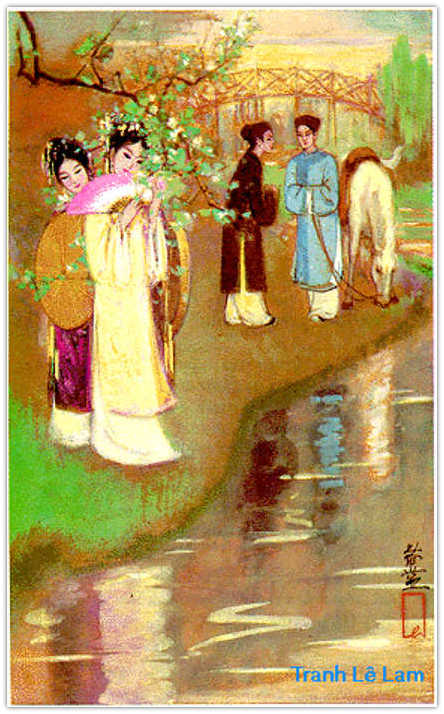
\includegraphics[scale=.25]{pdf/truyenkieu.jpg}  
\end{center}

\bl{Chàng Vương quen mặt ra chào}{\chàng \vương \quen \mặt \ra\chào}
\bl{Hai kiều e lệ nép vào dưới hoa}{\hai \Kiều \e\Lệ \nép \vào \dưới \hoa}
\newpage \setcounter{page}{16}
\hspace*{-1.75cm}\parbox{.65\textwidth}{\item \bl{Phong tư tài mạo tót vời}{\phongtư \tài \mạo \Tót \vời}
\item \bl{Vào trong phong nhã, ra ngoài hào hoa}{\vào \trong \PHong \nhã \ra\ngoài \Hào \hoa}
\item \bl{Chung quanh vẫn đất nước nhà}{\chung \quanh \vẫn \đất \nước \nhà}
\item \bl{Với Vương Quan trước vẫn là song thân}{\với \vương \QUan \trước \vẫn \là \SONG \THân}
\item \bl{Vẫn nghe thơm nức hương lân}{\vẫn \nghe \thơm \nức \hương \lân}
\item \bl{Một nền Đồng  tước khóa xuân hai Kiều}{\một \nền \đồngtước \Khóa \xuân \hai \KIều}
\item \bl{Nước non cách mấy buồng điều}{\nước \non \cách \mấy \buồng \ĐIều}
\item \bl{Những là trộm dấu thầm yêu chốc mòng}{ \những \là \Trộm \dấu \thầm  \yêu \chốc \mòng}
\item \bl{May thay giải cấu tương phùng}{\may \Thay \giải \Cấu \tương \phùng}
\item \bl{Gặp tuần đỏ lá thỏa lòng tìm hoa}{\gặp \tuần \đỏ \lá \thỏa \lòng \tìm \hoa}
}\Kieul{7.5}{008}\newpage 




\hspace*{-1.75cm}\parbox{.65\textwidth}{\item \bl{Bóng hồng nhác thấy nẻo xa}{ \bóng \hồng \nhác \thấy \nẻo \xa}
\item \bl{Xuân lan thu cúc mặn mà cả đôi}{\xuân \lan \thu \cúc \mặn \mà \cả \đôi}
\item \bl{Người quốc sắc kẻ thiên tài}{\người \quốc \sắc \kẻ \THIên \tài}
\item \bl{Tình trong như đã mặt ngoài còn e}{\tình \trong\như  \đã \mặt \ngoài \Còn \e}
\item \bl{Chập chờn cơn tỉnh cơn mê}{\chập \chờn \cơn \tỉnh \cơn \mê}
\item \bl{Rốn ngồi chẳng tiện dứt về chỉn khôn}{\Rốn \ngồi \chẳng \tiện \DỨt \về \chỉn \khôn}
\item \bl{Bóng tà như giục cơn buồn}{\bóng \tà\như  \giục \cơn \buồn}
\item \bl{Khách đà lên ngựa người còn ghé theo}{\khách \đà \lên \ngựa \người \Còn \ghé \theo}
\item \bl{Dưới cầu nước chảy trong veo}{\dưới \cầu  \nước \chảy \Trong \veo}
\item \bl{Bên cầu tơ liễu bóng chiều la tha}{\bên \cầu \tơ \liễu \bóng \chiều \latha}

}\kieur{009}\newpage 
\hspace*{-1.75cm}\parbox{.65\textwidth}{\item \bl{Kiều từ trở gót trướng hoa}{\kiều \từ  \trở \gót \trướng \hoa}
\item \bl{Mặt trời gác núi chiêng đà thu không}{\mặt \trời \GÁc \núi \chiêng \đà \Thu \không}
\item \bl{Mảnh trăng chênh chếch dòm song}{\mảnh \trăng \chênhchếch \dòm \SONG}
\item \bl{Vàng gieo ngấn nước cây lồng bóng sân}{\vàng \gieo \đáy \nước \cây \lồng \bóng \sân}
\item \bl{Hải đường rã ngọn đông lân}{\hải \Đường \rã \ngọn \đông \lân}
\item \bl{Giọt sương gieo nặng cành xuân la đà}{\giọt \sương \Gieo \nặng \cành \xuân \lađà}
\item \bl{Một mình lặng ngắm bóng nga}{\một \mình \lặng \ngắm \bóng \nga}
\item \bl{Rộn đường gần với nỗi xa bời bời}{\rộn \đường \gần \với \nỗi \xa \bời \bời}
\item \bl{Người mà đến thế thì thôi}{\người \mà \đến \thế  \thì \thôi}
\item \bl{Đời phồn hoa cũng là đời bỏ đi}{\đời \phồn \hoa \cũng \là \đời \bỏ \đi}

}\kieul{009}\newpage 
\hspace*{-1.75cm}\parbox{.65\textwidth}{\item \bl{Người đâu gặp gỡ làm chi}{\người \đâu \Gặpgỡ \làm \chi}
\item \bl{Trăm năm biết có duyên gì hay không}{\trăm \NĂM \biết \có \duyên \gì \hay \không}
\item \bl{Ngổn ngang trăm mối bên lòng}{\ngổn \ngang \trăm \mối \bên \lòng}
\item \bl{Nên câu tuyệt diệu ngụ trong tính tình}{\nên \câu \tuyệt \diệu \ngụ \trong \TÍnh \tình}
\item \bl{Chênh chênh bóng nguyệt xế mành}{\chênh \chênh \bóng \nguyệt \xế \mành}
\item \bl{Tựa nương bên triện một mình thiu thiu}{\tựa \Nương \bên \triện \một \mình \thiu \thiu}
\item \bl{Thoắt đâu thấy một tiểu kiều}{\thoắt \đâu \thấy \một \tiểu \Kiều }
\item \bl{Có chiều phong vận, có chiều thanh tân}{\có \chiều \PHong  \Vận \có \chiều \thanhtrong  \tân}
\item \bl{Sương in mặt tuyết pha thân}{\sương \in \mặt \tuyết \pha \thân }
\item \bl{Sen vàng lãng đãng như gần như xa}{\sen \vàng \lãng \đãng\như  \gần\như  \xa}


}\Kieur{6.75}{010}\newpage 
\hspace*{-1.75cm}\parbox{.65\textwidth}{\item \bl{Rước mừng đón hỏi dò la}{\rước \mừng \Đón \hỏi \dòla}
\item \bl{Đào nguyên lạc lối đâu mà đến đây}{\đàonguyên \lạc \lối \đâu \mà \đến \đây}
\item \bl{Thưa rằng: Thanh khí xưa nay}{\thưa \rằng \thanh \khí \xưanay}
\item \bl{Mới cùng nhau lúc ban ngày đã quên}{\mới \Cùng  \nhau \lúc \ban \ngày \đã \quên}
\item \bl{Hàn gia ở mé tây thiên}{\hàn \gia \ở \mé \tây \THIÊn}
\item \bl{Dưới dòng nước chảy bên trên có cầu}{\dưới \dòng \nước \chảy \bên \trên \có \cầu}
\item \bl{Mấy lòng hạ cố đến nhau}{\mấy \lòng \hạ \Cố \đến \nhau}
\item \bl{Mấy lời hạ tứ ném châu gieo vàng}{\mấy \Lời   \hạ \TỨ \ném \châu \gieo \vàng}
\item \bl{Vâng trình hội chủ xem tường}{\vâng \trình \hội \chủ \xem \Tường}
\item \bl{Mà sao trong sổ đoạn trường có tên}{\mà \SAO  \trong \sổ \Đoạntrường \có \tên}

}\Kieul{7}{010}\newpage 

\hspace*{-1.75cm}\parbox{.65\textwidth}{\item \bl{Âu đành quả kiếp nhân duyên}{\âu \đành \Quả \kiếp \nhânduyên}
\item \bl{Cùng người một hội một thuyền đâu xa}{\Cùng  \người \một \hội \một \thuyền \đâu \xa}
\item \bl{Này mười bài mới mới ra}{\này  \mười \bài \mới \mới \ra}
\item \bl{Câu thần lại mượn bút hoa vẽ vời}{\câu \thần \lại \mượn \bút \hoa \vẽ \vời}
\item \bl{Kiều vâng lĩnh ý đề bài}{\kiều \vâng \lĩnh \ý \Đề \bài}
\item \bl{Tay tiên một vẫy đủ mười khúc ngâm}{\tay \tiên \một \vẫy \đủ \mười \khúc \ngâm}
\item \bl{Xem thơ nấc nở khen thầm}{\xem \thơ \nấcnở \khen \thầm}
\item \bl{Giá đành tú khẩu cẩm tâm khác thường}{\giá  \đành \Tú \khẩu \cẩm \tâm \khác \thường}
\item \bl{Ví đem vào tập đoạn trường}{\ví \đem \vào \tập \đoạntrường}
\item \bl{Thì treo giải nhất chi nhường cho ai}{\thì \treo \giải \nhất \chi \nhường \cho \ai}

}\kieur{011}\newpage 

\hspace*{-1.75cm}\parbox{.65\textwidth}{\item \bl{Thềm hoa khách đã trở hài}{\thềm \hoa \khách \đã \Trở \hài}
\item \bl{Nàng còn cầm lại một hai tự tình}{\nàng \Còn \cầm \lại \một \hai \TỰ \tình}
\item \bl{Gió đâu khua bức mành mành}{\gió \đâu \khua \bức \mànhmành}
\item \bl{Tỉnh ra mới biết rằng mình chiêm bao}{\tỉnh \ra \mới \biết \rằng \mình \chiêm \bao}
\item \bl{Trông theo nào thấy đâu nào}{\trông \theo \nào  \thấy \đâu \nào }
\item \bl{Hương thừa dường hãy ra vào đâu đây}{\hương \thừa \dường \hãy \ra \vào \đâu \đây}
\item \bl{Một mình lưỡng lự canh chầy}{\một \mình \lượng \lự \canh \chầy}
\item \bl{Đường xa nghĩ nỗi sau này mà kinh}{\đường \xa \nghĩ \nỗi \sau \này  \mà \KINh}
\item \bl{Hoa trôi bèo giạt đã đành}{\hoa \trôi \bèo \giạt \đã \đành}
\item \bl{Biết duyên mình biết phận mình thế thôi}{\biết \duyên \mình \biết \phận \mình \thế  \thôi}

}\kieul{011}\newpage 

\hspace*{-1.75cm}\parbox{.65\textwidth}{\item \bl{Nỗi riêng lớp lớp sóng dồi}{\nỗi \riêng \lớp \lớp \sóng \dồi}
\item \bl{Nghĩ đòi cơn lại sụt sùi đòi cơn}{\nghĩ \đòi \cơn \lại \sụtsùi \đòi \cơn}
\item \bl{Giọng kiều rền rĩ trướng loan}{\Giọng \Kiều \rền \rĩ \trướng \loan}
\item \bl{Nhà huyên chợt tỉnh hỏi cơn cớ gì}{\nhà \Huyên \chợt \tỉnh \hỏi \cơn \cớ \gì}
\item \bl{Cớ sao trằn trọc canh khuya}{\cớ \SAO  \trằn \trọc \canh \khuya}
\item \bl{Màu hoa lê hãy đầm đìa giọt mưa}{\màu \hoa \lê \hãy \đầm \đìa \giọt \mưa}
\item \bl{Thưa rằng: Chút phận ngây thơ}{\thưa \rằng \chút \phận \ngâythơ}
\item \bl{Dưỡng sinh đôi nợ tóc tơ chưa đền}{\dưỡng \sinh \đôi \nợ \tóc \tơ \Chưa \đền}
\item \bl{Buổi ngày chơi mả Đạm Tiên}{\buổi \Ngày \chơi \mả \đạm \tiên}
\item \bl{Nhắp đi thoắt thấy ứng liền chiêm bao}{\nhắp \đi \thoắt \thấy \ứng \liền \chiêm \bao}

}\Kieur{6.5}{012}\newpage 

\hspace*{-1.75cm}\parbox{.65\textwidth}{\item \bl{Đoạn trường là sổ thế nào}{\đoạntrường \là \số \thếnào}
\item \bl{Bài ra thế ấy vịnh vào thế kia}{\bài \ra \thế  \ấy \vịnh \vào \thế  \kia}
\item \bl{Cứ trong mộng triệu mà suy}{\cứ \trong \mộng \triệu \mà \suy}
\item \bl{Thân con thôi có ra gì mai sau}{\thân  \con \thôi \có \ra \gì \Mai  \sau}
\item \bl{Dạy rằng: Mộng huyễn chắc đâu}{\dạy \rằng \mộng \huyễn \CHắc \đâu}
\item \bl{Bỗng không mua não chác sầu nghĩ nao}{\bỗng \không \Mua \não \chác \sầu \nghĩ \nao}
\item \bl{Vâng lời khuyên giải thấp cao}{\vâng \Lời   \khuyêngiải \thấpcao}
\item \bl{Chưa xong điều nghĩ lại  dào mạch Tương}{\chưa \xong \Điều   \nghĩ \lại \dào \Mạch \Tương}
\item \bl{Ngoài song thỏ thẻ oanh vàng}{\ngoài \SONG \thỏ \thẻ \oanh \vàng}
\item \bl{Nách tường bông liễu bay  sang láng giềng}{\nách \tường \bông \liễu \bay \sang \láng \Giềng}

}\Kieul{7.25}{012}\newpage 

\hspace*{-1.75cm}\parbox{.65\textwidth}{\item \bl{Hiên tà gác bóng nghiêng nghiêng}{\hiên \tà \Gác \bóng \nghiêng \nghiêng}
\item \bl{Nỗi riêng riêng chạnh tấc riêng một mình}{\nỗi \riêng \riêng \chạnh \tấc \riêng \một \mình}
\item \bl{Cho hay là giống hữu tình}{\cho \hay \là \giống \hữu \tình}
\item \bl{Đố ai gỡ mối tơ mành cho xong}{\đố \ai \gỡ \mối \tơ \Mành \cho \xong}
\item \bl{Chàng Kim từ lại thư song}{\chàng \kim \từ \lại \thư \SONG}
\item \bl{Nỗi nàng canh cánh bên lòng biếng khuây}{\nỗi \nàng \canh \Cánh \bên \lòng \biếng \khuây}
\item \bl{Sầu đong càng gạt càng đầy}{\sầu \Đong \càng \gạt \càng \đầy}
\item \bl{Ba thu dồn lại một ngày dài ghê}{\ba \thu \dồn \lại \một \ngày \dài \Ghê}
\item \bl{Mây Tần khóa kín song the}{\mây \tần \khóa \kín \SONG \THE}
\item \bl{Bóng hồng liệu nẻo đi về chiêm bao}{\bóng \hồng \liệu \nẻo \đi \về \chiêm \bao}

 }\kieur{013}\newpage 
\hspace*{-1.75cm}\parbox{.65\textwidth}{\item \bl{Tuần trăng khuyết đĩa dầu hao}{\tuần \trăng \khuyết \đĩa \dầu \hao}
\item \bl{Mặt tơ tưởng mặt lòng ngao ngán lòng}{\mặt \Tơ \tưởng \mặt \lòng \ngao \ngán \lòng}
\item \bl{Buồng văn hơi giá như đồng}{\buồng \văn \hơi \GIá \như   \ĐỒng}
\item \bl{Trúc se ngòi thỏ tơ chùng phím loan}{\trúc \se \ngòi \thỏ \tơ \chùng \phím \loan}
\item \bl{Mành tương phơn phớt gió đàn}{\mành \Tương \phơn \phớt  \gió \đàn}
\item \bl{Hương gây mùi nhớ trà khan giọng tình}{\hương \gây \mùi \nhớ \trà \khan \GIọng \tình}
\item \bl{Ví chăng duyên nợ ba sinh}{\ví \chăng \duyên \Nợ  \ba \sinh}
\item \bl{Cớ chi đem giống khuynh thành trêu ngươi}{\cớ \chi \đem \giống \khuynh \thành \trêu \ngươi}
\item \bl{Bâng khuâng nhớ cảnh nhớ người}{\bâng \khuâng \nhớ \cảnh \nhớ \người}
\item \bl{Nhớ nơi kỳ ngộ vội dời chân đi}{\nhớ \nơi \kỳ \ngộ \vội \dời \chân \đi}

}\kieul{013}\newpage 

\hspace*{-1.75cm}\parbox{.65\textwidth}{\item \bl{Một làn cỏ mọc xanh rì}{\một \làn \cỏ \mọc \xanh \rì}
\item \bl{Nước ngâm trong vắt thấy gì nữa đâu}{\nước \ngâm \Trong \vắt \thấy \gì \nữa \đâu}
\item \bl{Gió chiều như giục cơn sầu}{\gió \chiều\như  \gợi \cơn \sầu}
\item \bl{Bông lau hiu hắt như màu khơi trêu}{\bông \lau \hiuhắt\như   \màu \khơi \trêu}
\item \bl{Chạnh riêng tưởng ít tình nhiều}{\Chạnh \riêng \tưởng \ít \tình \nhiều}
\item \bl{Xăm xăm đè nẻo Lam  kiều lần sang}{\xăm \xăm \đè \nẻo \lam \ \KIỀu \lần \sang}
\item \bl{Thâm nghiêm kín cổng cao tường}{\Thâm \nghiêm \kín \cổng \Cao \tường}
\item \bl{Cạn dòng lá thắm dứt đường chim xanh}{\cạn \dòng \lá \thắm \dứt \đường \chim \xanh}
\item \bl{Lơ thơ tơ liễu buông mành}{\Lơthơ \tơ \liễu \buông \mành}
%{\lơthơsvg \tơ \liễu \buông \mành}
\item \bl{Con oanh học nói trên cành mỉa mai}{\con \oanh \học \nói \trên \cành \mỉa \MAi}

}\Kieur{6.5}{014}\newpage 
\hspace*{-1.75cm}\parbox{.65\textwidth}{\item \bl{Mấy lần cửa đóng then cài}{\mấy \lần \cửa  \đóng \then \cài}
\item \bl{Đầy thềm hoa rụng biết người ở đâu}{\đầy \thềm \hoa \rụng \biết \người \ở \đâu}
\item \bl{Tần ngần đứng suốt giờ lâu}{\tần \ngần \đứng \suốt \giờ \lâu}
\item \bl{Dạo quanh chợt thấy mái sau có nhà}{\dạo \quanh \chợt \thấy \mái \sau \có \nhà}
\item \bl{Là nhà Ngô Việt thương gia}{\là  \nhà \ngô \việt \thương \gia}
\item \bl{Buồng không để đó người xa chưa về}{\buồng \không \để \đó \người \xa \Chưa \về}
\item \bl{Lấy điều du học hỏi thuê}{\lấy \Điều  \du \học \hỏi \thuê}
\item \bl{Túi đàn cặp sách đề huề dọn sang}{\túi \đàn \cặp \sách \đề \huề \dọn \sang}
\item \bl{Có cây có đá sẵn sàng}{\có \cây \có \Đá \sẵn \sàng}
\item \bl{Có hiên Lãm  thúy nét vàng chưa phai}{\có \hiên \lãm  \thuý \nét \vàng \chưa \phai}

}\Kieul{7.5}{014}\newpage 

\hspace*{-1.75cm}\parbox{.65\textwidth}{\item \bl{Mừng thầm chốn ấy chữ bài}{\mừng \thầm \chốn \ấy \chữ \bài}
\item \bl{Ba sinh âu hẳn duyên trời chi đây}{\ba \sinh \âu \hẳn \duyên \trời \chi \đây}
\item \bl{Song hồ nửa khép cánh mây}{\SONG \hồ糊 \nửa \khép \cánh \mây}
\item \bl{Tường đông ghé mắt ngày ngày hằng trông}{\tường \đông \ghé \mắt \ngày \ngày \hằng \trông}
\item \bl{Tấc gang động khóa nguyên phong}{\tấc \gang \Động \khóa \Nguyên \Phong}
\item \bl{Tuyệt mù nào thấy bóng hồng vào ra}{\tuyệt \mù \nào  \thấy \bóng \hồng \vào \ra}
\item \bl{Nhẫn từ quán khách lân la}{\nhẫn \từ  \quán \khách \lânla}
\item \bl{Tuần trăng điểm đốt  nay đà thèm hai}{\tuần \trăng \điểm \Đốt \nay \đà \thèm \hai}
\item \bl{Cách tường phải buổi êm trời}{\cách \tường \phải \buổi \êm \trời}
\item \bl{Dưới đào dường có bóng người thướt tha}{\dưới \đào \dường \có \bóng \người \thướt \tha}

}\kieur{015}\newpage 

\hspace*{-1.75cm}\parbox{.65\textwidth}{\item \bl{Buông cầm xốc áo vội ra}{\buông \Cầm  \xốc \áo \vội \ra}
\item \bl{Hương còn thơm nức người đà vắng tanh}{\hương \Còn \thơm \nức \người \đà \vắng \tanh}
\item \bl{Lần theo tường gấm dạo quanh}{\lần \theo \tường \gấm \dạo \quanh}
\item \bl{Trên đào nhác thấy một cành kim thoa}{\trên \đào \nhác \thấy \một \cành \kim \Thoa}
\item \bl{Giơ tay với lấy về nhà}{\giơ \tay \Với \lấy \về \nhà}
\item \bl{Này trong khuê các đâu mà đến đây}{\này  \trong \khuê \các \đâu \mà \đến \đây}
\item \bl{Ngẫm âu người ấy báu này}{\ngẫm \âu \người \ấy \báu \này }
\item \bl{Chẳng duyên chưa dễ vào tay ai cầm}{\chẳng \duyên \Chưa \dễ \vào \tay \ai \cầm}
\item \bl{Liền tay ngắm nghía biếng nằm}{\liền \tay \ngắm \nghía \biếng \Nằm}
\item \bl{Hãy còn thoang thoảng hương trầm chưa phai}{\hãy \Còn \thoang \thoảng \hương \trầm \Chưa \phai}

}\kieul{015}\newpage 
\hspace*{-1.75cm}\parbox{.65\textwidth}{\item \bl{Tan sương đã thấy bóng người}{\tan \sương \đã \thấy \bóng \người}
\item \bl{Quanh tường ra ý tìm tòi ngẩn ngơ}{\quanh \tường \ra \ý \tìm \tòi \ngẩn \ngơ}
\item \bl{Sinh đà có ý đợi chờ}{\sinh \đà \có \ý \đợi \chờ}
\item \bl{Cách tường lên tiếng xa đưa ướm lòng}{\cách \tường \lên \tiếng \xa \đưa \ướm \lòng}
\item \bl{Thoa này bắt được hư không}{\Thoa \này  \bắt \được \hư \không}
\item \bl{Biết đâu Hợp  phố mà mong châu về}{\biết \đâu \hợp \ \phố \mà \mong \châu \về}
\item \bl{Tiếng Kiều nghe lọt bên kia}{\tiếng \kiều \nghe \lọt \bên \kia}
\item \bl{Ơn lòng quân tử sá gì của rơi}{\ơn \lòng \quântử \Sá \gì \của \rơi}
\item \bl{Chiếc thoa nào của mấy mươi}{\chiếc \Thoa \nào  \của \mấy \mươi}
\item \bl{Mà lòng trọng nghĩa khinh tài xiết bao}{\mà \lòng \trọngnghĩakhinhtài \Xiết \bao}

}\kieurr{016}\newpage  

\hspace*{-1.75cm}\parbox{.65\textwidth}{\item \bl{Sinh rằng: Lân lý ra vào}{\sinh \rằng \lân \Lý \ra \vào}
\item \bl{Gần đây nào phải người nào xa xôi}{\gần \đây \nào  \phải \người \nào  \xaxôi}
\item \bl{Được rày nhờ chút thơm rơi}{\được \rày \nhờ \chút \thơm \rơi}
\item \bl{Kể đà thiểu não lòng người bấy nay}{\kể \đà \thiểu \não \lòng \người \bấy \nay}
\item \bl{Mấy lâu mới được một ngày}{\mấy \lâu \mới \được \một \ngày}
\item \bl{Dừng chân gạn chút niềm tây gọi là}{\Dừng \chân \GẠn \chút \niềm \tây \gọi \là}
\item \bl{Vội về thêm lấy của nhà}{\vội \về \thêm \lấy \của \nhà}
\item \bl{Xuyến vàng đôi chiếc khăn là một vuông}{\xuyến \vàng \đôi \chiếc \khăn \làsvg \một \vuông}
\item \bl{Bậc mây rón bước ngọn tường}{\bậc \mây \rón \bước \ngọn \tường}
\item \bl{Phải người hôm nọ rõ ràng chẳng nhe}{\phải \người \hôm \nọ \rõ \ràng \Chẳng \nhe}

}\kieull{016}\newpage 



\hspace*{-1.75cm}\parbox{.65\textwidth}{\item \bl{Sượng sùng giữ ý rụt dè}{\sượng \sùng \giữ \ý \rụt \dè}
\item \bl{Kẻ nhìn rạng mặt người e cúi đầu}{\kẻ \nhìn \Rạng \mặt \người \e \cúi \Đầu}
\item \bl{Rằng: Từ ngẫu nhĩ gặp nhau}{\rằng \từ  \ngẫu \nhĩ \gặp \nhau}
\item \bl{Thầm trông trộm nhớ bấy lâu đã chồn}{\thầm \trông \Trộm \nhớ \Bấylâu \đã \chồn}
\item \bl{Xương mai tính đã thâu mòn}{\xương \mai \tính \đã \thâu \mòn}
\item \bl{Lần lừa ai biết hãy còn hôm nay}{\lần \lừa \ai \biết \hãy \Còn \hômnay}
\item \bl{Tháng tròn như gởi cung mây}{\tháng \Tròn\như  \gởi \cung \mây}
\item \bl{Trần trần một phận ấp cây đã liều}{\Trần \Trần \một \phận \ấp \cây \đã \liều}
\item \bl{Tiện đây xin một hai điều}{\tiện \đây \xin \một \hai \Điều }
\item \bl{Đài gương soi đến dấu bèo cho chăng}{\đài \gương \soi \đến \dấu \bèo \cho \chăng}

}\kieur{017}\newpage 

\hspace*{-1.75cm}\parbox{.65\textwidth}{\item \bl{Ngần ngừ nàng mới thưa rằng}{\ngần \ngừ \nàng \mới \thưa \rằng}
\item \bl{Thói nhà băng tuyết chất hằng phỉ phong}{\thói \nhà \băng \tuyết \chất \hằng \phỉphong}
\item \bl{Dù khi lá thắm chỉ hồng}{\dù \khi \lá \thắm\CHỈ \hồng}
\item \bl{Nên chăng thì cũng tại lòng mẹ cha}{\nên \chăng \thì \cũng \tại \lòng \mẹ \cha}
\item \bl{Nặng lòng xót liễu vì hoa}{\nặng \lòng \xót \liễu \vì \hoa}
\item \bl{Trẻ thơ đã biết đâu mà dám thưa}{\trẻthơ \đã \biết \đâu \mà \dám \thưa}
\item \bl{Sinh rằng: Rày gió mai mưa}{\sinh \rằng \rày \gió \Mai  \mưa}
\item \bl{Ngày xuân đã dễ tình cờ mấy khi}{\ngày \xuân \đã \dễ \tình \CỜ \mấy \khi}
\item \bl{Dù chăng xét tấm tình si}{\dù \chăng \xét \tấm \tìnhsi}
\item \bl{Thiệt đây mà có ích gì đến ai}{\thiệt \đây \mà \có \ích \gì \đến \ai}

}\kieul{017}\newpage 

\hspace*{-1.75cm}\parbox{.65\textwidth}{\item \bl{Chút chi gắn bó một hai}{\chút \chi \gắn \Bó  \một \hai}
\item \bl{Cho đành rồi sẽ liệu bài mối manh}{\cho \đành \rồi \sẽ \liệu \bài \mối \manh}
\item \bl{Khuôn thiêng dù phụ tấc thành}{\khuôn \thiêng \dù \Phụ \tấc \Thành}
\item \bl{Cũng liều bỏ quá xuân xanh một đời}{\cũng \liều \bỏ \quá \xuân \xanh \một \đời}
\item \bl{Lượng xuân dù quyết hẹp hòi}{\lượng \xuân \dù \quyết \hẹp \hòi}
\item \bl{Công đeo đuổi chẳng thiệt thòi lắm ru}{\công \đeođuổi \chẳng \thiệt \thòi \lắm \Ru}
\item \bl{Lặng nghe lời nói như ru}{\Lặng \nghe \Lời   \nói\như  \ru}
\item \bl{Chiều xuân dễ khiến nét thu ngại ngùng}{\chiều \xuân \dễ \khiến \nét \thu \ngạingùng}
\item \bl{rằng: Trong buổi mới lạ lùng}{\rằng \trong \buổi \mới \lạ \lùng}
\item \bl{Nể lòng có nhẽ cầm lòng cho đang}{\nể \lòng \có \nhẽ \cầm \lòng \cho \đang}
}\kieurr{018}\newpage 

\hspace*{-1.75cm}\parbox{.65\textwidth}{\item \bl{Đã lòng quân tử đa mang}{\đã \lòng \quântử \đa\mang}
\item \bl{Một lời vâng tạc đá vàng thuỷ chung}{\một \Lời   \vâng \Tạc \Đá \vàng \thuỷchung}
\item \bl{Được lời như cởi tấm lòng}{\được \Lời  \như  \Cởi \tấm \lòng}
\item \bl{Giở kim thoa với khăn hồng trao tay}{\Giở \kim \Thoa \với \khăn \hồng \trao \tay}
\item \bl{Rằng: Trăm năm cũng từ đây}{\rằng \trăm \NĂM \cũng \từ  \đây}
\item \bl{Của tin gọi một chút này làm ghi}{\của \tin  \gọi \một \chút \này  \làm \ghi}
\item \bl{Sẵn tay khăn gấm quạt quỳ}{\sẵn \tay \khăn \gấm \quạt \Quỳ}
\item \bl{Với cành thoa ấy tức thì đổi trao}{\với \cành \Thoa \ấy \tứcthì \đổi \trao}
\item \bl{Một lời vừa gắn tất giao}{\một \Lời   \vừa \gắn \tấtgiao}
\item \bl{Mái sau dường có xôn xao tiếng người}{\mái \sau \dường \có \xôn \xao \tiếng \người}

}\kieull{018}\newpage 

\hspace*{-1.75cm}\parbox{.65\textwidth}{\item \bl{Vội vàng lá rụng hoa rơi}{\vộivàng \lá \rụng \hoa \rơi}
\item \bl{Chàng về viện sách nàng dời lầu trang}{\chàng \về \viện \sách \nàng \dời \Lầu \Trang}
\item \bl{Từ phen đá biết tuổi vàng}{\từ \phen \Đá \biết \tuổi \vàng}
\item \bl{Tình càng thấm thía dạ càng ngẩn ngơ}{\tình \càng \thấmthía \Dạ \càng \ngẩnngơ}
\item \bl{Sông Tương một dải nông sờ}{\sông \Tương \một \Dải \nông \sờ}
\item \bl{Bên trông đầu nọ bên chờ cuối kia}{\bên \trông \Đầu  \nọ \bên \chờ \cuối \kia}
\item \bl{Một tường tuyết trở sương che}{\một \tường \tuyết \Trở \sương \che}
\item \bl{Tin xuân đâu dễ đi về cho năng}{\tin  \xuân \đâu \dễ \đi \về \cho \năng}
\item \bl{Lần lần ngày gió đêm trăng}{\lần \lần \ngày \gió \đêm \trăng}
\item \bl{Thưa hồng rậm lục đã chừng xuân qua}{\Thưa \hồng \rậm \lục \đã \chừng \xuân \qua}

}\kieur{019}\newpage 

\hspace*{-1.75cm}\parbox{.65\textwidth}{\item \bl{Vừa ngày sinh nhật ngoại gia}{\vừa \ngày \sinh \nhật \ngoại \gia}
\item \bl{Trên song đường dưới nữa là hai em}{\trên \song \Đường \dưới \nữa \là  \hai \em}
\item \bl{Tưng bừng sắm sửa áo xiêm}{\tưng \bừng \sắm \sửa \áo \xiêm}
\item \bl{Cần dâng một lễ xa đem tấc thành}{\Cần \dâng \một \lễ \xa \đem \tấc \Thành}
\item \bl{Nhà lan thanh  vắng một mình}{\nhà \lan \Thanh \vắng \một \mình}
\item \bl{Ngẫm cơ hội ngộ đã đành hôm nay}{\ngẫm \CƠ \hội \ngộ \đã \đành \hômnay}
\item \bl{Thời trân thức thức sẵn bày}{\thời \trân \thức \thức \sẵn \bày}
\item \bl{Gót sen thoăn thoắt dạo ngay mái tường}{\gót \sen \thoăn \thoắt \dạo \ngay  \mái \tường}
\item \bl{Cách hoa sẽ dặng tiếng vàng}{\cách \hoa \sẽ \dặng \tiếng \vàng}
\item \bl{Dưới hoa thấy đã  có chàng đứng mong}{\dưới \hoa \thấy \đã \có \chàng \đứng \mong}
}\kieul{019}\newpage 


\hspace*{-1.75cm}\parbox{.65\textwidth}{\item \bl{Trách lòng hờ hững với lòng}{\trách \lòng \hờ \hững \với \lòng}
\item \bl{Lửa hương chốc để lạnh lùng bấy lâu}{\lửa \hương \chốc \để \lạnh \lùng \Bấylâu}
\item \bl{Những là đắp nhớ đổi sầu}{\những \là  \đắp \nhớ \đổi \sầu}
\item \bl{Tuyết sương nhuốm nửa mái đầu hoa râm}{\tuyết \sương \nhuốm \nửa \mái \Đầu  \hoa \râm}
\item \bl{Nàng rằng: Gió bắt mưa cầm}{\nàng \rằng \gió \bắt \mưa \cầm}
\item \bl{Đã cam tệ với tri âm bấy chầy}{\đã \cam \tệ \với \triâm \bấy \chầy}
\item \bl{Vắng nhà được buổi hôm nay}{\vắng \nhà \được \buổi \hômnay}
\item \bl{Lấy lòng gọi chút ra đây tạ lòng}{\lấy \lòng \gọi \chút \ra \đây \tạ \lòng}
\item \bl{Lần theo núi giả đi vòng}{\lần \theo \núi \giả \đi \vòng}
\item \bl{Cuối tường dường có nẻo thông mới rào}{\cuối \tường \dường \có \nẻo \THông \mới \rào}

}\kieurr{020}\newpage 

\hspace*{-1.75cm}\parbox{.65\textwidth}{\item \bl{Sấn tay mở khóa động đào}{\Sấn \tay \mở \khóa \Động \đào}
\item \bl{Rẽ mây trông rõ lối vào Thiên  thai}{\Rẽ\mây \trông \rõ \lối \vào \THIên \thai}
\item \bl{Càng nhìn mặt càng thêm tươi}{\càng \nhìn \mặt \càng \thêm \tươi}
\item \bl{Bên lời vạn phúc bên lời hàn huyên}{\bên \Lời  \vạn \phúc \bên \Lời  \hàn \huyên}
\item \bl{Sánh vai về chốn thư hiên}{\Sánh \vai \về \chốn \thư \hiên}
\item \bl{Góp lời phong nguyệt nặng nguyền non sông}{\góp \Lời   \PHong \nguyệt \nặng \nguyền \non \sông}
\item \bl{Trên yên bút giá thi đồng}{\trên \Yên \bút \Giá  \thiđồng}
\item \bl{Đạm thanh một bức tranh tùng treo trên}{\đạm \Thanh \một \bức \tranh \tùng \treo \Trên}
\item \bl{Phong sương được vẻ thiên nhiên}{\PHong \sương \được \vẻ \THIên \nhiên}
\item \bl{Mặn khen nét bút càng nhìn càng tươi}{\mặn \khen \nét \bút \càng \nhìn \càng \tươi}

}\kieull{020}\newpage 


\hspace*{-1.75cm}\parbox{.65\textwidth}{\item \bl{Sinh rằng: Phác họa vừa rồi}{\sinh \rằng \phác \HỌA  \vừa \rồi}
\item \bl{Phẩm đề xin một vài lời thêm hoa}{\phẩm \Đề \xin \một \vài \Lời   \thêm \hoa}
\item \bl{Tay tiên gió táp mưa sa}{\tay \tiên \gió \táp \mưa \sa}
\item \bl{Khoảng trên dừng bút thảo và bốn câu}{\khoảng \trên \Dừng \bút \thảo \và \bốn \câu}
\item \bl{Khen tài nhả ngọc phun châu}{\khen \tài \nhả \ngọc \phun \châu}
\item \bl{Nàng Ban ả Tạ cũng đâu có vầy}{\nàng \ban \ả \tạ \cũng \đâu\Có \vầy}
\item \bl{Kiếp tu xưa ví chưa dầy}{\kiếp \Tu \xưa \ví \chưa \Dầy}
\item \bl{Phúc nào nhắc được giá này cho ngang}{\phúc \nào  \nhắc \được \giá  \này  \cho \ngang}
\item \bl{Nàng rằng: Trộm liếc dung quang}{\nàng \rằng \trộm \Liếc \Dung \quang}
\item \bl{Chẳng sân ngọc bội cũng phường kim môn}{\chẳng \sân \ngọc \Bội \cũng \phường \kim \Môn}

}\kieur{021}\newpage 


\hspace*{-1.75cm}\parbox{.65\textwidth}{\item \bl{Nghĩ mình phận mỏng cánh chuồn}{\nghĩ \mình \phận \Mỏng \cánh \chuồn}
\item \bl{Khuôn xanh biết có vuông tròn mà hay}{\khuôn \xanh \biết \có \vuông \Tròn \mà \hay}
\item \bl{Nhớ từ năm hãy thơ ngây}{\nhớ \từ  \NĂM \hãy \thơngây}
\item \bl{Cứ trong tướng pháp lắm thầy chê bai}{\cứ \trong \Tướng \pháp \lắm \thầy \chêbai}
\item \bl{Anh hoa phát tiết ra ngoài}{\ANH \hoa \phát \tiết \ra \ngoài}
\item \bl{Nghìn thu bạc mệnh một đời tài hoa}{\nghìn \thu \bạcmệnh \một \đời \tài \hoa}
\item \bl{Trông người lại ngắm vào ta}{\trông \người \lại \ngắm \vào \ta}
\item \bl{Một dầy một mỏng biết là có nên}{\một \dầy \một \Mỏng \biết \là \có \nên}
\item \bl{Sinh rằng: Giải cấu là duyên}{\sinh \rằng \giải \Cấu \là \duyên}
\item \bl{Xưa nay nhân định thắng thiên cũng nhiều}{\xưanay \nhân \định \thắng \THIên \cũng \nhiều}
}\kieul{021}\newpage 


\hspace*{-1.75cm}\parbox{.65\textwidth}{\item \bl{Ví dù giải kết đến điều}{\ví \dù \Giải \kết \đến \Điều }
\item \bl{Thì đem vàng đá mà liều cho  thân}{\thì \đem \vàng \Đá \mà \liều \cho \thân }
\item \bl{Đủ điều trung khúc ân cần}{\đủ \Điều \TRung \khúc \âncần}
\item \bl{Lòng xuân phơi phới chén xuân tàng tàng}{\lòng \xuân \phới \phới \chén \xuân \tàng \tàng}
\item \bl{Ngày vui vắn chẳng đầy gang}{\ngày \vui \vắn \chẳng \đầy \gang}
\item \bl{Trông ra ác đã ngậm gương non đoài}{\trông \ra  \Ác \đã \Ngậm \gương \non \đoài}
\item \bl{Vắng nhà chẳng tiện ngồi dai}{\vắng \nhà \chẳng \tiện \ngồi \dai}
\item \bl{Giã chàng nàng mới kíp dời song sa}{\Giã \chàng \nàng \mới \kíp \dời \SOng \Sa}
\item \bl{Đến nhà vừa thấy tin nhà}{\đến \nhà \vừa \thấy \tin  \nhà}
\item \bl{Hai thân còn dở tiệc hoa chưa về}{\hai \THân \Còn \Dở \tiệc \hoa \Chưa \về}
}\kieurr{022}\newpage 


\hspace*{-1.75cm}\parbox{.65\textwidth}{\item \bl{Cửa ngoài vội rủ rèm the}{\cửa  \ngoài  \vội  \rủ  \rèm  \THE}
\item \bl{Xăm xăm băng nẻo vườn khuya một mình}{\xăm \xăm \Băng \nẻo \vườn \khuya \một \mình}
\item \bl{Nhặt thưa gương giọi đầu cành}{\Nhặt \thưa \gương \giọi \Đầu  \cành}
\item \bl{Ngọn đèn trông lọt trướng bình hắt hiu}{\ngọn \đèn \trông \lọt \trướng \BÌNh \hắt \hiu}
\item \bl{Sinh còn tựa án thiu thiu}{\sinh \Còn  \tựa \án \thiu \thiu}
\item \bl{Dở chiều như tỉnh dở chiều như mê}{\Dở \chiều\như  \tỉnh \Dở \chiều\như  \mê}
\item \bl{Tiếng sen sẽ động giấc hòe}{\tiếng \sen \sẽ \động \giấc \hòe}
\item \bl{Bóng trăng đã xế hoa lê lại gần}{\bóng \trăng \đã \xế \hoa \lê \lại \gần}
\item \bl{Bâng khuâng đỉnh Giáp non Thần}{\bângkhuâng \đỉnh \GIÁP \non \thần}
\item \bl{Còn ngờ giấc mộng đêm xuân mơ màng}{\Còn \NGỜ\giấc \mộng \đêm \xuân \mơ \màng}
}\kieull{022}\newpage

\hspace*{-1.75cm}\parbox{.65\textwidth}{\item \bl{Nàng rằng: Khoảng vắng đêm trường}{\nàng \rằng \khoảng \vắng \đêm \TRường}
\item \bl{Vì hoa nên phải đánh đường tìm hoa}{\vì \hoa \nên \phải \đánh \đường \tìm \hoa}
\item \bl{Bây giờ rõ mặt đôi ta}{\bâygiờ \rõ \mặt \đôi \ta}
\item \bl{Biết đâu rồi nữa chẳng là chiêm bao}{\biết \đâu \rồi \nữa \chẳng \là  \chiêm \bao}
\item \bl{Vội mừng làm lễ rước vào}{\vội \mừng \làm \lễ \rước \vào}
\item \bl{Đài sen nối sáp song đào thêm hương}{\đài \sen \NỐi \sáp \SOng \đào \thêm \hương}
\item \bl{Tiên thề cùng thảo một chương}{\TIÊn \thề \Cùng  \thảo \một \chương}
\item \bl{Tóc mây một món dao vàng chia đôi}{\tóc \mây \một \món \dao \vàng \chia \đôi}
\item \bl{Vầng trăng vằng vặc giữa trời}{\vầng \trăng \vằng \vặc \giữa \trời}
\item \bl{Đinh ninh hai mặt một lời song song}{\đinh \ninh \hai \mặt \một \Lời   \song  \song }
}\kieur{023}\newpage
\hspace*{-1.75cm}\parbox{.65\textwidth}{\item \bl{Tóc tơ căn vặn tấc lòng}{\tóc \tơ \căn \vặn \tấc \lòng}
\item \bl{Trăm năm tạc một chữ đồng đến xương}{\trăm \NĂM \Tạc \một \Chữ \Đồng \đến \xương}
\item \bl{Chén hà sánh giọng quỳnh tương}{\chén \Hà \Sánh \GIọng \quỳnhtương}
\item \bl{Dải là hương lộn bình gương bóng lồng}{\DẢI \LÀ  \hương \lộn \BÌNh \gương \bóng \lồng}
\item \bl{Sinh rằng: Gió mát trăng trong}{\sinh \rằng \gió \mát \trăng \Trong}
\item \bl{Bấy lâu nay một chút lòng chưa cam}{\Bấylâu \NAY \một \chút \lòng \chưa \cam}
\item \bl{Chày sương chưa nện cầu Lam}{\chày \sương \chưa \nện \cầu \lam}
\item \bl{Sợ lần khân quá ra sàm sỡ chăng}{\sợ \lần \khân \quá \ra \sàm \sỡ \chăng}
\item \bl{Nàng rằng: Hồng diệp xích thằng}{\nàng \rằng \hồng \diệp \xíchthằng}
\item \bl{Một lời cũng đã tiếng rằng: tương tri}{\một \Lời   \cũng \đã \tiếng \rằng \tươngtri}
}\kieul{023}\newpage 
\hspace*{-1.75cm}\parbox{.65\textwidth}{\item \bl{Xin điều nguyệt nọ hoa kia}{\xin \Điều  \nguyệt \nọ \hoa \kia}
\item \bl{Ngoài ra ai lại tiếc gì với ai}{\ngoài \ra \ai \lại \tiếc \gì \với \ai}
\item \bl{rằng: Nghe nổi tiếng cầm đài}{\rằng \nghe \nổi \tiếng \Cầm  \đài}
\item \bl{Nước non luống những lắng tai Chung Kỳ}{\nước \non \luống \những \lắng \Tai \Chung  \KỲ}
\item \bl{Thưa rằng: Tiện kỹ sá chi}{\thưa \rằng \Tiện \kỹ \Sá \chi}
\item \bl{Đã lòng dạy đến dạy thì phải vâng}{\đã \lòng \dạy \đến \dạy \thì \phải \vâng}
\item \bl{Hiên sau treo sẵn cầm trăng}{\hiên \sau \treo \sẵn \Cầm  \trăng}
\item \bl{Vội vàng sinh đã tay nâng ngang mày}{\vộivàng \sinh \đã \tay \nâng \ngang \mày }
\item \bl{Nàng rằng: Nghề mọn riêng tây}{\nàng \rằng \nghề \mọn \riêng \tây}
\item \bl{Làm chi cho nặng lòng này lắm thân}{\làm \chi \cho \nặng  \lòng \này  \lắm \Thân}
}\kieurr{024}\newpage 

\hspace*{-1.75cm}\parbox{.65\textwidth}{\item \bl{Lựa dần dây vũ dây văn}{\lựa \dần \dây \vũ \dây \văn}
\item \bl{Bốn dây to nhỏ theo vần cung thương}{\bốn \dây \to \nhỏ \theo \Vần \cung \thương}
\item \bl{Khúc đâu Hán Sở chiến trường}{\khúc \đâu \hán \Sở \chiến \trường}
\item \bl{Nghe ra tiếng sắt tiếng vàng chen nhau}{\nghe \ra \tiếng \Sắt \tiếng \vàng \Chen \nhau}
\item \bl{Khúc đâu Tư mã  Phượng cầu}{\khúc \đâu \tưmã  \phượng \Cầu}
\item \bl{Nghe ra như oán như sầu phải chăng}{\nghe \ra \như  \oán\như  \sầu \phải \chăng}
\item \bl{Kê Khang này khúc Quảng lăng}{\kê \khang \này  \khúc \quảng \lăng}
\item \bl{Một rằng hoa nhạc một rằng quy vân}{\một \rằng \Hoa \NHạc \một \rằng \quy \vân}
\item \bl{Quá quan này khúc Chiêu Quân}{\quá \QUAN \này  \khúc \chiêu \QUân}
\item \bl{Nửa phần luyến chúa nửa phần tư gia}{\nửa \phần \luyến \chúa \nửa \phần \tư \gia}

}\kieull{024}\newpage 


\hspace*{-1.75cm}\parbox{.65\textwidth}{\item \bl{Trong như tiếng hạc bay qua}{\Trong\như  \tiếng \hạc \bay \qua}
\item \bl{Đục như nước suối mới sa nửa vời}{\đục\như  \nước \suối \mới \sa \nửa \vời}
\item \bl{Tiếng khoan như gió thoảng ngoài}{\tiếng \khoan\như  \gió \thoảng \ngoài}
\item \bl{Tiếng mau rầm rập như trời đổ mưa}{\tiếng \Mau \rầmrập\như  \trời \đổ \mưa}
\item \bl{Ngọn đèn khi tỏ khi mờ}{\ngọn \đèn \khi \Tỏ \khi \mờ}
\item \bl{Khiến người ngồi đó cũng ngơ ngẩn sầu}{\khiến \người \ngồi \đó \cũng \ngơngẩn \sầu}
\item \bl{Khi tựa gối khi cúi đầu}{\khi \tựa \gối \khi \cúi \Đầu }
\item \bl{Khi vò chín khúc khi chau đôi mày}{\khi \Vò \chín \khúc \khi \Chau \đôi \Mày}
\item \bl{Rằng: Hay thì thật là hay}{\rằng  \hay \thì \thật \là  \hay}
\item \bl{Nghe ra ngậm đắng nuốt cay thế nào}{\nghe \ra \ngậm \Đắng \nuốt \cay \thếnào}

}\kieur{025}\newpage 

\hspace*{-1.75cm}\parbox{.65\textwidth}{\item \bl{Lựa chi những bậc tiêu tao}{\lựa \chi \những \bậc \tiêutao}
\item \bl{Dột lòng mình cũng nao nao lòng người}{\dột \lòng \mình \cũng \nao \nao \lòng \người}
\item \bl{Rằng: Quen mất nết đi rồi}{\rằng  \quen \mất \nết \đi \rồi}
\item \bl{Tẻ vui thôi cũng tính trời biết sao}{\tẻ \vui \thôi \cũng \TÍnh \trời \biết \SAO }
\item \bl{Lời vàng vâng lĩnh ý cao}{\Lời   \vàng \vâng \lĩnh \ý \Cao}
\item \bl{Họa dần dần bớt chút nào được không}{\hoạ  \dần \dần \bớt \chút \nào  \được \không}
\item \bl{Ngọn lan càng tỏ thức hồng}{\ngọn \lan \càng \Tỏ \thức \hồng}
\item \bl{Đầu mày cuối mắt càng nồng tấm yêu}{\Đầu  \mày  \cuối \mắt \càng \nồng \tấm \yêu}
\item \bl{Sóng tình dường đã xiêu xiêu}{\sóng \tình \dường \đã \xiêu \xiêu}
\item \bl{Xem trong âu yếm có chiều lả lơi}{\xem \trong \âu \yếm \có \chiều \lảlơi}

}\kieul{025}\newpage 

\hspace*{-1.75cm}\parbox{.65\textwidth}{\item \bl{Thưa rằng: Đừng lấy làm chơi}{\thưa \rằng  \đừng \lấy \làm \chơi}
\item \bl{Để cho thưa hết một lời đã nao}{\để  \cho \thưa \hết \một \Lời   \đã \nao}
\item \bl{Vẻ gì một đóa yêu đào}{\vẻ \gì \một \đóa \yêu \đào}
\item \bl{Vườn hồng chi dám ngăn rào chim xanh}{\vườn \hồng \chi \Dám \ngăn \rào \chim \xanh}
\item \bl{Đã cho vào bậc bố kinh}{\đã \cho \vào \bậc \bố \KInh}
\item \bl{Đạo tòng phu lấy chữ trinh làm đầu}{\đạo \tòng \phu \lấy \Chữ \trinh  \làm \Đầu }
\item \bl{Ra tuồng trên bộc trong dâu}{\ra \tuồng \trên \bộc \trong \dâu}
\item \bl{Những con người ấy ai cầu làm chi}{\những \con \người \ấy \ai \Cầu \làm \chi}
\item \bl{Phải điều ăn xổi ở thì}{\phải \Điều \ăn \xổi \ở \thì}
\item \bl{Tiết trăm năm nỡ bỏ đi một ngày}{\Tiết \trăm \NĂM \nỡ \bỏ \đi \một \ngày}

}\kieurr{026}\newpage 

\hspace*{-1.75cm}\parbox{.65\textwidth}{
\item \bl{Ngẫm duyên kỳ ngộ xưa nay}{\ngẫm \duyên \kỳ \ngộ \xưanay}
\item \bl{Lứa đôi ai lại đẹp tày Thôi Trương}{\lứa \đôi \ai \lại \đẹp \tày\Thôi \trương}
\item \bl{Mây mưa đánh đổ đá vàng}{\mây \mưa \đánh \Đổ \Đá \vàng}
\item \bl{Quá chiều trước đã chán chường yến anh}{\quá \chiều \trước \đã \chán \chường \yếnAnh}
\item \bl{Trong khi chắp cánh liền cành}{\trong \khi \Chắp \cánh \liền \cành}
\item \bl{Mà lòng rẻ rúng đã dành một bên}{\mà \lòng \rẻ \rúng \đã \DÀnh \một \bên}
\item \bl{Mái tây để lạnh hương nguyền}{\mái \tây \để \lạnh \hương \nguyền}
\item \bl{Xui duyên đằm thắm ra duyên bẻ bàng}{\xui \duyên \đằm \thắm \ra \duyên \bẽbàng}
\item \bl{Gieo thoi trước chẳng giữ ràng}{\gieo \thoi \trước \chẳng \giữ   \RÀng}
\item \bl{Để sau nên thẹn cùng chàng bởi ai}{\để \sau \nên \thẹn \Cùng  \chàng \Bởi \ai}

}\kieull{026}\newpage  


\hspace*{-1.75cm}\parbox{.65\textwidth}{
\item \bl{Vội gì liễu ép hoa nài}{\vội \gì \liễu \Ép \hoa \nài}
\item \bl{Còn thân còn một đền bồi có khi}{\Còn  \thân  \Còn   \một \đền \bồi \có \khi}
\item \bl{Thấy lời đoan chính dễ nghe}{\thấy \Lời   \đoan \chính \dễ \nghe}
\item \bl{Chàng càng thêm nể thêm vì mười phân}{\chàng \càng \thêm \nể \thêm \vì \mười \phân}
\item \bl{Bóng tàu vừa lạt vẻ ngân}{\bóng \tàu \vừa \lạt \vẻ \ngân}
\item \bl{Tin đâu đã gõ cửa ngăn gọi vào}{\Tin   \đâu \đã \gõ \cửa  \ngăn \gọi \vào}
\item \bl{Nàng thì vội trở buồng thêu}{\nàng \thì \vội \Trở \buồng \thêu}
\item \bl{Sinh thì dạo gót sân đào bước ra}{\sinh \thì \dạo \gót \sân \đào \bước \ra}
\item \bl{Cửa ngoài vừa ngỏ then hoa}{\cửa \ngoài \vừa \ngỏ \then \hoa}
\item \bl{Gia đồng vào gửi thư nhà mới sang}{\giađồng \vào \gửi \thư \nhà \mới \sang}
}\kieur{027}\newpage 
\hspace*{-1.75cm}\parbox{.65\textwidth}{
\item \bl{Mở xem thủ bút nghiêm đường}{\mở \xem \Thủ \bút \nghiêm \Đường}
\item \bl{Nhắn rằng: thúc phụ xa đường mệnh chung}{\nhắn \rằng \Thúc \phụ \xa \đường \mệnh \chung}
\item \bl{Hãy còn ký táng liêu đông}{\hãy \Còn  \ký \Táng \liêu \đông}
\item \bl{Cố hương khơi diễn ngàn trùng sơn khê}{\cố \Hương \Khơi \diễn \ngàn \trùng \sơn \khê}
\item \bl{Rày đưa linh sấn về quê}{\rày \đưa \linh \sấn \về \quê }
\item \bl{Thế nào con cũng phải về hộ tang}{\thếnào \con \cũng \phải \về \hộtang}
\item \bl{Mảng tin xiết nỗi kinh hoàng}{\Mảng \Tin   \Xiết \nỗi \kinhhoàng}
\item \bl{Băng mình lẻn trước đài trang tự tình}{\băng \mình \lẻn \trước \đài \Trang \TỰ \tình}
\item \bl{Gót đầu mọi nỗi đinh ninh}{\gót \Đầu  \mọi \nỗi \đinh \ninh}
\item \bl{Nỗi nhà tang tóc nỗi mình xa xôi}{\nỗi \nhà \Tang \tóc \nỗi \mình \xaxôi}
}\kieul{027}\newpage 
\hspace*{-1.75cm}\parbox{.65\textwidth}{\item \bl{Sự đâu chưa kịp đôi hồi}{\sự \đâu \chưa \kịp \đôi \hồi}
\item \bl{Duyên đâu chưa kịp một lời trao tơ}{\duyên \đâu \chưa \kịp \một \Lời   \trao \tơ}
\item \bl{Trăng thề còn đó trơ trơ}{\trăng \thề \Còn  \đó \trơ \trơ}
\item \bl{Dám xa xôi mặt mà thưa thớt lòng}{\Dám \xa \xôi \mặt \mà \thuathot \lòng}
\item \bl{Ngoài nghìn dặm chốc ba đông}{\ngoài \nghìn \dặm \chốc \ba \Đông}
\item \bl{Mối sầu khi gỡ cho xong còn chầy}{\mối \sầu \khi \Gỡ \cho \xong \Còn  \chầy}
\item \bl{Gìn vàng giữ ngọc cho hay}{\gìn \vàng \giữ   \ngọc \cho \hay}
\item \bl{Cho đành lòng kẻ chân mây cuối trời}{\cho \đành \lòng \kẻ \chân \mây \cuối \trời}
\item \bl{Tai nghe ruột rối bời bời}{\Tai  \nghe \ruột \rối  \bời \bời}
\item \bl{Ngập ngừng nàng mới giãi lời trước sau}{\ngậpngừng \nàng \mới \Giãi \Lời   \trước \sau}
}\Kieur{6.5}{028}\newpage
\hspace*{-1.75cm}\parbox{.65\textwidth}{\item \bl{Ông tơ gàn quải chi nhau}{\ông \tơ \gàn \quải \chi \nhau}
\item \bl{Chưa vui sum họp đã sầu chia phôi}{\chưa \vui \sum \họp \đã \sầu \chia \phôi}
\item \bl{Cùng nhau trót đã nặng lời}{\Cùng  \nhau \trót \đã \nặng \Lời  }
\item \bl{Dẫu thay mái tóc dám dời lòng tơ}{\Dẫu \thay \mái \tóc \Dám \dời \lòng \tơ}
\item \bl{Quản bao tháng đợi năm chờ}{\quản \bao \tháng \đợi \NĂM \chờ}
\item \bl{Nghĩ người ăn gió nằm mưa xót thầm}{\nghĩ\người \ăn \gió \nằm \mưa \xót \thầm}
\item \bl{Đã nguyền hai chữ đồng tâm}{\đã \nguyền \hai \Chữ  \Đồng \tâm}
\item \bl{Trăm năm thề chẳng ôm cầm thuyền ai}{\trăm \năm \thề \chẳng \ôm \Cầm  \thuyền \ai}
\item \bl{Còn non còn nước còn dài}{\Còn  \non \Còn  \nước \Còn  \dài}
\item \bl{Còn về còn nhớ đến người hôm nay}{\Còn  \về \Còn  \nhớ \đến \người \hômnay} 
}\Kieul{7}{028}\newpage
\hspace*{-1.75cm}\parbox{.65\textwidth}{
\item \bl{Dùng dằng chưa nỡ rời tay}{\dùng \dằng \chưa \nỡ \Rời \tay}
\item \bl{Vầng đông trông đã đứng ngay nóc nhà}{\Vầng \đông \trông \đã \đứng \Ngay  \Nóc \nhà}
\item \bl{Ngại ngùng một bước một xa}{\ngạingùng \một \bước \một \xa}
\item \bl{Một lời trân trọng châu sa mấy hàng}{\một \Lời   \trân \trọng \châu \sa \mấy \Hàng}
\item \bl{Buộc yên quảy gánh vội vàng}{\Buộc \YÊn \quảy \gánh \Vộivàng}
\item \bl{Mối sầu sẻ nửa bước đường chia hai}{\mối \sầu \Sẻ \nửa \bước \đường \Chia\hai}
\item \bl{Buồn trông phong cảnh quê người}{\buồn \trông \PHong \cảnh \quê \người}
\item \bl{Đầu cành quyên nhặt cuối trời nhạn thưa}{\Đầu  \cành \QUyên \Nhặt \cuối \trời \nhạn \thưa}
\item \bl{Não người cữ gió tuần mưa}{\não \người \cữ \gió \tuần \mưa}
\item \bl{Một ngày nặng gánh tương tư một ngày}{\một \ngày \nặng \gánh \tươngtư \một \ngày}  
}\kieur{029}\newpage
\hspace*{-1.75cm}\parbox{.65\textwidth}{
\item \bl{Nàng còn đứng tựa hiên tây}{\nàng \Còn  \đứng \tựa \hiên \tây}
\item \bl{Chín hồi vấn vít như vầy mối tơ}{\chín \hồi \vấn \vít\như  \VẦy \mối \tơ}
\item \bl{Trông chừng khói ngút song thưa}{\trông \chừng \khói \ngút \SOng \thưa}
\item \bl{Hoa trôi trát thắm liễu xơ xác vàng}{\hoa \trôi \trát \thắm \liễu \xơxác \vàng}
\item \bl{Tần ngần dạo gót lầu trang}{\tần \ngần \dạo \gót \lầu \Trang}
\item \bl{Một đoàn mừng thọ ngoại hương mới về}{\một \đoàn \mừng \thọ \ngoại \Hương \mới \về}
\item \bl{Hàn huyên chưa kịp giã giề}{\hàn \huyên \chưa \kịp \Giã \giề}
\item \bl{Sai nha bỗng thấy bốn bề lao xao}{\sai \nha \bỗng \thấy \bốn \bề \laoxao}
\item \bl{Người nách thước kẻ tay đao}{\người \nách \thước \kẻ \tay \đao}
\item \bl{Đầu trâu mặt ngựa ào ào như sôi}{\Đầu  \trâu \mặt \ngựa \ào \ào\như  \Sôi} 
}\kieull{029}\newpage
\hspace*{-1.75cm}\parbox{.65\textwidth}{
\item \bl{Già giang một lão một trai}{\Già \Giang \một \lão \một \trai}
\item \bl{Một dây vô loại buộc hai thâm tình}{\một \dây \vô \loại \buộc \hai \thâm \tình}
\item \bl{Đầy nhà vang tiếng ruồi xanh}{\đầy \nhà \vang \tiếng \ruồi \xanh}
\item \bl{Rụng rời khung dệt tan tành gói may}{\rụng \rời \khung \dệt \tan \Tành \gói \May}
\item \bl{Đồ tế nhuyễn của riêng tây}{\đồ \tế \nhuyễn \của \riêng \tây}
\item \bl{Sạch sành sanh vét cho đầy túi tham}{\sạch \sành \sanh \vét \cho \đầy \túi \tham}
\item \bl{Điều đâu  bay buộc ai làm}{\Điều  \đâu \bay \buộc \ai \làm}
\item \bl{Này ai đan giậm giật giàm bỗng dưng}{\này  \ai \đan \giậm \Giật \giàm \bỗng \dưng}
\item \bl{Hỏi ra sau mới biết rằng:}{\hỏi \ra \sau \mới \biết \rằng:}
\item \bl{Phải tên xưng xuất là thằng bán tơ}{\phải \tên \xưng \xuất \là  \Thằng \bán \tơ}
}\kieurr{030}\newpage
\hspace*{-1.75cm}\parbox{.65\textwidth}{
\item \bl{Một nhà hoảng hốt ngẩn ngơ}{\một \nhà \hoảng \hốt \nganngo}
\item \bl{Tiếng oan dậy đất án ngờ lòa mây}{\tiếng \oan \Dậy \đất \án \NGờ\lòa \mây}
\item \bl{Hạ từ van vỉ suốt ngày}{\hạ \TỪ \van \vỉ \suốt \Ngày}
\item \bl{Điếc tai lân tuất phũ tay tồi tàn}{\điếc \Tai  \lân \tuất \phũ \tay \tồi \tàn}
\item \bl{Rường cao rút ngược dây oan}{\Rường \Cao \rút \ngược \dây \oan}
\item \bl{Dẫu mà đá cũng nát gan lọ người}{\Dẫu \mà \đá \cũng \Nát \gan \lọ \người}
\item \bl{Mặt trông đau đớn rụng rời}{\mặt \trông \đau \đớn \rụngrời}
\item \bl{Oan này còn một kêu trời nhưng xa}{\oan \này  \Còn  \một \kêu \trời \nhưng \xa}
\item \bl{Một ngày lạ thói sai nha}{\một \ngày \lạ \Thói  \sai \nha}
\item \bl{Làm cho khốc hại chẳng qua vì tiền}{\làm \cho \Khốc \hại \chẳng \qua \vì  \tiền}  
}\kieull{030}\newpage
\hspace*{-1.75cm}\parbox{.65\textwidth}{
\item \bl{Sao cho cốt nhục vẹn tuyền}{\SAO  \cho \Cốt \nhục \vẹntuyền}
\item \bl{Trong khi ngộ biến tòng quyền biết sao}{\trong \khi \ngộ \biến \tòng \Quyền \biết \SAO }
\item \bl{Duyên hội ngộ đức cù lao}{\duyên \hội \ngộ \đức \cù \lao}
\item \bl{Bên tình bên hiếu bên nào nặng hơn}{\bên \tình \bên \Hiếu \bên \nào  \nặng \hơn}
\item \bl{Để lời thệ hải minh sơn}{\để  \Lời   \thệ \hải \Minh \sơn}
\item \bl{Làm con trước phải đền ơn sinh thành}{\làm \con \trước \phải \đền \ơn \sinh \THành}
\item \bl{Quyết tình nàng mới hạ tình:}{\quyết \tình \nàng \mới \hạ \tình:}
\item \bl{Hãy cho để thiếp bán mình chuộc cha}{\hãy \cho \để  \thiếp \bán \mình \chuộc \cha}
\item \bl{Họ Chung có kẻ lại già}{\họ \chung \có \kẻ \lại \già}
\item \bl{Cũng trong nha dịch lại là từ tâm}{\cũng \trong \nha \dịch \lại \Là  \twf \tâm}
}\kieur{031}\newpage
\hspace*{-1.75cm}\parbox{.65\textwidth}{
\item \bl{Thấy nàng hiếu trọng tình thâm}{\thấy \nàng \Hiếu \trọng \tình \thâm}
\item \bl{Vì nàng nghỉ cũng thương thầm xót vay}{\vì  \nàng \nghỉ \cũng \Thương  \thầm \Xót \VAy}
\item \bl{Tính bài lót đó luồn đây}{\Tính \bài \lót \đó \Luồn \đây}
\item \bl{Có ba trăm lạng việc này mới xuôi}{\có \ba \trăm \lạng \việc \Này  \mới \xuôi}
\item \bl{Hãy về tạm phó giam ngoài}{\hãy \về \tạm \phó \giam \ngoài}
\item \bl{Dặn nàng quy liệu trong đôi ba ngày}{\dặn \nàng \QUy \liệu \trong \đôi \ba \ngày}
\item \bl{Thương tình con trẻ thơ ngây}{\Thương  \tình \con \trẻ \thơngây}
\item \bl{Gặp cơn vạ gửi tai bay bất kỳ}{\gặp \cơn \vạ \gửi \tai\bay \bấtkỳ} 
\item \bl{Đau lòng tử biệt sinh ly}{\đau \lòng \Tử  \biệt \sinh \ly}
\item \bl{Thân còn chẳng tiếc tiếc gì đến duyên}{\thân  \Còn  \chẳng \tiếc \tiếc \gì \Đến \duyên}
}\kieul{031}\newpage
\hspace*{-1.75cm}\parbox{.65\textwidth}{
\item \bl{Hạt mưa sá nghĩ phận hèn}{\hạt \mưa \Sá \nghĩ \phận \hèn}
\item \bl{Liệu đem tấc cỏ quyết đền ba xuân}{\liệu \đem \tấc \cỏ \quyết \đền \ba \xuân}
\item \bl{Sự lòng ngỏ với băng nhân}{\sự \lòng \ngỏ \với \băng \nhân}
\item \bl{Tin sương đồn đại xa gần xôn xao}{\Tin  \sương \đồnđại \xa \gần \xôn \xao}
\item \bl{Gần miền có một mụ nào}{\gần \miền \có \một \Mụ \nào }
\item \bl{Đưa người viễn khách tìm vào vấn danh}{\đưa \người \viễn \khách \tìm \vào \vấn \danh}
\item \bl{Hỏi tên rằng: Mã Giám sinh}{\hỏi \tên \rằng  \mã \giám \sinh}
\item \bl{Hỏi quê rằng: Huyện Lâm Thanh cũng gần}{\hỏi \quê \rằng  \huyện \lâm \Thanh \cũng \gần}  
 \item \bl{Quá niên trạc ngoại tứ tuần}{\quá \niên \trạc \ngoại \tứ \tuần}
\item \bl{Mày râu nhẵn nhụi áo quần bảnh bao}{\mày  \râu \nhẵn \nhụi \áo \quần \bảnh \bao}
}\kieurr{032}\newpage
\hspace*{-1.75cm}\parbox{.65\textwidth}{
\item \bl{Trước thầy sau tớ lao xao}{\trước \thầy \sau \tớ \lao \xao}
\item \bl{Nhà băng đưa mối rước vào lầu trang}{\nhà \băng \đưa \mối \rước \vào \lầu \Trang}
\item \bl{Ghế trên ngồi tót sỗ sàng}{\ghế \trên \ngồi \tót \sỗ \sàng}
\item \bl{Buồng trong mối đã giục nàng kíp ra}{\buồng \trong \mối \đã \giục \nàng \kíp \ra}
\item \bl{Nỗi mình đương tức nỗi nhà}{\nỗi \mình \đương \Tức \nỗi \nhà}
\item \bl{Thềm hoa một bước lệ hoa mấy hàng}{\thềm \hoa \một \bước \LỆ \hoa \mấy \Hàng}
\item \bl{Ngại ngùng giợn gió e sương}{\ngaingung \Giợn \gió \e \sương}
\item \bl{Nhìn hoa bóng thẹn trông gương mặt dày}{\nhìn \hoa \bóng \thẹn \trông \gương \mặt \dày}  
 \item \bl{Mối càng vén tóc bắt tay}{\mối \càng \vén \tóc \bắt \tay}
\item \bl{Nét buồn như cúc điệu gầy như mai}{\nét \buồn\như  \cúc \điệu \gầy\như  \mai}
}\kieull{032}\newpage
\hspace*{-1.75cm}\parbox{.65\textwidth}{
\item \bl{Đắn đo cân sắc cân tài}{\đắn \đo \cân \sắc \cân \tài}
\item \bl{Ép cung cầm nguyệt thử bài quạt thơ}{\Ép \cung \Cầm  \nguyệt \thử \bài \quạt \thơ}
\item \bl{Mặn nồng một vẻ một ưa}{\mặn \nồng \một \vẻ \một \Ưa}
\item \bl{Bằng lòng khách mới tùy cơ dặt dìu}{\Bằng \lòng \khách \mới \tùy  \Cơ  \dặt \dìu}
\item \bl{rằng: Mua ngọc đến Lam  kiều}{\rằng  \mua \ngọc \đến \lam \KIỀu}
\item \bl{Sính nghi vâng dạy bao nhiêu cho tường?}{\sính \NGHI \vâng \dạy \bao \nhiêu \cho \Tường}
\item \bl{Mối rằng:  Đáng giá nghìn vàng}{\mối \rằng   \đáng \giá  \nghìn \vàng}
\item \bl{Ngặt nhà nhờ lượng người thương dám nài}{\ngặt \nhà \nhờ \lượng \người \Thương  \Dám \nài}
\item \bl{Cò kè bớt một thêm hai}{\cò \kè \bớt \một \thêm \hai}
\item \bl{Giờ lâu ngã giá chịu ngoài bốn trăm}{\giờ \lâu \ngã \giá  \chịu \ngoài \bốn \trăm}
}\kieur{033}\newpage
\hspace*{-1.75cm}\parbox{.65\textwidth}{
\item \bl{Một lời thuyền đã êm giầm}{\một \Lời   \thuyền \đã \êm \giầm}
\item \bl{Hãy đưa canh thiếp trước cầm làm ghi}{\hãy \đưa \canh\Thiếp \trước \cầm \làm \ghi}
\item \bl{Định ngày nạp thái vu quy}{\định \ngày \nạp \thái \vu \quy}
\item \bl{Tiền lưng đã sẵn việc gì chẳng xong}{\tiền \LƯng \đã \sẵn \việc \gì \chẳng \xong}
\item \bl{Một lời cậy với Chung công}{\một \Lời   \cậy \với \chung \công}
\item \bl{Khất từ tạm lĩnh Vương ông về nhà}{\khất \TỪ \tạm \lĩnh \vương \ông \về \nhà}
\item \bl{Thương tình con trẻ cha già}{\Thương  \tình \con \trẻ \cha \già}
\item \bl{Nhìn nàng ông những máu sa ruột dàu}{\nhìn \nàng \ông \những \máu \sa \ruột \dàu}  
\item \bl{Nuôi con những ước về sau}{\nuôi \con \những \ước \về \sau}
\item \bl{Trao tơ phải lứa gieo cầu đáng nơi}{\trao \tơ \phải \lứa \gieo \cầu \đáng \nơi}
}\kieul{033}\newpage
\hspace*{-1.75cm}\parbox{.65\textwidth}{
\item \bl{Trời làm chi cực mấy trời}{\trời \làm \chi \cực \mấy \trời}
\item \bl{Này ai vu thác cho người hợp tan}{\này  \ai \Vu \THÁc \cho \người \hợp \tan}
\item \bl{Búa rìu bao quản thân tàn}{\búa \rìu \bao \quản \thân \tàn}
\item \bl{Nỡ đày đọa trẻ càng oan khốc già}{\Nỡ \daydoa \trẻ \càng \oan \Khốc \già}
\item \bl{Một lần sau trước cũng là}{\một \lần \sau \trước \cũng \là }
\item \bl{Thôi thì mặt khuất chẳng thà lòng đau}{\thôi \thì \mặt \khuất \chẳng \thà \lòng \đau}
\item \bl{Theo lời càng chảy dòng châu}{\theo \Lời   \càng \chảy \dòng \châu}
\item \bl{Liều mình ông rắp gieo đầu tường vôi}{\liều \mình \ông \Rắp \gieo \Đầu  \tường \vôi}
\item \bl{Vội vàng kẻ giữ người coi}{\vộivàng \kẻ \giữ  \người \coi}  
 \item \bl{Nhỏ to nàng lại tìm lời khuyên can}{\nhỏ \to \nàng \lại \tìm \Lời   \khuyên \can}
}\kieurr{034}\newpage
\hspace*{-1.75cm}\parbox{.65\textwidth}{
\item \bl{Vẻ gì một mảnh hồng nhan}{\vẻ \gì \một \mảnh \hồng \nhan}
\item \bl{Tóc tơ chưa chút đền ơn sinh thành}{\tóc \tơ \chưa \chút \đền \ơn \sinh \THành}
\item \bl{Dâng thư đã thẹn nàng Oanh}{\dâng \thư \đã \thẹn \nàng \Oanh}
\item \bl{Lại thua ả Lý bán mình hay sao}{\lại \Thua \ả \lý \bán \mình \hay \SAO  }
\item \bl{Chồi xuân tuổi hạc càng cao}{\chồi \Xuân \tuổi \hạc \càng \Cao}
\item \bl{Một cây gánh vác biết bao nhiêu cành}{\một \cây \gánh \vác \biết \bao \nhiêu \cành}
\item \bl{Lượng trên dù chẳng dứt tình}{\lượng \trên \dù \chẳng \dứt \tình}
\item \bl{Gió mưa âu hẳn tan tành nước non}{\gió \mưa \âu \hẳn \tantanh \nước \non}
\item \bl{Thà rằng: liều một mình con}{\thà \rằng \liều \một \mình\con}
\item \bl{Hoa dù rã cánh lá còn xanh cây}{\hoa \dù \rã \cánh \lá \Còn  \xanh \cây}
}\kieull{034}\newpage
\hspace*{-1.75cm}\parbox{.65\textwidth}{
\item \bl{Phận đành đành vậy cũng vầy}{\phận \đành \đành \vậy \cũng \vầy}
\item \bl{Cầm như chẳng đậu những ngày còn xanh}{\cầm\như  \chẳng \đậu \những \ngày \Còn  \xanh}
\item \bl{Cũng đừng tính quẩn toan  quanh}{\cũng \đừng \tính \quẩn \toan \quanh}
\item \bl{Tan nhà là một thiệt mình là hai}{\tan \nhà \là  \một \thiệt \mình \là  \hai}
\item \bl{Phải lời ông cũng êm tai}{\phải \Lời   \ông \cũng \êm \Tai }
\item \bl{Nhìn nhau giọt vắn giọt dài ngổn ngang}{\nhìn \nhau \giọt \vắn \giọt \dài \ngổn \ngang}
\item \bl{Mái ngoài họ Mã vừa sang}{\mái \ngoài \họ \mã \vừa \sang}
\item \bl{Tờ hoa đã ký cân vàng mới trao}{\tờ \hoa \đã \ký \cân \vàng \mới \trao}
 \item \bl{Trăng già độc địa làm sao}{\trăng \già\độc \địa \làm \SAO }
\item \bl{Cầm dây chẳng lựa buộc vào tự nhiên}{\cầm\dây \chẳng \lựa \buộc \vào \Tự \nhiên}
}\kieur{035}\newpage
\hspace*{-1.75cm}\parbox{.65\textwidth}{
\item \bl{Trong tay đã sẵn đồng tiền}{\trong \tay \đã \sẵn  \đồngtiền}
\item \bl{Dầu lòng đổi trắng thay đen khó gì}{\dầu \lòng \đổi \trắng \thay \đen \khó \gì}
\item \bl{Họ Chung ra sức giúp vì}{\họ \chung \ra \sức \GIúp \vì}
\item \bl{Lễ tâm đã đặt tụng kỳ cũng xong}{\lễ \tâm \đã \Đặt \tụng \KỲ \cũng \xong}
\item \bl{Việc nhà đã tạm thong dong}{\việc \nhà \đã \tạm \thongdong}
\item \bl{Tinh kỳ giục giã đã mong độ về}{\TInh \KỲ \Giục \giã \đã \mong \độ \về}
\item \bl{Một mình nàng ngọn đèn khuya}{\một \mình \nàng \ngọn \đèn \khuya}
\item \bl{Áo dầm giọt tủi tóc se mái sầu}{\áo \dầm \giọt \tủi \tóc \se \mái \sầu}
 \item \bl{Phận dầu dầu vậy cũng dầu}{\phận \dầu \dầu \vậy \cũng \dầu}
\item \bl{Chút lòng đeo đẳng bấy lâu một lời}{\chút \lòng \đeo \đẳng \bấylâu \một \Lời  }
}\kieul{035}\newpage
\hspace*{-1.75cm}\parbox{.65\textwidth}{
\item \bl{Công trình kể biết mấy mươi }{\Công \Trình \kể \biết \mấy \mươi }
\item \bl{Vì ta khăng khít cho người dở dang }{\vì \ta \Khăngkhít \cho \người \dởdang }
\item \bl{Thề hoa chưa ráo chén vàng }{\thề \hoa \chưa \ráo \chén \vàng }
\item \bl{Lỗi thề thôi đã phụ phàng với hoa }{\lỗi \thề \thôi \đã \Phụ \phàng \với \hoa }
\item \bl{Trời Liêu non nước bao xa }{\trời \liêu \non \nước \bao \xa }
\item \bl{Nghĩ đâu rẽ cửa chia nhà tự tôi }{\nghĩ \đâu \Rẽ \cửa \chia\nhà \Tự \tôi }
\item \bl{Biết bao duyên nợ thề bồi }{\biết \bao \duyên \Nợ  \thề \Bồi }
\item \bl{Kiếp này thôi thế là  thôi còn gì }{\Kiếp \này  \thôi \thế    \là  \thôi \Còn  \gì }
\item \bl{Tái sinh chưa dứt hương thề }{\tái \sinh \Chưa \dứt \hương \thề }
\item \bl{Làm thân trâu ngựa đền nghì trúc mai}{\làm \thân \trâu \ngựa \đền \nghì \trúc \mai}
}\kieurr{036}\newpage
\hspace*{-1.75cm}\parbox{.65\textwidth}{
\item \bl{Nợ tình chưa trả cho ai }{\Nợ  \tình \chưa \trả \cho \ai }
\item \bl{Khối tình mang xuống tuyền đài chưa tan }{\khối \tình \mang \xuống \tuyền \đài \Chưa \tan }
\item \bl{Nỗi riêng riêng những bàn hoàn }{\nỗi \riêng \riêng \những \Bànhoàn }
\item \bl{Dầu chong trắng đĩa giọt tràn thắm khăn }{\dầu \chong \trắng \đĩa \giọt \tràn \thắm \khăn }
\item \bl{Thúy Vân chợt tỉnh giấc xuân }{\thuý \vân \chợt \tỉnh \giấc \xuân }
\item \bl{Dưới đèn ghé đến ân cần hỏi han }{\dưới \đèn \ghé \đến \âncần \hỏi \han }
\item \bl{Cơ trời dâu bể đa đoan }{\Cơ \trời \dâu \bể \đa \đoan }
\item \bl{Một nhà để chị riêng oan một mình }{\một \nhà \để  \chị \riêng \oan \một \mình }
\item \bl{Cớ chi ngồi nhẫn tàn canh }{\cớ \chi \ngồi \nhẫn \tàn \canh }
\item \bl{Nỗi riêng còn mắc mối tình chi đây }{\nỗi \riêng \Còn  \Mắc \mối \tình \chi \đây }
}\kieull{036}\newpage
\hspace*{-1.75cm}\parbox{.65\textwidth}{
\item \bl{Rằng:  Lòng đương thổn thức đầy}{\rằng  \lòng \đương \thonthuc  \đầy}
\item \bl{Tơ duyên còn vướng mối này chưa xong}{\tơ \duyên \Còn  \vướng \mối \này  \chưa \xong}
\item \bl{Hở môi ra cũng thẹn thùng}{\hở \môi \ra \cũng \thenthung}
\item \bl{Để lòng thì phụ tấm lòng với ai}{\để  \lòng \thì \Phụ \tấm \lòng \với \ai}
\item \bl{Cậy em em có chịu lời}{\cậy \em \em \có \chịu \Lời  }
\item \bl{Ngồi lên cho chị lạy rồi sẽ thưa}{\ngồi \lên \cho \chị \lạy \rồi \sẽ \thưa}
\item \bl{Giữa đường đứt gánh tương tư}{\Giữa \đường \Đứt \gánh \tươngtư}
\item \bl{Keo loan chắp mối tơ thừa mặc em}{\keo \loan \chắp \mối \tơ \thừa \mặc \em}
\item \bl{Kể từ khi gặp chàng Kim}{\kể \từ \khi \gặp \chàng \kim}
\item \bl{Khi ngày quạt ước khi đêm chén thề}{\khi \ngày \quạt \ước \khi \đêm \chén \thề}
}\kieur{037}\newpage
\hspace*{-1.75cm}\parbox{.65\textwidth}{
\item \bl{Sự đâu sóng gió bất kỳ}{\sự \đâu \sóng \gió \bất \KỲ}
\item \bl{Hiếu tình khôn nhẽ hai bề vẹn hai}{\Hiếu \tình \khôn \nhẽ \hai \bề \vẹn \hai}
\item \bl{Ngày xuân em hãy còn dài}{\ngày \xuân \em \hãy \Còn  \dài}
\item \bl{Xót tình máu mủ thay lời nước non}{\Xót \tình \máu \mủ \thay \Lời   \nước \non}
\item \bl{Chị dù thịt nát xương mòn}{\chị \dù \thịt \Nát \xương \mòn}
\item \bl{Ngậm cười chín suối hãy còn thơm lây}{\ngậm \cười \chín \suối \hãy \Còn  \thơm \lây}
\item \bl{Chiếc thoa với bức tờ mây}{\chiếc \Thoa \với \bức \tờ \mây}
\item \bl{Duyên này thì giữ vật này của chung}{\duyên \này  \thì \GIỮ  \vật \này  \của \chung}
\item \bl{Dù em nên vợ nên chồng}{\dù \em \nên \vợ \nên \chồng}
\item \bl{Xót người mệnh bạc ắt lòng chẳng quên}{\xót \người \mệnh \Bạc \ắt \lòng \chẳng \quên}
}\kieul{037}\newpage
\hspace*{-1.75cm}\parbox{.65\textwidth}{
\item \bl{Mất người còn chút của tin}{\mất \người \Còn  \chút \của \Tin }
\item \bl{Phím đàn với mảnh hương nguyền ngày xưa}{\phím \đàn \với \mảnh \hương \nguyền \ngày \xưa}
\item \bl{Mai sau dù có bao giờ}{\Mai  \sau \dù \có \baogiờ}
\item \bl{Đốt lò hương ấy so tơ phím này}{\ĐỐt \LÒ \hương \ấy \So \tơ \phím \này }
\item \bl{Trông ra ngọn cỏ lá cây}{\trông \ra \ngọn \cỏ \lá \cây}
\item \bl{Thấy hiu hiu gió thì hay chị về}{\thấy \hiu \hiu \gió \thì \hay \chị \về}
\item \bl{Hồn còn mang nặng lời thề}{\hồn \còn  \mang \nặng \Lời   \thề}
\item \bl{Nát thân bồ liễu đền nghì trúc mai}{\Nát \thân \bồ \liễu \đền \nghì \trúc \mai}
\item \bl{Dạ đài cách mặt khuất lời}{\DẠ \đài \cách \mặt \khuất \Lời  }
\item \bl{Rẩy xin chén nước cho người thác oan}{\rẩy \xin \chén \nước \cho \người \Thác \oan}
}\kieurr{038}\newpage
\hspace*{-1.75cm}\parbox{.65\textwidth}{
\item \bl{Bây giờ gương vỡ người tan}{\bâygiờ \gương \Vỡ \người \tan}
\item \bl{Kể làm sao xiết muôn vàn ái ân}{\kể \làm \SAO  \Xiết \muôn \vàn\ái \ân}
\item \bl{Trăm nghìn gởi lạy tình quân}{\trăm \nghìn \gởi \lạy \tình \QUân}
\item \bl{Tơ duyên vắn vủi có ngần ấy thôi}{\tơ \duyên \vắn \vủi \có \ngần \ấy \thôi}
\item \bl{Phận sao phận bạc như vôi}{\phận \SAO  \phận \bạc\như  \vôi}
\item \bl{Đã đành nước chảy hoa trôi lỡ làng}{\đã \đành \nước \chảy \hoa \trôi \lỡ \làng}
\item \bl{Ôi Kim lang Hỡi Kim lang}{\ôi \kim \lang \hỡi \kim \lang}
\item \bl{Thôi thôi thiếp đã phụ chàng từ đây}{\thôi \thôi \thiếp \đã \Phụ \chàng \từ  \đây}
\item \bl{Cạn lời phách tán hồn bay}{\cạn \Lời   \phách \tán \hồn \bay}
\item \bl{Một hơi lặng ngắt đôi tay lạnh đồng}{\một \hơi \lặng \ngắt \đôi \tay \lạnh  \ĐỒng}
}\kieull{038}\newpage
\hspace*{-1.75cm}\parbox{.65\textwidth}{
\item \bl{Xuân huyên chợt tỉnh giấc nồng}{\Xuân \Huyên \chợt \tỉnh \giấc \Nồng}
\item \bl{Một nhà tấp nập kẻ trong người ngoài}{\một \nhà \tấp \nập \kẻ \trong \người \ngoài}
\item \bl{Kẻ thang người thuốc bời bời}{\kẻ \Thang \người \thuốc \bời \bời}
\item \bl{Mới dầu cơn vựng chưa phai giọt hồng}{\mới \dầu \cơn \vựng \chưa \phai \giọt \hồng}
\item \bl{Hỏi sao ra sự lạ lùng}{\hỏi \SAO  \ra \sự \lạ \lùng}
\item \bl{Kiều càng nức nở mở không ra lời}{\kiều \càng \nứcnở \mở \không \ra \Lời  }
\item \bl{Nỗi nàng Vân mới rỉ tai}{\nỗi \nàng \vân \mới \rỉ \Tai }
\item \bl{Chiếc thoa này với tờ bồi ở đây}{\chiếc \Thoa\này  \với \tờ \Bồi \ở \đây}
\item \bl{Này cha làm lỗi duyên mầy}{\này  \cha \làm \lỗi \duyên \mầy}
\item \bl{Thôi thì nỗi ấy sau này đã em}{\thôi \thì \nỗi \ấy \sau \này  \đã \em}
}\kieur{039}\newpage
\hspace*{-1.75cm}\parbox{.65\textwidth}{
\item \bl{Vì ai rụng cải rơi kim}{\vì  \ai \rụng \cải \rơi \kim}
\item \bl{Để con bèo nổi mây chìm vì ai}{\để \con \bèo \nổi \mây \chìm \vì  \ai}
\item \bl{Lời con dặn lại một hai}{\Lời   \con \dặn \lại \một \hai}
\item \bl{Dẫu mòn bia đá dám sai tấc vàng}{\dẫu \mòn \bia \đá \Dám \sai \tấc \vàng}
\item \bl{Lạy thôi nàng mới rén chiềng}{\lạy \thôi \nàng \mới \rén \chiềng}
\item \bl{Nhờ cha trả được nghĩa chàng cho xuôi}{\nhờ \cha \trả \được \NGHĨA \chàng \cho \xuôi}
\item \bl{Sá chi thân phận tôi đòi}{\Sá \chi \thân \phận \tôi \đòi}
\item \bl{Dẫu rằng  xương trắng quê người quản đâu}{\Dẫu \rằng  \xương \trắng \quê \người \quản \đâu}
\item \bl{Xiết bao kể nỗi thảm sầu}{\Xiết \bao \kể \nỗi \thảm \sầu}
\item \bl{Khắc canh đã giục thú lâu mấy hồi}{\khắc \canh \đã \giục \THÚ \lâu \mấy \hồi}
}\kieul{039}\newpage
\hspace*{-1.75cm}\parbox{.65\textwidth}{
\item \bl{Kiệu hoa đâu đã đến ngoài}{\kiệu \hoa \đâu \đã \đến \ngoài}
\item \bl{Quản huyền đâu đã giục người sinh ly}{\quản \Huyền  \đâu \đã \giục \người \sinh \ly}
\item \bl{Đau lòng kẻ ở người đi}{\đau \lòng \kẻ \ở \người \đi}
\item \bl{Lệ rơi thấm đá tơ chia rũ tằm}{\LỆ \rơi \Thấm \đá \tơ \Chia\Rũ \tằm}
\item \bl{Trời hôm mây kéo tối rầm}{\trời \hôm \mây \Kéo\tối \Rầm}
\item \bl{Dàu dàu ngọn cỏ đầm đầm cành sương}{\dàu \dàu \ngọn \cỏ \đầm \đầm \cành \sương}
\item \bl{Rước dâu về đến trú phường}{\rước \DÂu \về \đến \Trú \phường}
\item \bl{Tư bề xuân khóa một nàng ở trong}{\Tư \bề \xuân \khóa \một \nàng \ở \trong}
\item \bl{Ngập ngừng thẹn lục e hồng}{\ngapngung \thẹn \lục \e \hồng}
\item \bl{Nghĩ lòng lại xót xa lòng đòi phen}{\nghĩ  \lòng \lại \xótxa \lòng \đòi \phen}
}\kieurr{040}\newpage
\hspace*{-1.75cm}\parbox{.65\textwidth}{
\item \bl{Phẩm tiên rơi đến tay hèn}{\phẩm \tiên \rơi \đến \tay \hèn}
\item \bl{Hoài công nắng giữ mưa gìn với ai}{\hoài\Công \nắng \giữ  \mưa \gìn \với \ai}
\item \bl{Biết thân đến bước lạc loài}{\biết \thân \đến \bước \lạc \loài}
\item \bl{Nhị đào thà bẻ cho người tình chung}{\nhị \đào \thà \bẻ \cho \người \tình\Chung }
\item \bl{Vì ai ngăn đón gió đông}{\vì  \ai \ngăn \đón \gió \đông}
\item \bl{Thiệt lòng khi ở đau lòng khi đi}{\thiệt \lòng \khi \ở \đau \lòng \khi \đi}
\item \bl{Trùng phùng dù họa có khi}{\trùng \phùng \dù \HOạ \có \khi}
\item \bl{Thân này thôi có ra gì mà mong}{\thân \này  \thôi \có \ra \gì \mà \mong}
\item \bl{Đã sinh ra số long đong}{\đã \sinh \ra \số \longdong}
\item \bl{Còn mang lấy kiếp má hồng được sao}{\Còn  \Mang \lấy \Kiếp \má \hồng \được \SAO }
}\kieull{040}\newpage
\hspace*{-1.75cm}\parbox{.65\textwidth}{
\item \bl{Trên yên sẵn có con dao}{\trên \Yên \sẵn \có \con \dao}
\item \bl{Giấu cầm nàng đã gói vào chéo khăn}{\giấu \cầm\nàng \đã \gói \vào \chéo \khăn}
\item \bl{Phòng khi nước đã đến chân}{\phòng \khi \nước \đã \đến \chân}
\item \bl{Dao này thì liệu với thân sau này}{\dao \này  \thì \liệu \với \thân \sau \này }
\item \bl{Đêm sầu một khắc một chầy}{\đêm \sầu \một \khắc \một \chầy}
\item \bl{Bâng khuâng như tỉnh như say một mình}{\bâng \khuâng\như  \tỉnh\như  \say \một \mình}
\item \bl{Chẳng ngờ gã Mã Giám sinh}{\Chẳng \NGờ\gã \mã \giám \sinh}
\item \bl{Vẫn là một đứa phong tình đã quen}{\vẫn \là  \một \đứa \PHong \tình \đã \quen}
\item \bl{Quá chơi lại gặp hồi đen}{\quá \chơi \lại \gặp \hồi \đen}
\item \bl{Quen mui lại kiếm ăn miền nguyệt hoa}{\quen \mui \lại \kiếm \ăn \miền \nguyệt \hoa}
}\kieur{041}\newpage
\hspace*{-1.75cm}\parbox{.65\textwidth}{
\item \bl{Lầu xanh có mụ Tú bà}{\lầu \xanh \có \mụ \tú \bà}
\item \bl{Làng chơi đã trở về già hết duyên}{\làng \chơi \đã \Trở \về \già\hết \duyên}
\item \bl{Tình cờ chẳng hẹn mà nên}{\tình \CỜ \chẳng \Hẹn \mà \nên}
\item \bl{Mặt cưa mướp đắng đôi bên một phường}{\mặt \cưa \mướp \đắng \đôi \bên \một \phường}
\item \bl{Chung lưng mở một ngôi hàng}{\chung \lưng \mở \một \ngôi \Hàng}
\item \bl{Quanh năm buôn phấn bán hương đã lề}{\quanh \NĂM \buôn \phấn \bán \hương \đã \lề}
\item \bl{Dạo tìm khắp chợ thì quê}{\dạo \tìm \Khắp \chợ \thì \quê}
\item \bl{Giả danh hầu hạ dạy nghề ăn chơi}{\giả \danh \hầu \hạ \dạy \nghề \ăn \chơi}
\item \bl{Rủi may âu cũng sự trời}{\Rủi\MAy \âu \cũng \sự \trời}
\item \bl{Đoạn trường lại chọn mặt người vô duyên}{\đoạntrường \lại \Chọn \mặt \người \vô \duyên}
}\kieul{041}\newpage
\hspace*{-1.75cm}\parbox{.65\textwidth}{
\item \bl{Xót nàng chút phận thuyền quyên}{\xót \nàng \chút \phận \thuyềnquyên}
\item \bl{Cành hoa đem bán vào thuyền lái buôn}{\cành \hoa \đem \bán \vào \thuyền \lái \buôn}
\item \bl{Mẹo lừa đã mắc vào khuôn}{\mẹo \lừa \đã \mắc \vào \khuôn}
\item \bl{Sính nghi rẻ giá nghênh hôn sẵn ngày}{\sínhnghi \rẻ \giá \nghênh \hôn \sẵn \ngày}
\item \bl{Mừng thầm: Cờ đã đến tay}{\mừng \thầm \cờ \đã \đến \tay}
\item \bl{Càng nhìn vẻ ngọc càng say khúc vàng}{\càng \nhìn \vẻ \ngọc \càng \say \khúc \vàng}
\item \bl{Đã nên quốc sắc thiên hương}{\đã \nên \qsth}
\item \bl{Một cười này hẳn nghìn vàng chẳng ngoa}{\một \cười \này  \hẳn \nghìn \vàng \Chẳng \Ngoa}
\item \bl{Về đây nước trước bẻ hoa}{\về \đây \nước \trước \bẻ \hoa}
\item \bl{Vương tôn quý khách ắt là đua nhau}{\vương \tôn \quý \khách \ắt \là  \đua \nhau}
}\kieurr{042}\newpage
\hspace*{-1.75cm}\parbox{.65\textwidth}{
\item \bl{Hẳn ba trăm lạng kém đâu}{\hẳn \ba \trăm \lạng \kém \đâu}
\item \bl{Cũng đà vừa vốn còn sau thì lời}{\cũng \đà \vừa \vốn \Còn  \sau \thì \LỜi}
\item \bl{Miếng ngon kề đến tận nơi}{\miếng \ngon \kề \đến \tận \nơi}
\item \bl{Vốn nhà cũng tiếc của đời cũng tham}{\vốn \nhà \cũng \tiếc \của \đời \cũng \tham}
\item \bl{Đào tiên đã bén tay phàm}{\đào \tiên \đã \bén \tay \phàm}
\item \bl{Thì vin cành quít cho cam sự đời}{\thì \vin \cành \quít \cho \cam \sự \đời}
\item \bl{Trong trần mấy mặt làng chơi}{\trong \trần \mấy \mặt \làng \chơi}
\item \bl{Chơi hoa đã dễ mấy người biết hoa}{\chơi \hoa \đã \dễ \mấy \người \biết \hoa}
\item \bl{Nước vỏ lựu máu mào gà}{\nước \vỏ \lựu \máu \mào \gà}
\item \bl{Mượn màu chiêu tập lại là còn nguyên}{\mượn \màu \chiêu \tập \lại \là  \Còn  \Nguyên}
}\kieull{042}\newpage
\hspace*{-1.75cm}\parbox{.65\textwidth}{
\item \bl{Mập mờ đánh lận con đen}{\mậpmờ \đánh \lận \Con \đen}
\item \bl{Bao nhiêu cũng bấy nhiêu tiền mất chi}{\bao \nhiêu \cũng \bấynhiêu \tiền \mất \chi}
\item \bl{Mụ già hoặc có điều gì}{\mụ \già\hoặc \có \Điều  \gì}
\item \bl{Liều công mất một buổi quỳ mà thôi}{\liều \Công \mất \một \buổi \quỳ \mà \thôi}
\item \bl{Vả đây đường sá xa xôi}{\vả \đây \đường \sá \xaxôi}
\item \bl{Mà ta bất động nữa người sinh nghi}{\mà \ta \bất \động \nữa \người \sinh \NGhi}
\item \bl{Tiếc thay một đóa trà mi}{\tiếc \Thay \một \Đóa \trami}
\item \bl{Con ong đã mở đường đi lối về}{\con \ong \đã \mở \đường \đi \lối \về}
\item \bl{Một cơn mưa gió nặng nề}{\một \cơn \mưa \gió \nặng \nề}
\item \bl{Tiếc gì đến ngọc thương gì đến hương}{\tiếc\gì \đến \ngọc \Thương  \gì \đến \hương}
}\kieur{043}\newpage
\hspace*{-1.75cm}\parbox{.65\textwidth}{
\item \bl{Đêm xuân một giấc mơ màng}{\đêm \xuân \một \giấc \mơ \màng}
\item \bl{Đuốc hoa để đó mặc nàng nằm trơ}{\đuốc \hoa \để \đó \mặc \nàng \nằm \trơ}
\item \bl{Giọt riêng tầm tã tuôn mưa}{\giọt \riêng \tầm \tã \tuôn \mưa}
\item \bl{Phần căm nỗi khách phần nhơ nỗi mình}{\phần \căm \nỗi \khách \phần \nhơ \nỗi \mình}
\item \bl{Tuồng chi là giống hôi tanh}{\tuồng \gì \là  \giống \hôi \tanh}
\item \bl{Thân nghìn vàng để ô danh má hồng}{\thân \nghìn \vàng \để  \ô \danh \má \hồng}
\item \bl{Thôi còn chi nữa mà mong}{\thôi \còn \chi \nữa \mà \mong}
\item \bl{Đời người thôi thế là xong một đời}{\đời \người \thôi \thế  \là \xong \một \đời}
\item \bl{Giận duyên tủi phận bời bời}{\giận \duyên \tủi \phận \bời \bời}
\item \bl{Cầm dao nàng đã toan bài quyên sinh}{\cầm\dao \nàng \đã \toan \bài \Quyên \sinh}
}\kieul{043}\newpage
\hspace*{-1.75cm}\parbox{.65\textwidth}{
\item \bl{Nghĩ đi nghĩ lại một mình}{\nghĩ \đi \nghĩ \lại \một \mình}
\item \bl{Một tình thì chớ hai tình thì sao}{\một \tình \thì \chớ \hai \tình \thì \SAO }
\item \bl{Sau dầu sinh sự thế nào}{\sau \dầu \sinh \sự \thếnào}
\item \bl{Truy nguyên chẳng kẻo lụy vào song thân}{\truy \Nguyên \chẳng \kẻo \lụy \vào \song \THân}
\item \bl{Đánh liều âu cũng dạng dần}{\đánh \liều \âu \cũng \dạng \dần}
\item \bl{Kíp chầy thôi cũng một lần mà thôi}{\kíp \chầy \thôi \cũng \một \lần \mà \thôi}
\item \bl{Những là đo đắn ngược xuôi}{\những \là  \đo \đắn \ngược \xuôi}
\item \bl{Tiếng gà nghe đã gáy sôi mái tường}{\tiếng \Gà \nghe \đã \gáy \sôi \mái \tường}
\item \bl{Lầu mai vừa rúc còi sương}{\lầu \Mai  \vừa \rúc \còi \sương}
\item \bl{Mã sinh giục giã vội vàng ra đi}{\mã \sinh \giục \Giã \vộivàng \ra \đi}
}\kieurr{044}\newpage
\hspace*{-1.75cm}\parbox{.65\textwidth}{
\item \bl{Đoạn trường thay lúc lâm  kỳ}{\Đoạn \Trường \Thay \lúc \lâmkỳ}
\item \bl{Vó câu khấp khểnh bánh xe gập ghềnh}{\vócâu \khấp \khểnh \bánh \xe \gậpghềnh}
\item \bl{Vừa ngoài mười dặm trường đình}{\vừa \ngoài \mười \dặm \TRường \đình}
\item \bl{Vương ông gánh tiệc tiễn hành đưa theo}{\vương \ông \gánh \tiệc \Tiễn \hành \đưa \theo}
\item \bl{Ngoài nhà chủ khách dặt dìu}{\ngoài \nhà \chủ \khách \dặt \dìu}
\item \bl{Trong nhà huyên với một Kiều ở trong}{\trong \nhà \Huyên \với \một \kiều \ở \trong}
\item \bl{Càng nhìn càng ứa giọt hồng}{ \càng \nhìn\càng \ứa \giọt \hồng}
\item \bl{Rỉ tai nàng mới giãi lòng thấp cao}{\rỉ \Tai \nàng \mới \giãi \lòng \thấp \Cao}
\item \bl{Hổ sinh ra phận thơ đào}{\hổ \sinh \ra \phận \thơđào}
\item \bl{Công cha nghĩa mẹ kiếp nào trả xong}{\Công \cha \Nghĩa  \mẹ \Kiếp \nào  \trả \xong}
}\kieull{044}\newpage
\hspace*{-1.75cm}\parbox{.65\textwidth}{
\item \bl{Lỡ làng nước đục bụi trong}{\lỡlàng \nước \đục \bụi \Trong}
\item \bl{Trăm năm để một tấm lòng từ đây}{\trăm \NĂM \để  \một \tấm \lòng \từ \đây}
\item \bl{Xem gương trong bấy nhiêu ngày}{\xem \gương \trong \bấy \nhiêu \ngày}
\item \bl{Thân con chẳng kẻo mắc tay bợm già}{\thân \con \chẳng \kẻo \mắc \tay \bợm \già}
\item \bl{Khi về bỏ vắng trong nhà}{\khi \về \bỏ \vắng \trong \nhà}
\item \bl{Khi vào dồi dắng khi ra vội vàng}{\khi \vào \Dồidắng \khi \ra \vộivàng }
\item \bl{Khi ăn khi nói lỡ làng}{\khi \ăn \khi \nói \lỡlàng}
\item \bl{Khi thầy khi tớ xem thường xem khinh}{\khi \thầy \khi \tớ \xem \thường \xem \khinh}
\item \bl{Khác màu kẻ quý người thanh}{\khác \màu \kẻ \quý \người \Thanh}
\item \bl{Ngắm ra cho kỹ như hình con buôn}{\ngắm \ra \cho \kỹ\như  \hình \con \buôn}
}\kieurr{045}\newpage
\hspace*{-1.75cm}\parbox{.65\textwidth}{
\item \bl{Thôi con còn nói chi con}{\thôi \con \Còn  \nói \chi \con}
\item \bl{Sống nhờ đất khách thác chôn quê người}{\sống \nhờ \đất \khách \thác \chôn \quê \người}
\item \bl{Vương bà nghe bấy nhiêu lời}{\vương \Bà \nghe \bấy \nhiêu \Lời  }
\item \bl{Tiếng oan đã muốn vạch trời kêu lên}{\tiếng \oan \đã \muốn \vạch \trời \kêu \lên}
\item \bl{Vài tuần chưa cạn chén khuyên}{\vài \tuần \chưa \cạn \chén \khuyên}
\item \bl{Mái ngoài nghỉ đã giục liền ruổi đi}{\mái \ngoài \nghỉ \đã \giục \liền \ruổi \đi}
\item \bl{Xót con lòng nặng chề chề}{\xót \con \lòng \nặng \chề \chề}
\item \bl{Trước yên ông đã nằn nì thấp cao}{\trước \YÊn \ông \đã \nằn \nì \thấp \Cao}
\item \bl{Chút thân yếu liễu thơ đào}{\chút \thân \yếu \liễu \Thơđào}
\item \bl{Cực nhà đến nỗi dấn vào tôi ngươi}{\cực \nhà \đến \nỗi \dấn \vào \tôi \ngươi}
}\kieul{045}\newpage
\hspace*{-1.75cm}\parbox{.65\textwidth}{
\item \bl{Từ đây góc bể bên trời}{\từ \đây \góc \bể \bên \trời}
\item \bl{Nắng mưa thui thủi quê người một thân}{\nắng \mưa \thui \thủi \quê \người \một \thân }
\item \bl{Nghìn tầm nhờ bóng tùng quân}{\nghìn \Tầm \nhờ \bóng \tùng \quân}
\item \bl{Tuyết sương che trở cho thân cát đằng}{\tuyết \sương \che \Trở \cho \thân \cátđằng}
\item \bl{Cạn lời khách mới thưa rằng:}{\cạn \Lời   \khách \mới \thưa \rằng}
\item \bl{Buộc chân thôi cũng xích thằng nhiệm trao}{\buộc \chân \thôi \cũng \xíchthằng \nhiệm \trao}
\item \bl{Mai sau dầu đến thế nào}{\maisau \dầu \đến \thếnào}
\item \bl{Kìa gương nhật nguyệt nọ dao quỷ thần}{\kìa \gương \nhật \nguyệt \nọ \dao \quỷ \thần}
\item \bl{Đùng đùng gió giục mây vần}{\đùng \đùng \gió \giục \mây \vần}
\item \bl{Một xe trong cõi hồng trần như bay}{\một \xe \trong \cõi \hồng \trần\như  \bay}
}\kieurr{046}\newpage
\hspace*{-1.75cm}\parbox{.65\textwidth}{
\item \bl{Trông vời gạt lệ chia tay}{\trông \vời \gạt \LỆ \chia\tay}
\item \bl{Góc trời thăm thẳm đêm ngày đăm đăm}{\góc \trời \thămthẳm \đêm \ngày \đăm \đăm}
\item \bl{Nàng thì dặm khách xa xăm}{\nàng \thì \dặm \khách \xa \xăm}
\item \bl{Bạc phau cầu giá đen rầm ngàn mây}{\BẠc \phau \cầu \GIÁ\đen \Rầm \Ngàn \mây}
\item \bl{Vi lau san sát hơi may}{\vilau \san \sát \hơi \may}
\item \bl{Một trời thu để riêng ai một người}{\một \trời \thu \để  \riêng \ai \một \người}
\item \bl{Dặm khuya ngất tạnh mù khơi}{\dặm \khuya \NGất \tạnh \mù \Khơi}
\item \bl{Thấy trăng mà thẹn những lời non sông}{\thấy \trăng \mà \thẹn \những \Lời   \non \sông}
\item \bl{Rừng thu rỗ biếc ố hồng}{\rừng \thu \rỗ  \biếc \ố \hồng}
\item \bl{Nghe chim như nhắc tấm lòng thần hôn}{\nghe \chim\như  \nhắc \tấm \lòng \thầnhôn}
}\kieul{046}\newpage
\hspace*{-1.75cm}\parbox{.65\textwidth}{
\item \bl{Những là lạ nước lạ non}{\những \là  \lạ \nước \lạ \non}
\item \bl{Lâm  Tri vừa một tháng tròn tới nơi}{\lâmtri \vừa \một \tháng \Tròn \tới \nơi}
\item \bl{Xe châu dừng bánh cửa ngoài}{\xe \châu \Dừng \bánh \cửa \ngoài}
\item \bl{Rèm trong đã thấy một người bước ra}{\Rèm \trong \đã \thấy \một \người \bước \ra}
\item \bl{Thoạt trông nhờn nhợt màu da}{\thoắt \trông \nhờnnhợt \màu \da}
\item \bl{Ăn chi cao lớn đẫy đà làm sao}{\ăn \chi \Cao \lớn \đẫy \đà \làm \SAO }
\item \bl{Trước xe bả lả han chào}{\trước \xe \bảlả\han \chào}
\item \bl{Vâng lời nàng mới bước vào tận nơi}{\vâng \Lời   \nàng \mới \bước \vào \tận \nơi}
\item \bl{Bên thì mấy ả mày ngài}{\bên \thì \mấy \ả \mày  \ngài}
\item \bl{Bên thì ngồi bốn năm người làng chơi}{\bên \thì \Ngồi \bốn \Năm  \người \làng \chơi}
}\kieur{047}\newpage
\hspace*{-1.75cm}\parbox{.65\textwidth}{
\item \bl{Giữa thì hương án hẳn hoi}{\Giữa \thì \hương \án \hẳn \hoi }
\item \bl{ Trên treo một tượng trắng đôi lông mày}{\trên \treo\một \tượng \trắng \đôi \lông \mày }
\item \bl{Lầu xanh quen lối xưa nay}{\lầu \xanh \quen \Lối \xưa \nay}
\item \bl{Nghề này thì lấy ông này tiên sư}{\nghề \này  \thì \lấy \ông \này  \tiên \sư}
\item \bl{Hương hoa hôm sớm phụng thờ}{\hương \hoa \hôm \sớm \phụng \Thờ}
\item \bl{Cô nào xấu vía có thưa mối hàng}{\cô \nào  \xấu \vía \có \thưa \mối \Hàng}
\item \bl{Cổi xiêm lột áo chán chường}{\cổi \Xiêm \lột \áo \chánchường}
\item \bl{Trước bàn sẽ nguyện mảnh hương lầm rầm}{\trước \bàn \sẽ \nguyện \mảnh \hương \lầm \rầm}
\item \bl{Đổi hoa lót xuống chiếu nằm}{\đổi \hoa \lót \xuống\Chiếu  \nằm}
\item \bl{Bướm đi ong lại ầm ầm tứ vi}{\bướm \đi \ong \lại \ầm \ầm \tứ \Vi}
}\kieull{047}\newpage
\hspace*{-1.75cm}\parbox{.65\textwidth}{
\item \bl{Kiều còn ngơ ngẩn biết chi}{\kiều \còn \ngơngẩn \biết \chi}
\item \bl{Cứ lời lạy xuống mụ thì khấn ngay}{\cứ \Lời   \lạy \xuống \mụ \thì \khấn \Ngay}
\item \bl{Mở hàng buôn bán cho may}{\mở\Hàng \buôn \bán \cho \may}
\item \bl{Đêm đêm hàn thực ngày ngày nguyên tiêu}{\đêm \đêm \hàn \Thực \ngày \ngày \nguyên \tiêu}
\item \bl{Muôn nghìn người thấy cũng yêu}{\muôn \nghìn \người \thấy \cũng \yêu}
\item \bl{Xôn xao anh yến dập dìu trúc mai}{\xôn \xao \ANh \Yến \dậpdìu \trúcmai}
\item \bl{Tin nhạn vượt lá thư bài}{\tin  \nhạn \vượt \lá \THƯ \bài}
\item \bl{Đưa người cửa trước rước người cửa sau}{\đưa \người \cửa \trước \rước \người \cửa \sau}
\item \bl{Lạ tai nghe chửa biết đâu}{\lạ \Tai \nghe \chửa \biết \đâu}
\item \bl{Xem tình ra cũng những màu dở dang}{\xem \tình \ra \cũng \những \màu \dởdang}
}\kieurr{048}\newpage
\hspace*{-1.75cm}\parbox{.65\textwidth}{
\item \bl{Lễ xong hương hỏa từ đường}{\lễ \xong \hương \hỏa \từđường}
\item \bl{Tú bà vắt vẻo lên giường ngồi ngay}{\tú \Bà \vắtvẻo \lên \giường \ngồi \ngay }
\item \bl{Dạy rằng: Con lạy mẹ đây}{\dạy \rằng \con \lạy \mẹ \đây}
\item \bl{Lạy rồi sang lạy cậu mày bên kia}{\lạy \rồi \sang \lạy \cậu \MÀy \bên \kia}
\item \bl{Nàng rằng: Phải bước lưu ly}{\nàng \rằng \phải \bước \lưu \ly}
\item \bl{Phận hèn vâng đã cam bề tiểu tinh}{\phận \hèn \vâng \đã \cam \bề \tiểu \TInh}
\item \bl{Điều đâu lấy yến làm anh}{\Điều  \đâu \lấy \Yến \làm \ANh}
\item \bl{Ngây thơ chẳng biết là danh phận gì}{\ngâythơ \chẳng \biết \là  \danh \phận \gì}
\item \bl{Đủ điều nạp thái vu quy}{\đủ \Điều  \nạp \thái \vu \quy}
\item \bl{Đã khi chung chạ lại khi đứng ngồi}{\đã \khi \chung \chạ \lại \khi \đứng \ngồi}
}\kieull{048}\newpage
\hspace*{-1.75cm}\parbox{.65\textwidth}{
\item \bl{Giờ ra thay bậc đổi ngôi}{\giờ \ra \thay \bậc \đổi \ngôi}
\item \bl{Dám xin gởi lại một lời cho minh}{\Dám \xin \gởi \lại \một \Lời   \cho \minh}
\item \bl{Mụ nghe nàng nói hay tình}{\mụ \nghe \nàng \nói \hay \tình}
\item \bl{Bấy giờ mới nổi tam bành mụ lên}{\bấy \giờ \mới \nổi \tam \bành \mụ \lên}
\item \bl{Này này sự đã quả nhiên}{\này  \này  \sự \đã \Quả \nhiên}
\item \bl{Thôi đà cướp sống chồng min đi rồi}{\thôi \đà \cướp \sống \chồng \min \đi \rồi}
\item \bl{Bảo rằng: đi dạo lấy người}{\Bảo \rằng \đi \dạo \lấy \người}
\item \bl{Đem về rước khách kiếm lời mà ăn}{\đem \về \rước \khách \kiếm \lời \mà \ăn}
\item \bl{Tuồng vô sỉ ở bất nhân}{\tuồng \vô \Sỉ \ở \bất \Nhân}
\item \bl{Buồn mình trước đã tần mần thử chơi}{\buồn \mình \trước \đã \tần \mần \thử \chơi}
}\kieur{049}\newpage
\hspace*{-1.75cm}\parbox{.65\textwidth}{
\item \bl{Màu hồ đã mất đi rồi}{\màuhồ \đã \mất \đi \rồi}
\item \bl{Thôi thôi vốn liếng đi đời nhà ma}{\thôi \thôi \vốn \liếng \đi \đời \nhà \ma}
\item \bl{Con kia đã bán cho ta}{\con \kia \đã \bán \cho \ta}
\item \bl{Vào nhà phải cứ phép nhà tao đây}{\vào \nhà \phải \cứ \phép \nhà \tao \đây}
\item \bl{Lão kia có trở bài bây}{\lão \kia \có \Trở \bài \Bây}
\item \bl{Chẳng văng vào mặt mà mày đành nghe}{\chẳng \văng \vào \mặt \mà \MÀy  \đành \nghe}
\item \bl{Cớ sao chịu tốt một bề}{\cớ \SAO  \chịu \tốt \một \bề}
\item \bl{Gái tơ mà đã ngứa nghề sớm sao}{\gái \tơ \mà \đã \ngứa \nghề \sớm \SAO }
\item \bl{Phải làm cho biết phép tao}{\phải \làm \cho \biết \phép \tao}
\item \bl{Giật bì tiên rắp sấn vào ra tay}{\giật \bì \TIên \Rắp \Sấn \vào \ra \tay}
}\kieul{049}\newpage
\hspace*{-1.75cm}\parbox{.65\textwidth}{
\item \bl{Nàng rằng: Trời thẳm đất dày}{\nàng \rằng \trời \thẳm \đất \dày}
\item \bl{Thân này đã bỏ những ngày ra đi}{\thân \này  \đã \bỏ \những \ngày \ra \đi}
\item \bl{Thôi thôi còn có tiếc gì}{\thôi \thôi \Còn  \có \tiếc \chi}
\item \bl{Sẵn dao tay áo tức thì giở ra}{\sẵn \dao \tay \áo \tức \thì \Giở \ra}
\item \bl{Sợ gan nát ngọc liều hoa}{\sợ \gan \Nát \ngọc \liều \hoa}
\item \bl{Mụ còn nhìn mặt nàng đà quá tay}{\mụ \Còn  \nhìn \mặt \nàng \đà \quá \tay}
\item \bl{Thương ôi tài sắc bậc này}{\Thương \ôi \tài \sắc \bậc \này }
\item \bl{Một dao oan nghiệt dứt dây phong trần}{\một \dao \oan \nghiệt \dứt \dây \PHong \trần}
\item \bl{Nỗi oan lở vỡ xa gần}{\nỗi \oan \Lởvỡ  \xa \gần}
\item \bl{Trong nhà người chặt một lần như nêm}{\trong \nhà \người \chặt \một \lần\như  \Nêm}
}\kieur{050}\newpage
\hspace*{-1.75cm}\parbox{.65\textwidth}{
\item \bl{Nàng thì bằn bặt giấc tiên}{\nàng \thì \bằn \bặt \giấc \tiên}
\item \bl{Mụ thì cầm cập mặt nhìn hồn bay}{\mụ \thì \cầmcập \mặt \nhìn \hồn \bay}
\item \bl{Vực nàng vào chốn hiên tây}{\vực \nàng \vào \chốn \hiên \tây}
\item \bl{Cắt người coi sóc chạy thầy thuốc men}{\cắt \người \coi \sóc \chạy \thầy \thuốc \men}
\item \bl{Nào hay chưa hết trần duyên}{\nào \hay \chưa \hết \trần \duyên}
\item \bl{Trong mê đã thấy Đạm Tiên rõ ràng}{\trong \mê \đã \thấy \đạm \tiên \rõ \ràng}
\item \bl{Bảo rằng: Nhân quả dở dang}{\Bảo \rằng \nhânquả \dởdang}
\item \bl{Đã toan trốn nợ đoạn trường được sao}{\đã \toan \trốn \Nợ  \đoạntrường \được \SAO }
\item \bl{Số còn nặng nghiệp má đào}{\số \Còn  \nặng \nghiệp \má \đào}
\item \bl{Người dù muốn lánh trời nào đã cho}{\người \dù \muốn \lánh \trời \nào  \đã \cho}
}\kieull{050}\newpage
\hspace*{-1.75cm}\parbox{.65\textwidth}{
\item \bl{Hãy xin trọn kiếp liễu bồ}{\hãy \xin \trọn \Kiếp \liễu \bồ}
\item \bl{Sông Tiền  đường sẽ hẹn hò về sau}{\sông \tiềnđường \sẽ \Hẹnhò \về \sau}
\item \bl{Thuốc thang suốt một ngày thâu}{\thuốc \Thang \suốt \một \ngày \thâu}
\item \bl{Giấc mê nghe đã dàu dàu vừa tan}{\giấc \mê \nghe \đã \dàu \dàu \vừa \tan}
\item \bl{Tú bà chực sẵn bên màn}{\tú \Bà \chực \sẵn \bên \màn}
\item \bl{Dịu lời khuyên giải mơn man gỡ lần}{\dịu \Lời   \khuyên \Giải \mơn \man \Gỡ \lần}
\item \bl{Một người dễ có mấy thân}{\một \Người \dễ \có \mấy \thân }
\item \bl{Hoa xuân đương chiếng ngày xuân còn dài}{\hoa \xuân \đương \chiếng \ngày \xuân \Còn  \dài}
\item \bl{Cũng là nhõ một nhầm hai}{\cũng \là  \nhỡ \một \nhầm \hai}
\item \bl{Đá vàng chi nỡ ép nài mưa mây}{\Đá \vàng \chi \nỡ \Ép \nài \mưa \mây}
}\kieur{051}\newpage
\hspace*{-1.75cm}\parbox{.65\textwidth}{
\item \bl{Lỡ chân   trót đã vào đây}{\lỡ \chân  \trót \đã  \vào \đây}
\item \bl{Khóa buồng xuân để đợi ngày đào non}{\khóa \buồng \xuân \để \đợi \ngày \đào \non}
\item \bl{Người còn thì của hãy còn}{\người \Còn  \thì \của \hãy \Còn}
\item \bl{Tìm nơi xứng đáng là con cái nhà}{\tìm \nơi \xứngđáng \là  \con \cái \nhà}
\item \bl{Làm chi tội báo oan gia}{\làm \chi \tội \báo \oan \gia}
\item \bl{Thiệt mình mà hại đến ta hay gì}{\thiệt \mình \mà \hại \đến \ta \hay \gì}
\item \bl{Kề tai mấy nỗi nằn nì}{\kề \Tai \mấy \nỗi \nằn \nì}
\item \bl{Nàng nghe dường cũng thị phi rạch ròi}{\nàng \nghe \dường \cũng \thịphi \Rạchròi}
\item \bl{Vả suy thần mộng mấy lời}{\vả \suy \thần \mộng \mấy \Lời  }
\item \bl{Túc nhân âu cũng có trời ở trong}{\túc \NHân \âu \cũng \có \trời \ở \trong}
}\kieull{051}\newpage
\hspace*{-1.75cm}\parbox{.65\textwidth}{
\item \bl{Kiếp này nợ trả chưa xong}{\Kiếp \này  \Nợ \trả \Chưa \xong}
\item \bl{Làm chi lại một nợ chồng kiếp sau}{\làm \chi \lại \một \Nợ \CHỒNG \Kiếp \sau}
\item \bl{Lặng nghe ngẫm nghĩ gót đầu}{\Lặng \nghe \ngẫm \nghĩ \gót\Đầu }
\item \bl{Thưa rằng: Ai có muốn đâu thế này}{\thưa \rằng \ai \có \muốn \đâu \thếnày}
\item \bl{Được như lời thế là may}{\được\như  \Lời  \thế  \là \may}
\item \bl{Hẳn rằng: mai có như rày cho chăng}{\hẳn \rằng \Mai  \có\như  \rày \cho \chăng}
\item \bl{Sợ khi ong bướm đãi đằng}{\sợ \khi \ong \bướm \Đãiđằng}
\item \bl{Đến điều sống đục sao bằng thác trong}{\đến \Điều  \sống \đục \SAO  \bằng \thác \Trong}
\item \bl{Mụ rằng: Con hãy thong dong}{\mụ \rằng \con \hãy \thongdong}
\item \bl{Phải điều lòng lại dối lòng mà chơi}{\phải \Điều  \lòng \lại \Dối \lòng \mà \chơi}
}\kieurr{052}\newpage
\hspace*{-1.75cm}\parbox{.65\textwidth}{
\item \bl{Mai sau ở chẳng như lời}{\maisau \ở \chẳng\như  \Lời  }
\item \bl{Trên đầu có bóng mặt trời sáng soi}{\trên\Đầu  \có \bóng \mặt \trời \sáng \soi}
\item \bl{Thấy lời quyết đoán hẳn hoi}{\thấy \Lời   \quyết \đoán \hẳn \hoi}
\item \bl{Đành lòng nàng mới sẽ nguôi nguôi dần}{\đành \lòng \nàng \mới \sẽ \nguôi \nguôi \dần}
\item \bl{Trước lầu Ngưng  bích khóa xuân}{\trước \lầu \ngưng \ \bích \khóa \xuân}
\item \bl{Vẻ non xa tấm trăng gần ở chung}{\vẻ \non \xa \tấm \trăng \gần \ở \chung}
\item \bl{Bốn bề bát ngát vời trông}{\bốn \bề \bát \ngát \vời \trông}
\item \bl{Cát vàng cồn nọ bụi hồng dặm kia}{\cát \vàng \cồn \nọ \bụi \hồng \dặm \kia}
\item \bl{Bẽ bàng mây sớm đèn khuya}{\bẽbàng \mây \sớm \đèn \khuya}
\item \bl{Nửa tình nửa cảnh như chia tấm lòng}{\nửa \tình \nửa \cảnh\như  \chia\tấm \lòng}
}\kieulll{052}\newpage
\hspace*{-1.75cm}\parbox{.65\textwidth}{
\item \bl{Tưởng người dưới nguyệt chén đồng}{\tưởng \người \dưới \nguyệt \chén  \Đồng}
\item \bl{Tin sương luống hãy rày mong mai chờ}{\Tin  \sương \luống \hãy \rày \mong \Mai \chờ}
\item \bl{Bên trời góc bể bơ vơ}{\bên \trời \góc \bể \bơvơ}
\item \bl{Tấm son gột đến bao giờ cho phai}{\tấm \son \gột \đến \baogiờ \cho \phai}
\item \bl{Xót người tựa cửa hôm mai}{\xót \người \tựa \cửa  \hômmai}
\item \bl{Quạt nồng đắp lạnh những ai đó giờ}{\quạt \nồng \đắp \lạnh \những \ai \đó \giờ}
\item \bl{Sân lai cách mấy nắng mưa}{\sân \LAi \cách \mấy \nắng \mưa}
\item \bl{Có khi gốc tử đã vừa người ôm}{\có \khi \gốc \TỬ \đã \vừa \người \ôm}
\item \bl{Buồn trông cửa bể gần hôm}{\buồn \trông \cửa \bể \gần \hôm}
\item \bl{Thuyền ai thấp thoáng cánh buồm xa xa}{\thuyền \ai \thấpthoáng \cánh \buồm \xa \xa}
}\kieur{053}\newpage
\hspace*{-1.75cm}\parbox{.65\textwidth}{
\item \bl{Buồn trông ngọn nước mới sa}{\buồn \trông \ngọn \nước \mới \sa}
\item \bl{Hoa trôi man mác biết là về đâu}{\hoa \trôi \man \mác \biết \là  \về \đâu}
\item \bl{Buồn trông cỏ nội dàu dàu}{\buồn \trông  \cỏ \nội \dàu \dàu}
\item \bl{Chân mây mặt đất một màu xanh xanh}{\chân \mây \mặt \đất \một \màu \xanh \xanh}
\item \bl{Buồn trông gió cuốn mặt duềnh}{\buồn \trông \gió \cuốn \mặt \duềnh}
\item \bl{Ầm thùng tiếng sóng kêu quanh ghế ngồi}{\ầmthùng \tiếng \sóng \kêu \quanh \ghế \ngồi}
\item \bl{Chung quanh những nước non người}{\chung \quanh \những \nước \non \người}
\item \bl{Đau lòng lưu lạc nên vài bốn câu}{\đau \lòng \lưu \lạc \nên \vài \bốn \câu}
\item \bl{Tần ngần đứng  rủ rèm châu}{\tần \ngần \đứng \rủ\Rèm \châu}
\item \bl{Cách tường nghe có tiếng đâu họa vần}{\cách \tường \nghe \có \tiếng \đâu \hoạ \Vần}
}\kieul{053}\newpage
\hspace*{-1.75cm}\parbox{.65\textwidth}{
\item \bl{Một chàng vừa trạc thanh xuân}{\một \chàng \vừa \trạc \THanh \xuân}
\item \bl{Hình dung chải chuốt áo khăn gọn gàng}{\Hình \Dung \chảichuốt \áo \khăn \gọngàng}
\item \bl{Nghĩ rằng: cũng mạch thư hương}{\nghĩ \rằng \cũng \Mạch \thư \hương}
\item \bl{Hỏi ra mới biết rằng: chàng Sở Khanh}{\hỏi \ra \mới \biết \rằng \chàng \sởkhanh}
\item \bl{Bóng nga thấp thoáng dưới mành}{\bóng \nga \thấpthoáng \dưới \Mành}
\item \bl{Trông nàng chàng cũng ra tình chơi vơi}{\trông \nàng \chàng \cũng \ra \tình \chơivơi}
\item \bl{Than ôi sắc nước hương trời}{\than \ôi \sắc \nước \hương \trời}
\item \bl{Tiếc cho đâu bỗng lạc loài đến đây}{\tiếc \cho \đâu \bỗng \lạc \loài \đến \đây}
\item \bl{Giá đành trong nguyệt trên mây}{\giá  \đành \trong \nguyệt \trên \mây}
\item \bl{Hoa sao hoa khéo đọa đày bấy hoa}{\hoa \SAO  \hoa \khéo \đoạđày \bấy \hoa}
}\kieurr{054}\newpage
\hspace*{-1.75cm}\parbox{.65\textwidth}{
\item \bl{Tức gan riêng giận trời già}{\tức \gan \riêng \giận \trời \già}
\item \bl{Lòng này ai tỏ cho ta hỡi lòng}{\lòng \này  \ai \tỏ \cho \ta \Hỡi \lòng}
\item \bl{Thuyền quyên ví biết anh hùng}{\thuyềnquyên \ví \biết \anhhùng}
\item \bl{Ra tay tháo cũi sổ lồng như chơi}{\ra \tay \tháo \cũi \sổ \Lồng\như  \chơi}
\item \bl{Song thu nửa khép cánh ngoài}{\SOng \thu \nửa \khép \cánh \ngoài}
\item \bl{Tai còn đồng vọng mấy lời sắt đinh}{\Tai \Còn  \Đồng \vọng \mấy \Lời   \Sắt \Đinh}
\item \bl{Nghĩ người thôi lại nghĩ mình}{\nghĩ \người \thôi \lại \nghĩ \mình}
\item \bl{Cảm lòng chua xót lạt tình chơ vơ}{\cảm \lòng \Chua \Xót \lạt \tình \chơ \Vơ}
\item \bl{Những là lần lữa nắng mưa}{\những \là  \lần \lữa \nắng \mưa}
\item \bl{Kiếp phong trần biết bao giờ là thôi}{\kiếp \phongtrần \biết \baogiờ \là  \thôi}
}\kieull{054}\newpage
\hspace*{-1.75cm}\parbox{.65\textwidth}{
\item \bl{Đánh liều nhắn một hai lời}{\đánh \liều \nhắn \một \hai \Lời  }
\item \bl{Nhờ tay tế độ vớt người trầm luân}{\nhờ \tay \Tế \độ \vớt \người \trầm \luân}
\item \bl{Mảnh tiên kể hết xa gần}{\mảnh \TIÊn \kể \hết \xa \gần}
\item \bl{Nỗi nhà báo đáp nỗi thân lạc loài}{\nỗi \nhà \báo \đáp \nỗi \thân \lạc \loài}
\item \bl{Tan sương vừa rạng ngày mai}{\tan \sương \vừa \RẠng \ngày \Mai }
\item \bl{Tiện hồng nàng mới nhắn lời gởi sang}{\tiện \HỒng \nàng \mới \nhắn \Lời   \gởi \sang}
\item \bl{Trời tây lãng đãng bóng vàng}{\trời \tây \lãng \đãng \bóng \vàng}
\item \bl{Phục thư đã thấy tin chàng đến nơi}{\Phục \thư \đã \thấy \Tin  \chàng \đến \nơi}
\item \bl{Mở xem một bức tiên mai}{\mở \xem \một \bức \TIÊn \mai}
\item \bl{Rành rành tích việt có hai chữ đề}{\rành \rành \tích \việt \có \hai \Chữ \Đề}
}\kieur{055}\newpage
\hspace*{-1.75cm}\parbox{.65\textwidth}{
\item \bl{Lấy trong ý tứ mà suy}{\lấy \trong \ýtứ \mà \suy}
\item \bl{Ngày hai mươi mốt tuất thì phải chăng}{\ngày \hai \mươi \mốt \Tuất\thì \phải \chăng}
\item \bl{Chim hôm thoi thót về rừng}{\chim \hôm \thoithót \về \rừng}
\item \bl{Giá trà mi đã ngậm trăng nửa vành}{\Giá  \tràmi \đã \ngậm \trăng \nửa \vành}
\item \bl{Tường đông lay động bóng cành}{\tường \đông \lay \động \bóng \cành}
\item \bl{ Rẽ song đã thấy Sở Khanh bước vào}{\rẽ \SOng \đã \thấy \sởkhanh \bước \vào}
\item \bl{Sượng sùng đánh dạn ra chào}{\sượng \sùng \đánh \dạn \ra \chào}
\item \bl{Lạy thôi nàng mới rỉ trao ân cần}{\lạy \thôi \nàng \mới \rỉ \trao \âncần}
\item \bl{rằng: Tôi bèo bọt chút thân}{\rằng \tôi \bèo \bọt \chút \thân }
\item \bl{Lạc đàn mang lấy nợ nần yến anh}{\lạc \đàn \mang \lấy \Nợ \nần \Yến \ANh}
}\kieull{055}\newpage
\hspace*{-1.75cm}\parbox{.65\textwidth}{
\item \bl{Dám nhờ cốt nhục tử sinh}{\Dám \nhờ \Cốt \nhục \Tử  \sinh}
\item \bl{Còn nhiều kết cỏ ngậm vành về sau}{\Còn  \nhiều \kết \cỏ \ngậm \vành \về \sau}
\item \bl{Lặng nghe tẩm ngẩm gật đầu}{\Lặng \nghe \tẩmngẩm \gật\Đầu }
\item \bl{Ta đây phải mượn ai đâu mà rằng:}{\ta \đây \phải \mượn \ai \đâu \mà \rằng}
\item \bl{Nàng đà biết đến ta chăng}{\nàng \đà \biết \đến \ta \chăng}
\item \bl{Bể trầm luân lấp cho bằng mới thôi}{\bể \trầm \luân \Lấp \cho \Bằng \mới \thôi}
\item \bl{Nàng rằng: Muôn sự ơn người}{\nàng \rằng \muôn \sự \ơn \người}
\item \bl{Thế nào xin quyết một bài cho xong}{\thếnào \xin \quyết \một \bài \cho \xong}
\item \bl{rằng: Ta có ngựa truy phong}{\rằng \ta \có \ngựa \truy \PHong}
\item \bl{Có tên dưới trướng vốn dòng kiện nhi}{\có \tên \dưới \trướng \vốn \dòng \kiện \nhi}
}\kieurr{056}\newpage
\hspace*{-1.75cm}\parbox{.65\textwidth}{
\item \bl{Thừa cơ lẻn bước ra đi}{\thừa \Cơ \lẻn \bước \ra \đi}
\item \bl{Ba mươi sáu chước chước gì là hơn}{\ba \mươi \sáu \chước \chước \Gì \là  \hơn}
\item \bl{Dù khi gió kép mưa đơn}{\dù \khi \gió \kép \mưa \Đơn}
\item \bl{Có ta đây cũng chẳng cơn cớ gì}{\có \ta \đây \cũng \Chẳng \cơn \cớ \gì}
\item \bl{Nghe lời nàng đã sinh nghi}{\nghe \Lời   \nàng \đã \sinh \NGhi}
\item \bl{Song đà quá đỗi quản gì được thân}{\song \đà \quá \đỗi \quản \gì \được \thân }
\item \bl{Cũng liều nhắm mắt đưa chân}{\cũng \liều \nhắm \Mắt \đưa \chân}
\item \bl{Mà xem con tạo xoay vần đến đâu}{\mà \xem \con \tạo \xoay \vần \đến \đâu}
\item \bl{Cùng nhau lẻn bước xuống lầu}{\Cùng \nhau \lẻn \bước \xuống \lầu}
\item \bl{Song song ngựa trước ngựa sau một đoàn}{\song  \song  \ngựa \trước \ngựa \sau \một \đoàn}
}\kieull{056}\newpage
\hspace*{-1.75cm}\parbox{.65\textwidth}{
\item \bl{Đêm thu khắc vợi canh tàn}{\đêm \thu \khắc \vợi \canh \tàn}
\item \bl{Gió rừng trút lá trăng ngàn ngậm gương}{\gió \rừng \trút \lá \trăng \Ngàn \ngậm \gương}
\item \bl{Lối mòn lướt mướt hơi sương}{\lối \mòn \lướt \mướt \hơi \sương}
\item \bl{Lòng quê đi một bước đường một đau}{\lòng \quê \đi \một \bước \đường \một \đau}
\item \bl{Tiếng gà xao xác gáy mau}{\tiếng \Gà  \xaoxác \gáy \Mau}
\item \bl{Tiếng người đâu đã mái sau dậy dàng}{\tiếng \người \đâu \đã \mái \sau \dậy \Dàng}
\item \bl{Nàng càng thổn thức gan vàng}{\nàng \càng \thổnthức \gan \vàng}
\item \bl{Sở Khanh đã trẽ dây cương lối nào}{\sở \khanh \đã \trẽ \dây \cương \lối \nào }
\item \bl{Một mình khôn biết làm sao}{\một \mình \khôn \biết \làm \SAO }
\item \bl{Dặm rừng bước thấp bước cao hãi hùng}{\dặm \rừng \bước \THấp \bước \Cao \hãi \hùng}
}\kieur{057}\newpage
\hspace*{-1.75cm}\parbox{.65\textwidth}{
\item \bl{Hóa nhi thật có nỡ lòng}{\hóa \nhi \Thật \có \nỡ \lòng}
\item \bl{Làm chi giày tía vò hồng lắm nao}{\làm \chi \giày \tía \Vò \hồng \lắm \nao}
\item \bl{Một đoàn đổ đến trước sau}{\một \đoàn \đổ \đến \trước \sau}
\item \bl{Vuốt đâu xuống đất cánh đâu lên trời}{\vuốt \đâu \xuống \đất \cánh \đâu \lên \trời}
\item \bl{Tú bà tốc thẳng đến nơi}{\tú \Bà \tốc \Thẳng \đến \nơi}
\item \bl{Hăm hăm áp điệu một hơi lại nhà}{\hăm \hăm \áp \điệu \một \hơi \lại \nhà}
\item \bl{Hung hăng chẳng hỏi chẳng tra}{\hung \hăng \Chẳng \hỏi \Chẳng \tra}
\item \bl{Đang tay vùi liễu dập hoa tơi bời}{\đang \tay \Vùi \liễu \dập \hoa \tơi \bời}
\item \bl{Thịt da ai cũng là người}{\thịt \da \ai \cũng \là  \người}
\item \bl{Lòng nào hồng rụng thắm rời chẳng đau}{\lòng \nào  \hồng \rụng \thắm \Rời \chẳng \đau}
}\kieul{057}\newpage
\hspace*{-1.75cm}\parbox{.65\textwidth}{
\item \bl{Hết lời thú phục khẩn cầu}{\hết \Lời   \thúphụckhẩncầu}
\item \bl{Uốn lưng thịt đổ cất đầu máu sa}{\uốn \lưng \thịt \đổ \cất\Đầu  \máu \sa}
\item \bl{rằng: Tôi chút phận đàn bà}{\rằng \tôi \chút \phận \đàn \Bà}
\item \bl{Nước non lìa cửa lìa nhà đến đây}{\nước \non \lìa \cửa \lìa \nhà \đến \đây}
\item \bl{Bây giờ sống thác ở tay}{\bâygiờ \sống \thác \ở \tay}
\item \bl{Thân này đã đến thế này thì thôi}{\thân \này  \đã \đến \thếnày \thì \thôi}
\item \bl{Nhưng tôi có sá chi tôi}{\nhưng \tôi \có \Sá \chi \tôi}
\item \bl{Phận tôi đành vậy vốn người để đâu}{\phận \tôi \đành \vậy \vốn \người \để \đâu}
\item \bl{Thân lươn bao quản lấm đầu}{\thân \lươn \bao \quản \lấm\Đầu }
\item \bl{Chút lòng trinh bạch từ sau cũng chừa}{\chút \lòng \trinh \bạch \từ \sau \cũng \chừa}
}\kieurr{058}\newpage
\hspace*{-1.75cm}\parbox{.65\textwidth}{
\item \bl{Được lời mụ mới tùy cơ}{\được \Lời   \mụ \mới \tùy \Cơ }
\item \bl{Bắt người bảo lĩnh làm tờ cung chiêu}{\bắt \người \bảo \lĩnh \làm \tờ \Cung \Chiêu}
\item \bl{Bày vai có ả Mã Kiều}{\bày \vai \có \ả \mã \Kiều}
\item \bl{Xót nàng ra mới đánh liều chịu đoan}{\xót \nàng \ra \mới \đánh \liều \chịu \đoan}
\item \bl{Mụ càng kể nhặt kể khoan}{\mụ \càng \kể \Nhặt \kể \khoan}
\item \bl{Đón rào đến mực nồng nàn mới tha}{\đón \rào \đến \mực  \nồng \NÀN\ \mới \tha}
\item \bl{Vực nàng vào nghỉ trong nhà}{\vực \nàng \vào \nghỉ \trong \nhà}
\item \bl{Mã Kiều lại ngỏ ý ra dặn lời}{\mã \kiều \lại \ngỏ \ý \ra \dặn \Lời  }
\item \bl{Thôi đà mắc lận thì thôi}{\thôi \đà \mắc \lận \thì \thôi}
\item \bl{Đi đâu chẳng biết con người Sở Khanh}{\đi \đâu \chẳng \biết \con \người \sởkhanh}
}\kieull{058}\newpage
\hspace*{-1.75cm}\parbox{.65\textwidth}{
\item \bl{Bạc tình nổi tiếng lầu xanh}{\Bạc  \tình \nổi \tiếng \lầu \xanh}
\item \bl{Một tay chôn biết mấy cành phù dung}{\một \tay \chôn \biết \mấy \cành \phùdung}
\item \bl{Đà dao sắp sẵn chước dùng}{\đà拖 \dao \sắp \sẵn \chước \dùng}
\item \bl{Lạ gì một cốt một đồng xưa nay}{\lạ \gì \một \cốt \một \đồng \xưanay}
\item \bl{Có ba mươi lạng trao tay}{\có \ba \mươi \lạng \trao \tay}
\item \bl{Không dưng chi có chuyện này trò kia}{\không \dưng \chi \có \chuyện \này  \trò \kia}
\item \bl{Rồi ra trở mặt tức thì}{\rồi \ra \Trở \mặt \Tức \thì}
\item \bl{Bớt lời liệu chớ sân si thiệt đời}{\bớt \Lời   \liệu \chớ \Sânsi \thiệt \đời}
\item \bl{Nàng rằng: Thề thốt nặng lời}{\nàng \rằng \thềthốt \nặng \Lời  }
\item \bl{Có đâu mà lại ra người hiểm sâu}{\có \đâu \mà \lại \ra \người \hiểm \sâu}
}\kieur{059}\newpage
\hspace*{-1.75cm}\parbox{.65\textwidth}{
\item \bl{Còn đương suy trước nghĩ sau}{\Còn  \đương \suy \trước \nghĩ \sau}
\item \bl{Mặt mo đã thấy ở đâu dẫn vào}{\mặt \mo \đã \thấy \ở \đâu \dẫn \vào}
\item \bl{Sở Khanh lên tiếng rêu rao}{\sởkhanh \lên \tiếng \rêurao}
\item \bl{rằng: Nghe mới có con nào ở đây}{\rằng \nghe \mới \có \con \nào  \ở \đây}
\item \bl{Phao cho quyến gió rủ mây}{\phao \cho \quyến \gió \RỦ \mây}
\item \bl{Hãy xem có biết mặt này là ai}{\hãy \xem \có \biết \mặt \này  \là  \ai}
\item \bl{Nàng rằng: Thôi thế thì thôi}{\nàng \rằng \thôi \thế  \thì \thôi}
\item \bl{rằng: không thì cũng vâng lời rằng: không}{\rằng \không \thì \cũng \vâng \Lời   \rằng \không}
\item \bl{Sở Khanh quát mắng đùng đùng}{\sởkhanh \quát \mắng \đùng \đùng}
\item \bl{Bước vào vừa rắp thị hùng ra tay}{\bước \vào \vừa \Rắp \Thị \hùng \ra \tay}
}\kieull{059}\newpage
\hspace*{-1.75cm}\parbox{.65\textwidth}{
\item \bl{Nàng rằng: Trời nhé có hay}{\nàng \rằng \trời \nhé \có \hay}
\item \bl{Quyến anh rủ yến sự này tại ai}{\quyến \ANh \RỦ  \Yến \sự \này  \tại \ai}
\item \bl{Phỉnh người đẩy xuống giếng khơi}{\phỉnh \người \đẩy \xuống \giếng \Khơi}
\item \bl{Nói rồi rồi lại ăn lời được ngay}{\nói \rồi  \rồi \lại \ăn \Lời   \được\Ngay}
\item \bl{Còn tiên tích việt ở tay}{\Còn  \TIÊn \tích \việt \ở \tay}
\item \bl{Rõ ràng mặt ấy mặt này chớ ai}{\rõ \ràng \mặt \ấy \mặt \này  \chớ \ai}
\item \bl{Lời ngay đông mặt trong ngoài}{\Lời   \Ngay \Đông \mặt \trong \ngoài}
\item \bl{Kẻ chê bất nghĩa người cười vô lương}{\kẻ \chê \bất \nghĩa \người \cười \vô \Lương}
\item \bl{Phụ tình án đã rõ ràng}{\Phụ \tình \án \đã \rõ \ràng}
\item \bl{Dơ tuồng nghĩ mới kiếm đường tháo lui}{\dơ \tuồng \nghĩ \mới \kiếm \đường \tháo \lui}
}\kieurr{060}\newpage
\hspace*{-1.75cm}\parbox{.65\textwidth}{
\item \bl{Buồng riêng riêng những sụt sùi}{\buồng \riêng \riêng \những \sụtsùi}
\item \bl{Nghĩ thân mà lại ngậm ngùi cho thân}{\nghĩ \thân \mà \lại \ngậm \ngùi \cho \thân}
\item \bl{Tiếc thay trong giá trắng ngần}{\tiếc \Thay \Trong \GIÁ \trắng \Ngần}
\item \bl{Đến phong trần cũng phong trần như ai}{\đến \phongtrần \cũng \phongtrần\như  \ai}
\item \bl{Tẻ vui cũng một kiếp người}{\tẻ \vui \cũng \một \Kiếp \người}
\item \bl{Hồng nhan phải giống ở đời mãi ru}{\hồng \nhan \phải \giống \ở \đời \mãi \Ru}
\item \bl{Kiếp xưa đã vụng đường tu}{\Kiếp \xưa \đã \Vụng \đường \tu}
\item \bl{Kiếp này chẳng kẻo đền bù mới xuôi}{\Kiếp \này  \chẳng \kẻo \đền \bù \mới \xuôi}
\item \bl{Dẫu sao bình đã vỡ rồi}{\dẫu \SAO  \bình \đã \VỠ \rồi}
\item \bl{Lấy thân mà trả nợ đời cho xong}{\lấy \thân \mà \trả \Nợ \đời \cho \xong}
}\kieul{060}\newpage
\hspace*{-1.75cm}\parbox{.65\textwidth}{
\item \bl{Vừa tuần nguyệt sáng gương trong}{\vừa \tuần \nguyệt \sáng \gương \Trong}
\item \bl{Tú bà ghé đến thong dong dặn dò}{\tú \Bà \Ghé \đến \thongdong \dặn \dò}
\item \bl{Nghề chơi cũng lắm công phu}{\nghề \chơi \cũng \lắm \CÔng \phu}
\item \bl{Làng chơi ta phải biết cho đủ điều}{\làng \chơi \ta \phải \biết \cho \đủ \Điều }
\item \bl{Nàng rằng: Mưa gió dập dìu}{\nàng \rằng \mưa \gió \dặtdìu}
\item \bl{Liều thân thì cũng phải liều thế thôi}{\liều \thân \thì \cũng \phải \liều \thế  \thôi}
\item \bl{Mụ rằng: Ai cũng như ai}{\mụ \rằng \ai \cũng\như  \ai}
\item \bl{Bỗng dưng ai mất tiền hoài đến đây}{\bỗng \dưng \ai \mất \tiền \HOài \đến \đây}
\item \bl{Ở trong còn lắm điều hay}{\ở \trong \còn \lắm \Điều  \hay}
\item \bl{Nỗi đêm khép mở nỗi ngày riêng chung}{\nỗi \đêm \khép \mở \nỗi \ngày \riêng \chung}
}\kieur{061}\newpage
\hspace*{-1.75cm}\parbox{.65\textwidth}{
\item \bl{Này con thuộc lấy làm lòng}{\này  \con \thuộc \lấy \làm \lòng}
\item \bl{Vành ngoài bảy chữ vành trong tám nghề}{\vành \ngoài \bảy \chữ \vành \trong \tám \nghề}
\item \bl{Chơi cho liễu chán hoa chê}{\chơi \cho \liễu \chán \hoa \chê}
\item \bl{Cho lăn lóc đá cho mê mẩn đời}{\cho \lăn \lóc \đá \cho \mê \mẩn \đời}
\item \bl{Khi khóe hạnh khi nét ngài}{\khi \khóe \HẠnh \khi \nét \ngài}
\item \bl{Khi ngâm ngợi nguyệt khi cười cợt hoa}{\khi \ngâm \Ngợi \nguyệt \khi \cười \cợt \hoa}
\item \bl{Đều là nghề nghiệp trong nhà}{\đều \là  \nghề \nghiệp \trong \nhà}
\item \bl{Đủ ngần ấy nết mới là làng soi}{\đủ \ngần \ấy \nết \mới \là  \làng \soi}
\item \bl{Gót đầu vâng dạy mấy lời}{\gót\Đầu  \vâng \dạy \mấy \Lời }
\item \bl{Dường chau nét nguyệt dường phai vẻ hồng}{\dường \Chau \nét \nguyệt \dường \phai \vẻ \hồng}
}\kieull{061}\newpage
\hspace*{-1.75cm}\parbox{.65\textwidth}{
\item \bl{Những nghe nói đã thẹn thùng}{\những \nghe \nói \đã \thẹnthùng}
\item \bl{Nước đời lắm nỗi lạ lùng khắt khe}{\nước \đời \lắm \nỗi \lạ \lùng \khắt \khe}
\item \bl{Xót mình cửa các buồng khuê}{\xót \mình \cửa \các \buồng \khuê}
\item \bl{Vỡ lòng học lấy những nghề nghiệp hay}{\VỠ \lòng \Học \lấy \những \nghề \nghiệp \hay}
\item \bl{Khéo là mặt dạn mày dày}{\khéo \là  \mặt \dạn \mày  \Dày}
\item \bl{Kiếp người đã đến thế này thì thôi}{\Kiếp \người \đã \đến \thế  \này  \thì \thôi}
\item \bl{Thương thay thân phận lạc loài}{\Thương \Thay \thân \phận \lạc \loài}
\item \bl{Dẫu sao cũng ở tay người biết sao}{\dẫu \SAO  \cũng \ở \tay \người \biết \SAO }
\item \bl{Lầu xanh mới rủ trướng đào}{\lầu \xanh \mới \rủ \trướng \đào}
\item \bl{Càng treo giá ngọc càng cao phẩm người}{\càng \treo \giá \ngọc \càng \Cao \phẩm \người}
}\kieurr{062}\newpage
\hspace*{-1.75cm}\parbox{.65\textwidth}{
\item \bl{Biết bao  bướm lả ong lơi}{\biết \bao \bướmlảonglơi}
\item \bl{Cuộc say đầy tháng trận cười suốt đêm}{\cuộc \say \đầy \tháng \trận \cười \Suốt \đêm}
\item \bl{Dập dìu lá gió cành chim}{\dậpdìu \lá \gió \cành \chim}
\item \bl{Sớm đưa Tống Ngọc tối tìm Trường  khanh}{\sớm \đưa \tống \ngọc \tối \tìm \TRường \khanh}
\item \bl{Khi tỉnh rượu lúc tàn canh}{\khi \tỉnh \rượu \lúc \tàn \canh}
\item \bl{Giật mình mình lại thương mình xót xa}{\GIật \mình \mình \lại \Thương \mình \xótxa}
\item \bl{Khi sao phong gấm rủ là}{\khi \SAO  \PHONg \gấm \rủ    \LÀ  }
\item \bl{Giờ sao tan tác như hoa giữa đường}{\giờ \SAO  \tan \tác\như  \hoa \Giữa \đường}
\item \bl{Mặt sao dày gió dạn sương}{\mặt \SAO  \dày \gió \dạn \sương}
\item \bl{Thân sao bướm chán ong chường bấy thân}{\thân \SAO  \bướm \chán \ong \chường \bấy \thân }
}\kieull{062}\newpage
\hspace*{-1.75cm}\parbox{.65\textwidth}{
\item \bl{Mặc người mưa Sở mây Tần}{\mặc \người \mưa \Sở \mây \tần}
\item \bl{Những mình nào  có biết xuân là gì}{\những \mình \nào   \có \biết  \xuân \là  \gì}
\item \bl{Đòi phen gió tựa hoa kề}{\đòi \phen \gió \tựa \hoa \kề}
\item \bl{Nửa rèm tuyết ngậm bốn hè trăng thâu}{\nửa \Rèm \tuyết \ngậm \bốn \hè \trăng \thâu}
\item \bl{Cảnh nào cảnh chẳng đeo sầu}{\cảnh \nào  \cảnh \chẳng \đeo \sầu}
\item \bl{Người buồn cảnh có vui đâu bao giờ}{\người \buồn \cảnh \có \vui \đâu \baogiờ}
\item \bl{Đòi phen nét vẽ câu thơ}{\đòi \phen \nét \vẽ \câuthơ}
\item \bl{Cung cầm trong nguyệt nước cờ dưới hoa}{\cung \Cầm \trong \nguyệt \nước \Cờ \dưới \hoa}
\item \bl{Vui là vui gượng kẻo là}{\vui \là  \vui \gượng \kẻo \là  }
\item \bl{Ai tri âm đó mặn mà với ai}{\ai \triâm \đó \mặn \mà \với \ai}
}\kieur{063}\newpage
\hspace*{-1.75cm}\parbox{.65\textwidth}{
\item \bl{Thờ ơ gió trúc mưa mai}{\thờơ \gió \trúc \mưa \mai}
\item \bl{Ngẩn ngơ trăm nỗi dùi mài một thân}{\ngẩnngơ \trăm \nỗi \dùi \mài  \một \thân }
\item \bl{Ôm lòng đòi đoạn xa gần}{\ôm \lòng \đòi \ĐOạn \xa \gần}
\item \bl{Chẳng vò mà rối chẳng dần mà đau}{\chẳng \Vò \mà \rối \chẳng \dần \mà \đau}
\item \bl{Nhớ ơn chín chữ cao sâu}{\nhớ \ơn \chín \Chữ \Cao \sâu}
\item \bl{Một ngày một ngả bóng dâu tà tà}{\một \ngày \một \ngả \bóng \dâu \tà \tà}
\item \bl{Dặm nghìn nước thẳm non xa}{\dặm \nghìn \nước \thẳm \non \xa}
\item \bl{Nghĩ đâu thân phận con ra thế này}{\nghĩ \đâu \thân \phận \con \ra \thếnày }
\item \bl{Sân hòe đôi chút thơ ngây}{\sân \hòe \đôi \chút \thơngây}
\item \bl{Trân cam ai kẻ đỡ thay việc mình}{\trân \cam \ai \kẻ \đỡ \thay \việc \mình}
}\kieul{063}\newpage
\hspace*{-1.75cm}\parbox{.65\textwidth}{
\item \bl{Nhớ lời nguyện ước ba sinh}{\nhớ \Lời   \nguyện \ước \ba \sinh}
\item \bl{Xa xôi ai có biết tình chăng ai}{\xaxôi \ai \có \biết \tình \chăng \ai}
\item \bl{Khi về hỏi liễu Chương  đài}{\khi \về \hỏi \liễu \chương \đài}
\item \bl{Cành xuân đã bẻ cho người chuyên tay}{\cành \xuân \đã \bẻ \cho \người \chuyên \tay}
\item \bl{Tình sâu mong trả nghĩa đầy}{\tình \sâu \mong \trả \Nghĩa  \Đầy}
\item \bl{Hoa kia đã chắp cội này cho chưa}{\hoa \kia \đã \chắp \cội \này  \cho \Chưa}
\item \bl{Mối tình đòi đoạn vò tơ}{\mối \tình \đòi \ĐOạn \Vò \tơ}
\item \bl{Giấc hương quan luống lần mơ canh dài}{\giấc \Hương \QUAn \luống \lần \Mơ \canh \dài}
\item \bl{Song sa vò võ phương trời}{\SOng \Sa \vòvõ \phương \trời}
\item \bl{Nay hoàng hôn đã lại mai hôn hoàng}{\nay \hoànghôn \đã \lại \Mai  \hônhoàng}
}\kieurr{064}\newpage
\hspace*{-1.75cm}\parbox{.65\textwidth}{
\item \bl{Lần lần thỏ bạc ác vàng}{\lần \lần \thỏ \bạc \Ác \vàng}
\item \bl{Xót người trong hội đoạn trường đòi cơn}{\xót \người \trong \hội \đoạntrường \đòi \cơn}
\item \bl{Đã cho lấy kiếp hồng nhan}{\đã \cho \lấy \Kiếp \hồng \nhan}
\item \bl{Làm cho cho hại cho tàn cho cân}{\làm \cho \cho \hại \cho \tàn \cho \cân}
\item \bl{Đã đầy vào kiếp phong trần}{\đã \đầy \vào \Kiếp \phongtrần}
\item \bl{Sao cho sỉ nhục một lần mới thôi}{\SAO  \cho \Sỉ \Nhục \một \lần \mới \thôi}
\item \bl{Khách du bỗng có một người}{\khách \du \bỗng \có \một \người}
\item \bl{Kỳ Tâm họ Thúc cũng nòi thư hương}{\kìtâm \họ \thúc \cũng \nòi \thư \hương}
\item \bl{Vốn người huyện Tích châu Thường}{\vốn \người \huyện \TÍch \Châu \thường}
\item \bl{Theo nghiêm đường mở ngôi hàng Lâm Tri}{\theo \nghiêmđường \mở \ngôi \Hàng \lâmtri}
}\kieull{064}\newpage
\hspace*{-1.75cm}\parbox{.65\textwidth}{
\item \bl{Hoa khôi mộ tiếng Kiều nhi}{\hoa \khôi \Mộ \tiếng \kiều \nhi}
\item \bl{Thiếp hồng tìm đến hương khuê gửi vào}{\Thiếp \hồng \tìm \đến \hương \Khuê \gửi \vào}
\item \bl{Trướng tô giáp mặt hoa đào}{\trướng \tô \giáp \mặt \hoa \đào}
\item \bl{Vẻ nào chẳng mặn nét nào chẳng ưa}{\vẻ \nào  \chẳng \mặn \nét \nào  \chẳng \ưa}
\item \bl{Hải đường mơn mởn cành tơ}{\hảiđường \mơnmởn \cành \tơ}
\item \bl{Chiều xuân càng gió càng mưa càng nồng}{\chiều \xuân \càng \gió \càng \mưa \càng \nồng}
\item \bl{Nguyệt hoa hoa nguyệt não nùng}{\nguyệt \hoa \hoa \nguyệt \nãonùng}
\item \bl{Đêm xuân ai dễ cầm lòng được chăng}{\đêm \xuân \ai \dễ \cầm\lòng \được \chăng}
\item \bl{Lạ gì thanh khí nhẽ hằng}{\lạ \gì \thanh \khí \nhẽ \hằng}
\item \bl{Một dây một buộc ai giằng cho ra}{\một \dây \một \buộc \ai \giằng \cho \ra}
}\kieurr{065}\newpage
\hspace*{-1.75cm}\parbox{.65\textwidth}{
\item \bl{Sớm đào tối mận lân la}{\sớm \đào \tối \mận \lânla }
\item \bl{Trước còn trăng gió sau ra đá vàng}{\trước \còn \trăng \gió \sau \ra \đá \vàng}
\item \bl{Dịp đâu may mắn lạ dường}{\dịp \đâu \maymắn \lạ \dường}
\item \bl{Lại vừa gặp khoảng xuân đường lại quê}{\lại \vừa \gặp \khoảng \xuânđường \lại \quê}
\item \bl{Sinh càng một tỉnh mười mê}{\sinh \càng \một \tỉnh \mười \mê}
\item \bl{Ngày xuân lắm lúc quên về với xuân}{\ngày \xuân \lắm \lúc \quên \về \với \xuân}
\item \bl{Khi gió gác khi trăng sân}{\khi \gió \gác \khi \trăng \sân}
\item \bl{Bầu tiên chuốc rượu câu thần nối thơ}{\bầu \tiên \Chuốc \rượu \câu \thần \nốithơ}
\item \bl{Khi hương sớm khi trà trưa}{\khi \hương \sớm \khi \trà \trưa}
\item \bl{Bàn vây điểm nước đường tơ họa đàn}{\Bàn \vây \điểm \nước \đường \tơ \hoạ  \đàn}
}\kieul{065}\newpage
\hspace*{-1.75cm}\parbox{.65\textwidth}{
\item \bl{Miệt mê trong cuộc truy hoan}{\miệt \mê \trong \cuộc \truy \hoan}
\item \bl{Càng quen thuộc nết càng dan díu tình}{\càng \quen \Thuộc \nết \càng \dan \díu \tình}
\item \bl{Lạ cho cái sóng khuynh thành}{\lạ \cho \cái \sóng \khuynh \thành}
\item \bl{Làm cho đổ quán xiêu đình như chơi}{\làm \cho \Đổ \quán \xiêu \đình\như  \chơi}
\item \bl{Thúc sinh quen nết bốc rời}{\thúcsinh \quen \nết \bốc \rời}
\item \bl{Trăm nghìn đổ một trận cười như không}{\trăm \nghìn \Đổ \một \trận \cười\như  \không}
\item \bl{Mụ càng tô lục chuốt hồng}{\mụ \càng \tô \lục \chuốt \hồng}
\item \bl{Máu tham ngửi thấy hơi đồng thì mê}{\máu \tham \ngửi \thấy \hơi \ĐỒng \thì \mê}
\item \bl{Dưới trăng quyên đã gọi hè}{\dưới \trăng \QUyên \đã \gọi \Hè}% \footnote{Bản KOM viết chữ ``hè'' thành 厦 ``hè nhà'' có vẻ không đúng.}
\item \bl{Đầu tường lửa lựu lập lòe đâm bông}{\Đầu  \tường \lửa \lựu \lậploè \đâm \bông}
}\kieurr{066}\newpage
\hspace*{-1.75cm}\parbox{.65\textwidth}{
\item \bl{Buồng the phải buổi thong dong}{\buồng \THE \phải \buổi \thongdong}
\item \bl{Thang lan rủ bức trướng hồng tẩm hoa}{\Thang \lan \rủ \bức \trướng \hồng \tẩm \hoa}
\item \bl{Rõ màu trong ngọc trắng ngà}{\rõ \màu \Trong \ngọc \trắng \ngà}
\item \bl{Dày dày sẵn đúc một tòa thiên nhiên}{\dày \dày \sẵn \đúc \một \toà  \THIên \nhiên}
\item \bl{Sinh càng tỏ nét càng khen}{\sinh \càng \tỏ \nét \càng \khen}
\item \bl{Ngụ tình tay thảo một thiên luật Đường}{\ngụ \tình \tay \thảo \một \Thiên \luật \ĐƯờng}
\item \bl{Nàng rằng: Vâng biết lòng chàng}{\nàng \rằng \vâng \biết \lòng \chàng}
\item \bl{Lời lời châu ngọc hàng hàng gấm thêu}{\Lời \Lời \châu \ngọc \Hàng \Hàng \gấm \thêu}
\item \bl{Hay hèn lẽ cũng nối điêu}{\hay \Hèn \Lẽ \cũng \nối \điêu}
\item \bl{Lòng quê giở một vài điều ngang ngang}{\lòng \quê \Giở \một \vài \Điều  \ngang \ngang}
}\kieulll{066}\newpage
\hspace*{-1.75cm}\parbox{.65\textwidth}{
\item \bl{Lòng còn gởi áng mây Hàng}{\lòng \còn \gởi \áng \mây \Hàng}
\item \bl{Họa vần xin hãy chịu chàng hôm nay}{\hoạ \Vần \xin \hãy \chịu \chàng \hômnay}
\item \bl{rằng: Sao nói lạ lùng thay}{\rằng \SAO  \nói \lạ \lùng \Thay}
\item \bl{Cành kia chẳng phải cội này mà ra}{\cành \kia \Chẳng \phải \cội \này  \mà \ra}
\item \bl{Nàng càng tuôn giọt thu ba}{\nàng \càng \tuôn \giọt \thuba}
\item \bl{Đoạn trường lúc ấy giở mà buồn tênh}{\đoạntrường \lúc \ấy  \Giở \mà \Buồntênh}
\item \bl{Thiếp như hoa đã lìa cành}{\thiếp\như  \hoa \đã \lìa \cành}
\item \bl{Chàng như con bướm liệng vành chút chơi}{\chàng\như  \con \bướm \liệng \vành \chút \chơi}
\item \bl{Chúa xuân đành đã có nơi}{\chúa \xuân \đành \đã \có \nơi}
\item \bl{Vắn ngày thôi chớ dài lời làm chi}{\vắn \ngày \thôi \chớ \dài \Lời   \làm \chi}
}\kieur{067}\newpage
\hspace*{-1.75cm}\parbox{.65\textwidth}{
\item \bl{Sinh rằng: Từ thuở tương tri}{\sinh \rằng \từ \thuở \tươngtri}
\item \bl{Tấm riêng riêng những nặng vì nước non}{\tấm \riêng \riêng \những \nặng \vì  \nước \non}
\item \bl{Trăm năm tính cuộc vuông tròn}{\trăm \NĂM \tính \cuộc \vuông \Tròn}
\item \bl{Phải dò cho đến ngọn nguồn lạch sông}{\phải \dò \cho \đến \ngọn \nguồn \lạch \sông}
\item \bl{Nàng rằng: Muôn đội ơn lòng}{\nàng \rằng \muôn \đội \ơn \lòng}
\item \bl{Chút e bên thú bên tòng dễ đâu}{\chút \e \bên \Thú \bên \tòng \dễ \đâu}
\item \bl{Bình khang nấn ná bấy lâu}{\BÌnh \khang \nấnná \Bấylâu}
\item \bl{Yêu hoa yêu được một màu điểm trang}{\yêu \hoa \yêu \được \một \màu \điểm \Trang}
\item \bl{Rồi ra lạt phấn phai hương}{\rồi \ra \lạt \phấn \phai \hương}
\item \bl{Lòng kia giữ được thường thường thế chăng}{\lòng \kia \GIỮ  \được \thường \thường \thế  \chăng}
}\kieul{067}\newpage
\hspace*{-1.75cm}\parbox{.65\textwidth}{
\item \bl{Vả trong thềm quế cung trăng}{\vả \trong \thềm \quế \cung \trăng}
\item \bl{Chủ trương đành đã chị Hằng ở trong}{\chủ \trương \đành \đã \chị \Hằng \ở \trong}
\item \bl{Bấy lâu khăng khít dải đồng}{\bấy \lâu \khăng\Khít \DẢi   \Đồng}
\item \bl{Thêm người người cũng chia lòng riêng tây}{\thêm \người \người \cũng \CHIA \lòng \riêng \tây}
\item \bl{Vẻ gì chút phận bèo mây}{\vẻ \gì \chút \phận \bèo \mây}
\item \bl{Làm cho bể ái khi đầy khi vơi}{\làm \cho \bể \ái \khi \đầy \khi \vơi}
\item \bl{Trăm điều ngang ngửa vì tôi}{\trăm \Điều  \ngang \ngửa \vì \tôi}
\item \bl{Thân sau ai chịu tội trời ấy cho}{\thân\sau \ai \chịu \tội \trời \ấy \cho}
\item \bl{Như chàng có vững tay co}{\như  \chàng \có \vững \tay \co}
\item \bl{Mười phần cũng đắp điếm cho một vài}{\mười \phần \cũng \đắp \điếm \cho \một \vài}
}\kieurr{068}\newpage
\hspace*{-1.75cm}\parbox{.65\textwidth}{
\item \bl{Thế trong dù lớn hơn ngoài}{\Thế   \trong \dù \lớn \hơn \ngoài}
\item \bl{Trước hàm sư tử gởi người đằng la}{\trước \Hàm \sưtử \gởi \người \Đằngla}
\item \bl{Cúi đầu luồn xuống mái nhà}{\cúi\Đầu  \LUồn \xuống \mái \nhà}
\item \bl{Dấm chua lại tội bằng ba lửa nồng}{\dấm \chua \lại \tội \bằng \ba \lửa \nồng}
\item \bl{Ở trên còn có nhà thông}{\ở \trên \Còn \có \nhà  \Thông}
\item \bl{Lượng trên trông xuống biết lòng có thương}{\lượng \trên \trông \xuống \biết \lòng \có \Thương }
\item \bl{Sá chi liễu ngõ hoa tường}{\Sá \chi \liễu \ngõ \hoa \tường}
\item \bl{Lầu xanh lại bỏ ra phường lầu xanh}{\lầu \xanh \lại \bỏ \ra \phường \lầu \xanh}
\item \bl{Lại càng dơ dáng dại hình}{\lại \càng \dơ \dáng \dại \hình}
\item \bl{Đành thân phận thiếp ngại danh giá chàng}{\đành \thân \phận \thiếp \ngại \danhgiá\chàng}
}\kieull{068}\newpage
\hspace*{-1.75cm}\parbox{.65\textwidth}{
\item \bl{Thương sao cho vẹn thì thương}{\Thương \SAO  \cho \vẹn \thì \Thương }
\item \bl{Tính sao cho lọn mọi đường thì vâng}{\tính \SAO  \cho \lọn \mọi \đường \thì \vâng}
\item \bl{Sinh rằng: Hay nói dè chừng}{\sinh \rằng \hay \nói \dè \chừng}
\item \bl{Lòng đây lòng đấy chưa từng hay sao}{\lòng \đây \lòng \đấy \chưa \từng \hay \SAO }
\item \bl{Đường xa chớ ngại Ngô Lào}{\đường \xa \chớ \ngại \ngô \Lào}
\item \bl{Trăm điều hãy cứ trông vào một ta}{\trăm \Điều  \hãy \cứ \trông \vào \một \ta}
\item \bl{Đã gần chi có điều xa}{\đã \gần \chi \có \Điều  \xa}
\item \bl{Đá vàng đã quyết phong ba cũng liều}{\đá \vàng \đã \quyết \phongba \cũng \liều}
\item \bl{Cùng nhau căn vặn đến điều}{\Cùng \nhau \căn \vặn \đến \Điều }
\item \bl{Chỉ non thề bể nặng gieo đến lời}{\chỉ \non \thề \bể \nặng \gieo \đến \Lời  }
}\kieur{069}\newpage
\hspace*{-1.75cm}\parbox{.65\textwidth}{
\item \bl{Nỉ non đêm vắn tình dài}{\nỉ \non \Đêm \vắn \tình \dài}
\item \bl{Ngoài hiên thỏ đã non đoài ngậm gương}{\ngoài \hiên \thỏ \đã \non \đoài \ngậm \gương}
\item \bl{Mượn điều trúc viện thừa lương}{\mượn \Điều  \trúc \viện \thừa \lương}
\item \bl{Rước về hãy tạm giấu nàng một nơi}{\rước \về \hãy \tạm \giấu \nàng \một \nơi}
\item \bl{Chiến hoà  sắp sẵn hai bài}{\chiến \hoà \sắp \sẵn \hai \bài}
\item \bl{Cậy tay thầy thợ mượn người dò la}{\cậy \tay \thầy \thợ \mượn \người \dòla}
\item \bl{Bắn tin đến mặt Tú bà}{\bắn \Tin  \đến \mặt \tú \bà}
\item \bl{Thua cơ mụ cũng cầu hòa dám sao}{\Thua \Cơ  \mụ \cũng \Cầu \hoà \Dám \SAO }
\item \bl{Rõ ràng của dẫn tay trao}{\rõ \ràng \của \dẫn \tay \trao}
\item \bl{Hoàn lương một thiếp thân vào cửa công}{\hoànlương \một \Thiếp \Thân\vào \cửa \công}
}\kieul{069}\newpage
\hspace*{-1.75cm}\parbox{.65\textwidth}{
\item \bl{Công tư hai nhẽ đều xong}{\công \TƯ \hai \nhẽ \đều \xong}
\item \bl{Gót tiên phút đã thoát vòng trần ai}{\gót \tiên \phút \đã \thoát \vòng \trần \ai}
\item \bl{Một nhà sum họp trúc mai}{\một \nhà \sum \họp \trúc \mai}
\item \bl{Càng sâu nghĩa bể càng dài tình sông}{\càng \sâu \Nghĩa \bể \càng \dài \tình \sông}
\item \bl{Hương càng đượm lửa càng nồng}{\hương \càng \Đượm \lửa \càng \nồng}
\item \bl{Càng xôi vẻ ngọc càng lồng màu sen}{\càng \Xôi \vẻ \ngọc \càng \lồng \màu \sen}
\item \bl{Nửa năm hơi tiếng vừa quen}{\nửa \năm \hơi \tiếng \vừa \quen}
\item \bl{Sân ngô cành biếc đã chen lá vàng}{\sân \Ngô \cành \biếc \đã \CHEn \lá \vàng}
\item \bl{Giậu thu vừa nảy chồi sương}{\giậu \thu \vừa \nảy \chồi \sương}
\item \bl{Cổi yên đã thấy xuân đường đến nơi}{\cổi \yên \đã \thấy \xuânđường \đến \nơi}
}\kieurr{070}\newpage
\hspace*{-1.75cm}\parbox{.65\textwidth}{
\item \bl{Phong lôi một trận bời bời}{\PHong \lôi \một \trận \bời \bời}
\item \bl{Nặng lòng e ấp tính bài phân chia}{\nặng \lòng \eấp \tính \bài \phân \CHIA}
\item \bl{Quyết ngay biện bạch một bề}{\quyết \ngay  \biện \bạch \một \bề}
\item \bl{Dạy cho má phấn lại về lầu xanh}{\dạy \cho \má \phấn \lại \về \lầu \xanh}
\item \bl{Thấy lời nghiêm huấn rành rành}{\thấy \Lời   \nghiêm \huấn \rành \rành}
\item \bl{Đánh liều sinh mới lấy tình nài kêu}{\đánh \liều \sinh \mới \lấy \tình \nài \kêu}
\item \bl{Rằng: Con biết tội đã nhiều}{\rằng \con \biết \tội \đã \nhiều}
\item \bl{Dẫu rằng: sấm sét búa rìu cũng cam}{\dẫu \rằng \sấm \sét \búarìu \cũng \cam}
\item \bl{Trót vì tay đã nhúng chàm}{\Trót  \vì \tay \đã \nhúng \chàm}
\item \bl{Dại rồi còn biết khôn làm sao đây}{\dại \rồi \Còn  \biết \khôn \làm \SAO  \đây}
}\kieull{070}\newpage
\hspace*{-1.75cm}\parbox{.65\textwidth}{
\item \bl{Cùng nhau vả tiếng một ngày}{\Cùng \nhau \vả \tiếng \một \ngày}
\item \bl{Ôm cầm ai nỡ dứt dây cho đành}{\ôm \Cầm \ai \nỡ \dứt \dây \cho \đành}
\item \bl{Lượng trên dù chẳng thương tình}{\lượng \trên \dù \chẳng \Thương \tình}
\item \bl{Bạc đen thôi có tiếc mình làm chi}{\bạc \đen \thôi \có \tiếc \mình \làm \chi}
\item \bl{Thấy lời sắt đá tri tri}{\thấy \Lời \Sắt \đá \tri \tri}
\item \bl{Sốt gan ông mới thân quì cửa công}{\sốt \gan \ông \mới \thân \quỳ  \cửa \công}
\item \bl{Đất bằng nổi sóng đùng đùng}{\đất \Bằng \nổi \sóng \đùng \đùng}
\item \bl{Phủ đường sai lá phiếu hồng thôi tra}{\PHủ \Đường \sai \lá \phiếu \hồng \thôi \tra}
\item \bl{Cùng nhau theo gót sai nha}{\Cùng \nhau \theo \gót \sai \nha}
\item \bl{Song song vào trước sân hoa díu quỳ}{\songsong \vào \trước \sân \hoa \díuquỳ}
}\kieur{071}\newpage
\hspace*{-1.75cm}\parbox{.65\textwidth}{
\item \bl{Trông lên mặt sắt đen sì}{\trông \lên \mặt \Sắt \đen \sì}
\item \bl{Lập nghiêm trước đã ra uy nặng lời:}{\Lập \nghiêm \trước \đã \ra \uy \nặng \Lời  }
\item \bl{Gã kia dại nết chơi bời}{\gã \kia \dại \nết \chơi \bời}
\item \bl{Mà con người thế ra người đong đưa}{\mà \con \người \thế  \ra  \người \đongđưa}
\item \bl{Tuồng gì hoa thải hương thừa}{\tuồng \gì \hoa \thải \hương \thừa}
\item \bl{Mượn màu son phấn đánh lừa con đen}{\mượn \màu \son \phấn \đánh \lừa \con \đen}
\item \bl{Suy trong tình trạng nguyên đơn}{\suy \trong \tình \trạng \nguyên \Đơn}
\item \bl{Bề nào thì cũng chưa yên bề nào}{\bề \nào  \thì \cũng \chưa \yên \bề \nào }
\item \bl{Phép công chiếu án luận vào}{\phép \công \chiếu \án \luận \vào}
\item \bl{Có hai đường ấy muốn sao mặc mình}{\có \hai \đường \ấy \muốn \SAO  \mặc \mình}
}\kieul{071}\newpage
\hspace*{-1.75cm}\parbox{.65\textwidth}{
\item \bl{Một là cứ phép gia hình}{\một \là  \cứ \phép \GIa \hình}
\item \bl{Một là lại cứ lầu xanh phó về}{\một \là  \lại \cứ \lầu \xanh \phó \về}
\item \bl{Nàng rằng: Đã quyết một bề}{\nàng \rằng \đã \quyết \một \bề}
\item \bl{Nhện này vương lấy tơ kia mấy lần}{\nhện \này  \vương \lấy \tơ \kia \mấy \lần}
\item \bl{Đục trong thân cũng là thân}{\đục \Trong \thân \cũng \là  \thân }
\item \bl{Yếu thơ vâng chịu trước sân lôi đình}{\yếu \THƠ \vâng \chịu \trước \sân \lôi \ĐÌNh}
\item \bl{Dạy rằng: Cứ phép gia hình}{\dạy \rằng \cứ \phép \GIa \hình}
\item \bl{Ba cây đóng chặt một cành mẫu đơn}{\ba \cây \đóng \chặt \một \cành \mẫuđơn}
\item \bl{Phận đành chi dám kêu oan}{\phận \đành \chi \dám \kêu \Oan}
\item \bl{Đào nhăn nhíu  má liễu tan tác mày}{\đào \nhăn \nhíu \má \liễu \tan \tác \mày }
}\kieurr{072}\newpage
\hspace*{-1.75cm}\parbox{.65\textwidth}{
\item \bl{Một sân lầm cát đã đầy}{\một \sân\Lầm \cát \đã \ĐẦy}
\item \bl{Gương lờ nước thủy mai gầy vóc xương}{\gương \lờ \nước \thủy \mai \gầy \vóc \xương}
\item \bl{Nghĩ tình chàng Thúc mà thương}{\nghĩ \tình \chàng \thúc \mà \Thương }
\item \bl{Nẻo xa trông thấy lòng càng xót xa}{\nẻo \xa \trông \thấy \lòng \càng \Xótxa}
\item \bl{Khóc rằng: Oan khổ vì ta}{\khóc \rằng \oan \khổ \vì \ta}
\item \bl{Có nghe lời trước chẳng đà lụy sau}{\có \nghe \Lời   \trước \chẳng \đà \lụy \sau}
\item \bl{Cạn lòng chẳng biết nghĩ sâu}{\cạn \lòng \chẳng \biết \nghĩ \sâu}
\item \bl{Để ai trăng tủi hoa sầu vì ai}{\để \ai \trăng \tủi \hoa \sầu \vì \ai}
\item \bl{Phủ đường nghe thoảng vào tai}{\Phủ \Đường \nghe \thoảng \vào \Tai }
\item \bl{Động lòng lại gạn đến lời riêng tây}{\động \lòng \lại \gạn \đến \Lời   \riêng \tây }
}\kieulll{072}\newpage
\hspace*{-1.75cm}\parbox{.65\textwidth}{
\item \bl{Sụt sùi chàng mới thưa ngay}{\sụtsùi \chàng \mới \thưa \ngay }
\item \bl{Đầu đuôi kể lại sự ngày cầu thân}{\Đầu  \đuôi \kể \lại \sự \ngày \Cầu \THân }
\item \bl{Nàng đà tính hết xa gần}{\nàng \đà \tính \hết \xa \gần}
\item \bl{Từ xưa nàng đã biết thân có rày}{\từ \xưa \nàng \đã \biết \thân \có \rày}
\item \bl{Tại tôi hứng lấy một tay}{\tại \tôi \hứng \lấy \một \tay}
\item \bl{Để nàng cho đến nỗi này vì tôi}{\để \nàng \cho \đến \nỗi \này  \vì \tôi}
\item \bl{Nghe lời nói cũng thương lời}{\nghe \Lời   \nói \cũng \Thương \Lời  }
\item \bl{Dẹp uy mới dạy mở bài giải vi}{\dẹp \uy \mới \dạy \mở \bài \Giải \vi}
\item \bl{Rằng: Như hẳn có thế thì}{\rằng\như  \hẳn \có \thế  \thì}
\item \bl{Trăng hoa song cũng thị phi biết điều}{\trăng \hoa \song  \cũng \thịphi \biết \Điều }
}\kieur{073}\newpage
\hspace*{-1.75cm}\parbox{.65\textwidth}{
\item \bl{Sinh rằng: Chút phận bọt bèo}{\sinh \rằng \chút \phận \bọt \bèo}
\item \bl{Theo đòi vả cũng ít nhiều bút nghiên}{\theo \đòi \vả \cũng \ít \nhiều \bút \nghiên}
\item \bl{Cười rằng: Đã thế thì nên}{\cười \rằng \đã \thế  \thì \nên}
\item \bl{Mộc già hãy thử một thiên trình nghề}{\mộc \Già\hãy \thử \một \Thiên \trình \nghề}
\item \bl{Nàng vâng  bút cất tay đề}{\nàng \vâng  \bút \cất \tay \Đề}
\item \bl{Tiên hoa trình trước án phê xem tường}{\TIÊn \hoa \trình \trước \án \phê \xem \Tường}
\item \bl{Khen rằng: Giá lợp Thịnh Đường}{\khen \rằng \giá \lợp \thịnh \ĐƯờng}
\item \bl{Tài này sắc ấy nghìn vàng chưa cân}{\tài \này  \sắc \ấy \nghìn \vàng \chưa \cân}
\item \bl{Thực là tài tử giai nhân}{\thực \là  \tàitử \giainhân}
\item \bl{Châu Trần lại có Châu Trần nào hơn}{\CHâu \Trần \lại \có \CHâu \Trần \nào  \hơn}
}\kieul{073}\newpage
\hspace*{-1.75cm}\parbox{.65\textwidth}{
\item \bl{Thôi đừng rước dữ cưu hờn}{\thôi \đừng \rước \dữ \cưu \hờn}
\item \bl{Làm chi lỡ nhịp cho đàn ngang cung}{\làm \chi \lỡ \nhịp \cho \đàn \ngang \cung}
\item \bl{Đã đưa đến trước cửa công}{\đã \đưa \đến \trước \cửa \công}
\item \bl{Dẫu ngoài là phép song trong là tình}{\dẫu \ngoài  \là  \phép \song \trong \là  \tình}
\item \bl{Dâu con trong đạo gia đình}{\DÂu \con \trong \đạo \giađình}
\item \bl{Thôi thì dẹp nỗi bất bình là xong}{\thôi \thì \dẹp \nỗi \bất \BÌnh \là  \xong}
\item \bl{Kíp truyền sắm sửa lễ công}{\kíp \truyền \sắm \sửa \lễ \công}
\item \bl{Kiệu hoa chen gió đuốc hồng điểm sao}{\kiệu \hoa \CHEN \gió \đuốc \hồng \điểm \Sao}
\item \bl{Bày hàng cổ xúy xôn xao}{\bày \Hàng \cổxuý \xôn \xao}
\item \bl{Song song đưa tới trướng đào sánh đôi}{\songsong \đưa \tới \trướng \đào \Sánh \đôi}
}\kieurr{074}\newpage
\hspace*{-1.75cm}\parbox{.65\textwidth}{
\item \bl{Thương vì nết trọng vì tài}{\Thương \vì \nết \trọng \vì \tài}
\item \bl{Thúc ông thôi cũng dẹp lời phong ba}{\thúc \ông \thôi \cũng \dẹp \Lời   \phongba}
\item \bl{Huệ lan sực nức một nhà}{\huệ \lan \sực \nức \một \nhà}
\item \bl{Từng cay đắng lại mặn mà hơn xưa}{\từng \cay \đắng \lại \mặn \mà \hơn \xưa}
\item \bl{Mảng vui rượu sớm cờ trưa}{\Mảng \vui \rượu \sớm \CỜ \trưa}
\item \bl{Đào đà phai thắm sen vừa nảy xanh}{\đào \đà \phai \thắm \sen \vừa \nảy \xanh}
\item \bl{Trướng hồ vắng vẻ đêm thanh}{\trướng \Hồ \vắng \vẻ \đêm \Thanh}
\item \bl{E tình nàng mới bày tình riêng chung}{\e \tình \nàng \mới \bày \tình \riêng \chung}
\item \bl{Phận bồ từ vẹn chữ tòng}{\phận \bồ \từ \Vẹn \Chữ \tòng}
\item \bl{Đổi thay nhạn yến đã hòng đầy niên}{\đổithay \nhạn \Yến \đã \hòng \đầy \niên}
}\kieul{074}\newpage
\hspace*{-1.75cm}\parbox{.65\textwidth}{
\item \bl{Tin nhà ngày một vắng tin}{\tin  \nhà \ngày \một \vắng \tin }
\item \bl{Mặn tình cát lũy lạt nguyền tao khang}{\mặn \tình \Cát \Luỹ \lạt \nguyền \taokhang}
\item \bl{Nghĩ ra thật cũng nên dường}{\nghĩ \ra \thật \cũng \nên \dường}
\item \bl{Tăm hơi ai dễ giữ giàng cho ta}{\tăm \hơi \ai \dễ \giữ \giàng \cho \ta}
\item \bl{Trộm nghe kẻ cả trong nhà}{\Trộm \nghe \kẻ \cả \trong \nhà}
\item \bl{Ở vào khuôn phép nói ra mối giường}{\ở \vào \khuôn \phép \nói \ra \mối \Giường}
\item \bl{E thay những dạ phi thường}{\e \Thay \những \Dạ \phithường}
\item \bl{Dễ dò rốn bể khôn lường đáy sông}{\dễ \dò \Rốn \bể \khôn \lường \đáy \sông}
\item \bl{Mà ta chót một năm ròng}{\mà \ta \chót \một \NĂM \ròng}
\item \bl{Thế nào cũng chẳng giấu xong được nào}{\thế  \nào  \cũng \chẳng \giấu \xong \được \nào }
}\kieur{075}\newpage
\hspace*{-1.75cm}\parbox{.65\textwidth}{
\item \bl{Bấy chầy chưa tỏ âm hao}{\bấy \chầy \chưa \tỏ \Âm \hao}
\item \bl{Hoặc là trong có làm sao chăng là}{\hoặc \là  \trong \có \làm \SAO  \chăng \là }
\item \bl{Xin chàng kíp liệu lại nhà}{\xin \chàng \kíp \liệu \lại \nhà}
\item \bl{Trước người đẹp ý sau ta biết tình}{\trước \người \ĐẸP \ý \sau \ta \biết \tình}
\item \bl{Ví bằng giữ  mực giấu quanh}{\ví \bằng \GIỮ  \mực \giấu \quanh}
\item \bl{Rày lần mai lữa như hình chưa thông}{\rày \lần \Mai  \lữa \như \Hình \chưa \THông}
\item \bl{Nghe lời khuyên nhủ thong dong}{\nghe \Lời   \khuyên \nhủ \thongdong}
\item \bl{Đành lòng chàng mới quyết lòng hồi trang}{\Đành \lòng \chàng \mới \quyết \lòng \hồi \TRang}
\item \bl{Rạng ra gửi đến xuân đường}{\rạng \ra \gửi \đến \xuânđường}
\item \bl{Thúc ông cũng vội giục chàng ninh gia}{\thúc \ông \cũng \vội \giục \chàng \ninh \gia}
}\kieul{075}\newpage
\hspace*{-1.75cm}\parbox{.65\textwidth}{
\item \bl{Tiễn đưa một chén quan hà}{\tiễnđưa \một \chén \quanhà}
\item \bl{Xuân đình thoắt đã dạo ra cao đình}{\xuân \đình \thoắt \đã \dạo \ra \caođình }
\item \bl{Sông Tần một dải trong xanh}{\sông \tần \một \DẢi \Trong \xanh}
\item \bl{Loi thoi bờ liễu mấy cành Dương quan}{\loi \thoi \bờ \liễu \mấy \cành \Dương \QUAN }
\item \bl{Cầm tay dài thở vắn than}{\cầm\tay \dài  \thở \vắn \than}
\item \bl{Chia phôi ngừng chén hợp tan nghẹn lời}{\chia\phôi \Ngừng \chén \hợp \tan \nghẹn \Lời  }
\item \bl{Nàng rằng: Non nước xa khơi}{\nàng \rằng \non \nước \xa \Khơi}
\item \bl{Sao cho trong ấm thì ngoài mới êm}{\SAO  \cho \trong \ấm \thì \ngoài \mới \êm}
\item \bl{Dễ mà ép xẩm luồn kim}{\dễ \mà \ép \xẩm \LUồn \kim}
\item \bl{Làm chi bưng mắt bắt chim khó lòng}{\làm \chi \bưng \mắt \bắt \chim \khó \lòng}
}\kieurr{076}\newpage
\hspace*{-1.75cm}\parbox{.65\textwidth}{
\item \bl{Đôi ta chút nghĩa đèo bòng}{\đôi \ta \chút \Nghĩa \Đèobòng   }
\item \bl{Đến nhà trước liệu nói sòng cho minh}{\đến \nhà \trước \liệu \nói \sòng \cho \minh}
\item \bl{Dẫu khi sóng gió bất tình}{\dẫu \khi \sóng \gió \bất \tình}
\item \bl{Cả ra uy cả tôi đành phận tôi}{\cả \ra \uy \cả \tôi \đành \phận \tôi}
\item \bl{Hơn điều giấu ngược giấu xuôi}{\hơn \Điều  \giấu \ngược \giấu \xuôi}
\item \bl{Lại mang những việc tày trời đến sau}{\lại \mang \những \việc \tày \trời \đến \sau}
\item \bl{Thương nhau xin nhớ lời nhau}{\Thương \nhau \xin \nhớ \Lời   \nhau}
\item \bl{Năm chầy cũng chẳng đi đâu mà chầy}{\năm \chầy \cũng \chẳng \đi \đâu \mà \chầy}
\item \bl{Chén đưa nhớ bữa hôm nay}{\chén \đưa \nhớ \bữa \hômnay}
\item \bl{Chén mừng xin đợi bữa này năm sau}{\chén \mừng \xin \đợi \bữa \này  \năm \sau}
}\kieulll{076}\newpage
\hspace*{-1.75cm}\parbox{.65\textwidth}{
\item \bl{Người lên ngựa, kẻ chia bâu}{\người \lên \ngựa \kẻ \chia\bâu}
\item \bl{Rừng phong thu đã nhuốm màu quan san}{\rừng \PHong \thu \đã \nhuốm \màu \QUAN \San}
\item \bl{Dặm hồng bụi cuốn chinh an}{\dặm \hồng \bụi \cuốn \chinh \an}
\item \bl{Trông người đã khuất mấy ngàn dâu xanh}{\trông \người \đã \khuất \mấy \Ngàn \dâu \xanh}
\item \bl{Người về chiếc bóng năm canh}{\người \về \chiếc \bóng \Năm  \canh}
\item \bl{Kẻ đi muôn dặm một mình xa xôi}{\kẻ \đi \muôn \dặm \một \mình \xaxôi}
\item \bl{Vừng trăng ai xẻ làm đôi}{\vừng \trăng \ai \xẻ \làm \đôi}
\item \bl{Nửa in gối chiếc nửa soi dặm trường}{\nửa \in \gối \chiếc \nửa \soi \dặm \TRường}
\item \bl{Kể chi những sự dọc đường}{\kể \chi \những \sự \Dọc \đường}
\item \bl{Buồng trong này nỗi chủ trương ở nhà}{\buồng \trong \này  \nỗi \chủ \trương \ở \nhà}
}\kieur{077}\newpage
\hspace*{-1.75cm}\parbox{.65\textwidth}{
\item \bl{Vốn dòng họ Hoạn danh gia}{\vốn \dòng \họ \hoạn \danh \gia}
\item \bl{Con quan Lại bộ tên là Hoạn thư}{\con \quan \lạibộ \tên \là  \hoạn \Thư}
\item \bl{Duyên Đằng sớm thuận gió đưa}{\duyên \Đằng \sớm \thuận \gió \đưa}
\item \bl{Cùng chàng kết tóc xe tơ những ngày}{\Cùng \chàng \kết \tóc \xe \tơ \những \ngày}
\item \bl{Ở ăn thì nết cũng hay}{\ở \ăn \thì \nết \cũng \hay}
\item \bl{Nói điều dàm buộc thì tay cũng già}{\nói \Điều  \dàm \buộc \thì \tay \cũng \già}
\item \bl{Từ nghe vườn mới thêm hoa}{\từ \nghe \vườn \mới \thêm \hoa}
\item \bl{Miệng người đã lắm tin nhà còn  không}{\Miệng \người \đã \lắm \tin  \nhà \Còn  \không}
\item \bl{Lửa tâm càng dập càng nồng}{\lửa \tâm \càng \dập \càng \nồng}
\item \bl{Trách người đen bạc ra lòng trăng hoa}{\trách \người \đen \bạc \ra \lòng \trăng \hoa}
}\kieul{077}\newpage
\hspace*{-1.75cm}\parbox{.65\textwidth}{
\item \bl{Ví bằng thú thật cùng ta}{\ví \bằng \THÚ \thật \Cùng \ta}
\item \bl{Cũng dung kẻ dưới mới là lượng trên}{\Cũng \dung \kẻ \dưới \mới \là  \lượng \trên}
\item \bl{Dại gì chẳng giữ lấy nền}{\dại \gì \chẳng \giữ  \lấy \nền}
\item \bl{Tốt gì mà rước tiếng ghen vào mình}{\tốt \gì \mà \rước \tiếng \ghen \vào \mình}
\item \bl{Lại còn bưng bít giấu quanh}{\lại \Còn  \bưng \bít \giấu \quanh}
\item \bl{Làm chi những thói trẻ ranh nực cười}{\làm \chi \những \Thói \trẻ \Ranh \nực \cười}
\item \bl{Tính rằng: cách mặt khuất lời}{\tính \rằng \cách \mặt \khuất \Lời  }
\item \bl{Giấu ta ta cũng liệu bài giấu cho}{\giấu \ta \ta \cũng \liệu \bài \giấu \cho}
\item \bl{Lo gì việc ấy mà lo}{\lo \gì \việc \ấy \mà \lo}
\item \bl{Kiến trong miệng chén lại bò đi đâu}{\Kiến \trong \miệng \chén \lại \bò \đi \đâu}
}\kieurr{078}\newpage
\hspace*{-1.75cm}\parbox{.65\textwidth}{
\item \bl{Làm cho nhìn chẳng được nhau}{\làm \cho \nhìn \chẳng \được \nhau}
\item \bl{Làm cho đầy đọa cất đầu chẳng lên}{\làm \cho \đầyđoạ  \cất\Đầu  \chẳng \lên}
\item \bl{Làm cho trông thấy nhỡn tiền}{\làm \cho \trông \thấy \nhỡn \Tiền}
\item \bl{Cho người tham ván bán thuyền biết tay}{\cho \người \tham \ván \bán \thuyền \biết \tay}
\item \bl{Nỗi lòng kín chẳng ai hay}{\nỗi \lòng \kín \chẳng \ai \hay}
\item \bl{Ngoài tai để mặc gió bay mái ngoài}{\ngoài \Tai \để \mặc \gió \bay \mái \ngoài}
\item \bl{Tuần sau bỗng có hai người}{\tuần \sau \bỗng \có \hai \người}
\item \bl{Mách tin rắp cũng liệu bài tâng công}{\Mách \tin  \rắp \cũng \liệu \bài \tâng \Công}
\item \bl{Tiểu thư nổi giận đùng đùng}{\tiểu \Thư \nổi \giận \đùng \đùng}
\item \bl{Gớm tay thêu dệt ra lòng trêu ngươi}{\gớm \tay \thêudệt \ra \lòng \trêu \ngươi}
}\kieulll{078}\newpage
\hspace*{-1.75cm}\parbox{.65\textwidth}{
\item \bl{Chồng tao nào phải như ai}{\chồng \tao \nào  \phải\như  \ai}
\item \bl{Điều này hẳn miệng những người thị phi}{\Điều  \này  \hẳn \miệng \những \người \thịphi}
\item \bl{Vội vàng làm dữ ra uy}{\vộivàng \làm \dữ \ra \uy}
\item \bl{Đứa thì vả miệng đứa thì bẻ răng}{\đứa \thì \Vả \miệng \đứa \thì \bẻ \răng}
\item \bl{Trong ngoài  kín mít như bưng}{\trong \ngoài \kín \mít \như \bưng}
\item \bl{Nào ai còn dám nói năng một lời}{\nào \ai \Còn  \dám \nói \năng \một \Lời  }
\item \bl{Buồng thêu khuya sớm thảnh thơi}{\buồng \thêu \Khuya \sớm \thảnhthơi}
\item \bl{Ra vào một mực nói cười như không}{\ra \vào \một \mực \nói \cười\như  \không}
\item \bl{Đêm ngày lòng những dặn lòng}{\Đêm \ngày \lòng \những \dặn \lòng}
\item \bl{Sinh đà về đến lầu hồng xuống yên}{\sinh \đà \về \đến \lầu \hồng \xuống \YÊn}
}\kieur{079}\newpage
\hspace*{-1.75cm}\parbox{.65\textwidth}{
\item \bl{Lời tan hợp, nỗi hàn huyên}{\Lời   \tan \hợp \nỗi \hànhuyên}
\item \bl{Chữ tình càng mặn chữ duyên càng nồng}{\Chữ \tình \càng \mặn \Chữ \duyên \càng \Nồng}
\item \bl{Tẩy trần vui chén thong dong}{\tẩy \trần \vui \chén \thongdong}
\item \bl{Nỗi lòng ai ở trong lòng mà ra}{\nỗi \lòng \ai \ở \trong \lòng \mà \ra}
\item \bl{Chàng về xem ý tứ nhà}{\chàng \về \xem \ý \Tứ \nhà}
\item \bl{Sự mình cũng rắp lân la giãi bày}{\sự \mình \cũng \rắp \lânla \giãi \bày}
\item \bl{Mấy phen cười  tỉnh nói say}{\mấy \phen \cười \tỉnh \nói  \say}
\item \bl{Tóc tơ bất động mảy may sự tình}{\tóc \tơ \bất \động \mảymay \sự \tình}
\item \bl{Nghĩ đà bưng kín miệng bình}{\nghĩ \đà \bưng \kín \miệng \bình}
\item \bl{Nào ai có khảo mà mình đã xưng}{\nào \ai \có \khảo \mà \mình \đã \xưng}
}\kieul{079}\newpage
\hspace*{-1.75cm}\parbox{.65\textwidth}{
\item \bl{Những là e ấp dùng dằng}{\những \là  \eấp \dùng \dằng}
\item \bl{Rút dây sợ nữa động rừng lại thôi}{\rút \dây \sợ \nữa \động \rừng \lại \thôi}
\item \bl{Có khi vui chuyện mua cười}{\có \khi \vui \chuyện \Mua \cười}
\item \bl{Tiểu thư lại giở những lời đâu đâu}{\tiểu \thư \lại \Giở \những \Lời   \đâu \đâu}
\item \bl{Rằng: Trong ngọc đá vàng thau}{\rằng \trong \ngọc \đá \vàng \thau}
\item \bl{Mười phần ta đã tin nhau cả mười}{\mười \phần \ta \đã \tin  \nhau \cả \mười}
\item \bl{Gớm cho những miệng dông dài}{\gớm \cho \những \miệng \dông \dài}
\item \bl{Bướm ong lại đặt những lời nọ kia}{\bướm \ong \lại \đặt \những \Lời   \nọ \kia}
\item \bl{Thiếp dù vụng chẳng hay suy}{\thiếp \dù \vụng \chẳng \hay \suy}
\item \bl{Đã nhơ bụng nghĩ lại bia miệng cười}{\đã \nhơ \bụng \nghĩ \lại \bia \Miệng \cười}
}\kieurr{080}\newpage
\hspace*{-1.75cm}\parbox{.65\textwidth}{
\item \bl{Thấy lời thủng thỉnh như chơi}{\thấy \Lời   \thủng \thỉnh\như  \chơi}
\item \bl{Thuận lời chàng cũng nói xuôi đỡ đòn}{\thuận \Lời   \chàng \cũng \nói \xuôi \đỡ \đòn}
\item \bl{Những là cười phấn cợt son}{\những \là  \cười \phấn \cợt \son}
\item \bl{Đèn khuya chung bóng trăng tròn sánh vai}{\đèn \khuya \chung \bóng \trăng \Tròn \Sánh \vai}
\item \bl{Thú quê thuần hức bén mùi}{\thú \quê \thuần \hức \bén \mùi}
\item \bl{Giếng vàng đã rụng một vài lá ngô}{\giếng \vàng \đã \rụng \một \vài \lá \Ngô}
\item \bl{Chạnh niềm nhớ cảnh giang hồ}{\chạnh \niềm \nhớ \cảnh \gianghồ}
\item \bl{Một màu quan tái mấy mùa gió trăng}{\một \màu \quantái \mấy \mùa \gió \trăng}
\item \bl{Tình riêng chưa dám hở răng}{\tình \riêng \chưa \dám \hở \răng}
\item \bl{Tiểu thư trước đã liệu chừng nhủ qua}{\tiểuthư \trước \đã \liệu \chừng \nhủ \qua}
}\kieull{080}\newpage
\hspace*{-1.75cm}\parbox{.65\textwidth}{
\item \bl{Cách năm mây bạc xa xa}{\cách \năm \mây \BẠc \xa \xa}
\item \bl{Lâm Tri cũng phải tính mà thần hôn}{\lâmtri \cũng \phải \tính \mà \thầnhôn}
\item \bl{Được lời như mở tấc son}{\được \Lời  \như  \mở \tấc \son}
\item \bl{Vó câu thẳng ruổi nước non quê người}{\vócâu \thẳng \ruổi \nước \non \quê \người}
\item \bl{Long lanh đáy nước in trời}{\longlanh \đáy \nước \in \trời}
\item \bl{Thành xây khói biếc non phơi bóng vàng}{\thành \xây \khói \biếc \non \phơi \bóng \vàng}
\item \bl{Roi câu vừa gióng dặm trường}{\roi \Câu \vừa \gióng \dặm \TRường}
\item \bl{Xe hương nàng cũng thuận đường quy ninh}{\xe \hương \nàng \cũng \thuận \đường \quy \ninh}
\item \bl{Thưa nhà huyên hết mọi tình}{\thưa \nhà \Huyên \hết \mọi \tình}
\item \bl{Nỗi chàng ở bạc nỗi mình chịu đen}{\nỗi \chàng \ở \bạc \nỗi \mình \chịu \đen}
}\kieur{081}\newpage
\hspace*{-1.75cm}\parbox{.65\textwidth}{
\item \bl{Nghĩ rằng: ngứa ghẻ hờn ghen}{\nghĩ \rằng \ngứa \ghẻ \hờn \ghen}
\item \bl{Xấu chàng mà có ai khen chi mình}{\xấu \chàng \mà \có \ai \khen \chi \mình}
\item \bl{Vậy nên ngoảnh mặt làm thinh}{\vậy \nên \ngoảnh \mặt \làm \thinh}
\item \bl{Mưu cao vốn đã rắp ranh những ngày}{\mưu \Cao \vốn \đã \rắp \ranh \những \ngày}
\item \bl{Lâm Tri đường bộ tháng chầy}{\lâmtri \đường \bộ \tháng \chầy}
\item \bl{Mà đường hải đạo sang ngay thì gần}{\mà \đường \hải \đạo \sang \ngay  \thì \gần}
\item \bl{Dọn thuyền lựa mặt gia nhân}{\Dọn \thuyền \lựa \mặt \gia \nhân}
\item \bl{Hãy đem dây xích buộc chân nàng về}{\hãy \đem \dây \xích \buộc \chân \nàng \về}
\item \bl{Làm cho cho dại cho mê}{\làm \cho \cho \dại \cho \mê}
\item \bl{Làm cho đau đớn ê chề cho coi}{\làm \cho \đau \đớn \êchề \cho \coi }
}\kieull{081}\newpage
\hspace*{-1.75cm}\parbox{.65\textwidth}{
\item \bl{Trước cho bõ ghét những người}{\trước \cho \bõ \ghét \những \người}
\item \bl{Sau cho để một trò cười về sau}{\sau  \cho \để \một \trò \cười \về \sau}
\item \bl{Phu nhân khen chước rất mầu}{\phu \nhân \khen \chước \rất \mầu}
\item \bl{Chiều con mới dạy mặc dầu ra tay}{\chiều \con \mới \dạy \mặc \dầu \ra \tay}
\item \bl{Sửa sang buồm gió lèo mây}{\sửasang \buồm \gió \lèo \mây}
\item \bl{Khuyển Ưng lại chọn một bầy côn quang}{\khuyển \ưng \lại \Chọn \một \bầy \cônquang}
\item \bl{Dặn dò hết các mọi đường}{\dặn \dò \hết \Các \mọi \đường}
\item \bl{Thuận phong một lá vượt sang bể Tề}{\thuận \PHong \một \lá \vượt \sang \bể \tề}
\item \bl{Nàng từ chiếc bóng song the}{\nàng \từ \chiếc \bóng \SONg \THE}
\item \bl{Đường kia nỗi nọ như chia mối sầu}{\đường \kia \nỗi \nọ \như \CHIA \mối \sầu}
}\kieurr{082}\newpage
\hspace*{-1.75cm}\parbox{.65\textwidth}{
\item \bl{Bóng dâu đã xế ngang đầu}{\bóng \dâu \đã \xế \ngang\Đầu }
\item \bl{Biết đâu ấm lạnh biết đâu ngọt bùi}{\biết \đâu \ấm \lạnh \biết \đâu \ngọt \bùi}
\item \bl{Tóc thề đã chấm ngang vai}{\tóc \thề \đã \chấm \ngang \vai}
\item \bl{Nào lời non nước nào lời sắt son}{\nào \Lời   \non \nước \nào  \Lời   \Sắt \son}
\item \bl{Sắn bìm chút phận con con}{\sắn \bìm \chút \phận \con \con}
\item \bl{Khuôn duyên biết có vuông tròn cho chăng}{\khuôn \duyên \biết \có \vuông \Tròn \cho \chăng}
\item \bl{Thân sao nhiều nỗi bất bằng}{\thân \SAO  \nhiều \nỗi \bất \Bằng}
\item \bl{Liều như ả Tố cung trăng nghĩ nào}{\liều\như  \ả \Tố \cung \trăng \nghĩ \nào }
\item \bl{Đêm thu gió lọt song đào}{\đêm \thu \gió \lọt \SOng \đào}
\item \bl{Nửa vành trăng khuyết ba sao giữa trời}{\nửa \vành \trăng \khuyết \ba \Sao  \giữa \trời}
}\kieull{082}\newpage
\hspace*{-1.75cm}\parbox{.65\textwidth}{
\item \bl{Nén hương đến trước Phật đài}{\nén \hương \đến \trước \PHẬT \đài}
\item \bl{Nỗi lòng khấn chửa cạn lời vân vân}{\nỗi \lòng \khấn \chửa \cạn \Lời   \Vân \Vân}
\item \bl{Dưới hoa dậy lũ ác nhân}{\dưới \hoa \Dậy \lũ \ác \nhân}
\item \bl{Ầm ầm khốc quỷ kinh thần nhẩy ra}{\ầm \ầm \khốc \quỷ \KINh \thần \nhẩy \ra}
\item \bl{Đầy sân gươm tuốt sáng lòa}{\đầy \sân \gươm \tuốt \sáng \lòa}
\item \bl{Thất kinh nàng chửa biết là làm sao}{\Thất \KINh \nàng \chửa \biết \là  \làm \SAO }
\item \bl{Thuốc mê đâu đã tưới vào}{\thuốc \mê \đâu \đã \tưới \vào}
\item \bl{Mơ màng như giấc chiêm bao biết gì}{\mơ \màng\như  \giấc \chiêm \bao \biết \gì}
\item \bl{Đặt ngay lên ngựa tức thì}{\Đặt \ngay  \lên \ngựa \Tức \thì}
\item \bl{Phòng thêu viện sách bốn bề lửa dong}{\phòng \Thêu \viện \sách \bốn \bề \lửa \dong}
}\kieur{083}\newpage
\hspace*{-1.75cm}\parbox{.65\textwidth}{
\item \bl{Sẵn thây vô chủ bên sông}{\sẵn \thây \vô \chủ \bên \sông}
\item \bl{Đem vào để đánh lận sòng ai hay}{\đem \vào \để \đánh \lận \sòng \ai \hay}
\item \bl{Tôi đòi phách lạc hồn bay}{\tôi \đòi \phách \lạc \hồn \bay}
\item \bl{Xông pha bụi cỏ gốc cây ẩn mình}{\xông \pha  \Bụi \cỏ \gốc \cây \ẩn \mình}
\item \bl{Thúc ông nhà cũng gần quanh}{\thúcông \nhà \cũng \gần \quanh}
\item \bl{Chợt trông ngọn lửa thất kinh rụng rời}{\chợt \trông \ngọn \lửa \thấtkinh \rụngrời}
\item \bl{Tớ thầy chạy thẳng đến nơi}{\tớ \thầy \Chạy \Thẳng \đến \nơi}
\item \bl{Tơi bời tưới lửa tìm người lao xao}{\Tơi \bời \tưới \lửa \tìm \người \lao \xao}
\item \bl{Gió cao ngọn lửa càng cao}{\gió \Cao \ngọn \lửa \càng \Cao}
\item \bl{Tôi đòi tìm đủ nàng nào thấy đâu}{\tôi \đòi \tìm \đủ \nàng \nào  \thấy \đâu}
}\kieul{083}\newpage
\hspace*{-1.75cm}\parbox{.65\textwidth}{
\item \bl{Hớt hơ hớt hải nhìn nhau}{\hớt \hơ \hớt \hải \nhìn \nhau}
\item \bl{Giếng sâu bụi rậm trước sau tìm quàng}{\giếng \sâu \Bụi \rậm \trước \sau \tìm \Quàng}
\item \bl{Chạy vào chốn cũ phòng hương}{\Chạy \vào \chốn \cũ \phòng \hương}
\item \bl{Trong than thấy một đống xương cháy tàn}{\trong \Than \thấy \một \đống \xương \cháy \tàn}
\item \bl{Ngay tình ai biết mưu gian}{\ngay  \tình \ai \biết \mưu \gian}
\item \bl{Hẳn nàng thôi lại có bàn rằng: ai}{\hẳn \nàng \thôi \lại \có \Bàn \rằng \ai }
\item \bl{Thúc ông sùi sụt vắn dài}{\thúc \ông \sùisụt \vắn \dài}
\item \bl{Nghĩ con vắng vẻ thương người nết na}{\nghĩ \con \vắng \vẻ \Thương \người \nết \na}
\item \bl{Di hài nhặt sắp về nhà}{\di \HÀi  \nhặt \sắp \về \nhà}
\item \bl{Nào là khâm liệm nào là tang trai}{\nào \là  \khâm \liệm \nào  \là  \tang \TRai }
}\kieurr{084}\newpage
\hspace*{-1.75cm}\parbox{.65\textwidth}{
\item \bl{Lễ thường đã đủ một hai}{\lễ \thường \đã \đủ \một \hai}
\item \bl{Lục trình chàng cũng đến nơi bấy giờ}{\LỤc \trình \chàng \cũng \đến \nơi \bấy \giờ}
\item \bl{Bước vào chốn cũ lầu thư}{\bước \vào \chốn \cũ \lầu \thư}
\item \bl{Tro than một đống, nắng mưa bốn tường}{\tro \Than \một \đống \nắng \mưa \bốn \tường}
\item \bl{Sang nhà cha tới trung đường}{\sang \nhà \cha \tới \trung \Đường}
\item \bl{Linh sàng bài vị thờ nàng ở trên}{\linh \sàng \bàivị \Thờ \nàng \ở \trên}
\item \bl{Hỡi ôi! Nói hết sự duyên}{\hỡi \ôi \nói \hết \sự \duyên}
\item \bl{Tơ tình đứt ruột lửa phiền cháy gan}{\tơ \tình \Đứt \ruột \lửa \phiền \cháy \gan}
\item \bl{Gieo mình vật vã khóc than}{\gieo \mình \Vật \vã \khóc \than}
\item \bl{Con người thế ấy thác oan thế này}{\con \người \thế  \ấy \thác \oan \thế  \này }
}\kieull{084}\newpage
\hspace*{-1.75cm}\parbox{.65\textwidth}{
\item \bl{Chắc rằng mai trúc lại vầy}{\chắc \rằng \mai \trúc \lại \VẦy}
\item \bl{Ai hay vĩnh quyết là ngày đưa nhau}{\ai \hay \vĩnh \Quyết \là \ngày \đưa \nhau}
\item \bl{Thương càng nghĩ, nghĩ càng đau}{\thương \càng \nghĩ \nghĩ \càng \đau}
\item \bl{Đoạn trường ai có qua cầu mới hay}{\đoạntrường \ai \có \qua \CẦu  \mới \hay}
\item \bl{Gần miền nghe có một thầy}{\gần \miền \nghe \có \một \thầy}
\item \bl{Phi phù trí quỷ cao tay thông huyền}{\PHi \PHù \Trí \quỷ \Cao \tay \THông \huyền}
\item \bl{Trên tam đảo dưới cửu tuyền}{\trên \tam \Đảo \dưới \cửu \tuyền}
\item \bl{Tìm đâu thì cũng biết tin rõ ràng}{\tìm \đâu \thì \cũng \biết \tin  \rõ \ràng}
\item \bl{Sắm sanh lễ vật rước sang}{\sắm \sanh \lễ \vật \rước \sang}
\item \bl{Xin tìm cho thấy mặt nàng hỏi han}{\xin \tìm \cho \thấy \mặt \nàng \hỏi \han}
}\kieur{085}\newpage
\hspace*{-1.75cm}\parbox{.65\textwidth}{
\item \bl{Đạo nhân phục trước tịnh đàn}{\đạo \nhân \phục \trước \tịnhđàn}
\item \bl{Xuất thần giây phút chưa tàn nén hương}{\xuất \thần \giây \phút \Chưa \tàn \nén \hương}
\item \bl{Trở về minh bạch nói tường}{\Trở \về \minh \bạch \nói \Tường}
\item \bl{Mặt nàng chẳng thấy việc nàng đã tra}{\mặt \nàng \chẳng \thấy \việc \nàng \đã \tra}
\item \bl{Người này nặng nghiệp oan gia}{\người \này  \nặng \nghiệp \oan \gia}
\item \bl{Còn nhiều nợ lắm sao đà thác cho}{\Còn  \nhiều \Nợ \lắm \SAO  \đà \thác \cho}
\item \bl{Bột cung đang mắc nạn to}{\bột \cung \đang \mắc \nạn \to}
\item \bl{Một năm nữa mới thăm dò được tin}{\một \năm \nữa \mới \thăm \dò \được \tin }
\item \bl{Hai bên giáp mặt nhiều phen}{\hai \bên \giáp \mặt \nhiều \phen}
\item \bl{Muốn nhìn mà chẳng dám nhìn lạ thay}{\muốn \nhìn \mà \chẳng \dám \nhìn \lạ \Thay}
}\kieul{085}\newpage
\hspace*{-1.75cm}\parbox{.65\textwidth}{
\item \bl{Điều đâu nói lạ dường này}{\Điều \đâu  \nói \lạ \dường \này}
\item \bl{Sự nàng đã thế lời thầy dám tin}{\sự \nàng \đã \thế  \Lời   \thầy \dám \tin }
\item \bl{Chẳng qua đồng cốt quàng xiên}{\chẳng \qua \đồng \cốt \QUàng \xiên}
\item \bl{Người đâu mà lại thấy trên cõi trần}{\người \đâu \mà \lại \thấy \trên \cõi \trần}
\item \bl{Tiếc hoa những ngậm ngùi xuân}{\tiếc \hoa \những \ngậm \ngùi \xuân}
\item \bl{Thân này dễ lại mấy lần gặp tiên}{\thân \này  \dễ \lại \mấy \lần \gặp \tiên}
%\item \bl{Nước trôi hoa rụng đã yên}{\nước \trôi \hoa \rụng \đã \yên}
\item \bl{Đành rằng nàng đã cửu nguyên}{\đành \rằng \nàng \đã \cửu \Nguyên}
\item \bl{Hay đâu địa ngục ở miền nhân gian}{\hay \đâu \địa \ngục \ở \miền \nhân\GIan}
\item \bl{Khuyển Ưng đã đắt mưu gian}{\khuyển \ưng \đã \đắt \mưu \gian}
\item \bl{Đem nàng đưa xuống để yên dưới thuyền}{\đem \nàng \đưa \xuống \để \yên \dưới \thuyền}
}\kieurr{086}\newpage
\hspace*{-1.75cm}\parbox{.65\textwidth}{
\item \bl{Buồm cao lèo thẳng cánh suyền}{\buồm \Cao \Lèo \Thẳng \cánh \suyền}
\item \bl{Đè chừng Vô Tích băng miền vượt sang}{\đè \chừng \vôtích \băng \miền \Vượt \sang}
\item \bl{Giã đò lên trước sảnh đường}{\giã \đò \lên \trước \sảnh \Đường}
\item \bl{Khuyển Ưng hai đứa nộp nàng dâng công}{\khuyển \ưng \hai \đứa \nộp \nàng \dâng \Công}
\item \bl{Đem nàng bỏ xuống cửa phòng}{\đem \nàng \bỏ \xuống \cửaphòng }
\item \bl{Hãy còn thiếp phút giấc nồng chưa phai}{\hãy \Còn  \Thiếp \phút \giấc \Nồng \chưa \phai}
\item \bl{Mơ màng chợt tỉnh hồn mai}{\mơ \màng \chợt \tỉnh \hồn \mai}
\item \bl{Cửa nhà đâu tá lâu đài nào đây}{\cửa \nhà \đâu \tá \lâuđài \nào  \đây}
\item \bl{Bàng hoàng dở tỉnh dở say}{\bànghoàng \dởtỉnhdởsay}
\item \bl{Sảnh đường mảng tiếng đòi ngay lên hầu}{\sảnh \Đường \mảng \tiếng \đòi \ngay  \lên \hầu}
}\kieull{086}\newpage
\hspace*{-1.75cm}\parbox{.65\textwidth}{
\item \bl{Liễu hoàn lên xuống giục mau}{\liễuhoàn \lên \xuống \giục \mau}
\item \bl{Hãi hùng nàng mới theo sau mọi người}{\hãi \hùng \nàng \mới \theo \sau \mọi  \người}
\item \bl{Ngước trông tòa rộng dãy dài}{\ngước \trông \tòa \rộng \dãy \dài}
\item \bl{Thiên quan trủng tể có bài treo trên}{\THIên \quan \trủng \tể \có \bài \treo \trên}
\item \bl{Ban ngày sáp thắp đôi bên}{\ban \ngày \sáp \thắp \đôi \bên}
\item \bl{Giữa giường thất bảo ngồi trên một bà}{\Giữa \giường \thất \BẢo  \ngồi \trên \một \bà}
\item \bl{Gạn gùng ngọn hỏi ngành tra}{\gạn \gùng \ngọn \hỏi \ngành \tra}
\item \bl{Sự mình nàng phải cứ mà gởi thưa}{\sự \mình \nàng \phải \cứ \mà \gởi \thưa}
\item \bl{Bất tình nổi trận mây mưa}{\bất \tình \nổi \trận \mây \mưa}
\item \bl{Mắng rằng: Giống khéo bơ thờ quen thân}{\mắng \rằng \Giống \khéo \bơthờ \quen \thân }
}\kieur{087}\newpage
\hspace*{-1.75cm}\parbox{.65\textwidth}{
\item \bl{Con này chẳng phải thiện nhân}{\con \này  \chẳng \phải \thiện \nhân}
\item \bl{Chẳng phường trốn chúa thì quân lộn chồng}{\chẳng \phường \trốn \chúa \thì\Quân  \lộn \chồng}
\item \bl{Ra tuồng mèo mả gà đồng}{\ra \tuồng \mèo \mả \Gà   \Đồng}
\item \bl{Ra tuồng lúng túng chẳng xong bề nào}{\Ra \tuồng \lúng \túng \chẳng \xong \bề \nào }
\item \bl{Đã đem mình bán cửa tao}{\đã \đem \mình \bán \cửa \tao}
\item \bl{Lại còn khủng khỉnh làm cao thế này}{\lại \Còn  \khủng \khỉnh \làm \Cao \thế  \này }
\item \bl{Nào là gia pháp nọ bay}{\nào \là  \gia \pháp \nọ \Bay}
\item \bl{Hãy cho ba chục biết tay một lần}{\hãy \cho \ba \chục \biết \tay \một \lần}
\item \bl{Liễu hoàn trên dưới dạ rân}{\liễuhoàn \trên \dưới \dạ \rân}
\item \bl{Dẫu rằng: trăm miệng khôn phân nhẽ nào}{\dẫu \rằng \trăm \miệng \khôn \phân \nhẽ \nào }
}\kieul{087}\newpage
\hspace*{-1.75cm}\parbox{.65\textwidth}{
\item \bl{Trúc côn ra sức đập vào}{\trúc \côn \ra \sức \đập \vào}
\item \bl{Thịt nào chẳng nát gan nào chẳng kinh}{\thịt \nào  \chẳng \Nát \gan \nào  \chẳng \KINh}
\item \bl{Xót thay đào lý một cành}{\xót \Thay \đào \lý \một \cành}
\item \bl{Một phen mưa gió tan tành một phen}{\một \phen \mưa \gió \tan \tành \một \phen}
\item \bl{Hoa nô truyền dạy đổi tên}{\hoa \nô \truyền \dạy \đổi \tên}
\item \bl{Buồng the dạy ép vào phiên thị tì}{\buồng \THE \dạy \ÉP \vào \phiên \thị \tì}
\item \bl{Ra vào theo lũ thanh y}{\ra \vào \theo \lũ \THanh \y}
\item \bl{Dãi dầu tóc rối da chì quản bao}{\dãi \dầu \tóc \rối \da \chì \quản \bao}
\item \bl{Quản gia có một mụ nào}{\quản \gia \có \một \mụ \nào }
\item \bl{Thấy người thấy nết ra vào mà thương}{\thấy \người \thấy \Nết \ra \vào \mà \Thương }
}\kieurr{088}\newpage
\hspace*{-1.75cm}\parbox{.65\textwidth}{
\item \bl{Khi trà chén khi thuốc thang}{\khi \trà \chén \khi \thuốc \Thang}
\item \bl{Giúp lời phương tiện mở đường hiếu sinh}{\giúp \Lời   \phương \tiện \mở \đường \Hiếu \sinh}
\item \bl{Dạy rằng: May rủi đã đành}{\dạy \rằng \may \Rủi \đã \đành}
\item \bl{Liễu bồ mình giữ lấy mình cho hay}{\liễu \bồ \mình \GIỮ  \lấy \mình \cho \hay}
\item \bl{Cũng là oan nghiệp chi đây}{\cũng \là  \oan \nghiệp \chi \đây}
\item \bl{Sa cơ mới đến thế này chẳng dưng}{\sa \Cơ  \mới \đến \thế  \này  \Chẳng \dưng}
\item \bl{Ở đây tai vách mạch dừng}{\ở \đây \Tai \vách \mạch \DỪng}
\item \bl{Thấy ai quen thuộc cũng đừng nhìn chi}{\thấy \ai \quen \thuộc \cũng \đừng \nhìn \chi}
\item \bl{Kẻo khi sấm sét bất kỳ}{\kẻo \khi \sấm \sét \bấtkỳ}
\item \bl{Con sâu cái kiến kêu gì được oan}{\con \sâu \cái \Kiến \kêu \gì \được \oan}
}\kieull{088}\newpage
\hspace*{-1.75cm}\parbox{.65\textwidth}{
\item \bl{Nàng càng giọt ngọc như chan}{\nàng \càng \giọt \ngọc\như  \chan}
\item \bl{Nỗi lòng luống những bàn hoàn niềm tây}{\nỗi \lòng \luống \những \bànhoàn \niềm \tây}
\item \bl{Phong trần kiếp chịu đã đầy}{\phongtrần \Kiếp \chịu \đã \đầy}
\item \bl{Lầm than lại có thứ này bằng hai}{\lầmthan \lại \có \thứ \này  \Bằng \hai}
\item \bl{Phận sao bạc chẳng vừa thôi}{\phận \SAO  \Bạc  \chẳng \vừa \thôi}
\item \bl{Khăng khăng buộc mãi lấy người hồng nhan}{\khăng \khăng \buộc \mãi \lấy \người \hồng \nhan}
\item \bl{Đã đành túc trái tiền oan}{\đã \đành \túc \trái \Tiền \oan}
\item \bl{Cũng liều ngọc nát hoa tàn mà chi}{\cũng \liều \ngọc \Nát \hoa \tàn \mà \chi}
\item \bl{Những là nương náu qua thì}{\những \là  \Nương \náu \qua \thì}
\item \bl{Tiểu thư phải buổi mới về ninh gia}{\tiểuthư \phải \buổi \mới \về \ninh \gia}
}\kieurr{089}\newpage
\hspace*{-1.75cm}\parbox{.65\textwidth}{
\item \bl{Mẹ con trò chuyện lân la}{\mẹ \con \trò \chuyện \lânla}
\item \bl{Phu nhân lại gọi nàng ra dạy lời}{\phu \nhân \lại \gọi \nàng \ra \dạy \Lời  }
\item \bl{Tiểu thư dưới trướng thiếu người}{\tiểuthư \dưới \trướng \thiếu \người}
\item \bl{Cho về bên ấy theo đòi lầu trang}{\cho \về \bên \ấy \theo \đòi \lầutrang}
\item \bl{Lĩnh lời nàng mới theo sang}{\lĩnh \Lời   \nàng \mới \theo \sang}
\item \bl{Biết đâu địa ngục thiên đàng là đâu}{\biết \đâu \địa \ngục \thiênđàng \là  \đâu}
\item \bl{Sớm khuya khăn mặt, lược đầu}{\sớm \khuya \khăn \mặt \Lược\Đầu }
\item \bl{Phận con hầu giữ con hầu dám sai}{\phận \con \hầu \giữ  \con \hầu \dám \sai}
\item \bl{Có khi êm ả chiều trời}{\có \khi \êm \ả \chiều \trời}
\item \bl{Trúc tơ hỏi đến nghề chơi mọi ngày}{\trúc \tơ \hỏi \đến \nghề \chơi \mọi \ngày}
}\kieul{089}\newpage
\hspace*{-1.75cm}\parbox{.65\textwidth}{
\item \bl{Lĩnh lời nàng mới lựa dây}{\lĩnh \Lời   \nàng \mới \lựa \dây}
\item \bl{Nỉ non thánh thót dễ say lòng người}{\nỉ \non \thánhthót \dễ \say \lòng \người}
\item \bl{Tiểu thư xem cũng thương tài}{\tiểuthư \xem \cũng \Thương \tài}
\item \bl{Khuôn uy dường cũng bớt vài bốn phân}{\khuôn \uy \dường \cũng \bớt \vài \bốn \phân}
\item \bl{Cửa người đày đọa chút thân}{\cửa \người \đầyđọa \chút \thân }
\item \bl{Sớm than thở bóng, khuya năn nỉ lòng}{\sớm \thanthở \bóng, \khuya \nănnỉ \lòng}
\item \bl{Lâm Tri  chút nghĩa đèo bòng}{\lâmtri \chút \nghĩa \Đèobòng}
\item \bl{Nước bèo để chữ tương phùng kiếp sau}{\nước \bèo \để \Chữ \tương \phùng \Kiếp \sau}
\item \bl{Bốn phương mây trắng một màu}{\bốn \phương \mây \trắng \một \màu}
\item \bl{Trông vời cố quốc biết đâu là nhà}{\trông \vời \cố \quốc \biết \đâu \là  \nhà}
}\kieurr{090}\newpage
\hspace*{-1.75cm}\parbox{.65\textwidth}{
\item \bl{Lần lần tháng trọn ngày qua}{\lần \lần \tháng \trọn \ngày \qua}
\item \bl{Nỗi gần nào biết đường xa thế này}{\nỗi \gần \nào  \biết \đường \xa \thế  \này }
\item \bl{Lâm Tri  từ thuở uyên bay}{\lâmtri \từ \thuở \uyên \bay}
\item \bl{Phòng không thương kẻ tháng ngày chiếc thân}{\phòng \không \Thương \kẻ \tháng \ngày \chiếc \thân }
\item \bl{Mày ai trăng mới in ngần}{\mày  \ai \trăng \mới \in \NGần}
\item \bl{Phấn thừa hương cũ bội phần xót xa}{\phấn \thừa \hương \cũ \bội \phần \Xótxa}
\item \bl{Sen tàn cúc lại chiêng hoa}{\sen \tàn \cúc \lại \chiếng \hoa}
\item \bl{Sầu dài ngày vắn đông đà sang xuân}{\sầu \dài \ngày \vắn \Đông \đà \sang \xuân}
\item \bl{Tìm đâu cho thấy cố nhân}{\tìm \đâu \cho \thấy \cố \nhân}
\item \bl{Lấy câu vận mệnh khuây dần nhớ thương}{\lấy \câu \vận \mệnh \khuây \dần \nhớ \Thương }
}\kieull{090}\newpage
\hspace*{-1.75cm}\parbox{.65\textwidth}{
\item \bl{Chạnh niềm nhớ cảnh gia hương}{\chạnh \niềm \nhớ \cảnh \gia \Hương}
\item \bl{Nhớ quê chàng lại tìm đường thăm quê}{\nhớ \quê \chàng \lại \tìm \đường \thăm \quê}
\item \bl{Tiểu thư đón cửa giã dề}{\tiểuthư \đón \cửa \giãdề}
\item \bl{Hàn huyên vừa cạn mọi bề gần xa}{\hànhuyên \vừa \cạn \mọi \bề \gần \xa}
\item \bl{Nhà hương cao cuốn bức là}{\nhà \hương \Cao \cuốn \bức \LÀ  }
\item \bl{Phòng trong truyền gọi nàng ra lạy mừng}{\phòng \trong \truyền \gọi \nàng \ra \lạy \mừng}
\item \bl{Bước ra một bước một dừng}{\bước \ra \một \bước \một \DỪNg}
\item \bl{Trông xa nàng đã tỏ chừng nẻo xa}{\trông \xa \nàng \đã \tỏ \chừng \nẻo \xa}
\item \bl{Phải rằng: nắng quáng đèn lòa}{\phải \rằng \nắng \quáng \đèn \lòa}
\item \bl{Rõ ràng ngồi đó chẳng là Thúc Sinh}{\rõ \ràng \ngồi \đó \chẳng \là  \thúcsinh}
}\kieur{091}\newpage
\hspace*{-1.75cm}\parbox{.65\textwidth}{
\item \bl{Bây giờ tình mới tỏ tình}{\bâygiờ \tình \mới \tỏ \tình}
\item \bl{Thôi thôi đã mắc vào vành chẳng sai}{\thôi \thôi \đã \mắc \vào \vành \chẳng \sai}
\item \bl{Chước đâu có chước lạ đời}{\chước \đâu \có \chước \lạ \đời}
\item \bl{Người đâu mà lại có người tinh ma}{\người \đâu \mà \lại \có \người \tinh \ma}
\item \bl{Rõ ràng thật lứa đôi ta}{\rõ \ràng \thật \lứa \đôi \ta}
\item \bl{Làm ra con ở chúa nhà đôi nơi}{\làm \ra \con \ở \chúa \nhà \đôi \nơi}
\item \bl{Bề ngoài thơn thớt nói cười}{\bề \ngoài \thơn \thớt \nói \cười}
\item \bl{Mà trong nham hiểm giết người không dao}{\mà \trong \nham \hiểm \giết \người \không \dao}
\item \bl{Bây giờ đất thấp trời cao}{\bâygiờ \đất \thấp \trời \Cao}
\item \bl{Ăn làm sao nói làm sao bây giờ}{\ăn \làm \SAO  \nói \làm \SAO  \bâygiờ}
}\kieul{091}\newpage
\hspace*{-1.75cm}\parbox{.65\textwidth}{
\item \bl{Càng trông mặt càng ngẩn ngơ}{\càng \trông \mặt \càng \ngẩnngơ}
\item \bl{Ruột tằm đòi đoạn như tơ rối bời}{\ruột \tằm \đòi \ĐOạn\như  \tơ \rối \bời}
\item \bl{Sợ oai dám chẳng vâng lời}{\sợ \oai \dám \chẳng \vâng \Lời  }
\item \bl{Cúi đầu nép xuống sân mai một chiều}{\cúi\Đầu  \nép \xuống \sân \mai \một \chiều}
\item \bl{Sinh đà phách lạc hồn xiêu}{\sinh \đà \phách \lạc \hồn \xiêu}
\item \bl{Thương ôi nọ chẳng nàng Kiều ở đây}{\Thương \ôi \nọ  \chẳng  \nàng \kiều \ở \đây}
\item \bl{Nhân làm sao đến thế này}{\NHân \làm \SAO  \đến \thế  \này }
\item \bl{Thôi thôi ta đã mắc tay ai rồi}{\thôi \thôi \ta \đã \mắc \tay \ai \rồi}
\item \bl{Sợ quen dám ngỏ ra lời}{\sợ \quen \dám \ngỏ \ra \Lời  }
\item \bl{Khôn ngăn giọt ngọc sụt sùi nhỏ sa}{\khôn \ngăn \giọt \ngọc \sụtsùi \Nhỏ \sa}
}\kieur{092}\newpage
\hspace*{-1.75cm}\parbox{.65\textwidth}{
\item \bl{Tiểu thư trông mặt hỏi tra}{\tiểuthư \trông \mặt \hỏi \tra}
\item \bl{Mới về có việc chi mà động dung}{\mới \về \có \việc \chi \mà \động \Dung}
\item \bl{Sinh rằng: Hiếu phục vừa xong}{\sinh \rằng \Hiếu \PHục \vừa \xong}
\item \bl{Suy lòng trắc dĩ đau lòng chung thiên}{\suy \lòng \trắc \dĩ \đau \lòng \chung \THIên}
\item \bl{Khen rằng: Hiếu tử đã nên}{\khen \rằng \hiếutử \đã \nên}
\item \bl{Tẩy trần mượn chén giải phiền đêm thu}{\tẩy \trần \mượn \chén \giải \phiền \Đêm \thu}
\item \bl{Vợ chồng chén tạc chén thù}{\vợ \chồng \chén \tạc \chén \Thù}
\item \bl{Bắt nàng rót rượu chực hầu đôi  nơi}{\bắt \nàng \rót \rượu \chực \hầu \đôi \nơi}
\item \bl{Bắt khoan bắt nhặt đến lời}{\bắt \khoan \bắt \Nhặt \đến \Lời  }
\item \bl{Bắt quỳ tận mặt bắt mời tận tay}{\bắt \Quỳ  \tận \mặt \bắt \mời \tận \tay}
}\kieul{092}\newpage
\hspace*{-1.75cm}\parbox{.65\textwidth}{
\item \bl{Sinh càng như dại như ngây}{\sinh \càng\như  \dại\như  \ngây}
\item \bl{Giọt dài giọt vắn chén đầy chén vơi}{\giọt \dài \giọt \vắn \chén \đầy \chén \vơi}
\item \bl{Ngoảnh đi chợt nói chợt cười}{\ngoảnh \đi \chợt \nói \chợt \cười}
\item \bl{Cáo say chàng đã dạm bài lảng ra}{\cáo \say \chàng \đã \Dạm \bài \lảng \ra}
\item \bl{Tiểu thư vội thét: Con Hoa}{\tiểuthư \vội \thét \con \hoa}
\item \bl{Khuyên chàng chẳng cạn thì ta có đòn}{\khuyên \chàng \chẳng \cạn \thì \ta \có \Đòn}
\item \bl{Sinh càng nát ruột tan hồn}{\sinh \càng \Nát \ruột \tan \hồn}
\item \bl{Chén mời phải ngậm bồ hòn ráo ngay}{\chén \mời \phải \ngậm \bồ \hòn \ráo \ngay }
\item \bl{Tiểu thư cười  tỉnh nói say}{\tiểuthư \cười \tỉnh \nói  \say}
\item \bl{Chưa xong cuộc rượu lại bày trò chơi}{\chưa \xong \cuộc \rượu \lại \bày \trò \chơi}
}\kieur{093}\newpage
\hspace*{-1.75cm}\parbox{.65\textwidth}{
\item \bl{Rằng: Hoa nô đủ mọi tài}{\rằng \hoa \nô \đủ \mọi \tài}
\item \bl{Bản đàn thử dạo một bài chàng nghe}{\Bản \đàn \thử \dạo \một \bài \chàng \nghe}
\item \bl{Nàng đà choáng váng tê mê}{\nàng \đà \choáng \váng \tê \mê}
\item \bl{Vâng lời ra trước bình the vặn đàn}{\vâng \Lời   \ra \trước \BÌNh \THE \vặn \đàn}
\item \bl{Bốn dây như khóc như than}{\bốn \dây\như  \khóc\như  \than}
\item \bl{Khiến người trên tiệc cũng tan nát lòng}{\khiến \người \trên \tiệc \cũng \tan \Nát \lòng}
\item \bl{Cùng chung một tiếng tơ đồng}{\Cùng  \chung \một \tiếng \tơ \ĐỒNg}
\item \bl{Người ngoài cười nụ người trong khóc ngầm}{\người \ngoài \cười \nụ \người \trong \khóc \ngầm}
\item \bl{Hạt châu lã chã khôn cầm}{\hạt \châu \lã \chã \khôn \cầm}
\item \bl{Cúi đầu chàng những gạt thầm giọt Tương}{\cúi\Đầu  \chàng \những \gạt \thầm \giọt \Tương}
}\kieul{093}\newpage
\hspace*{-1.75cm}\parbox{.65\textwidth}{
\item \bl{Tiểu thư lại thét lấy nàng}{\tiểuthư \lại \thét \lấy \nàng}
\item \bl{Cuộc vui gảy khúc đoạn trường ấy chi}{\cuộc \vui \gảy \khúc \đoạntrường \ấy \chi}
\item \bl{Sao chẳng biết ý tứ gì}{\SAO  \chẳng \biết \ý \Tứ \gì}
\item \bl{Cho chàng buồn bã tội thì tại ngươi}{\cho \chàng \buồn \bã \tội \thì \tại \ngươi}
\item \bl{Sinh càng thảm thiết bồi hồi}{\sinh \càng \thảm \thiết \bồihồi}
\item \bl{Vội vàng gượng nói gượng cười cho qua}{\vộivàng \nói \nói \cười \cười \cho \qua}
\item \bl{Giọt rồng canh đã điểm ba}{\giọt \rồng \canh \đã \điểm \ba}
\item \bl{Tiểu thư nhìn mặt dường đà cam tâm}{\tiểuthư \nhìn \mặt \dường \đà \cam \tâm}
\item \bl{Lòng riêng tấp tểnh mừng thầm}{\lòng \riêng \tấptểnh \mừng \thầm}
\item \bl{Đêm này đã bõ đau ngầm lâu nay}{\Đêm \Này  \đã \bõ \đau \ngầm \lâu \nay}
}\kieurr{094}\newpage
\hspace*{-1.75cm}\parbox{.65\textwidth}{
\item \bl{Sinh càng gan héo ruột đầy}{\sinh \càng \gan \héo \ruột \đầy}
\item \bl{Nỗi lòng càng nghĩ càng cay đắng lòng}{\nỗi \lòng \càng \nghĩ \càng \cay \Đắng \lòng}
\item \bl{Người vào chung gối loan phòng}{\người \vào \chung \gối \loan \phòng}
\item \bl{Nàng ra tựa bóng đèn chong canh dài}{\nàng \ra \tựa \bóng \đèn \chong \canh \dài}
\item \bl{Bây giờ mới rõ tăm hơi}{\bâygiờ \mới \rõ \tăm \hơi}
\item \bl{Máu ghen đâu có lạ đời nhà ghen}{\máu \ghen \đâu \có \lạ \đời \nhà \ghen}
\item \bl{Chước đâu rẽ thúy chia uyên}{\chước \đâu \rẽ \thuý \chia\uyên}
\item \bl{Ai ra đường ấy ai nhìn được ai}{\ai \ra \đường \ấy \ai \nhìn \được \ai}
\item \bl{Bây giờ một vực một trời}{\bâygiờ \một \vực \một \trời}
\item \bl{Hết điều khinh trọng hết lời thị phi}{\hết \Điều  \khinh \trọng \hết \Lời   \thịphi}
}\kieull{094}\newpage
\hspace*{-1.75cm}\parbox{.65\textwidth}{
\item \bl{Nhẹ như bấc nặng như chì}{\nhẹ\như  \bấc \nặng\như  \chì}
\item \bl{Gỡ cho ra nợ còn gì là duyên}{\gỡ  \cho \ra \Nợ\Nợ \Còn  \gì \là  \duyên}
\item \bl{Lỡ làng chút phận thuyền quyên}{\Lỡlàng \chút \phận \thuyềnquyên}
\item \bl{Bể sâu sóng cả có tuyền được vay}{\bể \sâu \sóng \cả \có \Tuyền \được \Vay }
\item \bl{Một mình âm ỷ đêm chầy}{\một \mình \âm \ỷ \Đêm \chầy}
\item \bl{Đĩa dầu vơi nước mắt đầy năm canh}{\đĩa \dầu \vơi \nước \Mắt \đầy \Năm  \canh}
\item \bl{Sớm khuya hầu hạ đài doanh}{\sớm \khuya \hầu \hạ \đài \doanh}
\item \bl{Tiểu thư chạm mặt đè tình hỏi tra}{\tiểuthư \chạmmặt \đè \tình \hỏi \tra}
\item \bl{Lựa lời nàng mới thưa qua}{\lựa \Lời   \nàng \mới \thưa \qua}
\item \bl{Phải khi mình lại xót xa nỗi mình}{\phải \khi \mình \lại \xótxa \nỗi \mình}
}\kieur{095}\newpage
\hspace*{-1.75cm}\parbox{.65\textwidth}{
\item \bl{Tiểu thư hỏi lại Thúc Sinh}{\tiểuthư \hỏi \lại \thúcsinh}
\item \bl{Cậy chàng tra lấy thực tình cho nao}{\cậy \chàng \tra \lấy \thực \tình \cho \nao}
\item \bl{Sinh đà rát ruột như bào}{\sinh \đà \rát \ruột\như  \bào}
\item \bl{Nói ra chẳng tiện trông vào chẳng đang}{\nói \ra \chẳng \tiện \trông \vào \chẳng \đang}
\item \bl{Những e lại lụy đến nàng}{\những \e \lại \lụy \đến \nàng}
\item \bl{Lấy lòng mới sẽ lựa đường hỏi tra}{\lấy \lòng \mới \sẽ \lựa \đường \hỏi \tra}
\item \bl{Cúi đầu quỳ trước sân hoa}{\cúi\Đầu  \quỳ \trước \sân \hoa}
\item \bl{Thân cung nàng mới thảo qua một tờ}{\Thân \Cung \nàng \mới \thảo \qua \một \tờ}
\item \bl{Diện tiền trình với tiểu thư}{\diện \Tiền \trình \với \tiểuthư}
\item \bl{Thoắt xem dường cũng ngẩn ngơ chút tình}{\thoắt \xem \dường  \cũng \ngẩnngơ \chút \tình}
}\kieul{095}\newpage
\hspace*{-1.75cm}\parbox{.65\textwidth}{
\item \bl{Liền tay trao lại Thúc Sinh}{\liền \tay \trao \lại \thúcsinh}
\item \bl{Rằng: Tài nên trọng mà tình nên thương}{\rằng \tài \nên \trọng \mà \tình \nên \Thương }
\item \bl{Ví chăng có số giàu sang}{\ví \chăng \có \số \giàusang}
\item \bl{Giá này dẫu đúc nhà vàng cũng nên}{\giá \này \dẫu \đúc \nhà \vàng \cũng \nên}
\item \bl{Bể trần chìm nổi thuyền quyên}{\bể \trần \chìm \nổi \thuyềnquyên}
\item \bl{Hữu tài thương nỗi vô duyên lạ đời}{\hữu \tài \Thương \nỗi \vô \duyên \lạ \đời}
\item \bl{Sinh rằng: Thật có như lời}{\sinh \rằng \Thật \có\như  \Lời  }
\item \bl{Hồng nhan bạc mệnh một người nào vay}{\hồng \nhan \Bạc \mệnh \một \người \nào  \Vay}
\item \bl{Nghìn xưa âu cũng thế này}{\nghìn \xưa \âu \cũng \thế  \này }
\item \bl{Từ bi âu liệu bớt tay mới vừa}{\từbi \âu \liệu \bớt \tay \mới \vừa}
}\kieurr{096}\newpage
\hspace*{-1.75cm}\parbox{.65\textwidth}{
\item \bl{Tiểu thư rằng: ý trong tờ}{\tiểuthư \rằng \ý \trong \tờ}
\item \bl{Rắp đem mệnh bạc xin nhờ cửa không}{\rắp \đem \mệnh \Bạc  \xin \nhờ \cửa \không}
\item \bl{Thôi thôi thôi cũng chiều lòng}{\thôi \thôi \thôi \cũng \chiều \lòng}
\item \bl{Cũng cho cho nghỉ trong vòng bước ra}{\cũng \cho \cho \Nghỉ \trong \vòng \bước \ra}
\item \bl{Sẵn Quan âm các vườn ta}{\sẵn \quanâmcác \vườn \ta}
\item \bl{Có cây trăm thước có hoa bốn mùa}{\có \cây \trăm \thước \có \hoa \bốn \mùa}
\item \bl{Có thảo thụ có sơn hồ}{\có \thảo \thụ \có \sơn \Hồ}
\item \bl{Cho nàng ra đó giữ chùa chép kinh}{\cho \nàng \ra \đó \GIỮ  \chùa \chép \Kinh}
\item \bl{Tâng tâng trời mới bình minh}{\tângtâng \trời \mới \bìnhminh}
\item \bl{Hương hoa ngũ cúng sắm sanh lễ thường}{\hương \hoa \ngũ \cúng \sắm \sanh \lễ \thường}
}\kieull{096}\newpage
\hspace*{-1.75cm}\parbox{.65\textwidth}{
\item \bl{Đưa nàng đến trước Phật đường}{\đưa \nàng \đến \trước \phậtđường}
\item \bl{Tam quy ngũ giới cho nàng xuất gia}{\tamquy \ngũgiới \cho \nàng \xuất \gia}
\item \bl{Áo xanh đổi bức cà sa}{\áo \xanh \đổi \bức \cà \sa}
\item \bl{Pháp danh lại đổi tên ra Trạc Tuyền}{\pháp \danh \lại \đổi \tên \ra \trạctuyền}
\item \bl{Sớm khuya tính đủ dầu đèn}{\sớm \khuya \tính \đủ \dầu \đèn}
\item \bl{Xuân Thu cắt sẵn hai tên hương trà}{\xuân \thu \cắt \sẵn \hai \tên \hương \trà}
\item \bl{Nàng từ lánh gót vườn hoa}{\nàng \từ \lánh \gót \vườn \hoa}
\item \bl{Dường gần rừng tía dường xa bụi hồng}{\dường \gần \rừng \tía \dường \xa \bụi \hồng}
\item \bl{Nhân duyên đâu nữa mà mong}{\NHân \duyên \đâu \nữa \mà \mong}
\item \bl{Khỏi điều thẹn phấn tủi hồng thì thôi}{\khỏi \Điều  \thẹn \phấn \tủi \hồng \thì \thôi}
}\kieur{097}\newpage
\hspace*{-1.75cm}\parbox{.65\textwidth}{
\item \bl{Phật tiền thảm lấp sầu vùi}{\PHẬT  \Tiền \thảm \lấp \sầu \Vùi}
\item \bl{Ngày pho thủ tự đêm nồi tâm hương}{\ngày \pho \Thủ \tự \Đêm \nồi \tâm \hương}
\item \bl{Mát thay giọt nước cành dương}{\mát \Thay \giọt \nước \cành \dương}
\item \bl{Tro lòng rẩy tắt mọi đường trần duyên}{\tro \lòng \rẩy \Tắt \mọi \đường \trần \duyên}
\item \bl{Nâu sồng từ trở màu thiền}{\nâu \sồng \từ \Trở \màu \thiền}
\item \bl{Sân thu trăng đã vài phen đứng đầu}{\sân \thu \trăng \đã \vài \phen \đứng\Đầu }
\item \bl{Cửa thiền  then nhặt lưới mau}{\cửathiền  \then \nhặt \lưới \mau}
\item \bl{Nói lời trước mặt rơi châu vắng người}{\nói \Lời   \trước \mặt \rơi \châu \vắng \người}
\item \bl{Gác kinh viện sách đôi nơi}{\Gác \Kinh \viện \sách \đôi \nơi}
\item \bl{Trong gang tấc lại gấp mười quan san}{\trong \gang \tấc \lại \gấp \mười \quansan}
}\kieul{097}\newpage
\hspace*{-1.75cm}\parbox{.65\textwidth}{
\item \bl{Những là ngậm thở nuốt than}{\những \là  \ngậm \thở \Nuốt \than}
\item \bl{Tiểu thư phải buổi vấn an về nhà}{\tiểuthư \phải \buổi \vấn \An \về \nhà}
\item \bl{Thừa cơ sinh mới lẻn ra}{\thừa \Cơ  \sinh \mới \lẻn \ra}
\item \bl{Xăm xăm đến mé vườn hoa với nàng}{\xăm \xăm \đến \mé \vườn \hoa \với \nàng}
\item \bl{Sụt sùi giở nỗi đoạn trường}{\sụtsùi \Giở \nỗi \đoạntrường}
\item \bl{Giọt châu tầm tã đượm tràng áo xanh}{\giọt \châu \tầm \tã \đượm \TRÀng \áo \xanh}
\item \bl{Đã cam chịu bạc với tình}{\đã \cam \chịu \bạc \với \tình}
\item \bl{Chúa xuân để tội một mình cho hoa}{\chúa \xuân \để \tội \một \mình \cho \hoa}
\item \bl{Thấp cơ thua trí đàn bà}{\thấp \Cơ  \thua \trí \đànbà}
\item \bl{Trông vào đau ruột nói ra ngại lời}{\trông \vào \đau \ruột \nói \ra \ngại \Lời  }
}\kieurr{098}\newpage
\hspace*{-1.75cm}\parbox{.65\textwidth}{
\item \bl{Vì ta cho lụy đến người}{\vì \ta \cho \lụy \đến \người}
\item \bl{Cát lầm ngọc trắng thiệt thòi xuân xanh}{\Cát\Lầm \ngọc \trắng \thiệtthòi \xuân \xanh}
\item \bl{Quản chi lên thác xuống ghềnh}{\quản \chi \lên \THác \xuống \Ghềnh}
\item \bl{Cũng toan sống thác với tình cho xong}{\cũng \toan \sống \thác \với \tình \cho \xong}
\item \bl{Tông đường chút chửa cam lòng}{\tôngđường \chút \chửa \cam \lòng}
\item \bl{Cắn răng bẻ một chữ đồng làm hai}{\cắn \răng \bẻ \một \Chữ  \Đồng \làm \hai}
\item \bl{Thẹn mình đá nát vàng phai}{\thẹn \mình \đá \Nát \vàng \phai}
\item \bl{Trăm thân dễ chuộc một lời được sao}{\trăm \thân \dễ \chuộc \một \Lời   \được \SAO }
\item \bl{Nàng rằng: Chiếc bách sóng đào}{\nàng \rằng \chiếc \bách \sóng \Đào}
\item \bl{Nổi chìm cũng mặc lúc nào rủi may}{\nổi \chìm \cũng \mặc \lúc \nào  \rủimay}
}\kieul{098}\newpage
\hspace*{-1.75cm}\parbox{.65\textwidth}{
\item \bl{Chút thân quằn quại vũng lầy}{\chút \thân \quằn \quại \vũng \lầy}
\item \bl{Sống thừa còn tưởng đến rày nữa sao}{\Sống \thừa \Còn  \tưởng \đến \rày \nữa \SAO }
\item \bl{Cũng liều một giọt mưa rào}{\cũng \liều \một \giọt \mưa \Rào}
\item \bl{Mà cho thiên hạ trông vào cũng hay}{\mà \cho \THIên \hạ \trông \vào \cũng \hay}
\item \bl{Trót vì cầm đã bén dây}{\Trót  \vì \Cầm \đã \bén \dây}
\item \bl{Chẳng trăm năm cũng một ngày duyên ta}{\chẳng \trăm \NĂM  \cũng \một \ngày \duyên \ta}
\item \bl{Liệu bài mở cửa cho ra}{\liệu \bài \mở \cửa \cho \ra}
\item \bl{ấy là tình nặng ấy là ân sâu}{\ấy \là  \tình \nặng \ấy \là  \ân \sâu}
\item \bl{Sinh rằng: Riêng tưởng bấy lâu}{\sinh \rằng \riêng \tưởng \Bấylâu}
\item \bl{Lòng người nham hiểm biết đâu mà lường}{\lòng \người \nham \hiểm \biết \đâu \mà \lường}
}\kieur{099}\newpage
\hspace*{-1.75cm}\parbox{.65\textwidth}{
\item \bl{Sợ khi giông tố phụ phàng}{\sợ \khi \giông \TỐ \Phụ \phàng}
\item \bl{Thiệt riêng đấy cũng lại càng cực đây}{\thiệt \riêng \đấy \cũng \lại \càng \cực \đây}
\item \bl{Liệu mà xa chạy cao bay}{\liệu \mà \xa \Chạy \Cao \bay}
\item \bl{Ái ân ta có ngần này mà thôi}{\ái \ân \ta \có \ngần \này  \mà \thôi}
\item \bl{Bây giờ kẻ ngược người xuôi}{\bâygiờ \kẻ \ngược \người \xuôi}
\item \bl{Biết bao giờ lại nối lời nước non}{\biết \baogiờ \lại \nối \Lời   \nước \non}
\item \bl{Dẫu rằng sông cạn đá mòn}{\dẫu \rằng \sông \cạn \đá \mòn}
\item \bl{Con tằm đến thác cũng còn vương tơ}{\con \tằm \đến \thác \cũng \Còn  \vương \tơ}
\item \bl{Cùng nhau kể lể sau xưa}{\Cùng \nhau \kể \lể \sau \xưa}
\item \bl{Nói rồi lại nói lời chưa hết lời}{\nói \rồi \lại \nói \Lời   \Chưa \hết \Lời  }
}\kieul{099}\newpage
\hspace*{-1.75cm}\parbox{.65\textwidth}{
\item \bl{Mặt trông tay chẳng nỡ dời}{\mặt \trông \tay \chẳng \nỡ \dời}
\item \bl{Hoa tì đã động tiếng người nẻo xa}{\hoa \tì \đã \động \tiếng \người \nẻo \xa}
\item \bl{Nhịn ngừng nuốt tủi đứng ra}{\nhịnngừng \Nuốt \tủi \đứng \ra}
\item \bl{Tiểu thư đâu đã rẽ hoa bước vào}{\tiểuthư \đâu \đã \rẽ \hoa \bước \vào}
\item \bl{Cười cười nói nói ngọt ngào}{\cười \cười \nói \nói \ngọt \ngào}
\item \bl{Hỏi Chàng mới ở chốn nào lại chơi}{\hỏi \chàng \mới \ở \chốn \nào  \lại \chơi}
\item \bl{Dối quanh sinh mới liệu lời}{\dối \quanh \sinh \mới \liệu \Lời  }
\item \bl{Tìm hoa quá bước xem người viết kinh}{\tìm \hoa \quá \bước \xem \người \viết \Kinh}
\item \bl{Khen rằng: Bút pháp đã tinh}{\khen \rằng \bút \pháp \đã \tinh}
\item \bl{So vào với thiếp Lan đình nào thua}{\so \vào \với\Thiếp \lan\đình \nào  \thua}
}\kieurr{100}\newpage
\hspace*{-1.75cm}\parbox{.65\textwidth}{
\item \bl{Tiếc thay lưu lạc giang hồ}{\tiếc \Thay \lưu \lạc \gianghồ }
\item \bl{Nghìn vàng thật cũng nên mua lấy tài}{\nghìn \vàng \thật \cũng \nên \Mua \lấy \tài}
\item \bl{Thiền trà cạn chén hồng mai}{\thiền \trà \cạn \chén \hồng \mai}
\item \bl{Thong dong nối gót thư trai cùng về}{\thongdong \nối \gót\thư\TRai\Cùng \về}
\item \bl{Nàng càng e lệ ủ ê}{\nàng \càng \e \Lệ   \ủ \ê}
\item \bl{Kề tai hỏi lại hoa tì trước sau}{\kề \Tai \hỏi \lại \hoa \tì \trước \sau}
\item \bl{Hoa rằng: Bà đến đã lâu}{\hoa \rằng \Bà \đến \đã \lâu}
\item \bl{Dừng chân đứng lại độ đâu nửa giờ}{\dừng \chân \đứng \lại \độ \đâu \nửa \giờ}
\item \bl{Rành rành kẽ tóc chân tơ}{\rành \rành \kẽ \tóc \chân \tơ}
\item \bl{Mấy lời nghe hết đã dư tỏ tường}{\mấy \Lời   \nghe \hết \đã \dư \tỏ \Tường}
}\kieul{100}\newpage
\hspace*{-1.75cm}\parbox{.65\textwidth}{
\item \bl{Bao nhiêu đoạn khổ tình thương}{\bao \nhiêu \ĐOạn \khổ \tình \Thương }
\item \bl{Nỗi ông vật vã nỗi nàng thở than}{\nỗi \ông \Vật \vã \nỗi \nàng \thở \than}
\item \bl{Ngăn tôi đứng lại một bên}{\ngăn \tôi \đứng \lại \một \bên}
\item \bl{Chán tai rồi mới bước lên trên lầu}{\chán \Tai \rồi \mới \bước \lên \trên \lầu}
\item \bl{Nghe thôi kinh hãi xiết đâu}{\nghe \thôi \KINh \hãi \xiết \đâu}
\item \bl{Đàn bà thế ấy thấy âu một người}{\đàn \Bà \thế  \ấy \thấy \âu \một \người}
\item \bl{ấy mới gan, ấy mới tài}{\ấy \mấy \gan \ấy \mấy \tài}
\item \bl{Nghĩ càng thêm nỗi sởn gai rụng rời}{\nghĩ \càng \thêm \nỗi \sởn \gai \rụng \Rời}
\item \bl{Người đâu sâu sắc nước đời}{\người \đâu \sâu \sắc \nước \đời}
\item \bl{Mà chàng Thúc phải ra người bó tay}{\mà \chàng \thúc \phải \ra \người \bó \tay}
}\kieur{101}\newpage
\hspace*{-1.75cm}\parbox{.65\textwidth}{
\item \bl{Thực tang bắt được dường này}{\thực \TAng \bắt \được \dường \này }
\item \bl{Máu ghen ai cũng chau mày nghiến răng}{\máu \ghen \ai \cũng \chau \mày  \nghiến \răng}
\item \bl{Thế mà im chẳng đãi đằng}{\thế  \mà \im \chẳng \đãiđằng}
\item \bl{Chào mời vui vẻ nói năng dịu dàng}{\chào \mời \vui \vẻ \nói \năng \dịu \dàng}
\item \bl{Giận dầu ra dạ thế thường}{\giận \Dầu \ra \Dạ \thế  \thường}
\item \bl{Cười dầu  mới thiệt khôn lường hiểm sâu}{\cười \Dầu \mới \thiệt \khôn \lường \hiểm \sâu}
\item \bl{Thân ta ta phải lo âu}{\thân \ta \ta \phải \lo \âu}
\item \bl{Miệng hùm nọc rắn ở đâu chốn này}{\Miệng \hùm \nọc \rắn \ở \đâu \chốn \này }
\item \bl{Ví chăng chắp cánh cao bay}{\ví \chăng \chắp \cánh \Cao \bay}
\item \bl{Rào cây lâu cũng có ngày bẻ hoa}{\rào \cây \lâu \cũng \có \ngày \bẻ \hoa}
}\kieul{101}\newpage
\hspace*{-1.75cm}\parbox{.65\textwidth}{
\item \bl{Phận bèo bao quản nước sa}{\phận \bèo \bao \quản \nước \sa}
\item \bl{Lênh đênh đâu nữa cũng là lênh đênh}{\lênhđênh \đâu \nữa \cũng \là  \lênhđênh}
\item \bl{Chỉn e quê khách một mình}{\Chỉn \e \quê \khách \một \mình}
\item \bl{Tay không chưa dễ tìm vành ấm no}{\tay \không \chưa \dễ \tìm \vành \ấm \no}
\item \bl{Nghĩ đi nghĩ lại quanh co}{\nghĩ \đi \nghĩ \lại \quanh \co}
\item \bl{Phật tiền sẵn có mọi đồ kim ngân}{\PHẬT \Tiền \sẵn \có \mọi \đồ \kim \ngân}
\item \bl{Bên mình giắt để hộ thân}{\bên \mình \giắt \để \Hộ \thân}
\item \bl{Lần nghe canh đã một phần trống ba}{\lần \nghe \canh \đã \một \phần \trống \ba}
\item \bl{Cất mình qua ngọn tường hoa}{\cất \mình \qua \ngọn \tường \hoa}
\item \bl{Lần đường theo bóng trăng tà về tây}{\Lần \đường \theo \bóng \trăng \tà \về \tây}
}\kieur{102}\newpage
\hspace*{-1.75cm}\parbox{.65\textwidth}{
\item \bl{Mịt mù dặm cát đồi cây}{\mịt \mù \Dặm \Cát \đồi \cây}
\item \bl{Tiếng gà điếm nguyệt dấu giày cầu sương}{\tiếng \Gà  \điếm \nguyệt \dấu \giày \cầu \sương}
\item \bl{Canh khuya thân gái dặm trường}{\canh \khuya \thân \gái \Dặm \trường}
\item \bl{Phần e đường sá phần thương dãi dầu}{\phần \e \đường \sá \phần \Thương \dãi \dầu}
\item \bl{Trời đông vừa rạng ngàn dâu}{\trời \đông \vừa \rạng \Ngàn \dâu}
\item \bl{Bơ vơ nào đã biết đâu là nhà}{\bơvơ \nào  \đã \biết \đâu \là  \nhà}
\item \bl{Chùa đâu trông thấy nẻo xa}{\chùa \đâu \trông \thấy \nẻo \xa}
\item \bl{Rành rành Chiêu Ẩn Am ba chữ bài}{\rành \rành \chiêu \ẩn \am \ba \Chữ \bài}
\item \bl{Xăm xăm gõ mái cửa ngoài}{\xăm \xăm \Gõ \mái \cửa \ngoài}
\item \bl{Trụ trì nghe tiếng rước mời vào trong}{\trụ \trì \nghe \tiếng \rước \mời \vào \trong}
}\kieull{102}\newpage
\hspace*{-1.75cm}\parbox{.65\textwidth}{
\item \bl{Thấy màu ăn mặc nâu sồng}{\thấy \màu \ăn \Mặc \nâu \sồng}
\item \bl{Giác Duyên sư trưởng lành lòng liền thương}{\giácduyên \sư \trưởng \lành \lòng \liền \Thương }
\item \bl{Gạn gùng ngành ngọn cho tường}{\gạngùng \ngành \ngọn \cho \Tường}
\item \bl{Lạ lùng nàng hãy tìm đường nói quanh}{\lạ \lùng \nàng \hãy \tìm \đường \nói \quanh}
\item \bl{Tiểu thiền quê ở Bắc kinh}{\tiểu \thiền \quê \ở \bắckinh}
\item \bl{Quy sư quy Phật tu hành bấy lâu}{\Quy \sư \Quy \Phật  \tu \hành \bấy \lâu}
\item \bl{Bản sư rồi cũng đến sau}{\bản \sư \rồi \cũng \đến \sau}
\item \bl{Dạy đưa pháp bảo sang hầu sư huynh}{\dạy \đưa \pháp \BẢo  \sang \hầu \sư \huynh}
\item \bl{Rày vâng diện hiến rành rành}{\rày \vâng \diện \Hiến \rành \rành}
\item \bl{Chuông vàng khánh bạc bên mình giở ra}{\chuông \vàng \khánh \BẠC \bên \mình \Giở \ra}
}\kieur{103}\newpage
\hspace*{-1.75cm}\parbox{.65\textwidth}{
\item \bl{Xem rồi sư mới dạy qua}{\xem \rồi \sư \mới \dạy \qua}
\item \bl{Phải ni Hằng Thủy là ta hậu tình}{\phải \ni \hằng \thủy \là  \ta \Hậu \tình}
\item \bl{Chỉn e đường sá một mình}{\Chỉn \e \đường \sá \một \mình}
\item \bl{Ở đây chờ đợi sư huynh ít ngày}{\ở \đây \chờ \đợi \sư \huynh \ít \ngày}
\item \bl{Gửi thân được chốn am mây}{\gửi \thân \được \chốn \am \mây}
\item \bl{Muối dưa đắp đổi tháng ngày thong dong}{\muối \dưa \đắp \đổi \tháng \ngày \thongdong}
\item \bl{Kệ kinh câu cũ thuộc lòng}{\kệ \Kinh \câu \cũ \thuộc \lòng}
\item \bl{Hương đèn việc trước trai phòng quen tay}{\hương \đèn \việc \trước \TRai\phòng \quen \tay}
\item \bl{Sớm khuya lá bối phiến mây}{\sớm \khuya \lá \bối \phướn \mây}
\item \bl{Ngọn đèn khêu nguyệt tiếng chày nện sương}{\ngọn \đèn \khêu \nguyệt \tiếng \chày \nện \sương}
}\kieul{103}\newpage
\hspace*{-1.75cm}\parbox{.65\textwidth}{
\item \bl{Thấy nàng thông tuệ khác thường}{\thấy \nàng \thông \tuệ \khác \thường}
\item \bl{Sư càng nể mặt nàng càng vững chân}{\sư \càng \nể \mặt \nàng \càng \vững \chân}
\item \bl{Cửa thiền vừa buổi cuối xuân}{\cửa \thiền \vừa \buổi \cuối \xuân}
\item \bl{Bóng hoa rợp đất vẻ ngân ngang trời}{\bóng \hoa \rợp \đất \vẻ \ngân \ngang \trời}
\item \bl{Gió quang mây tạnh thảnh thơi}{\gió \quang \mây \tạnh \thảnhthơi}
\item \bl{Có người đàn việt lên chơi cửa già}{\có \người \Đàn \việt \lên \chơi \cửa \GIà}
\item \bl{Giở đồ chuông khánh xem qua}{\Giở \đồ \chuông \khánh \xem \qua}
\item \bl{Khen rằng: Khéo giống của nhà Hoạn nương}{\khen \rằng \khéo \giống \của \nhà \hoạn \nương}
\item \bl{Giác Duyên thực ý lo lường}{\giácduyên \thực \ý \lo \lường}
\item \bl{Đêm thanh mới hỏi lại nàng trước sau}{\Đêm \Thanh \mới \hỏi \lại \nàng \trước \sau}
}\kieurr{104}\newpage
\hspace*{-1.75cm}\parbox{.65\textwidth}{
\item \bl{Nghĩ rằng: khôn nỗi giấu mầu}{\nghĩ \rằng \khôn \nỗi \giấu \mầu}
\item \bl{Sự mình nàng mới gót đầu bày ngay}{\sự \mình \nàng \mới \gót\Đầu  \bày \Ngay }
\item \bl{Bây giờ sự đã dường này}{\bâygiờ \sự \đã \dường \này }
\item \bl{Phận hèn dầu rủi dầu may tại người}{\phận \hèn \dầu \Rủi \dầu \may \tại \người}
\item \bl{Giác Duyên nghe nói rụng rời}{\giácduyên \nghe \nói \rụngrời}
\item \bl{Nửa thương nửa sợ bồi hồi chẳng xong}{\nửa \Thương \nửa \sợ \bồihồi \chẳng \xong}
\item \bl{Rỉ tai mới kể sự lòng}{\rỉ \Tai \mới \kể \sự \lòng}
\item \bl{Ở đây cửa Phật là không hẹp gì}{\ở \đây \cửa \PHẬT \là  \không \hẹp \gì}
\item \bl{E chăng những sự bất kỳ}{\e \chăng \những \sự \bấtkỳ}
\item \bl{Để nàng cho đến nỗi thì cũng thương}{\để \nàng \cho \đến \nỗi \thì \cũng \Thương }
}\kieull{104}\newpage
\hspace*{-1.75cm}\parbox{.65\textwidth}{
\item \bl{Lánh xa trước liệu tìm đường}{\lánh \xa \trước \liệu \tìm \đường}
\item \bl{Ngồi chờ nước đến bằng dường còn quê}{\ngồi \chờ \nước \đến \bằng \dường \Còn  \quê}
\item \bl{Có nhà họ Bạc bên kia}{\có \nhà \họ \Bạc  \bên \kia}
\item \bl{Am mây quen lối đi về dầu hương}{\am \mây \quen \lối \đi \về \dầu \hương}
\item \bl{Nhắn sang dặn hết mọi đường}{\nhắn \sang \dặn \hết \mọi \đường}
\item \bl{Dọn nhà hãy tạm cho nàng chứa chân}{\dọn \nhà \hãy \tạm \cho \nàng \chứa \chân}
\item \bl{Những mừng được chốn an thân}{\những \mừng \được \chốn \An \thân}
\item \bl{Vội vàng nào kịp tính gần tính xa}{\vộivàng \nào  \kịp \tính \gần \tính \xa}
\item \bl{Nào ngờ cùng tổ bợm già}{\nào \NGờ\CÙng \tổ \bợm \già}
\item \bl{Bạc bà học với Tú bà đồng môn}{\BẠC \Bà \học \với \tú \Bà  \Đồng \Môn}
}\kieur{105}\newpage
\hspace*{-1.75cm}\parbox{.65\textwidth}{
\item \bl{Thấy nàng mặn phấn tươi son}{\thấy \nàng \mặn \phấn \tươi \son}
\item \bl{Mừng thầm được mối bán buôn có lời}{\mừng \thầm \được \mối \bán \buôn \có \lời}
\item \bl{Hư không đặt để nên lời}{\hư \không \Đặt \để \nên \Lời }
\item \bl{Nàng đà nhớn nhác rụng rời lắm phen}{\nàng \đà \nhớn \nhác \rụngrời \lắm \phen}
\item \bl{Mụ càng xua giục cho liền}{\mụ \càng \xua \giục \cho \liền}
\item \bl{Lấy lời hung hiểm ép duyên Châu Trần}{\lấy \Lời   \hung \hiểm \Ép \duyên \CHâu \Trần}
\item \bl{Rằng: Nàng muôn dặm một thân}{\rằng \nàng \muôn \dặm \một \thân}
\item \bl{Lại mang lấy tiếng dữ gần lành xa}{\lại \mang \lấy \tiếng \dữ \gần \lành \xa}
\item \bl{Giống oan gia, của phá gia}{\giống \Oan \gia \của \phá \gia}
\item \bl{Còn ai dám chứa vào nhà nữa đây}{\Còn  \ai \dám \chứa \vào \nhà \nữa \đây}
}\kieul{105}\newpage
\hspace*{-1.75cm}\parbox{.65\textwidth}{
\item \bl{Kíp toan kiếm chốn xe dây}{\kíp \toan \kiếm \chốn \xe \dây}
\item \bl{Không dưng chưa dễ mà bay đường trời}{\không \dưng \chưa \dễ \mà \bay \đường \trời}
\item \bl{Nơi gần thì chẳng tiện nơi}{\nơi \gần \thì \chẳng \tiện \nơi}
\item \bl{Nơi xa thì chẳng có người nào xa}{\nơi \xa \thì \chẳng \có \Người \Nào  \xa}
\item \bl{Có chàng Bạc Hạnh cháu nhà}{\có \chàng \BẠC \hạnh \cháu \nhà}
\item \bl{Cũng trong thân thích ruột rà chẳng ai}{\cũng \trong \thân \thích \ruột \rà \chẳng \ai}
\item \bl{Cửa hàng buôn bán châu Thai}{\cửa \Hàng \buôn \bán \Châu \thai}
\item \bl{Thật thà có một đơn sai chẳng hề}{\Thật \thà \có \một \Đơn \sai \chẳng \hề}
\item \bl{Thế nào nàng cũng phải nghe}{\thế  \nào  \nàng \cũng \phải \nghe}
\item \bl{Thành thân rồi sẽ liệu về châu Thai}{\thành \THân\rồi \sẽ \liệu \về \Châu \thai}
}\kieurr{106}\newpage
\hspace*{-1.75cm}\parbox{.65\textwidth}{
\item \bl{Bấy giờ ai lại biết ai}{\bấy \giờ \ai \lại \biết \ai}
\item \bl{Dầu lòng bể rộng sông dài thênh thênh}{\dầu \lòng \bể \rộng \sông \dài \thênh \thênh}
\item \bl{Nàng dù quyết chẳng thuận tình}{\nàng \dù \quyết \chẳng \thuận \tình}
\item \bl{Trái lời nẻo trước lụy mình đến sau}{\trái \Lời  \nẻo \trước \lụy \mình \đến \sau}
\item \bl{Nàng càng mặt ủ mày chau}{\nàng \càng \mặt \ủ \mày  \chau}
\item \bl{Càng nghe mụ nói càng đau như dần}{\càng \nghe \mụ \nói \càng \đau\như  \Dần}
\item \bl{Nghĩ mình túng đất sẩy chân}{\nghĩ \mình \túng \đất \sẩy \chân}
\item \bl{Thế cùng nàng mới xa gần thở than}{\thế  \CÙNG \nàng \mới \xa \gần \thở \than}
\item \bl{Thiếp như con én lạc đàn}{\thiếp\như  \con \én \lạc \đàn}
\item \bl{Phải cung rày đã sợ làn cây cong}{\phải \cung \rày \đã \sợ \Làn \cây \cong}
}\Kieul{7.5}{106}\newpage
\hspace*{-1.75cm}\parbox{.65\textwidth}{
\item \bl{Cùng đường dù tính chữ tòng}{\CÙNG \đường \dù \tính \Chữ \tòng}
\item \bl{Biết người biết mặt biết lòng làm sao}{\biết \người \biết \mặt \biết \lòng \làm \SAO }
\item \bl{Sợ khi muôn một thế nào}{\sợ \khi \Muôn \một \thế  \nào }
\item \bl{Bán mình buôn sói chắc vào lưng đâu}{\bán \hùm \buôn \sói \Chắc \vào \lưng \đâu}
\item \bl{Dù ai lòng có sở cầu}{\dù \ai \lòng \có \sở \Cầu}
\item \bl{Tâm minh xin quyết với nhau một lời}{\tâm \Minh \xin \quyết \với \nhau \một \Lời  }
\item \bl{Chứng minh có đất có trời}{\chứng \minh \có \đất \có \trời}
\item \bl{Bấy giờ vượt bể ra khơi quản gì}{\bấy \giờ \vượt \bể \ra \Khơi \quản \gì}
\item \bl{Được lời mụ mới ra đi}{\được \Lời   \mụ \mới \ra \đi}
\item \bl{Mách tin họ Bạc tức thì sắm sanh}{\mách \tin  \họ \BẠC \tức \thì \sắm \sanh}
}\parbox{.35\textwidth}{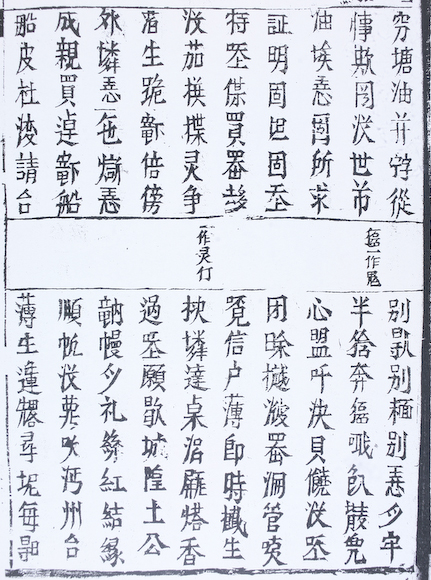
\includegraphics[scale=2.6,clip=true, trim=2.25cm 0 .125cm 0]{kieu1902/page107.jpg} }
\newpage
\hspace*{-1.75cm}\parbox{.65\textwidth}{
\item \bl{Một nhà dọn dẹp lanh chanh}{\một \nhà \dọn \dẹp \lanh \chanh}
\item \bl{Quét sân đặt trác rửa bình thắp hương}{\quét \sân \đặt \trác \rửa \bình \thắp \hương}
\item \bl{Bạc sinh quỳ xuống vội vàng}{\BẠC \sinh \quỳ \xuống \vộivàng}
\item \bl{Quá lời nguyện hết Thành hoàng Thổ công}{\quá \Lời   \nguyện \hết \thành \HOàng \thổ \công}
\item \bl{Ngoài sân lòng đã tỏ lòng}{\ngoài \sân \lòng \đã \TỎ\lòng}
\item \bl{Trong màn làm lễ tơ hồng kết duyên}{\trong \màn \làm \lễ \tơ \hồng \kết \duyên}
\item \bl{Thành thân mới rước xuống thuyền}{\thành \THân\mới \rước \xuống \thuyền}
\item \bl{Thuận buồm một lá xuôi miền Châu Thai}{\thuận \buồm \một \lá \xuôi \miền \Châu \thai}
\item \bl{Thuyền vừa đỗ bến thảnh thơi}{\thuyền \vừa \đỗ \bến \thảnhthơi}
\item \bl{Bạc sinh lên trước tìm nơi mọi ngày}{\BẠC \sinh \lên \trước \tìm \nơi \mọi \ngày}
}\parbox{.35\textwidth}{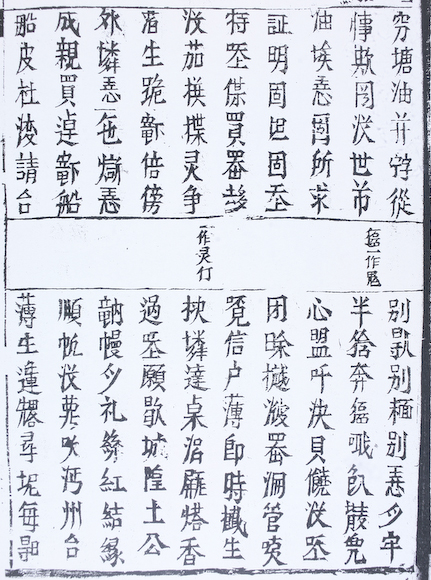
\includegraphics[scale=2.6,clip=true, trim=0cm 0 2.25cm 0]{kieu1902/page107.jpg} }
\newpage
\hspace*{-1.75cm}\parbox{.65\textwidth}{
\item \bl{Cũng nhà hành viện xưa nay}{\cũng \nhà \hành \viện \xưanay}
\item \bl{Cũng phường bán thịt cũng tay buôn người}{\cũng \phường \bán \Thịt \cũng \tay \buôn \người}
\item \bl{Xem người định giá vừa rồi}{\xem \người \định \giá \vừa \rồi}
\item \bl{Mối hàng một đã ra mười thì buôn}{\mối \Hàng \một \đã \ra \mười \thì \buôn}
\item \bl{Mượn người thuê kiệu rước nàng}{\mượn \người \thuê \kiệu \rước \nàng}
\item \bl{Bạc đem mặt bạc kiếm đường cho xa}{\Bạc \đem \mặt \Bạc \kiếm \đường \cho \xa}
\item \bl{Kiệu hoa đặt trước thềm hoa}{\kiệu \hoa \đặt \trước \thềm \hoa}
\item \bl{Bên trong thấy một mụ ra vội vàng}{\bên \trong \thấy \một \mụ \ra \vộivàng}
\item \bl{Đưa nàng vào lạy gia đường}{\đưa \nàng \vào \lạy \gia \Đường}
\item \bl{Cũng thần mày trắng cũng phường lầu xanh}{\cũng \thần \mày  \trắng \cũng \phường \lầu \xanh}
}\parbox{.35\textwidth}{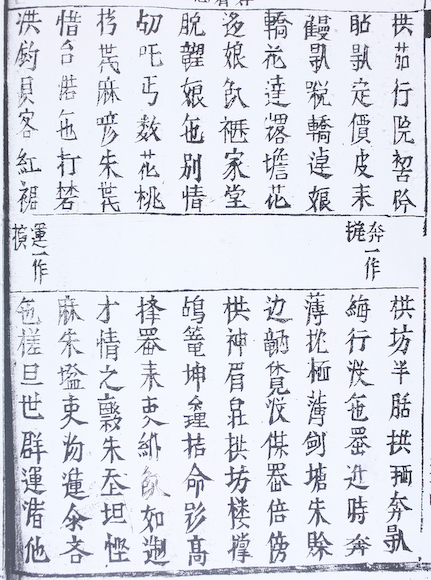
\includegraphics[scale=2.6,clip=true, trim=2.25cm 0 .125cm 0]{kieu1902/page108.jpg} }\newpage
\hspace*{-1.75cm}\parbox{.65\textwidth}{
\item \bl{Thoắt trông nàng đã biết tình}{\thoắt \trông \nàng \đã \biết \tình}
\item \bl{Chim lồng khôn nhẽ cất mình bay cao}{\chim \lồng \khôn \nhẽ \cất \mình \bay \Cao}
\item \bl{Chém cha cái số hoa đào}{\chém \cha \cái \số \hoa \đào}
\item \bl{Gỡ ra rồi lại buộc vào như chơi}{\gỡ \ra \rồi \lại \BUỘc \vào\như  \chơi}
\item \bl{Nghĩ đời mà ngán cho đời}{\nghĩ \đời \mà \ngán \cho \đời}
\item \bl{Tài tình chi lắm cho trời đất ghen}{\tài \tình \chi \lắm \cho \trời \đất \ghen}
\item \bl{Tiếc thay nước đã đánh phèn}{\tiếc \Thay \nước \đã \đánh \phèn}
\item \bl{Mà cho bùn lại vẩn lên mấy lần}{\mà \cho \bùn \lại \vẩn \lên \mấy \lần}
\item \bl{Hồng quân với khách hồng quần}{\Hồng \QUÂn \với \khách \hồng \quần}
\item \bl{Đã xoay đến thế còn vần chưa tha}{\đã \xoay \đến \thế  \Còn  \vần \chưa \tha}
}\parbox{.35\textwidth}{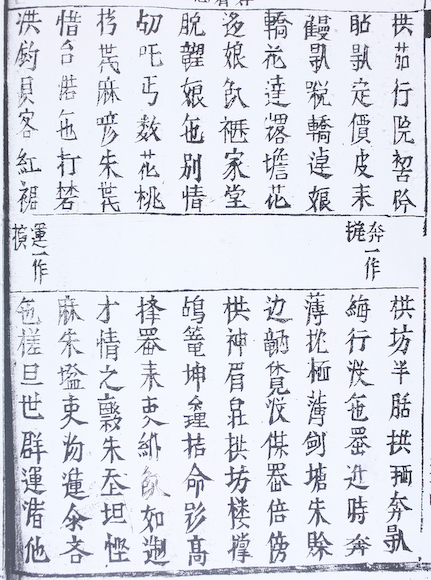
\includegraphics[scale=2.6,clip=true, trim=0.1cm 0 2.25cm 0]{kieu1902/page108.jpg} }\newpage
\hspace*{-1.75cm}\parbox{.65\textwidth}{
\item \bl{Lỡ từ lạc bước bước ra}{\lỡ \từ \lạc \bước \bước \ra}
\item \bl{Cái thân liệu những từ nhà liệu đi}{\cái \thân \liệu \những \từ \nhà \liệu \đi}
\item \bl{Đầu xanh đã tội tình gì}{\Đầu  \xanh \đã \tội \tình \gì}
\item \bl{Má hồng đền quá nửa thì chưa thôi}{\má \hồng \đền \quá \nửa \thì \chưa \thôi}
\item \bl{Biết thân chạy chẳng khỏi trời}{\biết \thân \Chạy  \chẳng \khỏi \trời}
\item \bl{Cũng liều mặt phấn cho rồi ngày xanh}{\cũng \liều \mặt \phấn \cho \rồi \ngày \xanh}
\item \bl{Lần lừa gió mát trăng thanh}{\lần \lừa \gió \mát \trăng \Thanh }
\item \bl{Bỗng đâu có khách biên đình sang chơi}{\bỗng \đâu \có \khách \biên\Đình \sang \chơi}
\item \bl{Râu hùm hàm én mày ngài}{\râu \hùm \hàm \én \mày  \ngài}
\item \bl{Vai năm tấc rộng thân mười thước cao}{\vai \Năm  \tấc \rộng \thân \mười \thước \Cao}
}\kieur{109}\newpage
\hspace*{-1.75cm}\parbox{.65\textwidth}{
\item \bl{Đường đường một đấng anh hào}{\đườngđường \một \đấng \anhhào}
\item \bl{Côn quyền hơn sức lược thao gồm tài}{\côn \quyền \hơn \sức \Lược \Thao \gồm \tài}
\item \bl{Đội trời đạp đất ở đời}{\đội \trời \đạp \đất \ở \đời}
\item \bl{Họ Từ tên Hải vốn người Việt Đông}{\họ \TỪ \tên \hải \vốn \người \việtđông}
\item \bl{Giang hồ quen thú vẫy vùng}{\gianghồ \quen \thú \vẫy \vùng}
\item \bl{Gươm đàn nửa gánh non sông một chèo}{\gươm \đàn \nửa \gánh \non \sông \một \chèo}
\item \bl{Qua chơi nghe tiếng nàng Kiều}{\qua \chơi \nghe \tiếng \nàng \kiều}
\item \bl{Tấm lòng nhi nữ dễ xiêu anh hùng}{\tấm \lòng \nhi \nữ \dễ \xiêu \anhhùng}
\item \bl{Thiếp danh đưa đến lầu hồng}{\Thiếp \danh \đưa \đến \lầu \hồng}
\item \bl{Hai bên cùng liếc hai lòng cùng ưa}{\hai \bên \Cùng \liếc \hai \lòng \Cùng \ưa}
}\kieull{109}\newpage
\hspace*{-1.75cm}\parbox{.65\textwidth}{
\item \bl{Từ rằng: Tâm phúc tương cờ}{\TỪ \rằng \tâm \Phúc \tương \CỜ}
\item \bl{Phải người trăng gió vật vờ hay sao}{\phải \người \trăng \gió \vậtvờ \hay \SAO }
\item \bl{Bấy lâu nghe tiếng má đào}{\Bấylâu \nghe \tiếng \má \đào}
\item \bl{Mắt xanh chẳng để ai vào có không}{\mắt \xanh \chẳng \để \ai \vào \có \không}
\item \bl{Một đời được mấy anh hùng}{\một \đời \được \mấy \anhhùng}
\item \bl{Bõ chi cá chậu chim lồng mà chơi}{\Bõ \chi \cá \chậu \chim \lồng \mà \chơi}
\item \bl{Nàng rằng: Người dạy quá lời}{\nàng \rằng \người \dạy \quá \Lời  }
\item \bl{Thân này còn dám xem ai làm thường}{\thân \này  \Còn  \dám \xem \ai \làm \thường}
\item \bl{Chút riêng chọn đá thử vàng}{\chút \riêng \chọn \Đá \thử \vàng}
\item \bl{Biết đâu mà gởi can trường vào đâu}{\biết \đâu \mà \gởi \cantrường \vào \đâu}
}\kieurr{110}\newpage
\hspace*{-1.75cm}\parbox{.65\textwidth}{
\item \bl{Còn như vào trước ra sau}{\Còn \như  \vào \trước \ra \sau}
\item \bl{Ai cho kén chọn vàng thau tại mình}{\ai \cho \kén \chọn \vàng \thau \tại \mình}
\item \bl{Từ rằng: Lời nói hữu tình}{\TỪ \rằng \Lời   \nói \hữu \tình}
\item \bl{Khiến người lại nhớ câu Bình Nguyên Quân}{\khiến \người \lại \nhớ \câu \bìnhnguyênquân}
\item \bl{Lại đây xem lại cho gần}{\lại \đây \xem \lại \cho \gần}
\item \bl{Phỏng tin được một vài phần hay không}{\phỏng \tin  \được \một \vài \phần \hay \không}
\item \bl{Thưa rằng: Lượng cả bao dong}{\thưa \rằng \lượng \cả \baodong }
\item \bl{Tấn Dương được thấy mây rồng có phen}{\tấndương \được \thấy \mây \rồng \có \phen}
\item \bl{Rộng thương cỏ nội hoa hèn}{\rộng \Thương \cỏ \nội \hoa \hèn}
\item \bl{Chút thân bèo bọt dám phiền mai sau}{\chút \thân \bèo \bọt \dám \phiền \maisau}
}\kieull{110}\newpage
\hspace*{-1.75cm}\parbox{.65\textwidth}{
\item \bl{Nghe lời vừa ý gật đầu}{\nghe \Lời   \vừa \ý \gật\Đầu }
\item \bl{Cười rằng: Tri kỷ thấy âu mấy người}{\cười \rằng \tri \kỷ \thấy \âu \mấy \người}
\item \bl{Khen cho con mắt tinh đời}{\khen \cho \con \mắt \tinh \đời}
\item \bl{Anh hùng biết giữa trần ai mới già}{\anhhùng \biết \Giữa \trần \ai \mới \già}
\item \bl{Một lời đã biết đến ta}{\một \Lời   \đã \biết \đến \ta}
\item \bl{Muôn chung nghìn tứ cũng là có nhau}{\muôn\Chung  \nghìn \tỨ \cũng \là  \có \nhau}
\item \bl{Hai bên ý hợp tâm đầu}{\hai \bên \ý \hợp \tâm\đầu}
\item \bl{Khi thân chẳng lọ là cầu mới thân}{\khi \THân\chẳng \lọ \là  \Cầu \mới \THân}
\item \bl{Sự lòng ngỏ với băng nhân}{\sự \lòng \ngỏ \với \băng \nhân}
\item \bl{Hai trăm lại cứ nguyên ngân chiếu hoàn}{\hai \trăm \lại \cứ \nguyên \ngân \chiếu \HOÀN}
}\kieur{111}\newpage
\hspace*{-1.75cm}\parbox{.65\textwidth}{
\item \bl{Buồng riêng sửa chốn thanh nhàn}{\buồng \riêng \sửa \chốn \thanhnhàn}
\item \bl{Đặt giường thất bảo vây màn bát tiên}{\Đặt \giường \thất \BẢo  \Vây \màn \bát \tiên}
\item \bl{Trai anh hùng gái thuyền quyên}{\Trai \anhhùng \gái \thuyềnquyên}
\item \bl{Phỉ nguyền bói phượng đẹp duyên cưỡi rồng}{\phỉ \nguyền \bói \phượng \ĐẸP \duyên \cưỡi \rồng}
\item \bl{Nửa năm hương lửa đương nồng}{\nửa \NĂM \hương \lửa \đương \nồng}
\item \bl{Trượng phu thoắt đã động lòng bốn phương}{\trượng \phu \thoắt \đã \động \lòng \bốn \phương}
\item \bl{Trông vời trời bể mênh mang}{\trông \vời \trời \bể \mênh \mang}
\item \bl{Thanh gươm yên ngựa lên đường thẳng giong}{\THanh \gươm \yênngựa \lên \đường \Thẳng \giong}
\item \bl{Nàng rằng: Phận gái chữ tòng}{\nàng \rằng \phận \gái \Chữ \tòng}
\item \bl{Chàng đi thiếp cũng một lòng xin đi}{\chàng \đi \thiếp \cũng \một \lòng \xin \đi}
}\kieul{111}\newpage
\hspace*{-1.75cm}\parbox{.65\textwidth}{
 \item \bl{Từ rằng: Tâm phủ tương tri}{\TỪ \rằng \tâm \PHỦ \tương \tri}
\item \bl{Sao chưa thoát khỏi nữ nhi thường tình}{\SAO  \chưa \thoát \khỏi \nữ \nhi \thường \tình}
\item \bl{Bao giờ mười vạn tinh binh}{\baogiờ \mười \vạn \tinh \binh}
\item \bl{Tiếng bề dậy đất bóng tinh rợp đường}{\tiếng \Bề \dậy \đất \bóng \Tinh \rợp \đường}
\item \bl{Làm cho rõ mặt phi thường}{\làm \cho \rõ \mặt \phithường}
\item \bl{Bấy giờ ta sẽ rước nàng nghi gia}{\bấy \giờ \ta \sẽ \rước \nàng \NGHi \gia}
\item \bl{Bằng nay bốn bể không nhà}{\bằng \nay \bốn \bể \không \nhà}
\item \bl{Theo càng thêm bận biết là đi đâu}{\theo \càng \thêm \bận \biết \là  \đi \đâu}
\item \bl{Đành lòng chờ đó ít lâu}{\đành \lòng \chờ \đó \ít \lâu}
\item \bl{Chầy chăng là một năm sau vội gì}{\chầy \chăng \là  \một \NĂM \sau \vội \gì}
}\kieurr{112}\newpage
\hspace*{-1.75cm}\parbox{.65\textwidth}{
\item \bl{Quyết lời dứt áo ra đi}{\quyết \Lời   \DỨt \áo \ra \đi}
\item \bl{Gió đưa bằng tiện đã lìa dặm khơi}{\gió \đưa \BẰng \tiện \đã \lìa \dặm \Khơi}
\item \bl{Nàng từ chiếc bóng song mai}{\nàng \từ \chiếc \bóng \SOng \mai}
\item \bl{Đêm thâu đằng đẵng nhặt cài then mây}{\đêm \thâu \đằng \đẵng \Nhặt \cài \then \mây}
\item \bl{Sân rêu chẳng vẽ dấu giày}{\sân \Rêu \chẳng \vẽ \dấu \giày }
\item \bl{Cỏ cao hơn thước liễu gầy vài phân}{\cỏ \Cao \hơn \thước \liễu \gầy \vài \phân}
\item \bl{Đoái trông muôn dặm tử phần}{\đoái \trông \muôn \dặm \tửphần}
\item \bl{Hồn quê theo ngọn mây Tần xa xa}{\hồn \quê \theo \ngọn \mây \tần \xa \xa}
\item \bl{Xót thay huyên cỗi xuân già}{\xót \Thay \Huyên \cỗi \Xuân \già }
\item \bl{Tấm lòng thương nhớ biết là có nguôi}{\tấm \lòng \Thương \nhớ \biết \là  \có \nguôi}
}\kieull{112}\newpage
\hspace*{-1.75cm}\parbox{.65\textwidth}{
\item \bl{Chốc là mười mấy năm trời}{\chốc \là \mười \mấy \NĂM \trời}
\item \bl{Còn ra khi đã da mồi tóc sương}{\Còn  \ra \khi \đã \damồi \tóc \sương}
\item \bl{Tiếc thay chút nghĩa cũ càng}{\tiếc \Thay \chút \Nghĩa \cũ \càng}
\item \bl{Dẫu lìa ngó ý còn vương tơ lòng}{\dẫu \lìa \ngó \ý \Còn  \vương \tơ \lòng}
\item \bl{Duyên em dầu nối chỉ hồng}{\duyên \em \dầu \nối\CHỈ \hồng}
\item \bl{Lẽ ra khi đã tay bồng tay mang}{\lẽ \ra \khi \đã \tay \Bồng \tay \mang}
\item \bl{Tấc lòng cố quốc tha hương}{\tấc \lòng \cố \quốc \thahương}
\item \bl{Đường kia nỗi nọ ngổn ngang bời bời}{\đường \kia \nỗi \nọ \ngổnngang \bời \bời}
\item \bl{Cánh hồng bay bổng tuyệt vời}{\cánh \HỒng \bay \bổng \tuyệt \vời}
\item \bl{Đã mòn con mắt phương trời đăm đăm}{\đã \mòn \con \mắt \phương \trời \đăm \đăm}
}\kieur{113}\newpage
\hspace*{-1.75cm}\parbox{.65\textwidth}{
\item \bl{Đêm ngày luống những âm thầm}{\Đêm \ngày \luống \những \âmthầm}
\item \bl{Lửa binh đâu đã ầm ầm một phương}{\lửa \binh \đâu \đã \ầm \ầm \một \phương}
\item \bl{Ngất trời sát khí mơ màng}{\ngất \trời \Sát \khí \mơ \màng}
\item \bl{Đầy sông kình ngạc chật đường giáp binh}{\đầy \sông \kình \ngạc \chật \đường \GIáp  \binh}
\item \bl{Người quen thuộc, kẻ chung quanh}{\người \quen \thuộc \kẻ \chung \quanh}
\item \bl{Nhủ nàng hãy tạm lánh mình một nơi}{\nhủ \nàng \hãy \tạm \lánh \mình \một \nơi}
\item \bl{Nàng rằng: Trước đã hẹn lời}{\nàng \rằng \trước \đã \hẹn \Lời  }
\item \bl{Dẫu trong nguy hiểm dám rời ước xưa}{\dẫu \trong \nguy \hiểm \Dám \rời \ước \xưa}
\item \bl{Còn đang dùng dắng ngẩn ngơ}{\Còn  \đang \dùng \dắng \Ngẩnngơ}
\item \bl{Mái ngoài đã thấy bóng cờ tiếng la}{\mái \ngoài \đã \thấy \bóng \cờ \tiếngla}
}\kieul{113}\newpage
\hspace*{-1.75cm}\parbox{.65\textwidth}{
\item \bl{Giáp binh kéo đến quanh nhà}{\GIáp  \binh \kéo \đến \quanh \nhà}
\item \bl{Đồng thanh cùng gởi nào là phu nhân}{\Đồng \thanh \Cùng \gởi \nào  \là  \phu \nhân}
\item \bl{Hai bên mười vị tướng quân}{\hai \bên \mười \vị \tướng\Quân }
\item \bl{Đặt gươm cởi giáp trước sân khấu đầu}{\Đặt \gươm \cởi \GIáp  \trước \sân \khấu\Đầu }
\item \bl{Cung nga thể nữ theo sau}{\cung \nga \thểnữ \theo \sau}
\item \bl{Rằng: Vâng lệnh chỉ rước chầu vu quy}{\rằng \vâng \lệnh \Chỉ \rước \chầu \vu \quy}
\item \bl{Sẵn sàng phượng liễn loan nghi}{\sẵn \sàng \phượng \liễn \loan \Nghi}
\item \bl{Hoa quan giấp giới hà y rỡ ràng}{\hoaquan \giấpgiới \Hà \y \rỡràng}
\item \bl{Dựng cờ nổi trống lên đường}{\dựng \cờ \nổi \trống \lên \đường}
\item \bl{Trúc tơ dậy trước kiệu vàng kéo sau}{\trúc \tơ \Dậy \trước \kiệu \vàng \kéo \sau}
}\kieur{114}\newpage
\hspace*{-1.75cm}\parbox{.65\textwidth}{
\item \bl{Hỏa bài tiền lộ ruổi mau}{\hỏa \Bài  \Tiền \lộ \ruổi \Mau}
\item \bl{Nam đình nghe động trống chầu đại doanh}{\nam\Đình \nghe \động \Trống \chầu \đại \Doanh}
\item \bl{Kéo cờ lũy phát súng thành}{\kéo \cờ \lũy  \phát \súng \thành}
\item \bl{Từ công ra ngựa thân nghênh cửa ngoài}{\TỪ \công \ra \ngựa \THân\nghênh \cửa \ngoài}
\item \bl{Rỡ mình là vẻ cân đai}{\Rỡ \mình \là  \vẻ \cân \đai}
\item \bl{Hãy còn hàm én mày ngài như xưa}{\hãy \Còn  \hàm \én \mày  \NGài\như  \xưa}
\item \bl{Cười rằng: Cá nước duyên ưa}{\cười \rằng \cá \nước \duyên \ưa}
\item \bl{Nhớ lời nói những bao giờ hay không}{\nhớ \Lời   \nói \những \baogiờ \hay \không}
\item \bl{Anh hùng mới biết anh hùng}{\anhhùng \mới \biết \anhhùng}
\item \bl{Rày xem phỏng đã cam lòng ấy chưa}{\rày \xem \phỏng \đã \cam \lòng \ấy \Chưa}
}\kieull{114}\newpage
\hspace*{-1.75cm}\parbox{.65\textwidth}{
\item \bl{Nàng rằng: Chút phận ngây thơ}{\nàng \rằng \chút \phận \ngâythơ}
\item \bl{Cũng may dây cát được nhờ bóng cây}{\cũng \may \dây \CÁt \được \nhờ \bóng \cây}
\item \bl{Đến bây giờ mới thấy đây}{\đến \bâygiờ \mới \thấy \đây}
\item \bl{Mà lòng đã chắc những ngày một hai}{\mà \lòng \đã \chắc \những \ngày \một \hai}
\item \bl{Cùng nhau trông mặt cả cười}{\Cùng \nhau \trông \mặt \cả \cười}
\item \bl{Dan tay về chốn trướng mai tự tình}{\Dan \tay \về \chốn \trướng \mai \tựtình}
\item \bl{Tiệc bày thưởng tướng khao binh}{\tiệc \bày \thưởng \tướng \Khao \binh}
\item \bl{Ầm thùng trống trận rập rình nhạc quân}{\ầmthùng \Trống \trận \rập \rình \Nhạc\Quân }
\item \bl{Vinh hoa bõ lúc phong trần}{\vinh \hoa \bõ \lúc \phongtrần}
\item \bl{Chữ tình ngày một thêm xuân một ngày}{\Chữ \tình \ngày \một \thêm \xuân \một \ngày}
}\kieur{115}\newpage
\hspace*{-1.75cm}\parbox{.65\textwidth}{
\item \bl{Trung quân nhân lúc vui vầy}{\trung \Quân\NHân \lúc \vuivầy}
\item \bl{Thong dong mới kể chuyện ngày hàn vi}{\thongdong \mới \kể \chuyện \ngày \hànvi}
\item \bl{Khi Vô tích khi Lâm tri}{\khi \vôtích \khi \lâmtri}
\item \bl{Nơi thì lừa đảo nơi thì xót thương}{\nơi \thì \lừa \đảo \nơi \thì \xót \Thương }
\item \bl{Tấm thân rày đã nhẹ nhàng}{\tấm \thân \rày \đã \nhẹ \nhàng}
\item \bl{Chút còn ân oán đôi đường chưa xong}{\chút \Còn  \ân \oán \đôi \đường \chưa \xong}
\item \bl{Từ công nghe nói thủy chung}{\TỪ \công \nghe \nói \thủychung}
\item \bl{Bất bình nổi trận đùng đùng sấm vang}{\bấtbình \nổi \trận \đùng \đùng \sấm \vang}
\item \bl{Nghiêm quân chọn tướng sẵn sàng}{\nghiêm\Quân \Chọn \tướng \sẵn \sàng}
\item \bl{Dưới cờ một lệnh vội vàng ruổi sao}{\dưới \cờ \một \lệnh \vộivàng \ruổi \Sao }
}\kieul{115}\newpage
\hspace*{-1.75cm}\parbox{.65\textwidth}{
\item \bl{Ba quân chỉ ngọn cờ đào}{\ba\Quân \CHỉ \ngọn \cờ \đào}
\item \bl{Đạo ra Vô tích đạo vào Lâm tri}{\đạo \ra \vôtích \đạo \vào \lâmtri}
\item \bl{Mấy người phụ bạc xưa kia}{\mấy \người \phụbạc \xưa \kia}
\item \bl{Chiếu danh truy nã đem về hỏi tra}{\chiếu \danh \truy \nã \đem \về \hỏi \tra}
\item \bl{Lại sai lệnh tiễn truyền ra}{\lại \sai \lệnh \tiễn \truyền \ra}
\item \bl{Giữ gìn họ Thúc một nhà cho yên}{\giữ  \gìn \họ \thúc \một \nhà \cho \yên}
\item \bl{Mụ quản gia, vãi Giác Duyên}{\mụ \quản \gia \vãi \giácduyên}
\item \bl{Cũng sai lệnh tiễn đem tin rước mời}{\cũng \sai \lệnh \tiễn \đem \tin  \rước \mời}
\item \bl{Thệ sư kể hết mọi lời}{\thệ \sư \kể \hết \mọi \Lời  }
\item \bl{Lòng lòng cũng giận người người chấp uy}{\lòng \lòng \Cũng \giận \người \người \chấp \uy}
}\kieurr{116}\newpage
\hspace*{-1.75cm}\parbox{.65\textwidth}{
\item \bl{Đạo trời báo phục chỉn ghê}{\đạo \trời \báo \Phục \Chỉn \ghê}
\item \bl{Chia đi mọi ngả tóm về đòi nơi}{\Chia \đi \mọi \ngả \tóm \về \đòi \nơi}
\item \bl{Quân trung gươm lớn giáo dài}{\Quân\trung \gươm \lớn \giáo \dài}
\item \bl{Vệ trong thị lập cơ ngoài song phi}{\Vệ \trong \thị \Lập \cơ \ngoài \song  \phi}
\item \bl{Sẵn sàng tề chỉnh uy nghi}{\sẵnsàng \tềchỉnh \uynghi}
\item \bl{Bác đồng chật đất tinh kỳ rợp sân}{\bác  \ĐỒng \chật \đất \tinhkỳ \rợp \sân}
\item \bl{Trướng hùm mở giữa trung quân}{\trướng \hùm \mở \Giữa \trung\Quân }
\item \bl{Từ công sánh với phu nhân cùng ngồi}{\TỪ \công \sánh \với \phu \nhân \Cùng \ngồi}
\item \bl{Tiên nghiêm trống chửa dứt hồi}{\Tiên \nghiêm \trống \chửa \dứt \hồi}
\item \bl{Điểm danh trước dẫn chực ngoài cửa viên}{\điểm \danh \trước \dẫn \chực \ngoài \cửa \VIên}
}\kieull{116}\newpage
\hspace*{-1.75cm}\parbox{.65\textwidth}{
\item \bl{Từ rằng: Ân oán đôi bên}{\TỪ \rằng \ân \oán \đôi \bên}
\item \bl{Mặc nàng xử quyết báo đền cho minh}{\mặc \nàng \xử \quyết \báo \đền \cho \minh}
\item \bl{Nàng rằng: Muôn cậy oai linh}{\nàng \rằng \muôn \cậy \oai \linh}
\item \bl{Hãy xin báo đáp ân tình cho phu}{\hãy \xin \báo \đáp \ân \tình \cho \Phu}
\item \bl{Báo ân rồi sẽ trả thù}{\báo \ân \rồi \sẽ \trả \thù}
\item \bl{Từ rằng: Việc ấy để cho mặc nàng}{\TỪ \rằng \việc \ấy \để \cho \mặc \nàng}
\item \bl{Sổ tên trước xướng Thúc lang}{\sổ \tên \trước \xướng \thúclang}
\item \bl{Mặt như chàm đổ mình dường giẽ run}{\mặt\như  \chàm \Đổ \mình \dường \giẽ \run}		
\item \bl{Nàng rằng: Nghĩa nặng nghìn non}{\nàng \rằng \Nghĩa  \nặng \nghìn \non}
\item \bl{Lâm Tri  người cũ chàng còn nhớ không}{\lâmtri \người \cũ \chàng \Còn  \nhớ \không}
}\kieurr{117}\newpage
\hspace*{-1.75cm}\parbox{.65\textwidth}{
\item \bl{Sâm Thương chẳng vẹn chữ tòng}{\sâm \thương\chẳng \vẹn \Chữ \tòng}
\item \bl{Tại ai há dám phụ lòng cố nhân}{\tại \ai \há \Dám \Phụ \lòng \cố \nhân}
\item \bl{Gấm trăm cuốn bạc nghìn cân}{\gấm \trăm \Cuốn \BẠC \nghìn \cân}
\item \bl{Tạ lòng dễ xứng báo ân gọi là}{\tạ \lòng \dễ \Xứng \báo \ân \gọi \là}
\item \bl{Vợ chàng quỷ quái tinh ma}{\vợ \chàng \quỷ \quái \tinh \ma}
\item \bl{Phen này kẻ cắp bà già gặp nhau}{\phen \này  \kẻ \cắp \Bà \già\gặp \nhau}
\item \bl{Kiến bò miệng chén chưa lâu}{\Kiến \bò \Miệng \chén \chưa \lâu}
\item \bl{Mưu sâu đành trả nghĩa sâu cho vừa}{\mưu \sâu \Đành \trả \Nghĩa  \sâu \cho \vừa}
\item \bl{Thúc sinh trông mặt bấy giờ}{\thúc\sinh \trông \mặt \bấygiờ}
\item \bl{Mồ hôi chàng đã như mưa ướt đầm}{\Mồ \hôi \chàng \đã\như  \mưa \ướt \đầm}
}\kieull{117}\newpage
\hspace*{-1.75cm}\parbox{.65\textwidth}{
 \item \bl{Lòng riêng mừng sợ khôn cầm}{\lòng \riêng \mừng \sợ \khôn \cầm}
\item \bl{Sợ thay mà lại mừng thầm cho ai}{\sợ \thay \mà \lại \mừng \thầm \cho \ai}
\item \bl{Mụ già, sư trưởng thứ hai}{\mụ \già\sư \trưởng \thứ \hai}
\item \bl{Thoắt đưa đến trước vội mời lên trên}{\thoắt \đưa \đến \trước \vội \mời \lên \trên}
\item \bl{Dắt tay mở mặt cho nhìn}{\dắttay \mở \mặt \cho \nhìn}
\item \bl{Hoa nô kia với Trạc Tuyền cũng tôi}{\hoa \nô \kia \với \trạctuyền \cũng \tôi}
\item \bl{Nhớ khi lỡ bước sẩy vời}{\nhớ \khi \LỠ \bước \sẩy \vời}
\item \bl{Non vàng chưa dễ đền bồi tấm thương}{\non \vàng \chưa \dễ \đền \Bồi \tấm \Thương }
\item \bl{Nghìn vàng gọi chút lễ thường}{\nghìn \vàng \gọi \chút \lễ \thường}
\item \bl{Mà lòng Phiếu mẫu mấy vàng cho cân}{\mà \lòng \phiếu \mẫu \mấy \vàng \cho \cân}
}\kieurr{118}\newpage
\hspace*{-1.75cm}\parbox{.65\textwidth}{
\item \bl{Hai người trông mặt tần ngần}{\hai \người \trông \mặt \tần \ngần}
\item \bl{Nửa phần khiếp sợ nửa phần mừng vui}{\nửa \phần \khiếp \sợ \nửa \phần \mừng \vui}
\item \bl{Nàng rằng: Xin hãy rốn ngồi}{\nàng \rằng \xin \hãy \rốn \ngồi}
\item \bl{Xem cho rõ mặt biết tôi báo thù}{\xem \cho \rõ \mặt \biết \tôi \báothù}
\item \bl{Kíp truyền chư tướng hiến phù}{\kíp  \truyền \chư \tướng \hiếnphù}
\item \bl{Lại đem các tích phạm tù hậu tra}{\lại \đem \Các \Tích \phạm \tù \hậu \tra}
\item \bl{Dưới cờ gươm tuốt hộp ra}{\dưới \cờ \gươm \tuốt \hộp \ra}
\item \bl{Chính danh thủ phạm tên là Hoạn Thư}{\chính \danh \thủ \phạm \tên \là  \hoạnthư}
\item \bl{Xa trông nàng đã chào thưa}{\xa \trông \nàng \đã \chào \thưa}
\item \bl{Tiểu thư cũng có bi giờ đến đây}{\tiểuthư \cũng \có \bigiờ \đến \đây}
}\kieul{118}\newpage
\hspace*{-1.75cm}\parbox{.65\textwidth}{
\item \bl{Đàn bà dễ có mấy tay}{\đànbà \dễ \có \mấy \tay}
\item \bl{Đời xưa mấy mặt đời này mấy gan}{\đời \xưa \mấy \mặt \đời \này  \mấy \gan}
\item \bl{Dễ dàng là thói hồng nhan}{\dễ \dàng \là  \thói \hồng \nhan}
\item \bl{Càng gây nghiệt lắm càng oan trái nhiều}{\càng \gây \nghiệt \lắm \càng \Oan \trái \nhiều}
\item \bl{Hoạn thư  phách lạc  hồn xiêu}{\hoạnthư  \phách\lạc  \hồn \xiêu}
\item \bl{Khấu đầu dưới trướng lựa điều kêu ca}{\khấu\Đầu  \dưới \trướng \lựa \Điều  \kêu \Ca}%\hspace*{-.15cm}\CA}
\item \bl{Rằng: Tôi chút dạ đàn bà}{\rằng \tôi \chút \Dạ \đànbà}
\item \bl{Ghen tuông thì cũng người ta thường tình}{\ghen \tuông \thì \cũng \người \ta \thường \tình}
\item \bl{Nghĩ cho khi các viết kinh}{\nghĩ \cho \khi \các \viết \Kinh}
\item \bl{Với khi khỏi cửa dứt tình chẳng theo}{\với \khi \khỏi \cửa \dứt \tình \chẳng \theo}
}\kieur{119}\newpage
\hspace*{-1.75cm}\parbox{.65\textwidth}{
\item \bl{Lòng riêng riêng những kính yêu}{\lòng \riêng \riêng \những \kính \Yêu}
\item \bl{Chồng chung chưa dễ ai chiều cho ai}{\chồng \chung \chưa \dễ \ai \chiều \cho \ai}
\item \bl{Trót đà gây việc chông gai}{\Trót  \đà \gây \Việc \chông \gai}
\item \bl{Còn nhờ lượng bể thương bài cho chăng}{\Còn  \nhờ \lượng \bể \Thương \bài \cho \chăng}
\item \bl{Khen cho khéo đã nên rằng}{\khen \cho \khéo \đã \nên \rằng}
\item \bl{Khôn ngoan đến mực nói năng phải lời}{\khôn \ngoan \đến \mực \nói \năng \phải \Lời  }
\item \bl{Tha ra thì cũng may đời}{\tha \ra \thì \cũng \may \đời}
\item \bl{Làm ra thì cũng ra người nhỏ nhen}{\làm \ra \thì \cũng \ra \người \nhỏ \nhen}
\item \bl{Đã lòng tri quá thì nên}{\đã \lòng \tri \quá \thì \nên}
\item \bl{Truyền quân lệnh xuống trướng tiền tha ngay}{\truyền\Quân \lệnh \xuống \trướng \Tiền \tha \Ngay }
}\kieul{119}\newpage


\hspace*{-1.75cm}\parbox{.65\textwidth}{
\item \bl{Tạ lòng lạy trước sân mây}{\tạ \lòng \lạy \trước \sân \mây}
\item \bl{Cửa hiên lại dắt một dây dẫn vào}{\cửa  \hiên\lại \Dắt \một \dây \dẫn \vào}
\item \bl{Nàng rằng: Lồng lộng trời cao}{\nàng \rằng \lồng \lộng \trời \Cao}
\item \bl{Hại nhân nhân hại sự nào tại ta}{\hại \nhân \nhân \hại \sự \nào  \tại \ta}
\item \bl{Nào là Bạc Hạnh Bạc bà}{\nàolà \BẠC \hạnh \BẠC \bà}
\item \bl{Nào là Ưng Khuyển nào là Sở Khanh}{\nàolà \ưng \khuyển \nàolà \sởkhanh}
\item \bl{Tú bà với Mã Giám sinh}{\tú \Bà \với \mã \giám \sinh}
\item \bl{Các tên tội ấy đáng tình còn sao}{\Các \tên \tội \ấy \đáng \tình \Còn  \SAO }
\item \bl{Lệnh quân truyền xuống khai đao}{\lệnh\Quân \truyền \xuống \khai \đao}
\item \bl{Thề sao thì lại cứ sao gia hình}{\thề \SAO  \thì \lại \cứ \SAO  \GIa \hình}
}\kieurr{120}\newpage
\hspace*{-1.75cm}\parbox{.65\textwidth}{
\item \bl{Máu rơi thịt nát tan tành}{\máu \rơi \thịt \Nát \tan \tành}
\item \bl{Ai ai trông thấy hồn kinh phách rời}{\ai \ai \trông \thấy \hồn \KINh \phách \rời}
\item \bl{Cho hay muôn sự tại trời}{\cho \hay \muôn \sự \tại \trời}
\item \bl{Phụ người chẳng bõ khi người phụ ta}{\Phụ \người \chẳng \Bõ \khi \người \Phụ \ta}
\item \bl{Mấy người bạc ác tinh ma}{\mấy \người \bạc \ác \tinh \ma}
\item \bl{Mình làm mình chịu kêu mà ai thương}{\mình \làm \mình \chịu \kêu \mà \ai \Thương }
\item \bl{Ba quân đông mặt pháp trường}{\ba\Quân  \Đông \mặt \pháp \trường}
\item \bl{Thanh thiên bạch nhật rõ ràng cho coi}{\THanh \THIên \bạch \nhật \rõ \ràng \cho \coi}
\item \bl{Việc nàng báo phục vừa rồi}{\Việc \nàng \báo \Phục \vừa \rồi}
\item \bl{Giác Duyên vội đã gởi lời từ quy}{\giácduyên \vội \đã \gởi \Lời  \Từ  \quy}
}\kieull{120}\newpage
\hspace*{-1.75cm}\parbox{.65\textwidth}{
\item \bl{Nàng rằng: Thiên tải nhất thì}{\nàng \rằng \THiên \tải \nhất \thì}
\item \bl{Cố nhân đã dễ mấy khi bàn hoàn}{\cố \nhân \đã \dễ \mấy \khi \Bànhoàn}
\item \bl{Rồi đây bèo hợp mây tan}{\rồi \đây \bèo \hợp \mây \tan}
\item \bl{Biết đâu hạc nội mây ngàn là đâu}{\biết \đâu \hạc \nội \mây \Ngàn \là  \đâu}
\item \bl{Sư rằng: Cũng chẳng bao lâu}{\sư \rằng \cũng \chẳng \bao \lâu}
\item \bl{Trong năm năm lại gặp nhau đó mà}{\trong \Năm\NĂM   \lại \gặp \nhau \đó \mà}
\item \bl{Nhớ ngày hành cước phương xa}{\nhớ \ngày \hành \cước \phương \xa}
\item \bl{Gặp sư Tam Hợp vốn là tiên tri}{\gặp \sư \tam \hợp \vốn \là  \tiêntri}
\item \bl{Bảo cho hội ngộ chi kỳ}{\Bảo \cho \hội \ngộ \chi \KỲ}
\item \bl{Năm nay là một nữa thì năm năm}{\năm \NAY \là  \một \nữa \thì \Năm\NĂM }
}\kieur{121}\newpage
\hspace*{-1.75cm}\parbox{.65\textwidth}{
\item \bl{Mới hay tiền định chẳng lầm}{\mới \hay \Tiền \định \chẳng \lầm}
\item \bl{Đã tin điều trước ắt nhằm việc sau}{\đã \tin  \Điều  \trước \ắt \nhằm \Việc \sau}
\item \bl{Còn nhiều ân nghĩa với nhau}{\Còn  \nhiều \ân \Nghĩa  \với \nhau}
\item \bl{Cơ duyên nào đã hết đâu vội gì}{\Cơ  \duyên \nào  \đã \hết \đâu \vội \gì}
\item \bl{Nàng rằng: Tiền định tiên tri}{\nàng \rằng \Tiền \định \Tiên \tri}
\item \bl{Lời sư đã dạy ắt thì chẳng sai}{\Lời   \sư \đã \dạy \ắt \thì \chẳng \sai}
\item \bl{Họa bao giờ có gặp người}{\HOạ  \baogiờ \có \gặp \người}
\item \bl{Vì tôi cậy hỏi một lời chung thân}{\Vì  \tôi \cậy \hỏi \một \Lời   \chung \thân}
\item \bl{Giác Duyên vâng dặn ân cần}{\giácduyên \vâng \dặn \âncần}
\item \bl{Tạ từ thoắt đã dời chân cõi ngoài}{\tạtừ \thoắt \đã \dời \chân \cõi \ngoài}
}\kieul{121}\newpage
\hspace*{-1.75cm}\parbox{.65\textwidth}{
\item \bl{Nàng từ ân oán rạch ròi}{\nàng \từ \ân \oán \Rạchròi}
\item \bl{Bể oan dường đã vơi vơi cạn lòng}{\bể \Oan \dường \đã \vơi \vơi \cạn \lòng}
\item \bl{Tạ ân lạy trước Từ công}{\tạ \ân \lạy \trước \TỪ \công}
\item \bl{Chút thân bồ liễu nào mong có rày}{\chút \thân \bồ \liễu \nào  \mong \có \rày}
\item \bl{Trộm nhờ sấm sét ra tay}{\trộm \nhờ \sấm \sét \ra \tay}
\item \bl{Tấc riêng như cất gánh đầy đổ đi}{\tấc \riêng\như  \cất \gánh \đầy \đổ \đi}
\item \bl{Chạm xương chép dạ xiết chi}{\chạm \xương \chép \Dạ \Xiết \chi}
\item \bl{Dễ đem gan óc đền nghì trời mây}{\dễ \đem \gan \óc \đền \nghì \trời \mây}
\item \bl{Từ rằng: Quốc sĩ xưa nay}{\TỪ \rằng \quốc \sĩ \xưanay}
\item \bl{Chọn người tri kỷ một ngày được chăng}{\chọn \người \tri \kỷ \một \ngày \được \chăng}
}\kieurr{122}\newpage
\hspace*{-1.75cm}\parbox{.65\textwidth}{
\item \bl{Anh hùng tiếng đã gọi rằng}{\anhhùng \tiếng \đã \gọi \rằng}
\item \bl{Giữa đường khi thấy bất bằng mà tha}{\Giữa \đường \khi \thấy \bất \Bằng \mà \tha}
\item \bl{Huống chi việc cũng việc nhà}{\huống \chi \việc \cũng \việc \nhà}
\item \bl{Lọ là thâm tạ mới là tri ân}{\lọ \là  \thâm \tạ \mới \là  \tri \ân}
\item \bl{Xót nàng còn chút song thân}{\xót \nàng \Còn  \chút \songthân}
\item \bl{Bấy lâu kẻ Việt người Tần cách xa}{\bấylâu \kẻ \việt \người \tần \cách \xa}
\item \bl{Sao cho muôn dặm một nhà}{\SAO  \cho \muôn \dặm \một \nhà}
\item \bl{Cho người thấy mặt là ta cam lòng}{\cho \người \thấy \mặt \là  \ta \cam \lòng}
\item \bl{Vội truyền sửa tiệc quân trung}{\vội \truyền \sửa \tiệc\Quân \trung}
\item \bl{Muôn binh nghìn tướng hội đồng tẩy oan}{\muôn \binh \nghìn \tướng \hội  \Đồng \tẩy \Oan}
}\kieull{122}\newpage
\hspace*{-1.75cm}\parbox{.65\textwidth}{
\item \bl{Thừa cơ trúc chẻ ngói tan}{\thừa \Cơ  \trúc \chẻ \ngói \tan}
\item \bl{Binh uy từ đó sấm ran trong ngoài}{\binh \uy \từ \đó \sấm \ran \trong \ngoài}
\item \bl{Triều đình riêng một góc trời}{\triều \ĐÌnh \riêng \một \góc \trời}
\item \bl{Gồm hai văn võ rạch đôi sơn hà}{\gồm \hai \văn \võ \rạch \đôi \sơn \hà}
\item \bl{Đòi cơn gió quét mưa sa}{\đòi \cơn \gió \quét \mưa \sa}
\item \bl{Huyện thành đạp đổ năm tòa hải nam}{\huyện \thành \đạp \đổ\ \Năm  \tòa \hải \nam}
\item \bl{Phong trần mài một lưỡi gươm}{\phongtrần \Mài \một \lưỡi \gươm}
\item \bl{Những loài giá áo túi cơm sá gì}{\những \loài \Giá  \áo \túi \cơm \Sá \gì}
\item \bl{Nghênh ngang một cõi biên thùy}{\nghênh \ngang \một \cõi \biênthùy}
\item \bl{Thiếu gì cô quả thiếu gì bá vương}{\thiếu \gì \Cô \quả \thiếu \gì \bá \vương}
}\kieurr{123}\newpage
\hspace*{-1.75cm}\parbox{.65\textwidth}{
\item \bl{Trước cờ ai dám tranh cường}{\trước \cờ \ai \Dám \Tranh \cường}
\item \bl{Năm năm hùng cứ một phương hải tần}{\Năm\NĂM \hùng \cứ \một \phương \hải \Tần}
\item \bl{Có quan tổng đốc trọng thần}{\có \quan \tổngđốc \trọng \Thần}
\item \bl{Là Hồ Tôn Hiến kinh luân gồm tài}{\là \hồtônhiến \Kinh \Luân \gồm \tài}
\item \bl{Đẩy xe vâng chỉ đặc sai}{\đẩy \xe \vâng \Chỉ \đặc \sai}
\item \bl{Tiện nghi phủ tiễu việc ngoài đổng nhung}{\tiện \NGHi \PHủ \tiễu \việc \ngoài \đổng \nhung}
\item \bl{Biết Từ là đấng anh hùng}{\biết \TỪ \là  \đấng \anhhùng}
\item \bl{Biết nàng cũng dự quân trung luận bàn}{\biết \nàng \cũng \dự\Quân \trung \luận \bàn}
\item \bl{Đóng quân làm chước chiêu an}{\đóng\Quân \làm \chước \chiêuan}
\item \bl{Phong thư mâm lễ sai quan thuyết hàng}{\PHONg \thư \mâm \lễ \sai \quan \thuyết \HÀng}
}\kieul{123}\newpage
\hspace*{-1.75cm}\parbox{.65\textwidth}{
\item \bl{Lại riêng một lễ với nàng}{\lại \riêng \một \lễ \với \nàng}
\item \bl{Hai tên thể nữ ngọc vàng nghìn cân}{\hai \tên \thểnữ \ngọc \vàng \nghìn \cân}
\item \bl{Tin vào gởi trước trung quân}{\tin  \vào \gởi \trước \trung\Quân }
\item \bl{Từ công riêng hãy mười phân hồ đồ}{\TỪ \công \riêng \hãy \mười \phân \hồđồ}
\item \bl{Một tay gây dựng cơ đồ}{\một \tay \gây \dựng \cơđồ}
\item \bl{Bấy lâu bể Sở sông Ngô tung hoành}{\bấy \lâu \bể \Sở \sông \ngô \tung \hoành}
\item \bl{Bó thân về với triều đình}{\bó \thân \về \với \triềuđình}
\item \bl{Hàng thần lơ láo phận mình ra đâu}{\HÀng \Thần \lơ \láo \phận \mình \ra \đâu}
\item \bl{Áo xiêm ràng buộc lấy nhau}{\áoxiêm \ràngbuộc \lấy \nhau}
\item \bl{Vào luồn ra cúi công hầu mà chi}{\vào \luồn \ra \cúi \công \hầu \mà \chi}
}\kieurr{124}\newpage
\hspace*{-1.75cm}\parbox{.65\textwidth}{
\item \bl{Sao bằng riêng một biên thùy}{\SAO  \bằng \riêng \một \biênthùy}
\item \bl{Sức này đã dễ làm gì được nhau}{\sức \này  \đã \dễ \làm \gì \được \nhau}
\item \bl{Chọc trời quấy nước mặc dầu}{\chọc \trời \quấy \nước \mặc \dầu}
\item \bl{Dọc ngang nào biết trên đầu có ai}{\dọcngang \nào  \biết \trên\Đầu  \có \ai}
\item \bl{Nàng thì thiệt dạ tin người}{\nàng \thì \thiệt \Dạ \tin  \người}
\item \bl{Của nhiều nói ngọt nghe lời dễ xiêu}{\của \nhiều \nói \ngọt \nghe \Lời   \dễ \xiêu}
\item \bl{Nghĩ mình mặt nước cánh bèo}{\nghĩ \mình \mặt \nước \cánh \bèo}
\item \bl{Đã nhiều lưu lạc lại nhiều gian truân}{\đã \nhiều \lưu \lạc \lại \nhiều \giantruân}
\item \bl{Bằng nay chịu tiếng vương thần}{\bằng \NAY \chịu \tiếng \vương \Thần}
\item \bl{Thênh thênh đường cái thanh vân hẹp gì}{\thênh \thênh \đường \cái \THanh \vân \hẹp \gì}
}\kieull{124}\newpage
\hspace*{-1.75cm}\parbox{.65\textwidth}{
\item \bl{Công tư vẹn cả hai bề}{\công \TƯ \vẹn \cả \hai \bề}
\item \bl{Dần dà rồi sẽ liệu về cố hương}{\dần \dà \rồi \sẽ \liệu \về \cố \Hương}
\item \bl{Cũng ngôi mệnh phụ đường đường}{\cũng \ngôi \mệnh \PHỤ \đườngđường}
\item \bl{Nở nang mày mặt rỡ ràng mẹ cha}{\nở \nang \mày  \mặt \rỡràng \mẹ \cha}
\item \bl{Trên vì nước dưới vì nhà}{\trên \Vì  \nước \dưới \Vì  \nhà}
\item \bl{Một là đắc hiếu hai là đắc trung}{\một \là \đắc \Hiếu \hai \là \đắc \Trung}
\item \bl{Chẳng hơn chiếc bách giữa dòng}{\chẳng \hơn \chiếc \bách \Giữa \dòng}
\item \bl{E dè sóng vỗ hãi hùng nước sa}{\edè \sóng \vỗ \hãi \hùng \nước \sa}
\item \bl{Nhân khi bàn bạc gần xa}{\NHân \khi \bàn \bạc \gần \xa}
\item \bl{Thừa cơ nàng mới bàn ra nói vào}{\thừa \Cơ  \nàng \mới \bàn \ra \nói \vào}
}\kieurr{125}\newpage
\hspace*{-1.75cm}\parbox{.65\textwidth}{
\item \bl{Rằng: Trong Thánh trạch dồi dào}{\rằng \trong \Thánh \trạch \dồi \dào}
\item \bl{Tưới ra đã khắp thấm vào đã sâu}{\tưới \ra \đã \Khắp \Thấm \vào \đã \sâu}
\item \bl{Bình thành công đức bấy lâu}{\BÌnh  \THành \Công \đức \Bấylâu}
\item \bl{Ai ai cũng đội trên đầu biết bao}{\ai \ai \cũng \đội \trên\Đầu  \biết \bao}
\item \bl{Ngẫm từ dấy việc binh đao}{\ngẫm \từ \dấy \việc \binh \đao}
\item \bl{Đống xương Vô Định đã cao bằng đầu}{\đống \xương \vô \định \đã \Cao \bằng\Đầu }
\item \bl{Làm chi để tiếng về sau}{\làm \chi \để \tiếng \về \sau}
\item \bl{Nghìn năm ai có khen đâu Hoàng Sào}{\nghìn \NĂM \ai \có \khen \đâu \HOÀng \sào}
\item \bl{Sao bằng lộc trọng quyền cao}{\SAO  \bằng \lộc \trọng \Quyền  \Cao}
\item \bl{Công danh ai dứt lối nào cho qua}{\Công \danh \ai \DỨt \lối \nào  \cho \qua}
}\kieull{125}\newpage
\hspace*{-1.75cm}\parbox{.65\textwidth}{
\item \bl{Nghe lời nàng nói mặn mà}{\nghe \Lời   \nàng \nói \mặn \mà}
\item \bl{Thế công Từ mới trở ra thế hàng}{\Thế  \CÔNg \TỪ \mới \Trở \ra \Thế  \HÀng}
\item \bl{Chỉnh nghi tiếp sứ vội vàng}{\chỉnh \Nghi \tiếp \sứ \vộivàng}
\item \bl{Hẹn kỳ thúc giáp quyết đường giải binh}{\Hẹn \KỲ \thúc \giáp  \quyết \đường \Giải \binh}
\item \bl{Tin lời thành hạ yêu minh}{\tin  \Lời   \thành \hạ \YÊu \Minh}
\item \bl{Ngọn cờ ngơ ngác trống canh trễ tràng}{\ngọn \cờ \ngơngác \trống \canh \trễ \Tràng}
\item \bl{Việc binh bỏ chẳng giữ giàng}{\việc \binh \bỏ \chẳng \giữ \giàng}
\item \bl{Vương sư dòm đã tỏ tường thực hư}{\vương \sư \dòm \đã \tỏ \Tường \thực \hư}
\item \bl{Hồ công quyết kế thừa cơ}{\hồ \công \quyết \kế \thừa \Cơ }
\item \bl{Lễ tiên binh hậu khắc cờ tập công}{\lễ \Tiên \binh \HẬu \khắc \CỜ \Tập \CÔNg}
}\kieurr{126}\newpage
\hspace*{-1.75cm}\parbox{.65\textwidth}{
\item \bl{Kéo cờ chiêu phủ tiên phong}{\kéo \cờ \chiêu \PHủ \Tiên \PHONG}
\item \bl{Lễ nghi dàn trước vác đồng phục sau}{\lễ \Nghi \dàn \trước \vác  \ĐỒng \phục \sau}
\item \bl{Từ công hờ hững biết đâu}{\TỪ \công \hờ \hững \biết \đâu}
\item \bl{Đại quan lễ phục ra đầu cửa viên}{\đại \Quan \lễ \PHục \ra\đầu \cửa \VIên}
\item \bl{Hồ công ám hiệu trận tiền}{\hồ \công \ám \hiệu \trận \Tiền}
\item \bl{Ba bề phát súng bốn bên kéo cờ}{\ba \bề \phát \súng \bốn \bên \kéo \cờ}
\item \bl{Đang khi bất ý ai ngờ}{\đang \khi \bất \ý \ai \NGờ}
\item \bl{Hùm thiêng khi đã sa cơ cũng hèn}{\hùm \thiêng \khi \đã \sa \Cơ  \cũng \hèn}
\item \bl{Tử sinh liều giữa trận tiền}{\Tử  \sinh \liều \Giữa \trận \Tiền}
\item \bl{Dạn dầy cho biết gan liền tướng quân}{\dạn \Dầy \cho \biết \gan \liền \tướng\Quân }
}\kieulll{126}\newpage
\hspace*{-1.75cm}\parbox{.65\textwidth}{
\item \bl{Khí thiêng khi đã về thần}{\khí \thiêng \khi \đã \về \thần}
\item \bl{Nhơn nhơn còn đứng chôn chân giữa vòng}{\nhơn \nhơn \Còn  \đứng \chôn \chân \Giữa \Vòng}
\item \bl{Trơ như đá vững như đồng}{\trơ\như  \đá \Vững\như   \ĐỒng}
\item \bl{Ai lay chẳng chuyển ai rung chẳng dời}{\ai \lay \chẳng \chuyển \ai \Rung \chẳng \dời}
\item \bl{Quan quân thừa thế  đuổi dài}{\quan\Quân\thừa \Thế \đuổi \dài}
\item \bl{Ù ù sát khí ngất trời ai đang}{\ù \ù \Sát \khí \NGất \trời \ai \đang}
\item \bl{Trong hào ngoài lũy tan hoang}{\trong \hào \ngoài \lũy \tan \hoang}
\item \bl{Loạn quân vừa dắt tay nàng đến nơi}{\loạn\Quân \vừa \dắt  \tay \nàng \đến \nơi}
\item \bl{Trong vòng tên đá bời bời}{\trong \vòng \Tên\đá \bời \bời}
\item \bl{Thấy Từ còn đứng giữa trời trơ trơ}{\thấy \TỪ \Còn  \đứng \Giữa \trời \trơ \trơ}
}\kieur{127}\newpage
\hspace*{-1.75cm}\parbox{.65\textwidth}{
\item \bl{Khóc rằng: Trí dũng có thừa}{\khóc \rằng \trí \dũng \có \thừa}
\item \bl{Bởi nghe lời thiếp nên cơ hội này}{\Bởi\nghe \Lời   \thiếp \nên \Cơ \hội \này }
\item \bl{Mặt nào trông thấy nhau đây}{\mặt \nào  \trông \thấy \nhau \đây}
\item \bl{Thà liều sống thác một ngày với nhau}{\thà \liều \sống \thác \một \ngày \với \nhau}
\item \bl{Dòng thu như giội cơn sầu}{\dòng \thu\như  \giội \cơn \sầu}
\item \bl{Dứt lời nàng cũng gieo đầu một bên}{\dứt \Lời   \nàng \cũng \gieo\Đầu  \một \bên}
\item \bl{Lạ thay oan khí tương triền}{\lạ \Thay \oan \khí \tương \triền}
\item \bl{Nàng vừa phục xuống Từ liền ngã ra}{\nàng \vừa \phục \xuống \TỪ \liền \ngã \ra}
\item \bl{Quan quân kẻ lại người qua}{\quan\Quân \kẻ \lại \người \qua}
\item \bl{Xót nàng sẽ lại dắt ra dần dần}{\xót \nàng \sẽ \lại \DẮt \ra \dần \dần}
}\kieul{127}\newpage
\hspace*{-1.75cm}\parbox{.65\textwidth}{
\item \bl{Dẫn vào đến trước trung quân}{\dẫn \vào \đến \trước \trungquân}
\item \bl{Hồ công thấy mặt ân cần hỏi han}{\hồ \công \thấy \mặt \âncần \hỏi \han}
\item \bl{Rằng: Nàng chút phận hồng nhan}{\rằng \nàng \chút \phận \hồng \nhan}
\item \bl{Gặp cơn binh cách nhiều nàn cũng thương}{\gặp \cơn \binh \Cách \nhiều \nàn \cũng \Thương }
\item \bl{Đã hay thành toán miếu đường}{\đã \hay \THành \toán \miếu \Đường}
\item \bl{Giúp công cũng có lời nàng mới nên}{\giúp \Công \cũng \có \Lời   \nàng \mới \nên}
\item \bl{Bây giờ sự đã vẹn tuyền}{\bâygiờ \sự \đã \vẹntuyền}
\item \bl{Mặc lòng nghĩ lấy muốn xin bề nào}{\mặc \lòng \nghĩ \lấy \muốn \xin \bề \nào }
\item \bl{Nàng càng giọt ngọc tuôn dào}{\nàng \càng \giọt \ngọc \tuôn \dào}
\item \bl{Ngập ngừng mới gởi thấp cao sự lòng}{\ngậpngừng \mới \gởi \thấp \Cao \sự \lòng}
}\kieurr{128}\newpage
\hspace*{-1.75cm}\parbox{.65\textwidth}{
\item \bl{rằng: Từ là đấng anh hùng}{\rằng \TỪ \là \đấng \anhhùng}
\item \bl{Dọc ngang trời rộng vẫy vùng bể khơi}{\dọcngang \trời \rộng \vẫyvùng \bể \Khơi }
\item \bl{Tin tôi nên quá nghe lời}{\tin  \tôi \nên \quá \nghe \Lời  }
\item \bl{Đem thân bách chiến làm tôi triều đình}{\đem \thân \bách \chiến \làm \tôi \triềuđình}
\item \bl{Ngỡ là phu quý phụ vinh}{\ngỡ \là \phu \quý \PHỤ \vinh}
\item \bl{Ai ngờ một phút tan tành thịt xương}{\ai \NGờ \một \phút \tan \Tành \thịt \xương}
\item \bl{Năm năm trời bể ngang tàng}{\Năm\NĂM \trời \bể \ngang \tàng}
\item \bl{Thoắt đem mình bỏ chiến tràng như không}{\thoắt \đem \mình \bỏ \chiến \tràng\như  \không}
\item \bl{Khéo khuyên kể lấy làm công}{\khéo \khuyên \kể \lấy \làm \Công}
\item \bl{Kể bao nhiêu lại đau lòng bấy nhiêu}{\kể \bao \nhiêu \lại \đau \lòng \bấy \nhiêu}
}\kieull{128}\newpage
\hspace*{-1.75cm}\parbox{.65\textwidth}{
\item \bl{Xét mình công ít tội nhiều}{\xét \mình \Công \ít \tội \nhiều}
\item \bl{Sống thừa tôi đã nên liều mình tôi}{\sống \thừa \tôi \đã \nên \liều \mình \tôi}
\item \bl{Xin cho thiển thổ một doi}{\xin \cho \thiển \thổ \một \doi}
\item \bl{Gọi là đắp điếm lấy người tử sinh}{\gọi \là \đắp \điếm \lấy \người \Tử  \sinh}
\item \bl{Hồ công nghe nói thương tình}{\hồ \công \nghe \nói \Thương \tình}
\item \bl{Truyền cho cảo táng di hình bên sông}{\truyền \cho \cảo \táng \di \hình \bên \sông}
\item \bl{Quân trung mở tiệc hạ công}{\Quân \trung \mở \tiệc \Hạ \Công}
\item \bl{Xôn xao tơ trúc hội đồng quân quan}{\xôn \xao \tơ \trúc \hội  \Đồng\Quân \quan}
\item \bl{Bắt nàng thị yến dưới màn}{\bắt \nàng \thị \yến \dưới \màn}
\item \bl{Dở say lại ép vặn đàn nhặt tâu}{\dở \say \lại \Ép \vặn \đàn \Nhặt \tâu}
}\kieurr{129}\newpage
\hspace*{-1.75cm}\parbox{.65\textwidth}{
\item \bl{Một cung gió thảm mưa sầu}{\một \cung \gió \thảm \mưa \sầu}
\item \bl{Bốn dây nhỏ máu năm đầu ngón tay}{\bốn \dây \Nhỏ  \máu \Năm \Đầu \Ngón \tay}
\item \bl{Ve ngâm vượn hót nào tày}{\ve \ngâm \vượn \hót \nào  \tày}
\item \bl{Lọt tai Hồ cũng nhăn mày rơi châu}{\lọt \Tai \hồ \cũng \nhăn \mày  \rơi \châu}
\item \bl{Hỏi rằng: Này khúc ở đâu}{\hỏi \rằng \này  \khúc \ở \đâu}
\item \bl{Nghe ra muôn oán nghìn sầu lắm thay}{\nghe \ra \muôn \oán \nghìn \sầu \lắm \Thay}
\item \bl{ Thưa rằng: Bạc mệnh khúc này}{\thưa \rằng \bạc \mệnh \khúc \này }
\item \bl{ Phổ vào đàn ấy những ngày còn thơ}{\phổ \vào \đàn \ấy \những \ngày \Còn  \THƠ}
\item \bl{Cung cầm lựa những ngày xưa}{\cung \Cầm \lựa \những \ngày \xưa}
\item \bl{Mà gương bạc mệnh bây giờ là đây}{\mà \gương \bạc \mệnh \bâygiờ \là  \đây}
}\kieull{129}\newpage
\hspace*{-1.75cm}\parbox{.65\textwidth}{
\item \bl{Càng nghe càng đắm càng say}{\càng \nghe \càng \đắm \càng \say}
\item \bl{Dẫu cho mặt sắt cũng ngây vì tình}{\dẫu \cho \mặt \Sắt \cũng \ngây \Vì \tình}
\item \bl{Dạy rằng: Hương lửa ba sinh}{\dạy \rằng \hương \lửa \ba \sinh}
\item \bl{Dây loan xin nối cầm lành cho ai}{\dây \loan \xin \nối \Cầm \lành \cho \ai}
\item \bl{Thưa rằng: Chút phận lạc loài}{\thưa \rằng \chút \phận \lạc \loài}
\item \bl{Trong mình nghĩ đã có người thác oan}{\trong \mình \nghĩ \đã \có \người \thác \oan}
\item \bl{Còn chi nữa cánh hoa tàn}{\Còn  \chi \nữa \cánh \hoa \tàn}
\item \bl{Tơ lòng đã dứt dây đàn Tiểu Lân}{\tơ \lòng \đã \dứt \dây \ĐÀN \tiểu \Lân}
\item \bl{Rộng thương còn mảnh hồng quần}{\rộng \Thương \Còn  \mảnh \hồng \quần}
\item \bl{Hơi tàn được thấy gốc phần là may}{\hơi \tàn \được \thấy \gốc \phần \là \may}
}\kieurr{130}\newpage
\hspace*{-1.75cm}\parbox{.65\textwidth}{
\item \bl{Hạ công chén đã quá say}{\Hạ \Công \chén \đã \quá \say}
\item \bl{Hồ công đến lúc rạng ngày nhớ ra}{\hồ \công \đến \lúc \RẠng \ngày \nhớ \ra}
\item \bl{Nghĩ mình phương diện quốc gia}{\nghĩ \mình \phương \diện \quốc \gia}
\item \bl{Quan trên nhắm xuống người ta trông vào}{\quan \trên \Nhắm \xuống \người \ta \trông \vào}
\item \bl{Phải tuồng trăng gió hay sao}{\phải \Tuồng \trăng \gió \hay \SAO }
\item \bl{Sự này biết tính thế nào được đây}{\sự \này  \biết \tính \thếnào \được \đây}
\item \bl{Công nha vừa buổi rạng ngày}{\công \nha \vừa \buổi \RẠng \ngày}
\item \bl{Quyết tình Hồ mới đoán ngay một bài}{\quyết \tình \hồ \mới \đoán \Ngay  \một \bài}
\item \bl{Lệnh quan ai dám cãi lời}{\lệnh \quan \ai \dám \cãi \Lời  }
\item \bl{Ép tình mới gán cho người thổ quan}{\Ép \tình \mới \gán \cho \người \thổ \quan}
}\kieull{130}\newpage
\hspace*{-1.75cm}\parbox{.65\textwidth}{
\item \bl{Ông tơ thực nhé đa đoan}{\ông \tơ \thực \nhé \đa \đoan}
\item \bl{Xe dây sao khéo vơ càn vơ xiên}{\xe \dây \SAO  \khéo \vơ \càn\vơ \Xiên}
\item \bl{Kiệu hoa áp thẳng xuống thuyền}{\kiệu \hoa \áp \Thẳng \xuống \thuyền}
\item \bl{Lá màn rủ thấp ngọn đèn khêu cao}{\lá \màn \rủ  \thấp \ngọn \đèn \khêu \Cao}
\item \bl{Nàng càng ủ liễu phai đào}{\nàng \càng \ủ \liễu \phai \đào}
\item \bl{Trăm phần nào có phần nào phần tươi}{\trăm \phần \nào  \có \phần \nào  \phần \tươi}
\item \bl{Đành thân cát lấp sóng vùi}{\Đành \thân \cát \lấp \sóng \VÙi }
\item \bl{Cướp công cha mẹ thiệt đời thông minh}{\cướp \Công \cha \mẹ \thiệt \đời \thông \minh}
\item \bl{Chân trời mặt bể lênh đênh}{\chân \trời \mặt \bể \lênh \đênh}
\item \bl{Nắm xương biết gởi tử sinh chốn nào}{\nắm \xương \biết \gởi \Tử  \sinh \chốn \nào }
}\kieurr{131}\newpage
\hspace*{-1.75cm}\parbox{.65\textwidth}{
\item \bl{Duyên đâu ai dứt tơ đào}{\duyên \đâu \ai \DỨt \tơ \đào}
\item \bl{Nợ đâu ai bỗng dắt vào tận nơi}{\Nợ \đâu \ai \bỗng \DẮt \vào \tận \nơi}
\item \bl{Thân sao thân đến thế này}{\thân \SAO  \thân \đến \thế   \này }
\item \bl{Còn ngày nào cũng dư ngày ấy thôi}{\Còn  \ngày \nào  \cũng \dư \ngày \ấy \thôi}
\item \bl{Đã không biết sống là vui}{\đã \không \biết \sống \là \vui}
\item \bl{Tấm thân nào biết thiệt rồi là thương}{\tấm \thân \nào \biết \thiệt \rồi \là \Thương }
\item \bl{Một mình cay đắng trăm đường}{\một \mình \cay \đắng \trăm \đường}
\item \bl{Thôi thì nát ngọc tan vàng thì thôi}{\thôi \thì \Nát \ngọc \tan \vàng \thì \thôi}
\item \bl{Mảnh trăng đã gác non đoài}{\mảnh \trăng \đã \gác \non \đoài}
\item \bl{Một mình luống những đứng ngồi chưa xong}{\một \mình \luống \những \đứng \ngồi \chưa \xong}
}\kieul{131}\newpage
\hspace*{-1.75cm}\parbox{.65\textwidth}{
\item \bl{Triều đâu nổi tiếng đùng đùng}{\Triều \đâu \nổi \tiếng \đùng \đùng}
\item \bl{Hỏi ra mới biết rằng: sông Tiền Đường}{\hỏi \ra \mới \biết \rằng \sông \tiền \đường}
\item \bl{Nhớ lời thần mộng rõ ràng}{\nhớ \Lời   \thần \mộng \rõ \ràng}
\item \bl{Này thôi hết kiếp đoạn trường là đây}{\này  \thôi \hết \Kiếp \đoạntrường \là \đây}
\item \bl{Đạm Tiên nàng nhé có hay}{\đạm \tiên \nàng \nhé \có \hay}
\item \bl{Hẹn ta thì phải dưới này rước ta}{\hẹn \ta \thì \phải \dưới \này  \rước \ta}
\item \bl{Dưới đèn sẵn bức tiên hoa}{\dưới \đèn \sẵn \bức \TIÊn \hoa}
\item \bl{Một thiên tuyệt bút gọi là để sau}{\một \Thiên \tuyệt \bút \gọi \là \để \sau}
\item \bl{Cửa bồng vội mở rèm châu}{\cửa \bồng \vội \mở \Rèm \châu}
\item \bl{Trời cao sông rộng một màu bao la}{\trời \Cao \sông \rộng \một \màu \baola}
}\kieurr{132}\newpage
\hspace*{-1.75cm}\parbox{.65\textwidth}{
\item \bl{Rằng: Từ công hậu đãi ta}{\rằng \TỪ \công \Hậu \đãi \ta}
\item \bl{Chút vì việc nước mà ra phụ lòng}{\chút \Vì  \Việc \nước \mà \ra \Phụ \lòng}
\item \bl{Giết chồng mà lại lấy chồng}{\giết \chồng \mà \lại \lấy \chồng}
\item \bl{Mặt nào mà lại đứng  trong cõi đời}{\mặt \nào  \mà \lại \đứng\trong \cõi \đời}
\item \bl{Thôi thì một thác cho rồi}{\thôi \thì \một \thác \cho \rồi}
\item \bl{Tấm lòng phó mặc trên trời dưới sông}{\tấm \lòng \phó \mặc \trên \trời \dưới \sông}
\item \bl{Trông vời con nước mênh mông}{\trông \vời \con \nước \mênh \mông}
\item \bl{Đem mình gieo xuống giữa dòng trường giang}{\đem \mình \gieo \xuống \Giữa \dòng \TRường \giang}
\item \bl{Thổ quan theo vớt vội vàng}{\thổ \quan \theo \vớt \vộivàng}
\item \bl{Thì đà đắm ngọc chìm hương quá  rồi}{\thì \đà \đắm \ngọc \chìm \hương \quá \rồi}
}\kieull{132}\newpage
\hspace*{-1.75cm}\parbox{.65\textwidth}{
\item \bl{Thương thay cũng một kiếp người}{\Thương \Thay \cũng \một \Kiếp \người}
\item \bl{Hại thay mang lấy sắc tài làm chi}{\hại \Thay \mang \lấy \sắc \tài \làm \chi}
\item \bl{Những là oan khổ lưu ly}{\những \là  \oan \khổ \lưu \ly}
\item \bl{Chờ cho hết kiếp còn gì là thân}{\chờ \cho \hết \Kiếp \Còn  \gì \là  \thân}
\item \bl{Mười lăm năm, bấy nhiêu lần}{\mười \lăm \NĂM \bấy \nhiêu \lần}
\item \bl{Làm gương cho khách hồng quần thử soi}{\làm \gương \cho \khách \hồng \quần \thử \soi}
\item \bl{Đời người đến thế thì thôi}{\đời \người \đến \Thế  \thì \thôi}
\item \bl{Trong cơ âm cực dương hồi khôn hay}{\trong \Cơ  \âm \cực \dương \hồi \khôn \hay}
\item \bl{Mấy người hiếu nghĩa xưa nay}{\mấy \người \Hiếunghĩa \xưanay}
\item \bl{Trời làm chi đến lâu ngày càng thương}{\trời \làm \chi \đến \lâu \ngày \càng \Thương }
}\kieur{133}\newpage
\hspace*{-1.75cm}\parbox{.65\textwidth}{
\item \bl{Giác Duyên từ tiết giã nàng}{\giácduyên \từ \Tiết \GIã \nàng}
\item \bl{Đeo bầu quảy tráp rộng đường vân du}{\đeo \bầu \quảy \tráp \rộng \đường \vân \du}
\item \bl{Gặp bà Tam Hợp đạo cô}{\gặp \Bà \tam \hợp \đạo \cô}
\item \bl{Thong dong hỏi hết nhỏ to sự nàng}{\thongdong \hỏi \hết \nhỏ \to \sự \nàng}
\item \bl{Người sao hiếu nghĩa đủ đường}{\người \SAO  \Hiếunghĩa \Đủ \đường}
\item \bl{Kiếp sao rặt những đoạn trường thế thôi}{\Kiếp \SAO  \rặt \những \đoạntrường \thế  \thôi}
\item \bl{Sư rằng: Hoạ phúc đạo trời}{\sư \rằng \HOạ \phúc \đạo \trời}
\item \bl{Cội nguồn cũng ở lòng người mà ra}{\cội \nguồn \cũng \ở \lòng \người \mà \ra}
\item \bl{Tại trời mà cũng tại ta}{\tại \trời \mà \cũng \tại \ta}
\item \bl{Tu là cội phúc tình là dây oan}{\tu \là  \cội \phúc \tình \là  \dây \Oan}
}\kieul{133}\newpage
\hspace*{-1.75cm}\parbox{.65\textwidth}{
\item \bl{Thúy Kiều sắc sảo khôn ngoan}{\thuý  \kiều \sắc \sảo \khôn \ngoan}
\item \bl{Vô duyên là phận hồng nhan đã đành}{\vô \duyên \là  \phận \hồng \nhan \đã \đành}
\item \bl{Lại mang lấy một chữ tình}{\lại \mang \lấy \một \Chữ \tình}
\item \bl{Khư khư mình buộc lấy mình vào trong}{\khư \khư \mình \buộc \lấy \mình \vào \trong}
\item \bl{Vậy nên những chốn thong dong}{\vậy \nên \những \chốn \thongdong}
\item \bl{Ở không yên ổn ngồi không vững vàng}{\ở \không \yên \ổn \ngồi \không \vữngvàng}
\item \bl{Ma đưa lối quỷ đem đường}{\ma \đưa \lối \quỷ \đem \đường}
\item \bl{Lại tìm những chốn đoạn trường mà đi}{\lại \tìm \những \chốn \đoạntrường \mà \đi}
\item \bl{Hết nạn ấy đến nạn kia}{\hết \nạn \ấy \đến \nạn \kia}
\item \bl{Thanh lâu hai lượt thanh y hai lần}{\THanh \lâu \hai \lượt \THanh \y \hai \lần}
}\kieurr{134}\newpage
\hspace*{-1.75cm}\parbox{.65\textwidth}{
\item \bl{Giữa vòng giáo dựng gươm trần}{\Giữa \Vòng \giáo \dựng \gươm \Trần }
\item \bl{Kề răng hùm sói gởi thân tôi đòi}{\kề \răng \hùm \sói \gởi \thân \tôi \đòi}
\item \bl{Giữa dòng nước dẫy sóng dồi}{\Giữa \dòng \nước \dẫy \sóng \dồi}
\item \bl{Trước hàm rồng cá gieo mồi vắng tanh}{\trước \Hàm \rồng \cá \gieo \mồi \vắng \tanh}
\item \bl{Oan kia theo mãi với tình}{\oan \kia \theo \mãi \với \tình}
\item \bl{Một mình mình chịu một mình mình hay}{\một \mình \mình \chịu \một \mình \mình \hay}
\item \bl{Làm cho sống đọa thác đầy}{\làm \cho \sống \đoạ\thác \đầy}
\item \bl{Đoạn trường cho hết kiếp này mới thôi}{\đoạntrường \cho \hết \Kiếp \này  \mới \thôi}
\item \bl{Giác Duyên nghe nói rụng rời}{\giácduyên \nghe \nói \rụng \rời}
\item \bl{Một đời nàng nhé thương ôi còn gì}{\một \đời \nàng \nhé \Thương \ôi \Còn  \gì}
}\kieulll{134}\newpage
\hspace*{-1.75cm}\parbox{.65\textwidth}{
\item \bl{Sư rằng: Song chẳng hề chi}{\sư \rằng \song  \chẳng \hề \chi}
\item \bl{Nghiệp duyên nhắc lại cân đi còn nhiều}{\nghiệp \duyên \nhắc \lại \cân \đi \Còn  \nhiều}
\item \bl{Xét trong tội nghiệp Thúy Kiều}{\xét \trong \tội \nghiệp \thuý \kiều}
\item \bl{Mắc điều tình ái, khỏi điều tà dâm}{\mắc \Điều  \tình \ái \khỏi \Điều  \Tà \dâm}
\item \bl{Lấy tình thâm trả tình thâm}{\lấy \tình \thâm \trả \tình \thâm}
\item \bl{Bán mình đã động hiếu tâm đến trời}{\bán \mình \đã \động \Hiếu \tâm \đến \trời}
\item \bl{Hại một người cứu muôn người}{\hại \một \người \cứu \muôn \người}
\item \bl{Biết đường khinh trọng biết lời phải chăng}{\biết \đường \khinh \trọng \biết \Lời   \phải \chăng}
\item \bl{Thửa công đức ấy ai bằng}{\thửa \Công \đức \ấy \ai \bằng}
\item \bl{Túc khiên đã rửa lâng lâng rạch ròi}{\túc \khiên \đã \rửa \lâng \lâng \rạchròi}
}\kieur{135}\newpage
\hspace*{-1.75cm}\parbox{.65\textwidth}{
\item \bl{Khi nên trời cũng chiều người}{\khi \nên \trời \cũng \chiều \người}
\item \bl{Nhẹ nhàng nợ trước, đền bồi duyên sau}{\nhẹ \nhàng \Nợ \trước \đền \bồi \duyên \sau}
\item \bl{Giác Duyên dù nhớ nghĩa nhau}{\giácduyên \dù \nhớ \Nghĩa  \nhau}
\item \bl{Tiền Đường thả một bè lau rước người}{\tiềnđường \thả \một \bè \lau \rước \người}
\item \bl{Trước sau cho vẹn một lời}{\trước \sau \cho \vẹn \một \Lời  }
\item \bl{Duyên ta mà cũng phúc trời chi không}{\duyên \ta \mà \cũng \phúc \trời \chi \không}
\item \bl{Giác Duyên nghe nói mừng lòng}{\giácduyên \nghe \nói \mừng \lòng}
\item \bl{Lân la tìm thú bên sông Tiền Đường}{\lânla \tìm \thú \bên \sông \tiền \đường}
\item \bl{Đánh tranh chụm nóc thảo đường}{\đánh \TRanh \chụm \nóc \thảo \Đường}
\item \bl{Một gian nước biếc mây vàng chia đôi}{\một \GIAn \nước \biếc \mây \vàng \chia\đôi}
}\kieul{135}\newpage
\hspace*{-1.75cm}\parbox{.65\textwidth}{
\item \bl{Thuê năm ngư phủ hai người}{\thuê \NĂM \ngư \phủ \hai \người}
\item \bl{Đóng thuyền chực bến, kết chài giăng sông}{\đóng \thuyền \chực \bến \kết \chài \giăng \sông}
\item \bl{Một lòng sá quản mấy công}{\một \lòng \sá \quản \mấy \Công}
\item \bl{Khéo thay gặp gỡ cũng trong chuyển vần}{\khéo \Thay \Gặpgỡ \cũng \trong \chuyển \vần}
\item \bl{Kiều từ gieo xuống duềnh ngân}{\kiều \từ \gieo \xuống \duềnh \ngân}
\item \bl{Nước xuôi bỗng đã trôi dần tận nơi}{\nước \Xuôi \bỗng \đã \trôi \dần \tận \nơi}
\item \bl{Ngư ông kéo lưới vớt người}{\ngư \ông \KÉo \lưới \vớt \người}
\item \bl{Ngẫm lời Tam Hợp rõ mười chẳng ngoa}{\ngẫm \Lời   \tam \hợp \rõ \mười \chẳng \ngoa}
\item \bl{Trên mui lướt mướt áo là}{\trên \Mui  \lướt \mướt \áo \LÀ }
\item \bl{Dẫu dầm hơi nước chưa lòa bóng gương}{\dẫu \dầm \hơi \nước \chưa \lòa \bóng \gương}
}\kieurr{136}\newpage
\hspace*{-1.75cm}\parbox{.65\textwidth}{
\item \bl{Giác Duyên nhìn thiệt mặt nàng}{\giácduyên \nhìn \thiệt \mặt \nàng}
\item \bl{Nàng còn thiêm thiếp giấc vàng chưa phai}{\nàng \Còn  \thiêmthiếp \giấc \vàng \chưa \phai}
\item \bl{Mơ màng phách quế hồn mai}{\mơ \màng \phách \quế \hồn \mai}
\item \bl{Đạm Tiên thoắt đã thấy người ngày xưa}{\đạm \tiên \thoắt \đã \thấy \người \ngày \xưa}
\item \bl{Rằng: Tôi đã có lòng chờ}{\rằng \tôi \đã \có \lòng \chờ}
\item \bl{Mất công mười mấy năm thừa ở đây}{\mất \Công \mười \mấy \NĂM \thừa \ở \đây}
\item \bl{Chị sao phận mỏng phúc dày}{\chị \SAO  \phận \mỏng \phúc \Dày}
\item \bl{Kiếp xưa đã vậy lòng này dễ ai}{\Kiếp \xưa \đã \vậy \lòng \này  \dễ \ai}
\item \bl{Tấm lòng đã thấu đến trời}{\tấm \lòng \đã \thấu \đến \trời}
\item \bl{Bán mình là hiếu, cứu người là nhân}{\bán \mình \là  \Hiếu \cứu \người \là \Nhân}
}\kieull{136}\newpage
\hspace*{-1.75cm}\parbox{.65\textwidth}{
\item \bl{Một niềm vì nước vì dân}{\một \niềm \vì \nước \vì \dân}
\item \bl{Âm công cất một đồng cân đã già}{\âm \Công \cất \một  \ĐỒng \cân \đã \già}
\item \bl{Đoạn trường sổ rút tên ra}{\đoạntrường \sổ \rút \tên \ra}
\item \bl{Đoạn trường thơ phải đưa mà trả nhau}{\đoạntrường \THƠ  \phải \đưa \mà \trả \nhau}
\item \bl{Còn nhiều hưởng thụ về lâu}{\Còn  \nhiều \hưởngthụ \về \lâu}
\item \bl{Duyên xưa tròn trặn, phúc sau dồi dào}{\duyên \xưa \Tròn \trặn \phúc \sau \dồi \dào}
\item \bl{Nàng còn ngơ ngẩn biết sao}{\nàng \Còn  \ngơ \ngẩn \biết \SAO }
\item \bl{Trạc Tuyền nghe tiếng gọi vào bên tai}{\trạctuyền \nghe \tiếng \gọi \vào \bên \Tai }
\item \bl{Giật mình thoắt tỉnh giấc mai}{\giậtmình \thoắt \tỉnh \giấc \mai}
\item \bl{Bâng khuâng nào đã biết ai mà nhìn}{\bâng \khuâng \nào  \đã \biết \ai \mà \nhìn}
}\kieur{137}\newpage
\hspace*{-1.75cm}\parbox{.65\textwidth}{
\item \bl{Trong thuyền nào thấy Đạm Tiên}{\trong \thuyền \nào  \thấy \đạm \tiên}
\item \bl{Bên mình chỉ thấy Giác Duyên ngồi kề}{\bên \mình \chỉ \thấy \giácduyên \ngồi \kề}
\item \bl{Thấy nhau mừng rỡ trăm bề}{\thấy \nhau \mừng \rỡ \trăm \bề}
\item \bl{Dọn thuyền mới rước nàng về thảo lư}{\Dọn  \thuyền \mới \rước \nàng \về \thảo \lư}
\item \bl{Một nhà chung chạ sớm trưa}{\một \nhà \chung \chạ \sớm \trưa}
\item \bl{Gió trăng mát mặt, muối dưa chay lòng}{\gió \trăng \mát \mặt \muối \dưa \chay \lòng}
\item \bl{Tư bề bát ngát mênh mông}{\Tư  \bề \bát \ngát \mênh \mông}
\item \bl{Triều dâng hôm sớm mây lồng trước sau}{\triều \dâng \hôm \sớm \mây \lồng \trước \sau}
\item \bl{Nạn xưa trút sạch làu làu}{\nạn \xưa \trút \sạch \làu \làu}
\item \bl{Duyên xưa chưa dễ biết đâu chốn này}{\duyên \xưa \chưa \dễ \biết \đâu \chốn \này }
}\kieul{137}\newpage
\hspace*{-1.75cm}\parbox{.65\textwidth}{
\item \bl{Nỗi nàng tai nạn đã đầy}{\nỗi \nàng \tai\nạn \đã \đầy}
\item \bl{Nỗi chàng Kim Trọng bấy chầy mới thương}{\nỗi \chàng \kim \trọng \bấy \chầy \mới \Thương }
\item \bl{Từ ngày muôn dặm phù tang}{\từ \ngày \muôn \Dặm \phù \tang}
\item \bl{Nửa năm ở đất Liêu dương lại nhà}{\nửa \năm \ở \đất \liêudương \lại \nhà}
\item \bl{Vội sang vườn Thuý dò la}{\vội \sang \vườn \thuý  \Dòla}
\item \bl{Nhìn xem phong cảnh nay đà khác xưa}{\nhìn \xem \PHong \cảnh \NAY \đà \khác \xưa}
\item \bl{Đầy vườn cỏ mọc lưa thưa}{\đầy \vườn \cỏ \mọc \lưa \thưa}
\item \bl{Song mây quạnh quẽ vách mưa rã rời}{\SOng \mây \quạnh \quẽ \vách \mưa \rãrời}
\item \bl{Trước sau nào thấy bóng người}{\trước \sau \nào  \thấy \bóng \người}
\item \bl{Hoa đào năm ngoái còn cười gió đông}{\hoa \đào \năm \ngoái \Còn  \cười \gió \đông}
}\kieurr{138}\newpage
\hspace*{-1.75cm}\parbox{.65\textwidth}{
\item \bl{Sập sè én liệng rường không}{\sập\sè \én \liệng \rường \không}
\item \bl{Cỏ lan mặt đất rêu phong dấu giày}{\cỏ \Lan \mặt \đất \rêuphong \dấu \Giày }
\item \bl{Cuối tường gai góc mọc đầy}{\cuối \tường \Gaigóc \mọc \đầy}
\item \bl{Đi về này những lối này năm xưa}{\đi \về \này  \những \lối \này  \năm \xưa}
\item \bl{Chung quanh lặng ngắt như tờ}{\chung \quanh \lặng \ngắt\như  \Tờ}
\item \bl{Nỗi niềm tâm sự bây giờ hỏi ai}{\nỗi \niềm \tâm \sự \bâygiờ \hỏi \ai}
\item \bl{Láng giềng có kẻ sang chơi}{\lánggiềng \có \kẻ \sang \chơi}
\item \bl{Lân la sẽ hỏi một hai sự tình}{\lânla \sẽ \hỏi \một \hai \sự \tình}
\item \bl{Hỏi ông, ông mắc tụng đình}{\hỏi \ông \ông \mắc \tụng\Đình}
\item \bl{Hỏi nàng, nàng đã bán mình cứu cha}{\hỏi \nàng \nàng \đã \bán \mình \cứu \cha}
}\kieull{138}\newpage
\hspace*{-1.75cm}\parbox{.65\textwidth}{
\item \bl{Hỏi nhà nhà đã dời xa}{\hỏi \nhà \nhà \đã \dời \xa}
\item \bl{Hỏi chàng Vương với cùng là Thuý Vân}{\hỏi \chàng \vương \với \Cùng \là  \thuý\vân}
\item \bl{Đều là sa sút khó khăn}{\đều \là  \sa \sút \khó \khăn}
\item \bl{May thuê viết mướn kiếm ăn lần hồi}{\May \thuê \viết \mướn \kiếm \ăn \lần \hồi}
\item \bl{Điều đâu sét đánh lưng trời}{\Điều  \đâu \sét \đánh \lưng \trời}
\item \bl{Thoạt nghe chàng thoắt rụng rời xiết bao}{\thoạt \nghe \chàng \Thoắt \rụngrời \Xiết \bao}
\item \bl{Hỏi thăm đi trú nơi nao}{\hỏi \thăm \đi \trú \nơi \nao}
\item \bl{Kiếm đường chàng mới tìm vào tận nơi}{\kiếm \đường \chàng \mới \tìm \vào \tận \nơi}
\item \bl{Nhà tranh vách đất tả tơi}{\nhà \TRanh \vách \đất \tả \tơi}
\item \bl{Lau treo rèm nát trúc cài phên thưa}{\lau \treo \Rèm \thấp \trúc \cài \phên \Thưa}
}\kieur{139}\newpage
\hspace*{-1.75cm}\parbox{.65\textwidth}{
\item \bl{Một sân đất cỏ dầm mưa}{\một \sân \đất \cỏ \dầm \mưa}
\item \bl{Càng ngao ngán nỗi, càng ngơ ngẩn dường}{\càng \ngaongán \nỗi \càng \Ngơngẩn \dường}
\item \bl{Đánh liều lên tiếng ngoài tường}{\đánh \liều \lên \tiếng \ngoài \tường}
\item \bl{Chàng Vương nghe tiếng vội vàng chạy ra}{\chàng \vương \nghe \tiếng \vộivàng \Chạy \ra}
\item \bl{Dắt tay vội rước vào nhà}{\DẮt \tay \vội \rước \vào \nhà}
\item \bl{Mái sau viên ngoại ông bà ra ngay}{\mái \sau \viên \ngoại \ông \Bà \ra \ngay }
\item \bl{Khóc than kể hết niềm tây}{\khóc \than \kể \hết \niềm \tây}
\item \bl{Chàng ôi biết nỗi nước này cho chưa}{\chàng \ôi \biết \nỗi \nước \này  \cho \Chưa}
\item \bl{Kiều nhi phận mỏng như tờ}{\kiều \nhi \phận \mỏng\như  \Tờ}
\item \bl{Một lời đã lỗi tóc tơ với chàng}{\một \Lời   \đã \lỗi \tóc \tơ \với \chàng}
}\kieul{139}\newpage
\hspace*{-1.75cm}\parbox{.65\textwidth}{
\item \bl{Gặp cơn gia biến lạ dường}{\gặp \cơn \gia \biến \lạ \dường}
\item \bl{Bán mình nó phải tìm đường cứu cha}{\bán \mình \nó \phải \tìm \đường \cứu \cha}
\item \bl{Dùng dằng khi bước chân ra}{\dùng \dằng \khi \bước \chân \ra}
\item \bl{Cực trăm nghìn nỗi, dặn ba bốn lần}{\cực \trăm \nghìn \nỗi \dặn \ba \bốn \lần}
\item \bl{Trót lời nặng với lang quân}{\Trót  \Lời   \Nặng \với \lang \QUân}
\item \bl{Mượn con em nó Thuý Vân thay lời}{\mượn \con \em \nó \thuý\vân \thay \Lời  }
\item \bl{Gọi là trả chút nghĩa người}{\gọi \là  \trả \chút \Nghĩa   \người}
\item \bl{Tình này dằng dặc muôn đời chưa quên}{\tình \này  \dằngdặc \muôn \đời \chưa \quên}
\item \bl{Kiếp này duyên đã phụ duyên}{\Kiếp \này  \duyên \đã \Phụ \duyên}
\item \bl{Dạ đài còn biết, sẽ đền lai sinh}{\DẠ \đài \Còn  \biết \Sẽ \đền \lai \sinh}
}\Kieur{6.5}{140}\newpage
\hspace*{-1.75cm}\parbox{.65\textwidth}{
\item \bl{Mấy lời ký chú đinh ninh}{\mấy \Lời   \Ký \chú \đinh \ninh}
\item \bl{Gửi lòng để lại cất mình ra đi}{\Gửi \lòng \để \lại \cất \mình \ra \đi}
\item \bl{Phận sao bạc mấy Kiều nhi}{\phận \SAO  \Bạc \mấy \kiều \nhi}
\item \bl{Chàng Kim về đó, con thì đi đâu}{\chàng \kim \về \đó \con \thì \đi \đâu}
\item \bl{Ông bà càng nói càng đau}{\ông \Bà \càng \nói \càng \đau}
\item \bl{Chàng càng nghe nói càng dàu như dưa}{\chàng \càng \nghe \nói \càng \dàu\như  \dưa}
\item \bl{Vật mình vẫy gió tuôn mưa}{\Vật \mình \Vẫy \gió \tuôn \mưa}
\item \bl{Dầm dề giọt ngọc thẫn thờ hồn mai}{\dầmdề \giọt \ngọc \thẫnthờ \hồn \mai}
\item \bl{Đau đòi đoạn, ngất đòi thôi}{\đau \đòi \ĐOạn \Ngất \đòi \thôi}
\item \bl{Tỉnh ra lại khóc, khóc rồi lại mê}{\tỉnh \ra \lại \khóc \khóc \rồi \lại \mê}
}\kieul{140}\newpage
\hspace*{-1.75cm}\parbox{.65\textwidth}{
\item \bl{Thấy chàng đau nỗi biệt ly}{\thấy \chàng \đau \nỗi \biệt \ly}
\item \bl{Nhịn ngừng ông mới vỗ về giải khuyên}{\nhịn \Ngừng \ông \mới \vỗvề \Giải \khuyên}
\item \bl{Bây giờ ván đã đóng thuyền}{\Bâygiờ \ván \đã \đóng \thuyền}
\item \bl{Đã đành phận bạc khôn đền tình chung}{\đã \Đành \phận \bạc \khôn \đền \tình\Chung }
\item \bl{Quá thương chút nghĩa đèo bòng}{\quá \Thương \chút \Nghĩa  \Đèobòng}
\item \bl{Nghìn vàng thân ấy dễ hòng bỏ sao}{\nghìn \vàng \thân \ấy \dễ \hòng \bỏ \SAO }
\item \bl{Dỗ dành khuyên giải trăm chiều}{\dỗdành \Khuyêngiải \trăm \chiều}
\item \bl{Lửa phiền càng dập càng khêu mối phiền}{\lửa \phiền \càng \dập \càng \khêu \mối \phiền}
\item \bl{Thề xưa giở đến kim hoàn}{\thề \xưa \Giở \đến \kim \HOÀn}
\item \bl{Của xưa lại giở đến đàn với hương}{\của \xưa \lại \Giở \đến \đàn \với \hương}
}\kieur{141}\newpage
\hspace*{-1.75cm}\parbox{.65\textwidth}{
\item \bl{Sinh càng trông thấy càng thương}{\sinh \càng \trông \thấy \càng \Thương }
\item \bl{Gan càng tức tối ruột càng xót xa}{\gan \càng \tức \tối \ruột \càng \Xótxa}
\item \bl{Rằng: Tôi trót lỡ chân ra}{\rằng \tôi \Trót  \lỡ \chân \ra}
\item \bl{Để cho đến nỗi trôi hoa giạt bèo}{\để \cho \đến \nỗi \trôi \hoa \giạt \bèo}
\item \bl{Cùng nhau thề thốt đã nhiều}{\Cùng \nhau \thềthốt \đã \nhiều}
\item \bl{Những điều vàng đá, phải điều nói không}{\những \Điều  \vàng \đá \phải \Điều  \nói \không}
\item \bl{Chưa chăn gối cũng vợ chồng}{\Chưa \chăn \gối \cũng \vợ \chồng}
\item \bl{Lòng nào mà nỡ dứt lòng cho đang}{\lòng \nào  \mà \nỡ \DỨt \lòng \cho \đang}
\item \bl{Bao nhiêu của, mấy ngày đàng}{\bao \nhiêu \của \mấy \ngày \đàng}
\item \bl{Còn tôi, tôi một gặp nàng mới thôi}{\Còn  \tôi \tôi \một \gặp \nàng \mới \thôi}
}\kieul{141}\newpage
\hspace*{-1.75cm}\parbox{.65\textwidth}{
\item \bl{Nỗi thương nói chẳng hết lời}{\nỗi \Thương \nói \chẳng \hết \Lời  }
\item \bl{Tạ từ sinh mới sụt sùi bước ra}{\tạtừ \sinh \mới \sụtsùi \bước \ra}
\item \bl{Vội về sửa chốn vườn hoa}{\vội \về \sửa \chốn \vườn \hoa}
\item \bl{Rước mời viên ngoại ông bà cùng sang}{\rước \mời \viên \ngoại \ông \Bà \Cùng \sang}
\item \bl{Thần hôn chăm chút lễ thường}{\thầnhôn \chăm \chút \lễ \thường}
\item \bl{Dưỡng thân thay tấm lòng nàng ngày xưa}{\dưỡng \THân\thay \tấm \lòng \nàng \ngày \Xưa}
\item \bl{Đinh ninh mài lệ chép thư}{\đinh \ninh \mài \LỆ \chép \thư}
\item \bl{Cắt người tìm tõi đưa tờ nhắn nhe}{\cắt \người \tìm \tõi \đưa \Tờ \nhắn \nhe}
\item \bl{Biết bao công mướn của thuê}{\biết \bao \Công \mướn \của \thuê}
\item \bl{Lâm Thanh mấy độ đi về dặm khơi}{\lâm\Thanh \mấy \độ \đi \về \dặm \Khơi}
}\kieurr{142}\newpage
\hspace*{-1.75cm}\parbox{.65\textwidth}{
\item \bl{Người một nơi hỏi một nơi}{\người \một \nơi \hỏi \một \nơi}
\item \bl{Mênh mông nào biết bể trời nơi nao}{\mênh \mông \nào  \biết \bể \trời \nơi \nao}
\item \bl{Sinh càng thảm thiết khát khao}{\sinh \càng \thảm \thiết \khát \khao}
\item \bl{Như nung gan sắt như bào lòng son}{\như  \nung \gan \Sắt\như  \BÀo \lòng \son}
\item \bl{Ruột tằm ngày một héo don}{\ruột \tằm \ngày \một \Héodon}
\item \bl{Tuyết sương ngày một hao mòn mình ve}{\tuyết \sương \ngày \một \hao \mòn \mình \ve}
\item \bl{Thẫn thờ lúc tỉnh lúc mê}{\Thẫnthờ \lúc \tỉnh \lúc \mê}   
 \item \bl{Máu theo nước mắt, hồn lìa chiêm bao}{\máu \theo \nước \Mắt \hồn \lìa \chiêm \bao}
\item \bl{Xuân huyên lo sợ xiết sao}{\xuânhuyên \lo \sợ \Xiết \sao}
\item \bl{Quá ra khi đến thế nào mà hay}{\quá \ra \khi \đến \thếnào \mà \hay}
}\kieul{142}\newpage
\hspace*{-1.75cm}\parbox{.65\textwidth}{
\item \bl{Vội vàng sắm lễ chọn ngày}{\vộivàng \sắm \lễ \Chọn \ngày}
\item \bl{Duyên Vân sớm đã se dây cho chàng}{\duyên \vân \sớm \đã \se \dây \cho \chàng}
\item \bl{Người yểu điệu, khách văn chương}{\người \yểuđiệu \khách \văn \chương}
\item \bl{Trai tài gái sắc xuân đương vừa thì}{\trai\tài \gái \sắc \xuân \đương \vừa \thì}
\item \bl{Tuy rằng: vui chữ vu quy}{\tuy \rằng \vui \Chữ \vu \quy}
\item \bl{Vui này đã cất sầu kia được nào}{\vui \này  \đã \cất \sầu \kia \được \nào }
\item \bl{Khi ăn ở, lúc ra vào}{\khi \ăn \ở \lúc \ra \vào}
\item \bl{Càng âu duyên mới càng dào tình xưa}{\càng \âu \duyên \mới \càng \dào \tình \xưa}
\item \bl{Nỗi nàng nhớ đến bao giờ}{\nỗi \nàng \nhớ \đến \baogiờ}
\item \bl{Tuôn châu đòi trận, vò tơ trăm vòng}{\tuôn \châu \đòi \trận \vò \tơ \trăm \Vòng}
}\kieur{143}\newpage
\hspace*{-1.75cm}\parbox{.65\textwidth}{
\item \bl{Có khi vắng vẻ thư phòng}{\có \khi \vắng \vẻ \thư \phòng}
\item \bl{Đốt lò hương giở phím đồng ngày xưa}{\đốt \lò \hương \Giở \phím \ĐỒNg \ngày \xưa}
\item \bl{Bẻ bai rủ rỉ tiếng tơ}{\bẻbai \rủrỉ \tiếng \tơ}
\item \bl{Trầm bay nhạt khói gió đưa lay rèm}{\trầm \bay \nhạt \khói \gió \đưa \lay \Rèm}
\item \bl{Dường như bên chái trước thềm}{\dường\như  \bên \chái \trước \thềm}
\item \bl{Tiếng kiều đồng vọng bóng xiêm mơ màng}{\tiếng \Kiều  \Đồng \vọng \bóng \xiêm \mơ \màng}
\item \bl{Bởi lòng tạc đá ghi vàng}{\Bởi \lòng \Tạc  \đá \ghi \vàng}
\item \bl{Tưởng nàng nên lại thấy nàng về đây}{\tưởng \nàng \nên \lại \thấy \nàng \về \đây}
\item \bl{Những là phiền muộn đêm ngày}{\những \là  \phiền \muộn \Đêm \ngày}
\item \bl{Xuân thu biết đã đổi thay mấy lần}{\xuân \thu \biết \đã \đổi \thay \mấy \lần}
}\kieul{143}\newpage
\hspace*{-1.75cm}\parbox{.65\textwidth}{
\item \bl{Chế khoa gặp hội trường văn}{\chế \khoa \gặp \hội \trường \văn}
\item \bl{Vương, Kim cùng chiếm bảng xuân một ngày}{\vương \kim \Cùng \chiếm \bảng \xuân \một \ngày}
\item \bl{Cửa trời rộng mở đường mây}{\cửa \trời \rộng \mở \đường \mây}
\item \bl{Hoa chào ngõ hạnh hương bay dặm phần}{\hoa \chào \ngõ \HẠnh \hương \bay \Dặm \phần}
\item \bl{Chàng Vương nhớ đến xa gần}{\chàng \vương \nhớ \đến \xa \gần}
\item \bl{Sang nhà Chung lão tạ ân chu tuyền}{\sang \nhà \chung \lão \tạ \ân \chutuyền}
\item \bl{Tình xưa ân trả nghĩa đền}{\tình \xưa \ân \trả \Nghĩa  \đền}
\item \bl{Gia thân lại mới kết duyên Châu Trần}{\GIa \THân\lại \mới \kết \duyên \châu \Trần}
\item \bl{Kim từ nhẹ bước thanh vân}{\kim \từ \nhẹ \bước \THanh \vân}
\item \bl{Nỗi nàng càng nghĩ xa gần càng thương}{\nỗi \nàng \càng \nghĩ \xa \gần \càng \Thương }
}\kieurr{144}\newpage
\hspace*{-1.75cm}\parbox{.65\textwidth}{
\item \bl{Ấy ai dặn ngọc thề vàng}{\ấy \ai \dặn \ngọc \thề \vàng}
\item \bl{Bây giờ kim mã, ngọc đường với ai}{\bâygiờ \kim \mã \ngọc \Đường \với \ai}
\item \bl{Rẽ bèo chân sóng lạc loài}{\RẼ  \bèo \chân \sóng \lạc \loài}
\item \bl{Nghĩ mình vinh hiển thương người lưu ly}{\nghĩ \mình \vinh \hiển \Thương \người \lưu \ly}
\item \bl{Vâng ra ngoại nhậm   Lâm Tri }{\vâng \ra \ngoại \nhậm \lâmtri}
\item \bl{Quan sơn nghìn dặm, thê nhi một đoàn}{\quansơn \nghìn \Dặm \thê \nhi \một \đoàn}
\item \bl{Cầm đường ngày tháng thanh nhàn}{\Cầm \Đường \ngày \tháng \thanhnhàn}
\item \bl{Sớm khuya tiếng hạc tiếng đàn tiêu dao}{\sớm \khuya \tiếng \hạc \tiếng \đàn \tiêudao}
\item \bl{Đêm xuân trướng rủ hoa đào}{\Đêm \xuân \trướngrủ \hoa \đào}
\item \bl{Nàng Vân nằm bỗng chiêm bao thấy nàng}{\nàng \vân \Nằm \bỗng \chiêm \bao \thấy \nàng}
}\kieul{144}\newpage
\hspace*{-1.75cm}\parbox{.65\textwidth}{
\item \bl{Tỉnh ra mới học cùng chàng}{\tỉnh \ra \mới \học \Cùng \chàng}
\item \bl{Nghe lời chàng cũng hai đường tin nghi}{\nghe \Lời   \chàng \cũng \hai \đường \tin  \NGhi}
\item \bl{Nọ Lâm Thanh với   Lâm Tri}{\nọ \lâmthanh \với \lâmtri}
\item \bl{Khác nhau một chữ hoặc khi có lầm}{\khác \nhau \một \Chữ \hoặc \khi \có \lầm}
\item \bl{Trong cơ thanh khí tương tầm}{\trong \Cơ  \thanh \khí \tương \Tầm}
\item \bl{Ở đây hoặc có giai âm chăng là}{\ở \đây \hoặc \có \giai \Âm \chăng \là}
\item \bl{Thăng đường chàng mới hỏi tra}{\thăng \Đường \chàng \mới \hỏi \tra}
\item \bl{Họ Đô có kẻ lại già thưa lên}{\họ \đô \có \kẻ \lại \già\thưa \lên}
\item \bl{Sự này đã ngoại mười niên}{\sự \này  \đã \ngoại \mười \niên}
\item \bl{Tôi đà biết mặt biết tên rành rành}{\tôi \đà \biết \mặt \biết \tên \rành \rành}
}\kieulr{7.5}{0}{145}\newpage
\hspace*{-1.75cm}\parbox{.65\textwidth}{
\item \bl{Tú bà cùng Mã Giám sinh}{\tú \Bà \Cùng \mã \giám \sinh}
\item \bl{Có mua người ở Bắc kinh đưa về}{\có \Mua \người \ở \bắckinh \đưa \về}
\item \bl{Thuý Kiều sắc sảo ai bì}{\thuý\kiều  \sắcsảo \ai \bì}
\item \bl{Đã nghề đàn lại đủ nghề văn thơ}{\đã \nghề \đàn \lại \đủ \nghề \vănthơ}
\item \bl{Kiên trinh chẳng phải gan vừa}{\kiên \trinh \chẳng \phải \gan \vừa}
\item \bl{Liều mình thế ấy phải lừa thế kia}{\liều \mình \thế  \ấy \phải \lừa \thế  \kia}
\item \bl{Phong trần chịu đã ê chề}{\phongtrần \chịu \đã \Êchề}
\item \bl{Tơ duyên sau lại xe về Thúc lang}{\tơ \duyên \sau \lại \xe \về \thúc \lang}
\item \bl{Phải tay vợ cả phũ phàng}{\phải \tay \vợ \cả \phũ \phàng}
\item \bl{Bắt về Vô Tích toan đường bẻ hoa}{\bắt \về \vôtích \toan \đường \bẻ \hoa}
}\kieulr{1}{6.75}{145}\newpage
\hspace*{-1.75cm}\parbox{.65\textwidth}{
\item \bl{Bực mình nàng phải trốn ra}{\bực \mình \nàng \phải \trốn \ra}
\item \bl{Chẳng may lại gặp một nhà Bạc kia}{\chẳng \may \lại \gặp \một \nhà \bạc \kia}
\item \bl{Thoắt buôn về thoắt bán đi}{\thoắt \buôn \về \thoắt \bán \đi}
\item \bl{Mây trôi bèo nổi thiếu gì là nơi}{\mây \trôi \bèo \nổi \thiếu \gì \là  \nơi}
\item \bl{Bỗng đâu lại gặp một người}{\bỗng \đâu \lại \gặp \một \người}
\item \bl{Hơn đời trí dũng nghiêng trời uy linh}{\hơn \đời \trí \dũng \nghiêng \trời \uy \linh}
\item \bl{Trong tay mười vạn tinh binh}{\trong \tay \mười \vạn \tinh \binh}
\item \bl{Kéo về đóng chật một thành   Lâm Tri}{\kéo \về \đóng \chật \một \thành  \lâmtri}
\item \bl{Tóc tơ các tích mọi khi}{\tóc \tơ \Các \tích \mọi \khi}
\item \bl{Oán thì trả oán ân thì trả ân}{\oán \thì \trả \oán \ân \thì \trả \ân}
}\kieurr{146}\newpage
\hspace*{-1.75cm}\parbox{.65\textwidth}{
\item \bl{Đã nên có nghĩa có nhân}{\đã \nên \có \Nghĩa  \có \Nhân}
\item \bl{Trước sau trọn vẹn xa gần ngợi khen}{\trước \sau \Trọn \vẹn \xa \gần \ngợi \khen}
\item \bl{Song còn chưa biết họ tên}{\song  \Còn  \chưa \biết \họ \tên}
\item \bl{Sự này hỏi Thúc sinh viên mới tường}{\sự \này  \hỏi \thúc \sinh \viên \mới \Tường}
\item \bl{Nghe lời Đô nói rõ ràng}{\nghe \Lời   \đô \nói \rõ \ràng}
\item \bl{Tức thì đưa thiếp mời chàng Thúc sinh}{\Tức \thì \đưa \Thiếp \mời \chàng \thúc \sinh}
\item \bl{Nỗi nàng hỏi hết phân minh}{\nỗi \nàng \hỏi \hết \phân \minh}
\item \bl{Chồng con đâu tá tính danh là gì}{\chồng \con \đâu \tá \TÍnh \danh \là  \gì}
\item \bl{Thúc rằng: Gặp lúc loạn ly}{\thúc \rằng \gặp \lúc \loạn \ly}
\item \bl{Trong quân tôi hỏi thiếu gì tóc tơ}{\trong \Quân\tôi \hỏi \thiếu \gì \tóc \tơ}
}\kieull{146}\newpage
\hspace*{-1.75cm}\parbox{.65\textwidth}{
\item \bl{Đại vương tên Hải họ Từ}{\đại \vương \tên \hải \họ \TỪ}
\item \bl{Đánh quen trăm trận sức dư muôn người}{\đánh \quen \trăm \trận \sức \dư \muôn \người}
\item \bl{Gặp nàng thời  ở châu Thai}{\gặp \nàng \thời \ở \châuthai}
\item \bl{Lạ gì quốc sắc thiên tài phải duyên}{\lạ \gì \quốcsắc \thiêntài \phải \duyên}
\item \bl{Vẫy vùng trong bấy nhiêu niên}{\vẫy \vùng \trong \bấy \nhiêu \niên}
\item \bl{Làm nên động địa kinh thiên đùng đùng}{\làm \nên \động \địa \KINh \THIên \đùng \đùng}
\item \bl{Đại  đồn quân đóng cõi đông}{\đại \Đồn \Quân \đóng \cõi \đông}
\item \bl{Về sau chẳng biết vân mồng làm sao}{\về \sau \chẳng \biết \vânmòng \làm \SAO }
\item \bl{Nghe tường ngành ngọn tiêu hao}{\nghe \Tường \ngành \ngọn \tiêu \hao}
\item \bl{Lòng riêng chàng luống lao đao thẫn thờ}{\lòng \riêng \chàng \luống \lao \đao \thẫnthờ}
}\kieurr{147}\newpage
\hspace*{-1.75cm}\parbox{.65\textwidth}{
\item \bl{Xót thay chiếc lá bơ vơ}{\xót \Thay \chiếc \lá \Bơvơ}
\item \bl{Kiếp phong trần  rũ bao giờ cho xong}{\Kiếp \phongtrần  \rũ \bao \giờ \cho \xong}
\item \bl{Hoa theo nước chảy xuôi dòng}{\hoa \theo \nước \chảy \xuôi \dòng}
\item \bl{Xót thân chìm nổi đau lòng hợp tan}{\xót \thân \chìm \nổi \đau \lòng \hợp \tan}
\item \bl{Lời xưa đã lỗi muôn vàn}{\Lời   \xưa \đã \lỗi \muôn \vàn}
\item \bl{Mảnh gương còn đó phím đàn còn đây}{\mảnh \gương \Còn  \đó \phím \đàn \còn  \đây}
\item \bl{Đàn cầm khéo ngẩn ngơ dây}{\đàn \Cầm \khéo \ngẩn \ngơ \dây}
\item \bl{Lửa hương biết có kiếp này nữa thôi}{\lửa \hương \biết \có \Kiếp \này  \nữa \thôi}
\item \bl{Bình bồng còn kẻ xa xôi}{\bìnhbồng \Còn \kẻ \xaxôi}
\item \bl{Đỉnh chung sao nỡ ăn ngồi cho an}{\đỉnhchung \SAO  \nỡ \ăn \ngồi \cho \An}
}\kieul{147}\newpage
\hspace*{-1.75cm}\parbox{.65\textwidth}{
\item \bl{Rắp mong treo ấn từ quan}{\rắp \mong \treo \ấn \Từ \quan}
\item \bl{Mấy sông cũng lội mấy ngàn cũng pha}{\mấy \sông \cũng \lội \mấy \Ngàn \cũng \pha}
\item \bl{Dấn mình trong áng can qua}{\dấn \mình \trong \áng \can \qua}
\item \bl{Vào sinh ra tử họa là thấy nhau}{\vào \sinh \ra \Tử  \HOạ  \là  \thấy \nhau}
\item \bl{Lại e trời thẳm vực sâu}{\lại \e \trời \thẳm \vực \sâu}
\item \bl{Bóng chim tăm cá biết đâu mà nhìn}{\bóng \chim \tăm \cá \biết \đâu \mà \nhìn}
\item \bl{Những là nấn ná đợi tin}{\những \là  \nấn \ná \đợi \tin }
\item \bl{Nắng mưa biết đã mấy phen đổi dời}{\nắng \mưa \biết \đã \mấy \phen \đổi \dời}
\item \bl{Năm mây bỗng thấy chiếu trời}{\Năm \mây \bỗng \thấy \Chiếu \trời}
\item \bl{Khâm ban sắc chỉ tới nơi rành rành}{\khâm \textbf{\Ban} \sắcchỉ \tới \nơi \rành \rành}
}\kieur{148}\newpage
\hspace*{-1.75cm}\parbox{.65\textwidth}{
\item \bl{Kim thì cải nhậm Nam Bình}{\kim \thì \Cải \nhậm \nam\BÌnh}
\item \bl{Vương thì cũng cải nhậm thành Thư Dương}{\vương \thì  \cũng \Cải \nhậm \thành \thưdương}
\item \bl{Sắm sanh xe ngựa vội vàng}{\sắm \sanh \xe \ngựa \vộivàng}
\item \bl{Hai nhà cùng thuận một đường phó quan}{\hai \nhà \Cùng \thuận \một \đường \Phó \quan}
\item \bl{Xảy nghe thế giặc đã tan}{\xảy \nghe \Thế  \giặc \đã \tan}
\item \bl{Sóng êm Phúc Kiến lửa tàn Chiết Giang}{\sóng \êm \phúc\kiến \lửa \tàn \chiết\giang}
\item \bl{Được tin Kim mới rủ Vương}{\được \tin  \kim \mới \RỦ \vương}
\item \bl{Tiện đường cùng lại tìm nàng sau xưa}{\tiện \đường \Cùng \lại \tìm \nàng \sau \xưa}
\item \bl{Hàng Châu đến đó bấy giờ}{\hàng\Châu \đến \đó \bấygiờ}
\item \bl{Thật tin hỏi được tóc tơ rành rành}{\Thật \tin  \hỏi \được \tóc \tơ \rành \rành}
}\kieulr{1.25}{6}{148}\newpage\thispagestyle{empty}
\hspace*{-1.75cm}\parbox{.65\textwidth}{
\item[] \bl{Từ ngày hôm nọ giao binh}{\từ \ngày \hôm \nọ \giao \binh}
\item[] \bl{Thất cơ Từ đã thu linh trận tiền}{\thấtcơ \TỪ \đã \thu \linh \trận \Tiền}
}\kieulr{0}{12.5}{148}\newpage\setcounter{page}{297}
\hspace*{-1.75cm}\parbox{.65\textwidth}{
\item \bl{Nàng Kiều công cả chẳng đền}{\nàng \kiều \Công \cả \chẳng \đền}
\item \bl{Lệnh quân lại bắt ép duyên thổ tù}{\lệnh\Quân \lại \bắt \Ép \duyên \thổ \Tù}
\item \bl{Nàng đà gieo ngọc trầm châu}{\nàng \đà \gieo \ngọc \trầm \châu}
\item \bl{Sông Tiền Đường đó ấy mồ hồng nhan}{\sông \tiềnđường \đó \ấy \mồ \hồng \nhan}
\item \bl{Thương ôi không hợp mà tan}{\Thương \ôi \không \hợp \mà \tan}
\item \bl{Một nhà vinh hiển riêng oan một nàng}{\một \nhà \vinh \hiển \riêng \oan \một \nàng}
\item \bl{Chiêu hồn thiết vị lễ thường}{\chiêu \hồn \Thiết \vị \lễ \thường}
\item \bl{Giải oan lập một đàn tràng bên sông}{\Giải \Oan \Lập \một \Đàntràng \bên \sông}
\item \bl{Ngọn triều non bạc trùng trùng}{\ngọn \Triều \non \BẠC \trùng \trùng}
\item \bl{Vời trông còn tưởng cánh hồng lúc gieo}{\vời \trông \Còn  \tưởng \cánh \HỒng \lúc \gieo}
}\kieulr{6.7}{0}{149}\newpage
\hspace*{-1.75cm}\parbox{.65\textwidth}{
\item \bl{Tình thâm bể thảm lạ điều}{\tình \thâm \bể \thảm \lạ \Điều }
\item \bl{Nào hồn tinh vệ biết theo chốn nào}{\nào \hồn \tinh \vệ \biết \theo \chốn \nào }
\item \bl{Cơ duyên đâu bỗng lạ sao}{\Cơ \duyên \đâu \bỗng \lạ \SAO }
\item \bl{Giác Duyên đâu bỗng tìm vào đến nơi}{\giácduyên \đâu \bỗng \tìm \vào \đến \nơi}
\item \bl{Trông lên linh vị chữ bài}{\trông \lên \linh \vị \Chữ \Bài}
\item \bl{Thất kinh vội hỏi: Những người đâu ta}{\thấtkinh \vội \hỏi \những \người \đâu \ta}
\item \bl{Với nàng thân thích gần xa}{\với \nàng \thânthích \gần \xa}
\item \bl{Người còn sao bỗng làm ma khóc người}{\người \Còn  \SAO  \bỗng \làm \ma \khóc \người}
\item \bl{Nghe tin nhơ nhác rụng rời}{\nghe \tin  \nhơ \nhác \rụngrời}
\item \bl{Xúm quanh kể lể rộn lời hỏi tra}{\xúm \quanh \kể \lể \rộn \Lời   \hỏi \tra}
}\kieul{149}\newpage
\hspace*{-1.75cm}\parbox{.65\textwidth}{
\item \bl{Này chồng này mẹ này cha}{\này  \chồng \này  \mẹ \này  \cha}
\item \bl{Này là em ruột này là em dâu}{\này  \là  \em \ruột \này  \là  \em \DÂu}
\item \bl{Thật tin nghe đã bấy lâu}{\Thật \tin  \nghe \đã \bấy \lâu}
\item \bl{Pháp sư dạy thế sự đâu lạ dường}{\pháp \sư \dạy \thế  \sự \đâu \lạ \dường}
\item \bl{Sư rằng: Nhân quả với nàng}{\sư \rằng \nhânquả \với \nàng}
\item \bl{Lâm Tri buổi trước Tiền Đường buổi sau}{\lâmtri\buổi \trước \tiềnđường \buổi \sau}
\item \bl{Khi nàng gieo ngọc trầm châu}{\khi \nàng \gieo \ngọc \trầm \châu}
\item \bl{Đón nhau tôi đã gặp nhau rước về}{\đón \nhau \tôi \đã \gặp \nhau \rước \về}
\item \bl{Cùng nhau nương cửa bồ đề}{\Cùng \nhau \Nương \cửa\bồđề}
\item \bl{Thảo am đó cũng gần kề chẳng xa}{\thảo \am \đó \cũng \gần \kề \chẳng \xa}
}\kieurr{150}\newpage
\hspace*{-1.75cm}\parbox{.65\textwidth}{

\item \bl{Phật tiền ngày bạc lân la}{\PHẬT  \Tiền \ngày \BẠc \lânla}
\item \bl{Đăm đăm nàng cũng nhớ nhà khôn khuây}{\đăm \đăm \nàng \cũng \nhớ \nhà \khôn \khuây}
\item \bl{Nghe tin nở mặt mở mày}{\nghe \tin  \nở \mặt \mở \mày }
\item \bl{Mừng nào lại quá mừng này nữa chăng}{\mừng \nào  \lại \quá \mừng \này  \nữa \chăng}
\item \bl{Từ phen chiếc lá lìa rừng}{\từ \phen \chiếc \lá \lìa \rừng}
\item \bl{Thăm tìm luống những liệu chừng nước mây}{\thăm \tìm \luống \những \liệu \chừng \nước \mây}
\item \bl{Rõ ràng hoa rụng hương bay}{\rõ \ràng \hoa \rụng \hương \bay}
\item \bl{Kiếp sau họa thấy kiếp này hẳn thôi}{\Kiếp \sau \hoạ \thấy \Kiếp \này  \hẳn \thôi}
\item \bl{Minh dương đôi ngả chắc rồi}{\MInh \Dương \đôi \ngả \CHắc \rồi}
\item \bl{Cõi trần mà lại thấy người cửu nguyên}{\cõi \trần \mà \lại \thấy \người \cửu \Nguyên}
}\kieull{150}\newpage
\hspace*{-1.75cm}\parbox{.65\textwidth}{

\item \bl{Cùng nhau lạy tạ Giác Duyên}{\Cùng\nhau \lạy \tạ \giácduyên}
\item \bl{Bộ hành một lũ theo liền một khi}{\bộ \hành \một \lũ \theo \liền \một \khi}
\item \bl{Bẻ lau vạch cỏ tìm đi}{\bẻ \lau \vạch \cỏ \tìm \đi}
\item \bl{Tình thâm luống hãy hồ nghi nửa phần}{\tình \thâm \luống \hãy \Hồnghi \nửa \phần}
\item \bl{Quanh co theo dải giang tân}{\quanhco \theo \DẢi \giang \Tân}
\item \bl{Khỏi rừng lau đã tới sân Phật đường}{\khỏi \rừng \lau \đã \tới \sân \phậtđường}
\item \bl{Giác Duyên lên tiếng gọi nàng}{\giácduyên \lên \tiếng \gọi \nàng}
\item \bl{Buồng trong nàng đã vội vàng bước ra}{\buồng \trong \nàng \đã \vộivàng \bước \ra}
\item \bl{Nhìn xem đủ mặt một nhà}{\nhìn \xem \đủ \mặt \một \nhà}
\item \bl{Xuân già còn khỏe huyên già còn tươi}{\Xuân \già\Còn  \khỏe \Huyên \già\Còn  \tươi}
}\kieurr{151}\newpage
\hspace*{-1.75cm}\parbox{.65\textwidth}{
\item \bl{Hai em phương trưởng hòa hai}{\hai \em \phương \trưởng \hoà \hai}
\item \bl{Nọ chàng Kim đó là người ngày xưa}{\nọ \chàng \kim \đó \là  \người \ngày \xưa}
\item \bl{Tưởng bây giờ là bao giờ}{\tưởng \bâygiờ \là  \baogiờ}
\item \bl{Rõ ràng mở mắt còn ngờ chiêm bao}{\rõ \ràng \mở \Mắt \Còn  \NGờ\chiêm \bao}
\item \bl{Giọt châu thánh thót quẹn bào}{\giọt \châu \Thánhthót \quẹn \Bào}
\item \bl{Mừng mừng tủi tủi xiết bao là tình}{\mừng \mừng \tủi \tủi \Xiết \bao \là  \tình}
\item \bl{Gieo mình dưới gối huyên đình}{\gieo \mình \dưới \gối \Huyên\Đình}
\item \bl{Khóc than kể lại sự mình đầu đuôi}{\khóc \than \kể \lại \sự \mình\Đầu  \đuôi}
\item \bl{Từ con lưu lạc quê người}{\từ \con \lưu \lạc \quê \người}
\item \bl{Bèo trôi sóng vỗ chốc mười lăm năm}{\bèo \trôi \sóng \vỗ \chốc \mười \lăm \NĂM}
}\kieul{151}\newpage
\hspace*{-1.75cm}\parbox{.65\textwidth}{
 \item \bl{Tính rằng sông nước cát lầm}{\tính \rằng \sông \nước \cát \Lầm}
\item \bl{Kiếp này ai lại còn cầm gặp đây.}{\Kiếp \này \ai \lại \Còn \cầm \gặp \đây}
\item \bl{Ông bà trông mặt cầm tay}{\ông \Bà \trông \mặt \cầm \tay}
\item \bl{Dung quang chẳng khác chi ngày bước ra}{\dung \quang \Chẳng \khác \chi \ngày \bước \ra}
\item \bl{Bấy chầy dãi nguyệt dầu hoa}{\bấy \chầy \dãi \nguyệt \dầu \hoa}
\item \bl{Mười phần xuân có gầy ba bốn phần}{\mười \phần \xuân \có \gầy \ba \bốn \phần}
\item \bl{Nỗi mừng biết lấy chi cân}{\nỗi \mừng \biết \lấy \chi \cân}
\item \bl{Lời tan hợp, chuyện xa gần thiếu đâu}{\Lời \tan \hợp \chuyện \xa \gần \thiếu \đâu}
\item \bl{Hai em hỏi trước han sau}{\hai \em \hỏi \trước \han \sau}
\item \bl{Đứng trông chàng cũng trở sầu làm tươi}{\đứng \trông \chàng \cũng \Trở \sầu \làm \tươi}
}\kieurr{152}\newpage
\hspace*{-1.75cm}\parbox{.65\textwidth}{
 \item \bl{Quây nhau lạy trước Phật đài}{\quây \nhau \lạy \trước \phật \đài}
\item \bl{Tái sinh trần tạ lòng ngài từ bi}{\tái \sinh \Trần \tạ \lòng \Ngài \từbi}
\item \bl{Kiệu hoa giục giã tức thì}{\kiệu \hoa \giục \GIã \Tức \thì}
\item \bl{Vương ông dạy rước cùng về một nơi}{\vương \ông \dạy \rước \Cùng \về \một \nơi}
\item \bl{Nàng rằng: Chút phận hoa rơi}{\nàng \rằng \chút \phận \hoa \rơi}
\item \bl{Nửa đời nếm trải mọi mùi đắng cay}{\nửa \đời \nếm \trải \mọi \mùi \đắng\ \cay}
\item \bl{Tính rằng mặt sóng chân mây}{\tính \rằng \mặt \sóng \chân \mây}
\item \bl{Lòng nào còn tưởng có rày nữa không}{\lòng \nào \Còn \tưởng \có \rày \nữa \không}
\item \bl{Được rày tái thế tương phùng}{\được \rày \tái \thế  \tương \phùng}
\item \bl{Khát khao đã thỏa tấm lòng lâu nay}{\khát \khao \đã \thỏa \tấm \lòng \lâu \nay}
}\kieulll{152}\newpage
\hspace*{-1.75cm}\parbox{.65\textwidth}{
\item \bl{Đã đem mình bỏ am mây}{\đã \đem \mình \bỏ \am \mây}
\item \bl{Tuổi này gởi với cỏ cây cũng vừa}{\tuổi \này  \gởi \với \cỏ \cây \cũng \vừa}
\item \bl{Mùi thiền đã bén muối dưa}{\mùi \thiền \đã \bén \muối \dưa}
\item \bl{Màu thiền ăn mặc đã ưa nâu sồng}{\màu \thiền \ăn \mặc \đã \ưa \nâu \sồng}
\item \bl{Sự đời đã tắt lửa lòng}{\sự \đời \đã \tắt \lửa \lòng}
\item \bl{Còn chen vào chốn bụi hồng làm chi}{\Còn  \CHen \vào \chốn \BỤi \hồng \làm \chi}
\item \bl{Dở dang nào có hay gì}{\dởdang \nào  \có \hay \gì}
\item \bl{Đã tu tu trót, qua thì thì thôi}{\đã \Tu \Tu  \Trót \qua \thì \thì \thôi}
\item \bl{Trùng sinh ân nặng bể trời}{\trùng \sinh \ân \nặng \bể \trời}
\item \bl{Lòng nào nỡ dứt nghĩa người ra đi}{\lòng \nào  \nỡ \Dứt \Nghĩa  \người \ra \đi}
}\kieurr{153}\newpage
\hspace*{-1.75cm}\parbox{.65\textwidth}{
\item \bl{Ông rằng: Bỉ thử nhất thì}{\ông \rằng \bỉ \thử \nhất \thì}
\item \bl{Tu hành thì cũng phải khi tòng quyền}{\Tu  \hành \thì \cũng \phải \khi \tòng \Quyền  }
\item \bl{Phải điều cầu Phật cầu Tiên}{\phải \Điều  \Cầu  \PHẬT  \Cầu  \tiên}
\item \bl{Tình kia hiếu nọ ai đền cho đây}{\tình \kia \Hiếu \nọ \ai \đền \cho \đây}
\item \bl{Độ sinh nhờ đức cao dày}{\độ \sinh \nhờ \đức \Cao \dày}
\item \bl{Lập am rồi sẽ rước thầy ở chung}{\Lập  \am \rồi \sẽ \rước \thầy \ở \chung}
\item \bl{Nghe lời nàng phải chiều lòng}{\nghe \Lời   \nàng \phải \chiều \lòng}
\item \bl{Giã sư giã cảnh đều cùng bước ra}{\GIã \sư \GIã \cảnh \đều \Cùng \bước \ra}
\item \bl{Một đoàn về đến công nha}{\một \đoàn \về \đến \công \nha}
\item \bl{Đoàn viên vội mở tiệc hoa vui vầy}{\đoàn \Viên  \vội \mở \tiệc \hoa \vuivầy}
}\kieul{153}\newpage
\hspace*{-1.75cm}\parbox{.65\textwidth}{
\item \bl{Tàng tàng chén cúc dở say}{\tàng \tàng \chén \cúc \Dở 
 \say}
\item \bl{Đứng lên Vân mới giãi bày một hai}{\đứng \lên \vân \mới \Giãi \bày \một \hai}
\item \bl{Rằng: Trong tác hợp cơ trời}{\rằng \trong \tác \hợp \Cơ  \trời}
\item \bl{Đôi bên gặp gỡ một lời kết giao}{\đôi \bên \Gặpgỡ \một \Lời   \kết \giao}
\item \bl{Gặp cơn bình địa ba đào}{\gặp \cơn \BÌnh \địa \bađào}
\item \bl{Phải đem duyên chị buộc vào cho em}{\phải \đem \duyên \chị \buộc \vào \cho \em}
\item \bl{Cũng là phận cải duyên kim}{\cũng \là  \phận \cải \duyên \kim}
\item \bl{Cũng là máu chảy ruột mềm chớ sao}{\cũng \là  \máu \chảy \ruột \mềm \chớ \SAO }
\item \bl{Những là rày ước mai ao}{\những \là  \rày \ước \Mai \ao}
\item \bl{Mười lăm năm ấy biết bao nhiêu tình}{\mười \lăm \NĂM \ấy \biết \bao \nhiêu \tình}
}\kieurr{154}\newpage
\hspace*{-1.75cm}\parbox{.65\textwidth}{
\item \bl{Bây giờ gương vỡ lại lành}{\bâygiờ \gương \vỡ \lại \lành}
\item \bl{Khuôn thiêng lừa lọc đã đành có nơi}{\khuôn \thiêng \lừa \lọc \đã \đành \có \nơi}
\item \bl{Còn duyên may lại còn người}{\Còn  \duyên \may \lại \Còn  \người}
\item \bl{Còn vầng trăng cũ còn lời nguyền xưa}{\Còn  \Vầng \trăng \cũ \Còn  \Lời   \nguyền \xưa}
\item \bl{Quả mai ba bảy đương vừa}{\Quả \mai \ba \bảy \đương \vừa}
\item \bl{Đào non sớm liệu xe tơ kịp thì}{\đào \non \sớm \liệu \xe \tơ \kịp \thì}
\item \bl{Dứt lời nàng vội gạt đi}{\dứt \Lời   \nàng \vội \gạt \đi}
\item \bl{Sự trăm năm cũ kể chi bây giờ}{\sự \trăm \NĂM \cũ \kể \chi \bâygiờ}
\item \bl{Một lời tuy có ước xưa}{\một \Lời   \tuy \có \ước \xưa}
\item \bl{Xét mình dãi gió dầu mưa đã nhiều}{\xét \mình \dãi \gió \dầu \mưa \đã \nhiều}
}\kieul{154}\newpage
\hspace*{-1.75cm}\parbox{.65\textwidth}{
\item \bl{Nói càng hổ thẹn trăm chiều}{\nói \càng \hổ \thẹn \trăm \chiều}
\item \bl{Thà cho ngọn nước thủy triều chảy xuôi}{\thà \cho \ngọn \nước \thủy \Triều \chảy \Xuôi}
\item \bl{Chàng rằng: Nói khéo lạ đời}{\chàng \rằng \nói \khéo \lạ \đời}
\item \bl{Dẫu lòng kia vậy còn lời ấy sao}{\dẫu \lòng \kia \vậy \Còn  \Lời   \ấy \SAO }
\item \bl{Một lời đã trót thâm giao}{\một \Lời   \đã \Trót  \thâm \giao}
\item \bl{Dưới dày có đất trên cao có trời}{\dưới \Dày \có \đất \trên \Cao \có \trời}
\item \bl{Dẫu rằng: vật đổi sao dời}{\dẫu \rằng \vật \đổi \Sao  \dời}
\item \bl{Tử sinh cũng giữ lấy lời tử sinh}{\Tử \sinh \cũng \GIữ \lấy \Lời   \Tử  \sinh}
\item \bl{Duyên kia có phụ chi mình}{\duyên \kia \có \Phụ \chi \mình}
\item \bl{Mà toan sẻ gánh chung tình làm hai}{\mà \toan \sẻ \gánh \Chung \tình \làm \hai}
}\kieurr{155}\newpage
\hspace*{-1.75cm}\parbox{.65\textwidth}{
\item \bl{Nàng rằng: Gia thất duyên hài}{\nàng \rằng \giathất \duyên \Hài }
\item \bl{Chút lòng ân ái ai ai cũng lòng}{\chút \lòng \ân \ái \ai \ai \cũng \lòng}
\item \bl{Nghĩ rằng: trong đạo vợ chồng}{\nghĩ \rằng \trong \đạo \vợ \chồng}
\item \bl{Hoa thơm phong nhụy trăng vòng tròn gương}{\hoa \thơm \PHONg \nhụy \trăng \Vòng \Tròn \gương}
\item \bl{Chữ trinh đáng giá nghìn vàng}{\Chữ \trinh \đáng \giá \nghìn \vàng}
\item \bl{Đuốc hoa chẳng thẹn với chàng mai xưa}{\đuốc \hoa \chẳng \thẹn \với \chàng \Mai  \xưa}
\item \bl{Thiếp từ ngộ biến đến giờ}{\thiếp \từ \ngộ \biến \đến \giờ}
\item \bl{Ong qua bướm lại đã thừa xấu xa}{\ong \qua \bướm \lại \đã \thừa \xấuxa}
\item \bl{Bấy chầy gió táp mưa sa}{\bấy \chầy \gió \táp \mưa \sa}
\item \bl{Mấy trăng cũng khuyết mấy hoa cũng tàn}{\mấy \trăng \cũng \khuyết \mấy \hoa \cũng \tàn}
}\kieul{155}\newpage
\hspace*{-1.75cm}\parbox{.65\textwidth}{
\item \bl{Còn gì là cái hồng nhan}{\Còn  \gì \là  \cái \hồng \nhan}
\item \bl{Đã xong thân thế còn toan nỗi nào}{\đã \xong \thân\thế  \Còn  \toan \nỗi \nào }
\item \bl{Nghĩ mình chẳng hổ mình sao}{\nghĩ \mình \chẳng \hổ \mình \SAO }
\item \bl{Dám đem trần cấu dự vào bố kinh}{\Dám \đem \trần \cấu \dự \vào \bốkinh}
\item \bl{Đã hay chàng nặng vì tình}{\đã \hay \chàng \nặng \vì \tình}
\item \bl{Trông hoa đèn chẳng thẹn mình lắm ru}{\trông \hoa \đèn \chẳng \thẹn \mình \lắm \Ru }
\item \bl{Từ rày khép cửa buồng thu}{\từ \rày \khép \cửa  \buồng \thu}
\item \bl{Chẳng tu thì cũng như tu mới là}{\chẳng \Tu  \thì \cũng\như  \Tu  \mới \là}
\item \bl{Chàng dù nghĩ đến gần xa}{\chàng \dù \nghĩ \đến \gần \xa}
\item \bl{Đem tình cầm sắt đổi ra cầm cờ}{\đem \tình \Cầm \sắt \đổi \ra \Cầm \cờ棋}
}\kieurr{156}\newpage
\hspace*{-1.75cm}\parbox{.65\textwidth}{
\item \bl{Nói chi kết tóc xe tơ}{\nói \chi \kết \tóc \xe \tơ}
\item \bl{Đã buồn cả ruột lại dơ cả đời}{\đã \buồn \cả \ruột \lại \dơ \cả \đời}
\item \bl{Chàng rằng: Khéo nói nên lời}{\chàng \rằng \khéo \nói \nên \Lời  }
\item \bl{Mà trong lẽ phải có người có ta}{\mà \trong \Lẽ \phải \có \người \có \ta}
\item \bl{Xưa nay trong đạo đàn bà}{\xưanay \trong \đạo \đànbà}
\item \bl{Chữ trinh kia cũng có ba bảy dường}{\Chữ \trinh \kia \cũng \có \ba \bảy \dường}
\item \bl{Có khi biến có khi thường}{\có \khi \biến \có \khi \thường}
\item \bl{Có quyền nào phải một đường chấp kinh}{\có \Quyền \nào  \phải \một \đường \chấp \Kinh }
\item \bl{Như nàng lấy hiếu làm trinh}{\như  \nàng \lấy \Hiếu \làm \trinh}
\item \bl{Bụi nào cho đục được mình ấy vay}{\BỤi \nào  \cho \đục \được \mình \ấy \vay}
}\kieull{156}\newpage
\hspace*{-1.75cm}\parbox{.65\textwidth}{
\item \bl{Trời còn để có hôm nay}{\trời \Còn  \để \có \hômnay}
\item \bl{Tan sương đầu ngõ vén mây giữa trời}{\tan \sương\Đầu  \ngõ \vén \mây \Giữa \trời}
\item \bl{Hoa tàn mà lại thêm tươi}{\hoa \tàn \mà \lại \thêm \tươi}
\item \bl{Trăng tàn mà lại hơn mười rằm xưa}{\trăng \tàn \mà \lại \hơn \mười \rằm \xưa}
\item \bl{Có điều chi nữa mà ngờ}{\có \Điều  \chi \nữa \mà \NGờ}
\item \bl{Khách qua đường để hững hờ chàng Tiêu}{\khách \qua \đường \để \hững \hờ \chàng \TIÊu}
\item \bl{Nghe chàng nói đã hết điều}{\nghe \chàng \nói \đã \hết \Điều  }
\item \bl{Hai thân thì cũng quyết theo một bài}{\hai \THân\thì \cũng \quyết \theo \một \bài}
\item \bl{Hết lời khôn lẽ dứt lời}{\hết \Lời   \khôn \Lẽ \dứt \Lời  }
\item \bl{Cúi đầu nàng những vắn dài thở than}{\Cúi\Đầu  \nàng \những \vắn \dài \thở \than}
}\kieurr{157}\newpage
\hspace*{-1.75cm}\parbox{.65\textwidth}{
\item \bl{Đoàn viên tiệc mở nhà lan}{\đoàn \Viên \tiệc \mở \nhà \lan}
\item \bl{Hoa soi ngọn đuốc, hồng giăng bức là}{\hoa \soi \ngọn \đuốc \hồng \giăng \bức \Là }
\item \bl{Cùng nhau giao bái một nhà}{\Cùng \nhau \giao \bái \một \nhà}
\item \bl{Lễ đà đủ lễ, đôi đà xứng đôi}{\lễ \đà \đủ \lễ \đôi \đà \xứng \đôi}
\item \bl{Động phòng dìu dặt chén mồi}{\Động \phòng \dìudặt \chén \Mồi}
\item \bl{Bâng khuâng duyên mới, ngậm ngùi tình xưa}{\bâng \khuâng \duyên \mới \ngậm \ngùi \tình \xưa}
\item \bl{Những từ trên ngọn đào tơ}{\những \từ \trên \ngọn \đào \tơ}
\item \bl{Mười lăm năm mới bây giờ là đây}{\mười \lăm \NĂM \mới \bâygiờ \là  \đây}
\item \bl{Tình duyên ấy hợp tan này}{\tình \duyên \ấy \hợp \tan \này }
\item \bl{Bi hoan mấy nỗi, đêm chầy trăng cao}{\bi \hoan \mấy \nỗi \đêm \chầy \trăng \Cao}
}\hspace*{-.4cm}\kieulr{0}{7}{157}\newpage
\hspace*{-1.75cm}\parbox{.65\textwidth}{

\item \bl{Canh khuya bức gấm rủ thao}{\canh \khuya \bức \gấm \rủ \thao}
\item \bl{Dưới đèn tỏ dạng má đào thêm xuân}{\dưới \đèn \tỏ \dạng \má \đào \thêm \xuân}
\item \bl{ Tình nhân lại gặp tình nhân}{\tình \nhân \lại \gặp \tình \nhân}
\item \bl{Hoa xưa ong cũ mấy phân chung tình}{\hoa \xưa \Ong \cũ \mấy \phân\Chung  \tình}
\item \bl{Nàng rằng: Phận thiếp đã đành}{\nàng \rằng \phận \thiếp \đã \Đành }
\item \bl{Có làm chi nữa cái mình bỏ đi}{\có \làm \chi \nữa \cái \mình \bỏ \đi}
\item \bl{Nghĩ chàng nghĩa cũ tình ghi}{\nghĩ \chàng \Nghĩa  \cũ \tình \ghi}
\item \bl{Chiều lòng gọi chút xướng tùy mảy may}{\chiều \lòng \gọi \chút \xướng \tùy \mảy \may}
\item \bl{Riêng lòng đã thẹn lắm thay}{\riêng \lòng \đã \thẹn \lắm \Thay}
\item \bl{Cũng đà mặt dạn mày dày khó coi}{\cũng \đà \mặt \dạn \mày  \Dày \khó \coi}
}\kieurr{158}\newpage
\hspace*{-1.75cm}\parbox{.65\textwidth}{
\item \bl{Những như âu yếm vành ngoài}{\những\như  \âu \yếm \vành \ngoài}
\item \bl{Còn toan mở mặt với người cho qua}{\Còn  \toan \mở \mặt \với \người \cho\qua}
\item \bl{Lại như những thói người ta}{\lại\như  \những \Thói  \người \ta}
\item \bl{Vét hương dưới đất bẻ hoa cuối mùa}{\vét \hương \dưới \đất \bẻ \hoa \cuối \mùa}
\item \bl{Khéo là giở nhuốc bày trò}{\khéo \là  \Giở \nhuốc \bày \trò}
\item \bl{Còn tình đâu nữa là thù đấy thôi}{\Còn  \tình \đâu \nữa \là  \thù \đấy \thôi}
\item \bl{Người yêu ta xấu với người}{\người \yêu \ta \xấu \với \người}
\item \bl{Yêu nhau thì lại bằng mười phụ nhau}{\yêu \nhau \thì \lại \bằng \mười \Phụ \nhau}
\item \bl{Cửa nhà dù tính về sau}{\cửa \nhà \dù \tính \về \sau}
\item \bl{Thì còn em đó lọ cầu chị đây}{\thì \Còn  \em \đó \lọ \Cầu  \chị \đây}
}\kieul{158}\newpage
\hspace*{-1.75cm}\parbox{.65\textwidth}{
\item \bl{Chữ trinh còn một chút này}{\Chữ \trinh \Còn  \một \chút \này }
\item \bl{Chẳng cầm cho vững lại giày cho tan}{\chẳng \cầm\cho \vững \lại \giày \cho \tan}
\item \bl{Còn nhiều ân ái chan chan}{\Còn  \nhiều \ân \ái \chan \chan}
\item \bl{Hay gì vầy cái hoa tàn mà chơi}{\hay \gì \Vầy \cái \hoa \tàn \mà \chơi}
\item \bl{Chàng rằng: Gắn bó một lời}{\chàng \rằng \gắn \Bó \một \Lời  }
\item \bl{Bỗng không cá nước chim trời lỡ nhau}{\bỗng \không \cá \nước \chim \trời \lỡ \nhau}
\item \bl{Xót người lưu lạc bấy lâu}{\xót \người \lưu \lạc \Bấylâu}
\item \bl{Tưởng thề thốt nặng nên đau đớn nhiều}{\tưởng \thềthốt \nặng \nên \đau \đớn \nhiều}
\item \bl{Cùng nhau sinh tử đã liều}{\Cùng \nhau \sinhtử \đã \liều}
\item \bl{Gặp nhau còn thiếu bấy nhiêu là tình}{\gặp \nhau \Còn  \thiếu  \bấy \nhiêu \là  \tình}
}\kieurr{159}\newpage
\hspace*{-1.75cm}\parbox{.65\textwidth}{
\item \bl{Chừng xuân tơ liễu còn xanh}{\chừng \xuân \tơ \liễu \Còn  \xanh}
\item \bl{Nghĩ rằng: chưa thoát khỏi vành ái ân}{\nghĩ \rằng \chưa \thoát \khỏi \vành \ái \ân}
\item \bl{Gương trong chẳng chút bụi trần}{\gương \Trong \chẳng \chút \BỤi \trần}
\item \bl{Một lời quyết hẳn muôn phần kính thêm}{\một \Lời   \quyết \hẳn \muôn \phần \kính \thêm}
\item \bl{Bấy lâu đáy bể mò kim}{\bấylâu \đáy \bể \mò \kim}
\item \bl{Là nhiều vàng đá, phải tìm trăng hoa}{\là  \nhiều \vàng \đá \phải \tìm \trăng \hoa}
\item \bl{Ai ngờ lại họp một nhà}{\ai \NGờ\lại \họp \một \nhà}
\item \bl{Lọ là chăn gối mới ra sắt cầm}{\lọ \là  \chăn \gối \mới \ra \sắt \Cầm}
\item \bl{Nghe lời sửa áo cài trâm}{\nghe \Lời   \sửa \áo \cài \trâm}
\item \bl{Khấu đầu lạy tạ cao thâm nghìn trùng}{\khấu\Đầu  \lạy \tạ \Cao \thâm \nghìn \trùng}
}\kieul{159}\newpage
\hspace*{-1.75cm}\parbox{.65\textwidth}{
\item \bl{Thân tàn gạn đục khơi trong}{\thân \tàn \Gạn \đục \Khơi \Trong}
\item \bl{Là nhờ quân tử khác lòng người ta}{\là  \nhờ \quântử \khác \lòng \người \ta}
\item \bl{Mấy lời tâm phủ ruột rà}{\mấy \Lời   \tâm \PHỦ \ruột \rà}
\item \bl{Tương tri đường ấy mới là tương tri}{\tương \tri \đường \ấy \mới \là  \tương \tri}
\item \bl{Chở che đùm bọc thiếu chi}{\chở \che \đùm \bọc \thiếu \chi}
\item \bl{Trăm năm danh tiết cũng vì đêm nay}{\trăm \năm \danh \Tiết \cũng \vì \đêmnay}
\item \bl{Thoắt thôi tay lại cầm tay}{\thoắt \thôi \tay \lại \cầm\tay}
\item \bl{Càng yêu vì nết càng say vì tình}{\càng \yêu \vì \nết \càng \say \vì \tình}
\item \bl{Thêm nến giá nối hương bình}{\thêm \nến \Giá \nối \hương \bình}
\item \bl{Cùng nhau lại chuốc chén quỳnh giao hoan}{\Cùng \nhau \lại \Chuốc \chén \Quỳnh \giao \hoan}
}\kieulr{6.8}{0}{160}\newpage
\hspace*{-1.75cm}\parbox{.65\textwidth}{
\item \bl{Tình xưa lai láng khôn hàn}{\tình \xưa \lai \láng \khôn \hàn}
\item \bl{Thong dong lại hỏi ngón đàn ngày xưa}{\thongdong \lại \hỏi \ngón \đàn \ngày \xưa}
\item \bl{Nàng rằng: Vì mấy đường tơ}{\nàng \rằng \vì \mấy \đường \tơ}
\item \bl{Lầm người cho đến bây giờ mới thôi}{\LẦm \người \cho \đến \bây \giờ \mới \thôi}
\item \bl{Ăn năn thì sự đã rồi}{\ăn \năn \thì \sự \đã \rồi}
\item \bl{Nể lòng người cũ vâng lời một phen}{\nể \lòng \người \cũ \vâng \Lời  \một \phen}
\item \bl{Phím đàn dìu dặt tay tiên}{\phím \đàn \dìu \dặt \tay \tiên}
\item \bl{Khói trầm cao thấp tiếng huyền gần xa}{\khói \trầm \Cao \thấp \tiếng \Huyền \gần \xa}
\item \bl{Khúc đâu đầm ấm dương hòa}{\khúc \đâu \đầm \ấm \dương \hoà}
\item \bl{ấy là hồ điệp hay là Trang sinh}{\ấy \là  \hồđiệp \hay \là  \trangsinh}
}\kieul{160}\newpage
\hspace*{-1.75cm}\parbox{.65\textwidth}{
\item \bl{Khúc đâu êm ái xuân tình}{\khúc \đâu \êm \ái \xuân \tình}
\item \bl{Ấy hồn Thục đế hay mình đỗ quyên}{\ấy \hồn \thụcđế \hay \mình \đỗquyên}
\item \bl{Trong sao châu nhỏ duềnh quyên}{\Trong \SAO  \châu \Nhỏ  \duềnh \quyên}
\item \bl{Ấm sao hạt ngọc Lam điền mới đông}{\Ấm \SAO  \hạt \ngọc \lam \điền  \mới \Đông}
\item \bl{Lọt tai nghe suốt năm cung}{\lọt \Tai \nghe \Suốt \Năm  \cung}
\item \bl{Tiếng nào là chẳng não nùng xôn xao}{\tiếng \nào  \là  \chẳng \não \nùng \xôn \xao}
\item \bl{Chàng rằng: Phổ ấy tay nào}{\chàng \rằng \phổ \ấy \tay \nào }
\item \bl{Xưa sao sầu thảm, nay sao vui vầy}{\xưa \SAO  \sầu \thảm \nay\SAO  \vuivầy}
\item \bl{Thương vui bởi tại lòng này}{\Thương \vui \Bởi \tại \lòng \này }
\item \bl{Hay là khổ tận đến ngày cam lai}{\hay \là  \khổ \Tận \đến \ngày \cam \lai}
}\kieulr{6.5}{0}{161}\newpage
\hspace*{-1.75cm}\parbox{.65\textwidth}{
\item \bl{Nàng rằng: Vì chút nghề chơi}{\nàng \rằng \Vì \chút \nghề \chơi}
\item \bl{Đoạn trường tiếng ấy hại người bấy lâu}{\đoạntrường \tiếng \ấy \hại \người \Bấylâu}
\item \bl{Một phen tri kỷ mừng nhau}{\một \phen \tri \kỷ \mừng\nhau}
\item \bl{Cuốn dây từ đó về sau cũng chừa}{\cuốn \dây \từ \đó \về \sau \cũng \chừa}
\item \bl{Chuyện trò chưa cạn tóc tơ}{\chuyện \trò \chưa \cạn \tóc \tơ}
\item \bl{Gà vừa gáy sáng trời vừa rạng đông}{\Gà  \vừa \gáy \sáng \trời \vừa \rạng \đông}
\item \bl{Tình riêng chàng lại nói sòng}{\tình \Riêng \chàng \lại \nói \sòng}
\item \bl{Một nhà ai cũng lạ lùng khen lao}{\một \nhà \ai \cũng \lạ \Lùng \khen \Lao}
\item \bl{Cho hay thục nữ chí cao}{\cho \hay \thục \nữ \chí \Cao}
\item \bl{Phải người sớm mận tối đào như ai}{\phải \người \sớm \mận \tối \đào  \ai}
}\kieulr{0}{6.5}{161}\newpage
\hspace*{-1.75cm}\parbox{.65\textwidth}{

\item \bl{Hai tình vẹn vẽ hòa hai}{\hai \tình \vẹn \vẽ \hoà \hai}
\item \bl{Chẳng trong chăn gối cũng ngoài cầm thơ}{\chẳng \trong \chăn \gối \cũng \ngoài \Cầm \thơ}
\item \bl{Khi chén rượu, khi cuộc cờ}{\khi \chén \rượu \khi \cuộc \cờ棋}
\item \bl{Khi xem hoa nở khi chờ trăng lên}{\khi \xem \hoa \nở \khi \chờ \trăng \lên}
\item \bl{Ba sinh đã phỉ mười nguyền}{\ba \sinh \đã \phỉ \mười \nguyền}
\item \bl{Duyên đôi lứa cũng là duyên bạn bầy}{\duyên \đôi \lứa \cũng \là  \duyên \bạn \bầy}
\item \bl{Nhớ lời lập một am mây}{\nhớ \Lời   \Lập \một \am \mây}
\item \bl{Sai người thân tín rước thầy Giác Duyên}{\sai \người \THân\tín \rước \thầy \giácduyên}
\item \bl{Đến nơi đóng cửa cài then}{\đến \nơi \đóng \cửa \cài \then}
\item \bl{Rêu trùm kẽ ngạch cỏ lên mái nhà}{\rêu \trùm \kẽ \ngạch \cỏ \lên \mái \nhà}
}\kieulr{6.5}{0}{162}\newpage
\hspace*{-1.75cm}\parbox{.65\textwidth}{
\item \bl{Sư đà hái thuốc phương xa}{\sư \đà \hái \thuốc \phương \xa}
\item \bl{Mây bay hạc lánh biết là tìm đâu}{\mây \bay \hạc \lánh \biết \là  \tìm \đâu}
\item \bl{Nặng vì chút nghĩa bấy lâu}{\nặng \Vì  \chút \Nghĩa \Bấylâu}
\item \bl{Trên am cứ giữ hương dầu hôm mai}{\trên \am \cứ \giữ  \hương \dầu \hôm \Mai }
\item \bl{Một nhà phúc lộc gồm hai}{\một \nhà \phúc \lộc \gồm \hai}
\item \bl{Nghìn năm dằng dặc quan giai lần lần}{\nghìn \NĂM \dằngdặc \quan\Giai \lần \lần}
\item \bl{Thừa gia chẳng hết nàng Vân}{\Thừa \gia \chẳng \hết \nàng \vân}
\item \bl{Một cây cù mộc, một sân quế hòe}{\một \cây \Cù \mộc \một \sân \quế \hòe}
\item \bl{Phong lưu phú quý ai bì}{\PHong \lưu \phú \quý \ai \bì}
\item \bl{Vi xuân một cửa để bia muôn đời}{\Vi \xuân \một \cửa \để \bia \muôn \đời}
}\kieul{162}\newpage
\hspace*{-1.75cm}\parbox{.65\textwidth}{
\item \bl{Ngẫm thay muôn sự bởi trời}{\ngẫm \Thay \muôn \sự \bởi \trời}
\item \bl{Trời kia đã bắt làm người có thân}{\trời \kia \đã \bắt \làm \người \có \thân}
\item \bl{Bắt phong trần phải phong trần}{\bắt \phongtrần \phải \phongtrần}
\item \bl{Cho thanh cao mới được phần thanh cao}{\cho \Thanh \Cao \mới \được \phần \Thanh \Cao}
\item \bl{Có đâu thiên vị người nào}{\có \đâu \thiên \Vị \người \nào }
\item \bl{Chữ tài chữ mệnh dồi dào cả hai}{\Chữ \tài \Chữ \mệnh \dồi \dào \cả \hai}
\item \bl{Có tài mà cậy chi tài}{\có \tài \mà \cậy \chi \tài}
\item \bl{Chữ tài liền với chữ tai một vần}{\Chữ \tài \liền \với \Chữ \tai \một \Vần }
\item \bl{Đã mang lấy nghiệp vào thân}{\đã \MANg \lấy \nghiệp \vào \thân}
\item \bl{Cũng đừng trách lẫn trời gần trời xa}{\cũng \đừng \trách \lẫn \trời \gần \trời \xa}
}\kieulr{6.8}{0}{163}\newpage
\hspace*{-1.75cm}\parbox{.65\textwidth}{

\item \bl{Thiện căn ở tại lòng ta}{\thiện \căn \ở \tại \lòng \ta}
\item \bl{Chữ tâm kia mới bằng ba chữ tài}{\Chữ \tâm \kia \mới \bằng \ba \Chữ \tài}
\item \bl{Lời quê chắp nhặt dông dài}{\Lời   \quê \chắp \nhặt \dông \dài}
\item \bl{Mua vui cũng được một vài trống canh}{\Mua \vui \cũng \được \một \vài \trống \canh}
}\kieulr{4}{6.5}{163}

\end{enumerate}
\begin{center}
{HẾT}\bigskip 

{{\huge \hết}}
\end{center}

\newpage \ \thispagestyle{empty}
\ThisCenterWallPaper{1}{bia1.jpg}

\newpage 

\begin{center}
{\Large \textbf{Test một số chữ Nôm bị ánh xạ sai.}}

\end{center}

{\Huge \giẽ \run \đem \đâm} giẽ \quad run \quad đem \quad đâm


\Huge \char"F0401

\end{document}

